%% Valve containment in liquid diaphragm pumps: contact on a signed distance field, on Grace and
%% Hopper.
%%
%% Build:  make          (latexmk -pdf)
%%         make figures  (regenerate every figure, table and macro from data/)
%%
%% NOTHING IN THIS FILE IS A TYPED-IN MEASUREMENT. Every measured quantity arrives through
%% \input{tables/...} or a macro of figures/ldp_macros.tex, emitted by python/ldp_figures.py from
%% data/, so a re-measurement propagates. README.md names the job behind each data file.
\documentclass[sigconf,nonacm]{acmart}

\usepackage{tikz}
\usepackage{pgfplots}
\pgfplotsset{compat=1.18}
\usepgfplotslibrary{groupplots}
\usepackage{booktabs}
\usepackage{siunitx}
\sisetup{group-separator={,},group-minimum-digits=4,group-digits=integer}
\usepackage{draftwatermark}
\SetWatermarkText{DRAFT}
\SetWatermarkScale{1.1}
\SetWatermarkLightness{0.93}

%% Generated by wip/ldp_containment/python/ldp_figures.py -- do not edit.
%% Regenerate with: make figures
\definecolor{LdpA}{HTML}{4C72B0}
\definecolor{LdpB}{HTML}{DD8452}
\definecolor{LdpC}{HTML}{55A868}
\definecolor{LdpD}{HTML}{C44E52}

%% Generated by wip/ldp_containment/python/ldp_figures.py -- do not edit.
%% Regenerate with: make figures
\newcommand{\machineCPU}{Neoverse-V2}
\newcommand{\machineModules}{4}
\newcommand{\machineCores}{72}
\newcommand{\machineHostMemory}{\SI{856}{\giga\byte}}
\newcommand{\machineGPU}{GH200 120GB}
\newcommand{\machineGPUMemory}{\SI{96}{\gibi\byte}}
\newcommand{\machineDriver}{595.91.07}
\newcommand{\machineCUDA}{12.6}
\newcommand{\machineGCC}{13.3.0}
\newcommand{\machineMPICH}{8.1.30}
\newcommand{\machineLibfabric}{1.15.2.0}
\newcommand{\benchRepeats}{3}
\newcommand{\benchRuns}{\num{96}}
\newcommand{\benchFailed}{\num{0}}
\newcommand{\benchSpread}{\num{11}}
\newcommand{\benchSpreadMedian}{\num{1.9}}
\newcommand{\benchSpreadWhere}{FP70, $8\times72$ on 2 nodes}
\newcommand{\elementsFFc}{\num{242336}}
\newcommand{\dofsFFc}{\num{150525}}
\newcommand{\contactFFc}{\num{18780}}
\newcommand{\newtonFFc}{\num{20}}
\newcommand{\qpFFc}{\num{11421}}
\newcommand{\qpSpreadFFc}{\num{13}}
\newcommand{\elementsFPc}{\num{384001}}
\newcommand{\dofsFPc}{\num{223332}}
\newcommand{\contactFPc}{\num{20163}}
\newcommand{\newtonFPc}{\num{10}}
\newcommand{\qpFPc}{\num{16783}}
\newcommand{\qpSpreadFPc}{\num{14}}
\newcommand{\elementsFPf}{\num{948944}}
\newcommand{\dofsFPf}{\num{526809}}
\newcommand{\contactFPf}{\num{33479}}
\newcommand{\newtonFPf}{\num{4}}
\newcommand{\qpFPf}{\num{4102}}
\newcommand{\qpSpreadFPf}{\num{19}}
\newcommand{\elementsFFf}{\num{1768274}}
\newcommand{\dofsFFf}{\num{973812}}
\newcommand{\contactFFf}{\num{57066}}
\newcommand{\newtonFFf}{\num{16}}
\newcommand{\qpFFf}{\num{30051}}
\newcommand{\qpSpreadFFf}{\num{14}}
\newcommand{\qpSpreadMax}{\num{19}}
\newcommand{\dofsMin}{\num{150525}}
\newcommand{\dofsMax}{\num{973812}}
\newcommand{\dofsRatio}{\num{6.5}}
\newcommand{\convergedCases}{FF200, FP70 coarse and FF200 refined}
\newcommand{\unconvergedCases}{FP70}
\newcommand{\convergedTol}{\num{1e-6}}
\newcommand{\qpCap}{\num{15000}}
\newcommand{\qpCapped}{\num{0}}
\newcommand{\qpCappedClause}{no QP solve reaches the iteration cap of \num{15000}}
\newcommand{\agreeSerial}{\num{5.8e-7}}
\newcommand{\agreeParallel}{\num{8.1e-7}}
\newcommand{\agreeParallelAbs}{\num{3.1e-10}}
\newcommand{\agreeUnconverged}{\num{0.0047}}
\newcommand{\finalUnconverged}{\num{0.0022}}
\newcommand{\coordUlp}{\num{1.2e-10}}
\newcommand{\coordUlpMax}{\num{1.9e-9}}
\newcommand{\abRelMaxFPc}{\num{8.3}}
\newcommand{\abRelLFPc}{\num{3.8}}
\newcommand{\abRelMaxFPf}{\num{7.4}}
\newcommand{\abRelLFPf}{\num{4.2}}
\newcommand{\abRelMaxFFc}{\num{3.9}}
\newcommand{\abRelLFFc}{\num{2.3}}
\newcommand{\abRelMaxFFf}{\num{4.2}}
\newcommand{\abRelLFFf}{\num{0.83}}
\newcommand{\abPenUtopiaMax}{\num{6.1e-6}}
\newcommand{\abSdfSfemMax}{\num{-2.6e-6}}
\newcommand{\abJaccardMin}{\num{0.957}}
\newcommand{\kktUtopiaFPc}{\num{0.030}}
\newcommand{\kktSfemFPc}{\num{5.5e-7}}
\newcommand{\kktUtopiaFPf}{\num{0.024}}
\newcommand{\kktSfemFPf}{\num{0.0069}}
\newcommand{\kktUtopiaFFc}{\num{0.092}}
\newcommand{\kktSfemFFc}{\num{9.2e-9}}
\newcommand{\kktUtopiaFFf}{\num{0.099}}
\newcommand{\kktSfemFFf}{\num{6.5e-9}}
\newcommand{\kktRatioMin}{\num{54000}}
\newcommand{\kktRatioMax}{\num{1.5e7}}
\newcommand{\kktGridChange}{\num{0.07}}
\newcommand{\utopiaTimeFPc}{\num{128}}
\newcommand{\utopiaNewtonFPc}{\num{10}}
\newcommand{\utopiaTimeFPf}{\num{243}}
\newcommand{\utopiaNewtonFPf}{\num{4}}
\newcommand{\utopiaTimeFFc}{\num{80.9}}
\newcommand{\utopiaNewtonFFc}{\num{4}}
\newcommand{\utopiaTimeFFf}{\num{680}}
\newcommand{\utopiaNewtonFFf}{\num{4}}
\newcommand{\utopiaRanks}{\num{8}}
\newcommand{\itFFcHostOne}{\num{79}}
\newcommand{\tFFcHostOne}{\num{1.49}}
\newcommand{\itFFcHostFour}{\num{107}}
\newcommand{\tFFcHostFour}{\num{1.67}}
\newcommand{\itFFcHostSixteen}{\num{103}}
\newcommand{\tFFcHostSixteen}{\num{1.69}}
\newcommand{\itFFcHostEight}{\num{138}}
\newcommand{\tFFcHostEight}{\num{2.11}}
\newcommand{\itFFcHostThirtyTwo}{\num{161}}
\newcommand{\tFFcHostThirtyTwo}{\num{2.39}}
\newcommand{\itFFcGpuOne}{\num{86}}
\newcommand{\tFFcGpuOne}{\num{1.32}}
\newcommand{\itFFcGpuFour}{\num{134}}
\newcommand{\tFFcGpuFour}{\num{2.28}}
\newcommand{\itFFcGpuEight}{\num{159}}
\newcommand{\tFFcGpuEight}{\num{2.91}}
\newcommand{\bestFFc}{1 GPU}
\newcommand{\bestTimeFFc}{\num{1.32}}
\newcommand{\gpuOverGraceFFc}{\num{1.1}}
\newcommand{\qpShareFFc}{\num{64}}
\newcommand{\itFPcHostOne}{\num{126}}
\newcommand{\tFPcHostOne}{\num{2.49}}
\newcommand{\itFPcHostFour}{\num{115}}
\newcommand{\tFPcHostFour}{\num{2.06}}
\newcommand{\itFPcHostSixteen}{\num{124}}
\newcommand{\tFPcHostSixteen}{\num{2.31}}
\newcommand{\itFPcHostEight}{\num{125}}
\newcommand{\tFPcHostEight}{\num{2.29}}
\newcommand{\itFPcHostThirtyTwo}{\num{151}}
\newcommand{\tFPcHostThirtyTwo}{\num{2.73}}
\newcommand{\itFPcGpuOne}{\num{98}}
\newcommand{\tFPcGpuOne}{\num{1.75}}
\newcommand{\itFPcGpuFour}{\num{136}}
\newcommand{\tFPcGpuFour}{\num{2.91}}
\newcommand{\itFPcGpuEight}{\num{170}}
\newcommand{\tFPcGpuEight}{\num{3.41}}
\newcommand{\bestFPc}{1 GPU}
\newcommand{\bestTimeFPc}{\num{1.75}}
\newcommand{\gpuOverGraceFPc}{\num{1.2}}
\newcommand{\qpShareFPc}{\num{73}}
\newcommand{\itFPfHostOne}{\num{461}}
\newcommand{\tFPfHostOne}{\num{2.54}}
\newcommand{\itFPfHostFour}{\num{164}}
\newcommand{\tFPfHostFour}{\num{1.04}}
\newcommand{\itFPfHostSixteen}{\num{170}}
\newcommand{\tFPfHostSixteen}{\num{1.19}}
\newcommand{\itFPfHostEight}{\num{168}}
\newcommand{\tFPfHostEight}{\num{1.11}}
\newcommand{\itFPfHostThirtyTwo}{\num{193}}
\newcommand{\tFPfHostThirtyTwo}{\num{1.19}}
\newcommand{\itFPfGpuOne}{\num{174}}
\newcommand{\tFPfGpuOne}{\num{1.06}}
\newcommand{\itFPfGpuFour}{\num{172}}
\newcommand{\tFPfGpuFour}{\num{1.50}}
\newcommand{\itFPfGpuEight}{\num{175}}
\newcommand{\tFPfGpuEight}{\num{1.67}}
\newcommand{\bestFPf}{$4\times72$}
\newcommand{\bestTimeFPf}{\num{1.04}}
\newcommand{\gpuOverGraceFPf}{\num{0.98}}
\newcommand{\qpShareFPf}{\num{51}}
\newcommand{\itFFfHostOne}{\num{1169}}
\newcommand{\tFFfHostOne}{\num{34.3}}
\newcommand{\itFFfHostFour}{\num{323}}
\newcommand{\tFFfHostFour}{\num{10.1}}
\newcommand{\itFFfHostSixteen}{\num{249}}
\newcommand{\tFFfHostSixteen}{\num{7.80}}
\newcommand{\itFFfHostEight}{\num{303}}
\newcommand{\tFFfHostEight}{\num{9.12}}
\newcommand{\itFFfHostThirtyTwo}{\num{252}}
\newcommand{\tFFfHostThirtyTwo}{\num{7.87}}
\newcommand{\itFFfGpuOne}{\num{281}}
\newcommand{\tFFfGpuOne}{\num{7.80}}
\newcommand{\itFFfGpuFour}{\num{198}}
\newcommand{\tFFfGpuFour}{\num{6.40}}
\newcommand{\itFFfGpuEight}{\num{181}}
\newcommand{\tFFfGpuEight}{\num{6.39}}
\newcommand{\bestFFf}{8 GPUs on 2 nodes}
\newcommand{\bestTimeFFf}{\num{6.39}}
\newcommand{\gpuOverGraceFFf}{\num{1.2}}
\newcommand{\qpShareFFf}{\num{84}}
\newcommand{\itBestMin}{\num{79}}
\newcommand{\itBestMax}{\num{181}}
\newcommand{\gpuOverGraceMin}{\num{0.98}}
\newcommand{\gpuOverGraceMax}{\num{1.2}}
\newcommand{\oneGpuBestCases}{FF200 and FP70 coarse}
\newcommand{\bestElsewhere}{on FP70 and FF200 refined the fastest are $4\times72$ and 8 GPUs on 2 nodes, respectively}
\newcommand{\graceGpuCloseMax}{\num{18}}
\newcommand{\fourSlowerThanOneCases}{FF200}
\newcommand{\hostThreadsMin}{\num{0.93}}
\newcommand{\hostThreadsMax}{\num{1.3}}
\newcommand{\regionCostWide}{\num{17}}
\newcommand{\regionCostNarrow}{\num{4.7}}
\newcommand{\regionsPerIteration}{\num{0.28}}
\newcommand{\standinRegionsOne}{\num{125}}
\newcommand{\standinRegionsFour}{\num{164}}
\newcommand{\standinTeamOne}{\num{24}}
\newcommand{\standinTeamFour}{\num{44}}
\newcommand{\standinGap}{\num{20}}
\newcommand{\hostGapOneFour}{\num{28}}
\newcommand{\precisionRuns}{\num{72}}
\newcommand{\singleMax}{\num{21}}
\newcommand{\singleGpuOneMin}{\num{17}}
\newcommand{\singleGpuOneMax}{\num{21}}
\newcommand{\solveDoubleFFfGpuOne}{\num{8.31}}
\newcommand{\solveSingleFFfGpuOne}{\num{6.64}}
\newcommand{\singleRefinedGrace}{\num{7.8}}
\newcommand{\singleRefinedFour}{\num{9.6}}
\newcommand{\singleSmallMin}{\num{-5.1}}
\newcommand{\singleSmallMax}{\num{-0.12}}
\newcommand{\singleQpChange}{\num{14}}
\newcommand{\singleQpConfigs}{\num{12}}
\newcommand{\singleQpOutside}{\num{3}}
\newcommand{\singleQpExcess}{\num{8.5}}
\newcommand{\agreeSingle}{\num{5.6e-7}}
\newcommand{\agreeDouble}{\num{5.1e-7}}
\newcommand{\agreeSingleUnconverged}{\num{0.010}}
\newcommand{\agreeDoubleUnconverged}{\num{0.010}}
\newcommand{\ncclRuns}{\num{48}}
\newcommand{\ncclOneGainMin}{\num{6.3}}
\newcommand{\ncclOneGainMax}{\num{27}}
\newcommand{\ncclEightGainMin}{\num{6.6}}
\newcommand{\ncclEightGainMax}{\num{20}}
\newcommand{\ncclInitMin}{\num{3.3}}
\newcommand{\ncclInitMax}{\num{6.4}}
\newcommand{\ncclExtraMin}{\num{2.6}}
\newcommand{\ncclExtraMax}{\num{4.0}}
\newcommand{\ncclCostMin}{\num{2.9}}
\newcommand{\ncclCostMax}{\num{3.9}}
\newcommand{\ncclBreakEvenMin}{\num{86000}}
\newcommand{\ncclBreakEvenMax}{\num{281000}}
\newcommand{\releaseRepeats}{\num{3}}
\newcommand{\releaseTwoMin}{\num{1.9}}
\newcommand{\releaseTwoMax}{\num{2.2}}
\newcommand{\releaseFourMin}{\num{3.8}}
\newcommand{\releaseFourMax}{\num{4.3}}
\newcommand{\releasePerStepMin}{\num{0.92}}
\newcommand{\releasePerStepMax}{\num{1.2}}
\newcommand{\armijoFasterCases}{FF200, FP70 and FF200 refined}
\newcommand{\armijoGainMin}{\num{19}}
\newcommand{\armijoGainMax}{\num{33}}
\newcommand{\armijoCutbackCase}{FP70 coarse}
\newcommand{\armijoCutbackSlower}{\num{2.7}}
\newcommand{\armijoRuns}{\num{36}}
\newcommand{\armijoCutbackRuns}{\num{4}}
\newcommand{\trDtMs}{\num{0.10}}
\newcommand{\trStepsNominal}{\num{1800}}
\newcommand{\trEnd}{\num{180}}
\newcommand{\trStrokes}{\num{4}}
\newcommand{\trStrokeMs}{\num{45}}
\newcommand{\trContactNodes}{\num{18780}}
\newcommand{\trLiftOpen}{\num{50}}
\newcommand{\trMinDtFinal}{\num{12}}
\newcommand{\trStepsNewmark}{\num{2619}}
\newcommand{\trFailedNewmark}{\num{1699}}
\newcommand{\trNewtonNewmark}{\num{32299}}
\newcommand{\trSteppingNewmark}{\num{1675}}
\newcommand{\trQpNewmark}{\num{1349}}
\newcommand{\trWriteNewmark}{\num{219}}
\newcommand{\trWritePerStepNewmark}{\num{84}}
\newcommand{\trOtherNewmark}{\num{110}}
\newcommand{\trQpPerNewtonNewmark}{\num{41.8}}
\newcommand{\trStepsBdf}{\num{2156}}
\newcommand{\trFailedBdf}{\num{604}}
\newcommand{\trNewtonBdf}{\num{14484}}
\newcommand{\trSteppingBdf}{\num{560}}
\newcommand{\trQpBdf}{\num{316}}
\newcommand{\trWriteBdf}{\num{167}}
\newcommand{\trWritePerStepBdf}{\num{77}}
\newcommand{\trOtherBdf}{\num{77}}
\newcommand{\trQpPerNewtonBdf}{\num{21.8}}
\newcommand{\trStepsFinal}{\num{1807}}
\newcommand{\trFailedFinal}{\num{10}}
\newcommand{\trNewtonFinal}{\num{9441}}
\newcommand{\trSteppingFinal}{\num{231}}
\newcommand{\trQpFinal}{\num{143}}
\newcommand{\trWriteFinal}{\num{29.3}}
\newcommand{\trWritePerStepFinal}{\num{16}}
\newcommand{\trOtherFinal}{\num{59}}
\newcommand{\trQpPerNewtonFinal}{\num{15.1}}
\newcommand{\trStepsRefined}{\num{1916}}
\newcommand{\trFailedRefined}{\num{146}}
\newcommand{\trNewtonRefined}{\num{10923}}
\newcommand{\trSteppingRefined}{\num{1064}}
\newcommand{\trQpRefined}{\num{830}}
\newcommand{\trWriteRefined}{\num{63.8}}
\newcommand{\trWritePerStepRefined}{\num{33}}
\newcommand{\trOtherRefined}{\num{170}}
\newcommand{\trQpPerNewtonRefined}{\num{75.9}}
\newcommand{\trSpeedNewmark}{\num{7.3}}
\newcommand{\trSpeedBdf}{\num{2.4}}
\newcommand{\trQpShareFinal}{\num{62}}
\newcommand{\trPvPeakMin}{\num{1.43}}
\newcommand{\trPvPeakMax}{\num{1.45}}
\newcommand{\trPvPeriodic}{\num{0.20}}
\newcommand{\trSvPeakMin}{\num{1.05}}
\newcommand{\trSvPeakMax}{\num{1.08}}
\newcommand{\trSvPeriodic}{\num{0.19}}
\newcommand{\trSvReboundMax}{\num{1.8}}
\newcommand{\trEventSpread}{\num{0.41}}
\newcommand{\trPeakSpread}{\num{6.0}}
\newcommand{\trGpusFinal}{\num{1}}
\newcommand{\trQpItsPerNewtonFinal}{\num{210}}
\newcommand{\trUsPerQpItFinal}{\num{72}}
\newcommand{\trGpusRefined}{\num{4}}
\newcommand{\trQpItsPerNewtonRefined}{\num{343}}
\newcommand{\trUsPerQpItRefined}{\num{222}}
\newcommand{\trResDofsRatio}{\num{6.5}}
\newcommand{\trResWorkPerGpu}{\num{1.6}}
\newcommand{\trResFailFirst}{\num{2.8}}
\newcommand{\trResFailLast}{\num{25}}
\newcommand{\trResExpectedIts}{\num{1.9}}
\newcommand{\trResItsRatio}{\num{1.6}}
\newcommand{\trResSteppingRatio}{\num{4.6}}
\newcommand{\trResPerNewtonRatio}{\num{5.0}}
\newcommand{\trResPerItRatio}{\num{3.1}}
\newcommand{\trResWriteRatio}{\num{2.1}}
\newcommand{\trResEventShift}{\num{0.39}}
\newcommand{\trResPeakDiff}{\num{1.5}}
\newcommand{\trResRest}{\num{3}}
\newcommand{\trWindowFinish}{\num{16}}
\newcommand{\trFinishGain}{\num{3.7}}
\newcommand{\trWindowFloat}{\num{16}}
\newcommand{\trFloatGain}{\num{17}}
\newcommand{\trWindowRuns}{\num{16}}
\newcommand{\trRunsGain}{\num{9.4}}
\newcommand{\trWindowStart}{\num{30}}
\newcommand{\trFailedBaseWindow}{\num{117}}
\newcommand{\trQpBaseWindow}{\num{40.5}}
\newcommand{\trSteppingBaseWindow}{\num{61.0}}
\newcommand{\trStepsBaseWindow}{\num{362}}
\newcommand{\trFailedStartWindow}{\num{6}}
\newcommand{\trQpStartWindow}{\num{20.9}}
\newcommand{\trSteppingStartWindow}{\num{35.6}}
\newcommand{\trStepsStartWindow}{\num{304}}
\newcommand{\trFailedNonmonoWindow}{\num{89}}
\newcommand{\trQpNonmonoWindow}{\num{40.3}}
\newcommand{\trSteppingNonmonoWindow}{\num{57.5}}
\newcommand{\trStepsNonmonoWindow}{\num{346}}
\newcommand{\trFailedBothWindow}{\num{0}}
\newcommand{\trQpBothWindow}{\num{21.5}}
\newcommand{\trSteppingBothWindow}{\num{36.0}}
\newcommand{\trStepsBothWindow}{\num{300}}


\begin{document}

\title{Valve containment by obstacle contact on a signed distance field: a matrix-based
Newton--MPRGP solver on Grace and Hopper}

\author{Patrick Zulian}
\orcid{0000-0002-5822-3288}
\affiliation{%
  \institution{Euler Institute, Universit\`a della Svizzera italiana}
  \streetaddress{Via Buffi 13}
  \city{Lugano}
  \postcode{6900}
  \country{Switzerland}}
\affiliation{%
  \institution{UniDistance Suisse}
  \city{Brig}
  \country{Switzerland}}
\affiliation{%
  \institution{University of Victoria}
  \city{Victoria}
  \state{British Columbia}
  \country{Canada}}
\email{patrick.zulian@usi.ch}

\begin{abstract}
Before a fluid simulation of a liquid diaphragm pump can start, the valves of its solid model
must be pushed out of the fluid domain into which the meshing has placed them. We solve this
containment problem as hyperelastic contact with a rigid obstacle given by a signed distance
field: Newton's method with a bound-constrained quadratic program per step, solved by MPRGP. The
solver runs on Grace CPUs and Hopper GPUs, on one and two nodes of the Alps GH200 system, from a
single implementation. On four industrial meshes with \dofsMin{} to \dofsMax{} degrees of
freedom, all host and device configurations produce the same converged displacement to a
relative \agreeParallel{}, and the converged solutions have a KKT residual \kktRatioMin{} to
\kktRatioMax{} times smaller than the production solver they replace. The QP iteration is
latency bound at these sizes: on the three smaller meshes the fastest Grace configuration and one
GPU solve within \graceGpuCloseMax\% of each other, and several GPUs are the fastest on the
largest. Storing the tangent in single precision lowers the cost per QP
iteration by up to \singleMax\% and changes the solution less than repeated runs do. From the
contained state, the same solver drives the FF200 valves through \trStrokes{} pump strokes of
transient contact with a viscoelastic material, \trStepsFinal{} steps in \trSteppingFinal\,\si{\second}
on one GPU; on the refined mesh, \dofsFFf{} degrees of freedom on a node's \trGpusRefined{} GPUs, the
valves open and close within \trResEventShift\,\si{\milli\second} of the coarse mesh's in
\trSteppingRefined\,\si{\second}.
\end{abstract}

\maketitle

\section{Introduction}

A liquid diaphragm pump moves fluid with a membrane and directs it with a suction and a pressure
valve. The fluid and solid meshes of such a pump are generated separately, and the valves of the
solid model overlap the fluid domain by up to a few element sizes. A fluid--structure simulation
requires the two to be compatible, so the first step of the workflow deforms the valves until
they lie inside the cavity that the fluid mesh leaves free, at a prescribed distance from its
boundary. The valves are free bodies: no Dirichlet condition holds them, only the obstacle.

This containment problem has been solved with the production code utopia~\cite{zulian2021utopia}
by a fixed number of damped Newton steps, each a quadratic program (QP) with the distance to the
obstacle as a bound, solved by MPRGP~\cite{dostal2005mprgp}. We report a reimplementation in the
SFEM library with three properties: one code path for multi-core CPUs and GPUs, distributed memory
on both, and solutions that satisfy the Karush--Kuhn--Tucker (KKT) conditions to a stated
tolerance. The contributions are
\begin{itemize}
\item a Newton--MPRGP solver for obstacle contact on a sampled signed distance field, with the
  QP iteration reduced to two global reductions and one ghost exchange, the exchange overlapped
  with the local part of the operator application on host and device;
\item a comparison of every configuration with the single-process result and of the converged
  states with utopia's, by displacement, penetration, contact set and KKT residual;
\item time to solution and cost per QP iteration on one Grace module up to eight Hopper GPUs on
  two nodes, and with the tangent assembled in single precision.
\end{itemize}

\section{Problem and method}
\label{sec:problem}

\paragraph{Mechanics.} Each valve is a compressible neo-Hookean body (Ogden's volumetric term)
with $E=\SI{9.174}{\mega\pascal}$ and $\nu=0.4$, discretised by linear tetrahedra. Only the valve
blocks of the solid mesh are loaded and solved; the membrane carries no unknowns.
Table~\ref{tab:cases} lists the four cases.

\paragraph{Obstacle.} The obstacle is the complement of the fluid domain, represented by its
signed distance $\phi$, positive inside the obstacle, on a uniform grid built from the fluid
mesh's boundary. $\phi$ and its derivatives are evaluated through a cubic B-spline whose
coefficients come from the recursive prefilter of the samples~\cite{unser1999}, so the sampled
field is $C^2$. A skin node $i$ with reference position $X_i$ and displacement $u_i$ satisfies
\begin{equation}
  \phi(X_i + u_i) + s \le 0 ,
\end{equation}
with a clearance $s=\SI{10}{\micro\metre}$; nodes farther than \SI{100}{\micro\metre} beyond
the clearance are unconstrained. The overlap is removed in a single load step.

\paragraph{Newton step.} At the iterate $u$ the constraint is linearised in a frame per contact
node whose first axis is $n_i=\nabla\phi(X_i+u_i)$, so it bounds one component of the increment.
The Hessian of $\phi$ enters the tangent through the contact term~\cite{wriggers2006}. In the frame
the step solves the bound-constrained QP
\begin{equation}
  \min_{y}\ \tfrac12 y^\top K y - r^\top y \quad \text{subject to}\quad y \le b ,
\end{equation}
with $K$ the tangent stiffness in the rotated basis and $b$ infinite away from contact. As in
utopia the step is damped by $0.8$, shortened further only past an inverted element, and a fixed
number of Newton steps is taken (Table~\ref{tab:cases}).

\paragraph{MPRGP.} The QP is solved by MPRGP~\cite{dostal2005mprgp,dostal2009} on the Jacobi-scaled
operator $D^{-1/2}KD^{-1/2}$, $z=D^{1/2}y$. On a contact node the three diagonal entries are
replaced by their mean, which commutes with the frame rotation and keeps the bound a bound. The
expansion step length uses a Gershgorin bound of the scaled operator's largest eigenvalue, and
the stopping test is evaluated on the projected gradient in unscaled units. The free valves make
$K$ singular at the start; along a direction of zero curvature the iteration steps to the first
bound it meets and expands the active set, and declares the QP unbounded when no bound limits the
direction. The Newton step is inexact: the QP stops once its weighted projected gradient falls
below $10^{-3}$ times the merit of the current iterate, the KKT residual plus the penetration
weighted by the largest contact stiffness, and at the latest at a tenth of the Newton tolerance or
after \qpCap{} iterations. The QP's own starting gradient is no reference for this test: it counts
the full reaction of a contact node a rounding error off its bound, which the complementarity term
of the KKT residual discounts, and so stays of the size of the contact forces however far Newton
has converged.

\section{Parallel implementation}
\label{sec:parallel}

\paragraph{Distribution.} The mesh is partitioned by elements; each rank owns a contiguous range of
nodes and holds ghost copies of the nodes its elements share with other ranks. Every operator
works on all local elements, so owned rows are complete without a reduction across ranks, and the
ghosts of a vector are refreshed by a point-to-point exchange after each update. Global inner
products, norms and minima sum or reduce over owned entries only.

\paragraph{Tangent and operator application.} The tangent is assembled per Newton step into
$3\times3$ block compressed sparse rows (BSR) from generated element kernels. Each row is split
into a diagonal part (owned columns) and an off-diagonal part (ghost columns). An operator
application posts the ghost exchange, applies the diagonal part, and applies the off-diagonal
part once the ghosts have arrived. On Grace one thread completes the communication while the
others compute; on the GPU the diagonal part runs on a second stream concurrently with the
GPU-aware transfers.

\paragraph{The QP iteration.} The vector operations of one MPRGP iteration are fused into two
passes over the owned unknowns. The first returns $p^\top Kp$, $p^\top p$, $g^\top p$ and the
largest feasible step, the second the four norms and inner products of the gradient split that
decide the next step. The minimum travels with the sums in one reduction through a user-defined
MPI operation, so an iteration synchronises at two global reductions and one ghost exchange. On
the GPU each pass reduces per thread block and finishes in a second kernel, which fixes the
summation order. The scaled operator $D^{-1/2}KD^{-1/2}$ takes three passes: on each side of the
product with the assembled tangent, the scaling and the rotation into or out of the frames are one
pass over all nodes, and the product overwrites its output, so no vector is zeroed before it.
On Grace, consecutive conjugate-gradient steps of MPRGP run in one OpenMP parallel region, which
ends at the next proportioning or expansion step. Each thread keeps one contiguous share of the
owned unknowns through the operator and both passes, and a step synchronises the threads at three
barriers. A pass sums over chunks fixed by the number of unknowns alone and adds them in index
order, so the sums do not depend on the thread count.

\paragraph{Devices.} One rank drives one GPU. The device exchange packs, sends and unpacks device
buffers with GPU-aware MPI. Ranks are bound to GPUs before MPI is initialised, from the launcher's
node-local rank: when a job spans nodes, Cray MPICH initialises CUDA during MPI initialisation,
after which the visible devices of a process can no longer be restricted, and all ranks of a node
would share its first GPU.

\section{Experimental setup}

The measurements run on Alps (CSCS). A node holds \machineModules{} GH200 modules, each a
\machineCPU{} CPU with \machineCores{} cores and an \machineGPU{} GPU with \machineGPUMemory{} of
device memory; the node has \machineHostMemory{} of host memory. The nodes are connected by HPE
Slingshot through libfabric \machineLibfabric{}. The software is GCC \machineGCC{}, CUDA
\machineCUDA{}, Cray MPICH \machineMPICH{} and NVIDIA driver \machineDriver{}.

Grace configurations are written $R\times T$ for $R$ ranks of $T$ threads, with one rank per
module ($4\times72$ per node) or four per module ($16\times18$), threads bound to cores. A run on
two nodes fills both. GPU
configurations run one rank per GPU with its module's \machineCores{} cores. Cray MPICH's GPU
support is disabled on Grace runs, since it checks every buffer with the CUDA driver; GPU runs
use GPU-aware MPI with the driver-query override that CSCS provides for the current
driver~\cite{cscsmpich}. Every case runs in every configuration \benchRepeats{} times, the
repeats outermost; we report medians. The spread between repeats of the cost per QP iteration
has a median of \benchSpreadMedian\% over the configurations and is largest, \benchSpread\%, for
\benchSpreadWhere{}. All \benchRuns{} runs completed. Time to solution is the nonlinear
solve, excluding mesh input, partitioning and loading of the distance field.

\begin{table}
\caption{Cases. Degrees of freedom of the valve blocks; contact nodes are the skin nodes within
the cutoff of the obstacle at the start.}
\label{tab:cases}
\small
%% Generated by wip/ldp_containment/python/ldp_figures.py -- do not edit.
%% Regenerate with: make figures

\begin{tabular}{@{}lrrrrr@{}}
\toprule
Case & Elements & Dofs & Contact nodes & \multicolumn{2}{c}{Newton steps} \\
\cmidrule(l){5-6}
 & & & & SFEM & utopia \\
\midrule
FF200 & \num{242336} & \num{150525} & \num{18780} & \num{20} & \num{4} \\
FP70 coarse & \num{384001} & \num{223332} & \num{20163} & \num{10} & \num{10} \\
FP70 & \num{948944} & \num{526809} & \num{33479} & \num{4} & \num{4} \\
FF200 refined & \num{1768274} & \num{973812} & \num{57066} & \num{16} & \num{4} \\
\bottomrule
\end{tabular}

\end{table}

\section{Results}

\subsection{Accuracy}

\paragraph{Configurations.} On the cases that converge (\convergedCases{}), the final displacement
of the single-GPU run agrees with the single-process Grace run to a relative \agreeSerial{} and
that of every multi-rank run, host or device, to \agreeParallel{} (\agreeParallelAbs{}\,\si{\metre}
absolute). The multi-rank differences depend on the number of ranks, not on host or device, and
are of the order of the float32 spacing of the mesh coordinates, \coordUlp{} to
\coordUlpMax{}\,\si{\metre}. On \unconvergedCases{}, whose Newton budget ends at a relative
residual of \finalUnconverged{}, the configurations differ by up to \agreeUnconverged{}: each
inexact QP stops at the first iterate below its tolerance, which the summation order of the
reductions moves, and a state reached after a fixed number of steps keeps the difference. For the
same reason QP iteration counts differ by up to \qpSpreadMax\% between configurations.

\paragraph{Utopia.} Table~\ref{tab:accuracy} compares SFEM's single-process result with utopia's on
the valve nodes. SFEM's contact nodes stay outside the obstacle, $\max\phi \le \abSdfSfemMax$\,\si{\metre},
while utopia's penetrate by up to \abPenUtopiaMax\,\si{\metre}. The contact sets overlap with a
Jaccard index of at least \abJaccardMin{}. The KKT measure, the residual of the optimality
conditions evaluated at each final state, separates the two. Where SFEM's Newton iteration
converges within its budget (\convergedCases{}, last residual below \convergedTol{} of the
first), its KKT measure is \kktRatioMin{} to \kktRatioMax{} times smaller than utopia's, and the
remaining displacement difference is utopia's error. On \unconvergedCases{} neither state is
converged. Evaluating utopia's state on its own grid instead of SFEM's changes its KKT measure by
at most \kktGridChange\%.

\begin{table*}
\caption{SFEM ($S$, single process) against utopia ($U$) on the valve nodes: displacement
difference relative to utopia's displacement, largest signed distance of a contact node (positive
inside the obstacle), KKT measure of the final state, and Jaccard index of the contact sets.}
\label{tab:accuracy}
\small
%% Generated by wip/ldp_containment/python/ldp_figures.py -- do not edit.
%% Regenerate with: make figures

\begin{tabular}{@{}lrrrrrrr@{}}
\toprule
 & \multicolumn{2}{c}{$\|u_S-u_U\|/\|u_U\|$ (\%)} & \multicolumn{2}{c}{$\max \phi$ (\si{\metre})} & \multicolumn{2}{c}{KKT measure} & \\
\cmidrule(lr){2-3}\cmidrule(lr){4-5}\cmidrule(lr){6-7}
Case & max & $\ell_2$ & SFEM & utopia & SFEM & utopia & Jaccard \\
\midrule
FF200 & \num{3.9} & \num{2.3} & \num{-5.2e-6} & \num{6.1e-6} & \num{9.2e-9} & \num{0.092} & \num{0.988} \\
FP70 coarse & \num{8.3} & \num{3.8} & \num{-9.1e-6} & \num{3.6e-6} & \num{5.5e-7} & \num{0.030} & \num{0.957} \\
FP70 & \num{7.4} & \num{4.2} & \num{-8.0e-6} & \num{5.6e-6} & \num{0.0069} & \num{0.024} & \num{0.958} \\
FF200 refined & \num{4.2} & \num{0.83} & \num{-2.6e-6} & \num{5.8e-6} & \num{6.5e-9} & \num{0.099} & \num{0.993} \\
\bottomrule
\end{tabular}

\end{table*}

\subsection{Performance}

\begin{figure}[t]
\centering
%% Generated by wip/ldp_containment/python/ldp_figures.py -- do not edit.
%% Regenerate with: make figures

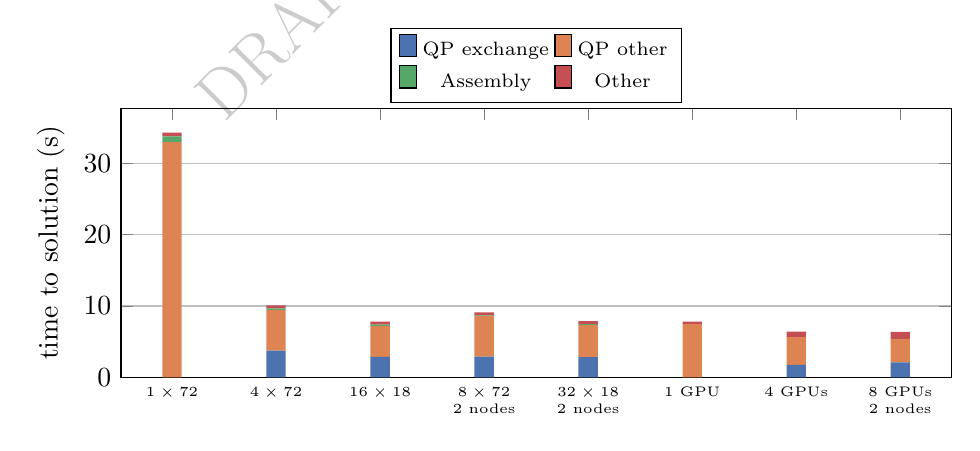
\begin{tikzpicture}
\begin{axis}[ybar stacked, bar width=7pt, width=\columnwidth, height=5.0cm,
  symbolic x coords={c0,c1,c2,c3,c4,c5,c6,c7}, xtick=data,
  xticklabels={{$1\times72$},{$4\times72$},{$16\times18$},{$8\times72$\\2 nodes},{$32\times18$\\2 nodes},{1 GPU},{4 GPUs},{8 GPUs\\2 nodes}}, xticklabel style={font=\tiny, align=center},
  ymin=0, ylabel={time to solution (\si{\second})}, ymajorgrids,
  legend style={font=\scriptsize, at={(0.5,1.02)}, anchor=south, legend columns=2},
  enlarge x limits=0.07]
\addplot[fill=LdpA, draw=none] coordinates {(c0,0.000) (c1,3.763) (c2,2.875) (c3,2.894) (c4,2.828) (c5,0.000) (c6,1.768) (c7,2.109)};
\addlegendentry{QP exchange}
\addplot[fill=LdpB, draw=none] coordinates {(c0,32.940) (c1,5.704) (c2,4.315) (c3,5.688) (c4,4.496) (c5,7.449) (c6,3.874) (c7,3.285)};
\addlegendentry{QP other}
\addplot[fill=LdpC, draw=none] coordinates {(c0,0.796) (c1,0.182) (c2,0.209) (c3,0.105) (c4,0.119) (c5,0.009) (c6,0.004) (c7,0.003)};
\addlegendentry{Assembly}
\addplot[fill=LdpD, draw=none] coordinates {(c0,0.529) (c1,0.435) (c2,0.400) (c3,0.428) (c4,0.428) (c5,0.338) (c6,0.759) (c7,0.989)};
\addlegendentry{Other}
\end{axis}
\end{tikzpicture}

\caption{Time to solution of FF200 refined (\dofsFFf{} dofs) by phase.}
\label{fig:breakdown}
\end{figure}

Table~\ref{tab:performance} and Figure~\ref{fig:per-iteration} give the cost per QP iteration and
the time to solution. The QP accounts for at least \qpShareFFf\% of the solve time on FF200 refined
in every configuration (Figure~\ref{fig:breakdown}), so the cost per QP iteration determines the
time to solution.

\paragraph{GPUs.} One GPU is the fastest configuration on \oneGpuBestCases{}; \bestElsewhere{}. Per case, the fastest Grace configuration takes
\gpuOverGraceMin{} to \gpuOverGraceMax{} times as long as the fastest GPU configuration.

\paragraph{Grace.} An empty OpenMP parallel region costs \regionCostWide\,\si{\micro\second} with
\machineCores{} threads per rank and \regionCostNarrow\,\si{\micro\second} with 18, as much as a pass
over a rank's unknowns. MPRGP's conjugate-gradient steps therefore share one region, and a QP
iteration of FF200 on $1\times72$ opens \regionsPerIteration{}. Their sums are not OpenMP reduction
clauses: GCC combines a clause of several variables under a global lock of its runtime, on which
the threads of a rank serialise. In a stand-in for the step on FF200's unknowns, with a
tridiagonal matrix in place of the tangent, a region per pass with such clauses costs
\standinRegionsOne{} and \standinRegionsFour\,\si{\micro\second} per step on $1\times72$ and
$4\times72$, one shared region \standinTeamOne{} and \standinTeamFour\,\si{\micro\second}. On one
node $4\times72$ costs \hostThreadsMin{} to \hostThreadsMax{} times as much per iteration as
$16\times18$, and more than $1\times72$ only on \fourSlowerThanOneCases{}, the case with the least
work per rank, where the stand-in's synchronisation accounts for \standinGap{} of the
\hostGapOneFour\,\si{\micro\second} difference.

\paragraph{Latency.} The cheapest iteration of each case costs \itBestMin{} to
\itBestMax\,\si{\micro\second}, while the work per iteration grows \dofsRatio-fold from the smallest
to the largest case: the QP iteration is latency bound. Its fixed cost is the two global reductions, the
ghost exchange, on Grace the three barriers and, on the GPU, the kernel launches and the transfer of each reduction's result to
the host. Adding ranks shrinks the work per rank but not these costs, which bounds the strong
scaling of every case.

\paragraph{Reference.} Utopia solved the four cases in \utopiaTimeFPc, \utopiaTimeFFc,
\utopiaTimeFPf{} and \utopiaTimeFFf\,\si{\second} on \utopiaRanks{} MPI ranks of an unrecorded
machine, with \utopiaNewtonFPc, \utopiaNewtonFFc, \utopiaNewtonFPf{} and \utopiaNewtonFFf{} Newton
steps. Without the machine and at different accuracies the times are no basis for a speed-up.

\paragraph{Load steps.} The overlap can instead be released over $n$ quasi-static pseudo-steps:
the bound admits a share of the starting penetration that falls linearly to zero, and each
pseudo-step is solved to convergence. Table~\ref{tab:release} compares $n=1$, 2 and 4 on
$4\times72$, with utopia's damped step and with full Newton steps under an Armijo line search; a
pseudo-step whose line search fails is retried with half its length. With the damped step a
pseudo-step takes \releasePerStepMin{} to \releasePerStepMax{} times as many Newton steps as the
single step, so two pseudo-steps take \releaseTwoMin{} to \releaseTwoMax{} and four
\releaseFourMin{} to \releaseFourMax{} times as long. In one step the Armijo rule solves
\armijoFasterCases{} \armijoGainMin{} to \armijoGainMax\% faster than the damped step, but on
\armijoCutbackCase{} its line search fails in every repeat and the retry makes the solve
\armijoCutbackSlower{} times as long. \armijoCutbackRuns{} of the \armijoRuns{} Armijo runs were
retried, none of the damped ones. The cases therefore remove the overlap in one damped step.

\paragraph{Single-precision tangent.} The tangent's values can be stored in single precision. Each
entry of an element matrix is computed in double and rounded once as it is added, so the matrix is
assembled in this format directly, without a copy in double; the operator application reads the
values into double and accumulates in double, and the vectors and the QP stay in double. This
halves the bytes of matrix values each operator application reads. Table~\ref{tab:precision}
compares the two precisions on one node in \precisionRuns{} runs that alternate between them per
repeat, with the build of Table~\ref{tab:performance}. Single precision lowers the cost per QP
iteration by \singleGpuOneMin{} to \singleGpuOneMax\% on one GPU, and on FF200 refined by
\singleRefinedGrace\% on $16\times18$ and \singleRefinedFour\% on four GPUs; there one GPU solves in
\solveSingleFFfGpuOne{} instead of \solveDoubleFFfGpuOne\,\si{\second}. With several ranks on the
smaller cases the change lies between \singleSmallMin{} and \singleSmallMax\%. The Newton step
counts are unchanged, and the median QP iteration count changes by at most \singleQpChange\%; in
\singleQpOutside{} of \singleQpConfigs{} configurations that is more than the spread between the
three double repeats, by at most \singleQpExcess{} percentage points. In the same configuration
the final displacement in single precision differs from the first double run by at most a
relative \agreeSingle{} on \convergedCases{}, while the double repeats differ from each other by
up to \agreeDouble{}; on \unconvergedCases{} the two figures are \agreeSingleUnconverged{} and
\agreeDoubleUnconverged{}. Double precision remains the default and is used everywhere else in
this paper.

\paragraph{Communication within a node.} As an option, the GPUs of one node exchange ghost values
by NCCL~\cite{nccl}, queued on the GPU's stream, and, where one node holds every rank, MPRGP's two
reductions complete on the GPU as well, so that an iteration returns to the host once, as on one
GPU. Between nodes GPU-aware MPI remains for both: there NCCL's messages took longer than MPI's
and, unless libfabric sends every message by rendezvous, delivered wrong values; with rendezvous,
its reductions over two nodes saved no time. Table~\ref{tab:nccl} compares the option with MPI in
\ncclRuns{} runs alternating per repeat; the Newton step counts are the same. On one node NCCL
lowers the cost per QP iteration by \ncclOneGainMin{} to \ncclOneGainMax\%, on two nodes, eight
GPUs, by \ncclEightGainMin{} to \ncclEightGainMax\%. Its set-up takes \ncclInitMin{} to
\ncclInitMax\,\si{\second} once per process, most of it in calls to the GPU driver, on a thread of
its own beside the rest of the set-up; the run waits for it, or is slowed by it, for
\ncclCostMin{} to \ncclCostMax\,\si{\second}, and the time to solution grows by \ncclExtraMin{}
to \ncclExtraMax\,\si{\second} on every case. The option repays its set-up after
\ncclBreakEvenMin{} to \ncclBreakEvenMax{} QP iterations a process. It is off by default.

\begin{table*}
\caption{Cost per QP iteration (\si{\micro\second}) and time to solution (\si{\second}), median of
\benchRepeats{} runs. Grace configurations are ranks $\times$ threads.}
\label{tab:performance}
\small
%% Generated by wip/ldp_containment/python/ldp_figures.py -- do not edit.
%% Regenerate with: make figures

\begin{tabular}{@{}llrrrrrrrr@{}}
\toprule
 & & \multicolumn{2}{c}{FF200} & \multicolumn{2}{c}{FP70 coarse} & \multicolumn{2}{c}{FP70} & \multicolumn{2}{c}{FF200 refined} \\
\cmidrule(lr){3-4}\cmidrule(lr){5-6}\cmidrule(lr){7-8}\cmidrule(lr){9-10}
Nodes & Configuration & \si{\micro\second} & \si{\second} & \si{\micro\second} & \si{\second} & \si{\micro\second} & \si{\second} & \si{\micro\second} & \si{\second} \\
\midrule
1 & $1\times72$ & \num{79} & \num{1.49} & \num{126} & \num{2.49} & \num{461} & \num{2.54} & \num{1169} & \num{34.3} \\
1 & $4\times72$ & \num{107} & \num{1.67} & \num{115} & \num{2.06} & \num{164} & \num{1.04} & \num{323} & \num{10.1} \\
1 & $16\times18$ & \num{103} & \num{1.69} & \num{124} & \num{2.31} & \num{170} & \num{1.19} & \num{249} & \num{7.80} \\
\addlinespace
2 & $8\times72$ & \num{138} & \num{2.11} & \num{125} & \num{2.29} & \num{168} & \num{1.11} & \num{303} & \num{9.12} \\
2 & $32\times18$ & \num{161} & \num{2.39} & \num{151} & \num{2.73} & \num{193} & \num{1.19} & \num{252} & \num{7.87} \\
\addlinespace
1 & 1 GPU & \num{86} & \num{1.32} & \num{98} & \num{1.75} & \num{174} & \num{1.06} & \num{281} & \num{7.80} \\
1 & 4 GPUs & \num{134} & \num{2.28} & \num{136} & \num{2.91} & \num{172} & \num{1.50} & \num{198} & \num{6.40} \\
\addlinespace
2 & 8 GPUs & \num{159} & \num{2.91} & \num{170} & \num{3.41} & \num{175} & \num{1.67} & \num{181} & \num{6.39} \\
\bottomrule
\end{tabular}

\end{table*}

\begin{table*}
\caption{The tangent in double and in single precision on one node: cost per QP iteration and
time to solution, median of \benchRepeats{} runs each.}
\label{tab:precision}
\small
\setlength{\tabcolsep}{3.5pt}
%% Generated by wip/ldp_containment/python/ldp_figures.py -- do not edit.
%% Regenerate with: make figures

\begin{tabular}{@{}llrrrrr@{}}
\toprule
 & & \multicolumn{3}{c}{\si{\micro\second} per QP iteration} & \multicolumn{2}{c}{Solve (\si{\second})} \\
\cmidrule(lr){3-5}\cmidrule(l){6-7}
Case & Configuration & double & single & change & double & single \\
\midrule
FF200 & $16\times18$ & \num{104} & \num{101} & \num{-2.3}\% & \num{1.64} & \num{1.64} \\
 & 1 GPU & \num{85} & \num{67} & \num{-21.1}\% & \num{1.36} & \num{1.09} \\
 & 4 GPUs & \num{133} & \num{133} & \num{-0.1}\% & \num{2.34} & \num{2.26} \\
\addlinespace
FP70 coarse & $16\times18$ & \num{127} & \num{124} & \num{-2.4}\% & \num{2.33} & \num{2.28} \\
 & 1 GPU & \num{98} & \num{81} & \num{-17.1}\% & \num{1.77} & \num{1.53} \\
 & 4 GPUs & \num{135} & \num{134} & \num{-0.3}\% & \num{2.98} & \num{2.93} \\
\addlinespace
FP70 & $16\times18$ & \num{172} & \num{170} & \num{-1.3}\% & \num{1.15} & \num{1.19} \\
 & 1 GPU & \num{175} & \num{146} & \num{-16.7}\% & \num{1.07} & \num{0.916} \\
 & 4 GPUs & \num{176} & \num{167} & \num{-5.1}\% & \num{1.52} & \num{1.56} \\
\addlinespace
FF200 refined & $16\times18$ & \num{243} & \num{224} & \num{-7.8}\% & \num{7.94} & \num{6.84} \\
 & 1 GPU & \num{277} & \num{224} & \num{-19.3}\% & \num{8.31} & \num{6.64} \\
 & 4 GPUs & \num{198} & \num{179} & \num{-9.6}\% & \num{6.49} & \num{5.78} \\
\bottomrule
\end{tabular}

\end{table*}

\begin{table*}
\caption{Communication within a node by MPI and by NCCL: cost per QP iteration, what NCCL's set-up
costs a run (the longer set-up and the wait at the first communication) and the QP iterations
that repay it, and time to solution (set-up and solve), median of \benchRepeats{} runs each.}
\label{tab:nccl}
\small
%% Generated by wip/ldp_containment/python/ldp_figures.py -- do not edit.
%% Regenerate with: make figures

\begin{tabular}{@{}llrrrrrrr@{}}
\toprule
 & & \multicolumn{3}{c}{\si{\micro\second} per QP iteration} & \multicolumn{2}{c}{NCCL's set-up} & \multicolumn{2}{c}{To solution (\si{\second})} \\
\cmidrule(lr){3-5}\cmidrule(lr){6-7}\cmidrule(l){8-9}
Case & Configuration & MPI & NCCL & change & \si{\second} & repaid after & MPI & NCCL \\
\midrule
FF200 & 4 GPUs & \num{133} & \num{97} & \num{-27.4}\% & \num{3.1} & \num{86000} & \num{6.64} & \num{9.68} \\
 & 8 GPUs, 2 nodes & \num{160} & \num{135} & \num{-15.6}\% & \num{3.2} & \num{129000} & \num{3.36} & \num{6.82} \\
\addlinespace
FP70 coarse & 4 GPUs & \num{135} & \num{98} & \num{-27.2}\% & \num{3.5} & \num{95000} & \num{6.98} & \num{10.3} \\
 & 8 GPUs, 2 nodes & \num{173} & \num{138} & \num{-20.4}\% & \num{3.5} & \num{98000} & \num{3.76} & \num{7.34} \\
\addlinespace
FP70 & 4 GPUs & \num{175} & \num{147} & \num{-15.9}\% & \num{3.2} & \num{116000} & \num{5.97} & \num{9.45} \\
 & 8 GPUs, 2 nodes & \num{175} & \num{147} & \num{-16.2}\% & \num{3.9} & \num{136000} & \num{2.03} & \num{6.08} \\
\addlinespace
FF200 refined & 4 GPUs & \num{195} & \num{183} & \num{-6.3}\% & \num{2.9} & \num{231000} & \num{11.3} & \num{13.9} \\
 & 8 GPUs, 2 nodes & \num{182} & \num{169} & \num{-6.6}\% & \num{3.4} & \num{281000} & \num{7.04} & \num{10.3} \\
\bottomrule
\end{tabular}

\end{table*}

\begin{table*}
\caption{The overlap released over 1, 2 and 4 pseudo-steps, each solved to convergence, on
$4\times72$: Newton steps (those of failed attempts included) and solve time, median of
\releaseRepeats{} runs each, alternating per repeat.}
\label{tab:release}
\small
%% Generated by wip/ldp_containment/python/ldp_figures.py -- do not edit.
%% Regenerate with: make figures

\begin{tabular}{@{}llrrrrrr@{}}
\toprule
 & & \multicolumn{2}{c}{1 step} & \multicolumn{2}{c}{2 steps} & \multicolumn{2}{c}{4 steps} \\
\cmidrule(lr){3-4}\cmidrule(lr){5-6}\cmidrule(lr){7-8}
Case & Line search & Newton & \si{\second} & Newton & \si{\second} & Newton & \si{\second} \\
\midrule
FF200 & damped & \num{20} & \num{1.74} & \num{38} & \num{3.50} & \num{85} & \num{7.46} \\
 & Armijo & \num{17} & \num{1.40} & \num{35} & \num{2.84} & \num{63} & \num{6.02} \\
\addlinespace
FP70 coarse & damped & \num{13} & \num{2.38} & \num{28} & \num{4.61} & \num{60} & \num{9.04} \\
 & Armijo & \num{25} & \num{6.51} & \num{22} & \num{3.22} & \num{45} & \num{6.31} \\
\addlinespace
FP70 & damped & \num{13} & \num{3.93} & \num{26} & \num{8.44} & \num{55} & \num{15.9} \\
 & Armijo & \num{9} & \num{3.01} & \num{31} & \num{6.24} & \num{55} & \num{12.0} \\
\addlinespace
FF200 refined & damped & \num{16} & \num{9.84} & \num{33} & \num{18.4} & \num{59} & \num{37.9} \\
 & Armijo & \num{12} & \num{6.63} & \num{23} & \num{12.5} & \num{48} & \num{26.2} \\
\bottomrule
\end{tabular}

\end{table*}

\begin{figure*}
\centering
%% Generated by wip/ldp_containment/python/ldp_figures.py -- do not edit.
%% Regenerate with: make figures

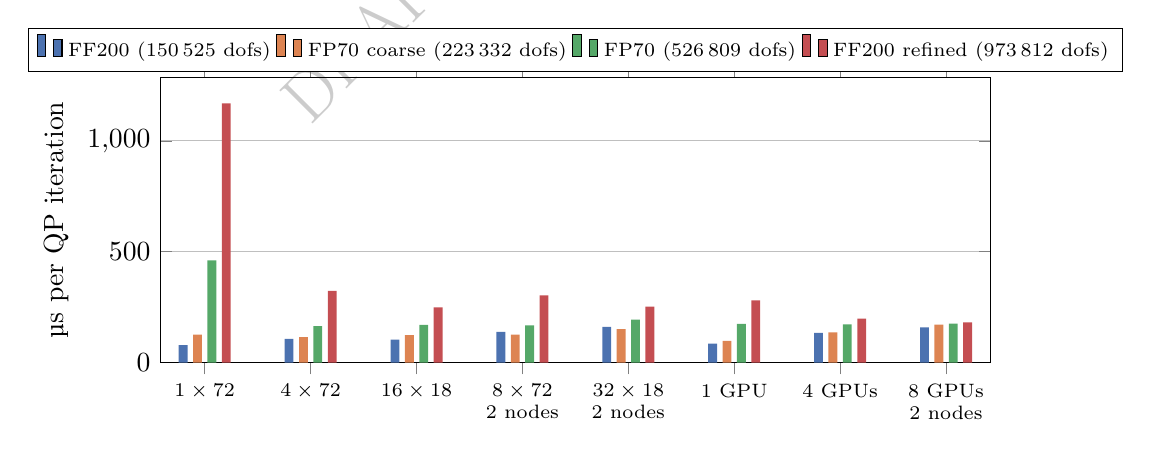
\begin{tikzpicture}
\begin{axis}[ybar, bar width=3.2pt, width=\textwidth, height=5.2cm,
  symbolic x coords={c0,c1,c2,c3,c4,c5,c6,c7}, xtick=data,
  xticklabels={{$1\times72$},{$4\times72$},{$16\times18$},{$8\times72$\\2 nodes},{$32\times18$\\2 nodes},{1 GPU},{4 GPUs},{8 GPUs\\2 nodes}}, xticklabel style={font=\scriptsize, align=center},
  ymin=0, ylabel={\si{\micro\second} per QP iteration}, ymajorgrids,
  legend style={font=\scriptsize, at={(0.5,1.02)}, anchor=south, legend columns=4},
  enlarge x limits=0.06]
\addplot[fill=LdpA, draw=none] coordinates {(c0,78.7) (c1,106.6) (c2,103.5) (c3,137.8) (c4,161.1) (c5,85.5) (c6,133.9) (c7,159.0)};
\addlegendentry{FF200 (\num{150525} dofs)}
\addplot[fill=LdpB, draw=none] coordinates {(c0,125.7) (c1,114.6) (c2,123.7) (c3,125.3) (c4,151.0) (c5,98.1) (c6,135.6) (c7,170.5)};
\addlegendentry{FP70 coarse (\num{223332} dofs)}
\addplot[fill=LdpC, draw=none] coordinates {(c0,460.9) (c1,163.7) (c2,170.2) (c3,167.9) (c4,193.2) (c5,174.3) (c6,171.7) (c7,175.1)};
\addlegendentry{FP70 (\num{526809} dofs)}
\addplot[fill=LdpD, draw=none] coordinates {(c0,1169.0) (c1,323.1) (c2,249.3) (c3,303.2) (c4,252.4) (c5,280.8) (c6,197.6) (c7,180.7)};
\addlegendentry{FF200 refined (\num{973812} dofs)}
\end{axis}
\end{tikzpicture}

\caption{Cost per QP iteration of every configuration.}
\label{fig:per-iteration}
\end{figure*}

\section{Through four pump strokes}
\label{sec:strokes}

The contained valves are the start of a transient simulation: the pressure in the pump chamber
lifts each valve off its seat and pushes it back. We follow the two valves of FF200
(\dofsFFc{} dofs, \trContactNodes{} contact nodes) through \trStrokes{} strokes of
\trStrokeMs\,\si{\milli\second} on one GPU, and those of FF200 refined (\dofsFFf{} dofs, the same
valves meshed finer) on a full node, \trGpusRefined{} GPUs.

\paragraph{Material.} The valves are EPDM, modelled as Mooney--Rivlin,
$\psi = C_{10}(\bar I_1-3) + C_{01}(\bar I_2-3) + \tfrac{K}{2}(J-1)^2$, whose isochoric part
relaxes by a Prony series, $\mu(t) = \mu_\infty\bigl(g_\infty + \sum_k g_k e^{-t/\tau_k}\bigr)/g_\infty$,
with one stress-like history variable per term and quadrature point. The series is the broadband one
of \citet{felhos2008}, 15 terms with $\tau_k$ from \SI{1.8e-27}{\second} to \SI{1610}{\second} and
$g_\infty = \num{2.24e-3}$, with $C_{01}/C_{10}=4$. The moduli are scaled so that the relaxed
small-strain stiffness is that of the containment runs ($E=\SI{9.174}{\mega\pascal}$, $\nu=0.4$):
$2g_\infty(C_{10}+C_{01}) = \SI{3.276}{\mega\pascal}$, and $K=\SI{15.29}{\mega\pascal}$ does not
relax. The density is \SI{1150}{\kilo\gram\per\cubic\metre}, with a lumped mass matrix.

\paragraph{Two simulations.} The first is the containment of Section~\ref{sec:problem}
with this material, quasi-static over four pseudo-steps of \SI{2.5e4}{\second}, far longer than
every relaxation time, so the valves end relaxed, as when assembled long before the pump runs.
Its obstacle is a distance field with a larger margin, which includes the pressure valve's cage
and the suction valve's stop, so that the free valves are held at the top of their travel. The
outlet pressure of \SI{90543}{\pascal} is ramped onto the pressure valve with the release and
holds it on its seat. The second simulation starts at rest from that state, with the Prony
history relaxed there. Each valve carries the pressure difference across it as a vertical
traction on the disc of its chamber-side face inside the seat ring: the chamber pressure $p(t)$
on both, less the outlet pressure on the pressure valve. $p(t)$ is the measured membrane pressure
of the FP70 pump (no FF200 data exist), \trEnd\,\si{\milli\second} long
(Figure~\ref{fig:strokes}, top). The nominal step is \trDtMs\,\si{\milli\second},
\trStepsNominal{} steps; Newton's iteration stops when the forces are below \SI{1e-6}{\newton}
and the penetration below \SI{1}{\nano\metre}. A step that fails is retried with half its length,
up to eight times; the displacement of every step is written.

\paragraph{Time integration.} SFEM's contact-stabilised Newmark scheme,
damped by $\gamma=0.6$, carries the acceleration of the material forces alone from step to step.
At a node on its seat that acceleration is balanced by the contact force it does not see, so the
predicted velocity points into the seat, and the predicted start of the next step inverts elements
there: its \trStepsNewmark{} steps took \trFailedNewmark{} failed attempts
(Table~\ref{tab:strokes}). BDF2 avoids this: its velocity is derived from the displacements,
$v_{n+1} = c_0u_{n+1} + c_1u_n + c_2u_{n-1}$, and its acceleration from the velocities with the
same coefficients, so a reaction leaves no trace in the next step's data. With variable steps,
$\omega = \Delta t_{n+1}/\Delta t_n$,
\begin{equation}
  c_0 = \frac{1+2\omega}{(1+\omega)\Delta t_{n+1}},\quad
  c_1 = -\frac{1+\omega}{\Delta t_{n+1}},\quad
  c_2 = \frac{\omega^2}{(1+\omega)\Delta t_{n+1}},
\end{equation}
the tangent is $K + c_0^2M$, and the scheme is zero-stable for $\omega < 1+\sqrt2$~\cite{grigorieff1983}:
after a cut-back the step grows back by at most a factor of two per step. BDF2 is L-stable, so it damps
the high frequencies the impacts excite. Newton's iteration starts at $u_n + \Delta t\,v_n$,
the displacement the last velocity carries on to, rather than at $u_n$: a valve in flight
otherwise starts each step as if it had stopped.

\paragraph{The valves.} Table~\ref{tab:valves} and Figure~\ref{fig:strokes} give the motion; a
valve is counted open while its centre is more than \trLiftOpen\,\si{\micro\metre} from where it
rests at $t=0$. When the chamber pressure rises above the outlet's, the pressure valve lifts by
\trPvPeakMin{} to \trPvPeakMax\,\si{\milli\metre} onto its cage and stays there for the
discharge; when it falls below the suction side's, the suction valve opens by \trSvPeakMin{} to
\trSvPeakMax\,\si{\milli\metre} onto its stop. On closing, the suction valve bounces off its seat
and is open again for up to \trSvReboundMax\,\si{\milli\second}. The response is periodic: each
opening and closing falls within \trPvPeriodic\,\si{\milli\second} (pressure valve) and
\trSvPeriodic\,\si{\milli\second} (suction valve) of the first stroke's, a period later.
Figure~\ref{fig:stills} shows the valves at rest, on the cage, both seated between discharge and
suction, and the suction valve on its stop. The three runs of Table~\ref{tab:strokes} open and close
the valves within \trEventSpread\,\si{\milli\second} of each other and agree on the largest lift per
stroke to \trPeakSpread\%. A run is not reproducible to the bit, since the GPU assembles with
atomic additions, and the impacts amplify the rounding differences.

\paragraph{Cost.} Table~\ref{tab:strokes} gives the cost of the \trStrokes{} strokes on one GPU
with \machineCores{} cores, and Table~\ref{tab:changes} the effect of each change since the first
BDF2 run, measured over the first \trWindowFinish{} or \trWindowStart\,\si{\milli\second} against
the build before it. In the QP, finishing each reduction in the last thread block instead of a
second kernel saves \trFinishGain\% per Newton step, storing the tangent in float32 a further
\trFloatGain\%, and running consecutive conjugate-gradient steps of MPRGP on the device, in a CUDA
graph whose loop the GPU decides without returning to the host, \trRunsGain\%. Newton's start at
$u_n+\Delta t\,v_n$ cuts the failed attempts over \trWindowStart\,\si{\milli\second} from
\trFailedBaseWindow{} to \trFailedStartWindow{} and the QP time from \trQpBaseWindow{} to
\trQpStartWindow\,\si{\second}; a non-monotone line search on its own fails \trFailedNonmonoWindow{}
times and gains nothing in combination. Writing only the displacement instead of every field
lowers the output from \trWritePerStepBdf{} to \trWritePerStepFinal\,\si{\milli\second} per step.
Together the \trStrokes{} strokes take \trSteppingFinal\,\si{\second}, \trSpeedBdf{} times less
than the first BDF2 run and \trSpeedNewmark{} times less than Newmark, with \trFailedFinal{} failed
attempts in \trStepsFinal{} steps; the QP takes \trQpShareFinal\% of it, and
\trOtherFinal\,\si{\second} are spent outside the traced Newton solve and output.

\paragraph{Two resolutions.} FF200 refined has \trResDofsRatio{} times the unknowns of FF200 and runs
on the \trGpusRefined{} GPUs of a node, a rank each, with simulation 1 on its Grace CPUs
($4\times72$). Two parts of the set-up needed the distributed mesh: each rank reads the starting
displacement by the ids its nodes have in the file, and a traction's share at a node that another
rank owns is added there, since the sidesets keep each face on one rank while the volume operators
complete an owned row from the aura's elements. The refined valves move as FF200's
(Table~\ref{tab:valves}, Figures~\ref{fig:strokes} and~\ref{fig:resolutions}): after simulation 1
they rest within \trResRest\,\si{\micro\metre} of FF200's positions, they open and close within
\trResEventShift\,\si{\milli\second} of FF200's instants, and their largest lift per stroke differs
from FF200's by at most \trResPeakDiff\%. The coarser mesh resolves the valves' motion.
Table~\ref{tab:resolutions} compares the cost. The four strokes take \trSteppingRefined\,\si{\second},
\trResSteppingRatio{} times as long as FF200's on one GPU. A QP needs \trResItsRatio{} times as many
iterations per Newton step, against the \trResExpectedIts{} by which the element size shrinks, the
growth a conjugate-gradient iteration count shows on a second-order operator. An iteration costs
\trResPerItRatio{} times as much: each GPU holds \trResWorkPerGpu{} times FF200's unknowns, the
ranks add a ghost exchange and two global reductions to every iteration
(Section~\ref{sec:parallel}), and MPRGP's device runs, which need a single rank, are not used. The
refined run fails \trFailedRefined{} attempts against \trFailedFinal{}, all of them line searches at
the pressure valve's impacts, \trResFailFirst{} to \trResFailLast\,\si{\milli\second} into a stroke
(Figure~\ref{fig:strokes}, bottom). Writing the displacement, gathered on rank 0, takes
\trResWriteRatio{} times as long per step.

\begin{figure*}
\centering
%% Generated by wip/ldp_containment/python/ldp_figures.py -- do not edit.
%% Regenerate with: make figures

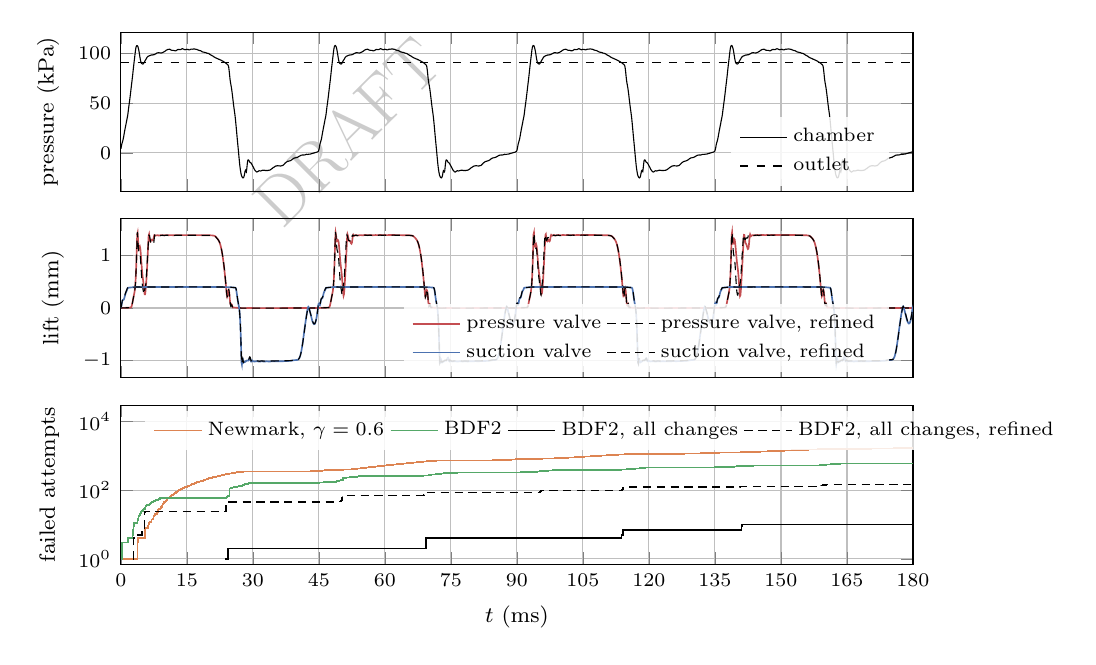
\begin{tikzpicture}
\begin{groupplot}[group style={group size=1 by 3, vertical sep=0.35cm, xticklabels at=edge bottom},
  width=0.96\textwidth, height=3.6cm, xmin=0, xmax=180, xtick distance=15, xmajorgrids, ymajorgrids,
  tick label style={font=\scriptsize}, label style={font=\footnotesize},
  legend style={font=\scriptsize, draw=none, fill=white, fill opacity=0.85, text opacity=1}, legend cell align=left]
\nextgroupplot[ylabel={pressure (\si{\kilo\pascal})}, legend pos=south east]
\addplot[black, thin] coordinates {(0.0000,4.147) (0.1000,6.387) (0.2000,8.847) (0.3000,10.384) (0.4000,11.922) (0.5000,13.547) (0.6000,15.699) (0.7000,18.203) (0.8000,20.795) (0.9000,23.255) (1.0000,25.495) (1.1000,27.647) (1.2000,29.887) (1.3000,32.259) (1.4000,34.456) (1.5000,36.564) (1.6000,39.463) (1.7000,43.241) (1.8000,46.623) (1.9000,49.873) (2.0000,53.256) (2.1000,56.814) (2.2000,60.416) (2.3000,64.237) (2.4000,68.103) (2.5000,71.617) (2.6000,75.394) (2.7000,79.347) (2.8000,83.608) (2.9000,87.606) (3.0000,91.427) (3.1000,94.985) (3.2000,98.806) (3.3000,102.496) (3.4000,105.527) (3.5000,107.108) (3.6000,107.767) (3.7000,107.811) (3.8000,107.460) (3.9000,106.274) (4.0000,104.561) (4.1000,102.452) (4.2000,99.817) (4.3000,96.918) (4.4000,94.238) (4.5000,92.174) (4.6000,90.592) (4.7000,89.890) (4.8000,89.714) (4.9000,89.362) (5.0000,89.319) (5.1000,89.538) (5.2000,90.241) (5.3000,90.988) (5.4000,91.822) (5.5000,92.701) (5.6000,93.404) (5.7000,94.150) (5.8000,94.809) (5.9000,95.776) (6.0000,96.303) (6.1000,96.654) (6.2000,97.093) (6.3000,97.181) (6.4000,97.533) (6.5000,97.621) (6.6000,97.796) (6.7000,97.972) (6.8000,98.236) (6.9000,98.367) (7.0000,98.372) (7.1000,98.307) (7.2000,98.411) (7.3000,98.626) (7.4000,98.641) (7.5000,98.614) (7.6000,98.856) (7.7000,99.135) (7.8000,99.313) (7.9000,99.582) (8.0000,99.752) (8.1000,100.014) (8.2000,100.374) (8.3000,100.432) (8.4000,100.577) (8.5000,100.691) (8.6000,100.686) (8.7000,100.607) (8.8000,100.520) (8.9000,100.476) (9.0000,100.388) (9.1000,100.379) (9.2000,100.352) (9.3000,100.531) (9.4000,100.681) (9.5000,100.915) (9.6000,101.066) (9.7000,101.331) (9.8000,101.563) (9.9000,101.857) (10.0000,102.076) (10.1000,102.409) (10.2000,102.794) (10.3000,103.180) (10.4000,103.265) (10.5000,103.649) (10.6000,103.902) (10.7000,103.911) (10.8000,103.999) (10.9000,104.041) (11.0000,104.156) (11.1000,104.110) (11.2000,103.929) (11.3000,103.539) (11.4000,103.291) (11.5000,103.155) (11.6000,103.101) (11.7000,103.054) (11.8000,103.063) (11.9000,103.077) (12.0000,102.945) (12.1000,102.807) (12.2000,102.702) (12.3000,102.584) (12.4000,102.543) (12.5000,102.660) (12.6000,102.852) (12.7000,103.255) (12.8000,103.437) (12.9000,103.841) (13.0000,103.867) (13.1000,103.872) (13.2000,103.919) (13.3000,103.844) (13.4000,103.731) (13.5000,103.735) (13.6000,103.823) (13.7000,104.103) (13.8000,104.406) (13.9000,104.618) (14.0000,104.645) (14.1000,104.561) (14.2000,104.261) (14.3000,104.163) (14.4000,103.832) (14.5000,103.758) (14.6000,103.606) (14.7000,103.770) (14.8000,103.952) (14.9000,104.003) (15.0000,104.114) (15.1000,103.990) (15.2000,103.858) (15.3000,103.929) (15.4000,103.550) (15.5000,103.507) (15.6000,103.529) (15.7000,103.732) (15.8000,104.030) (15.9000,104.179) (16.0000,104.231) (16.1000,104.244) (16.2000,104.173) (16.3000,104.307) (16.4000,104.219) (16.5000,104.464) (16.6000,104.514) (16.7000,104.394) (16.8000,104.320) (16.9000,104.193) (17.0000,104.176) (17.1000,104.038) (17.2000,103.946) (17.3000,103.875) (17.4000,103.513) (17.5000,103.457) (17.6000,103.216) (17.7000,103.013) (17.8000,102.940) (17.9000,102.896) (18.0000,102.748) (18.1000,102.647) (18.2000,102.434) (18.3000,102.157) (18.4000,101.771) (18.5000,101.594) (18.6000,101.403) (18.7000,101.310) (18.8000,101.195) (18.9000,101.165) (19.0000,100.894) (19.1000,100.919) (19.2000,100.827) (19.3000,100.761) (19.4000,100.426) (19.5000,100.298) (19.6000,100.094) (19.7000,100.085) (19.8000,99.949) (19.9000,99.886) (20.0000,99.764) (20.1000,99.430) (20.2000,99.079) (20.3000,98.751) (20.4000,98.507) (20.5000,98.208) (20.6000,97.993) (20.7000,97.733) (20.8000,97.513) (20.9000,97.335) (21.0000,97.001) (21.1000,96.635) (21.2000,96.325) (21.3000,96.090) (21.4000,95.939) (21.5000,95.521) (21.6000,95.413) (21.7000,95.236) (21.8000,94.974) (21.9000,94.787) (22.0000,94.742) (22.1000,94.404) (22.2000,94.125) (22.3000,94.073) (22.4000,93.941) (22.5000,93.579) (22.6000,93.469) (22.7000,93.190) (22.8000,93.050) (22.9000,92.838) (23.0000,92.506) (23.1000,92.275) (23.2000,92.142) (23.3000,91.725) (23.4000,91.459) (23.5000,91.240) (23.6000,90.939) (23.7000,90.707) (23.8000,90.375) (23.9000,89.980) (24.0000,89.598) (24.1000,89.277) (24.2000,88.882) (24.3000,88.484) (24.4000,87.779) (24.5000,86.063) (24.6000,82.623) (24.7000,78.364) (24.8000,74.043) (24.9000,70.903) (25.0000,68.498) (25.1000,66.021) (25.2000,63.031) (25.3000,59.594) (25.4000,55.859) (25.5000,52.094) (25.6000,48.385) (25.7000,45.024) (25.8000,41.910) (25.9000,38.727) (26.0000,34.973) (26.1000,30.618) (26.2000,25.847) (26.3000,20.982) (26.4000,16.178) (26.5000,11.502) (26.6000,6.890) (26.7000,2.280) (26.8000,-2.495) (26.9000,-7.162) (27.0000,-11.802) (27.1000,-15.389) (27.2000,-18.302) (27.3000,-20.886) (27.4000,-22.676) (27.5000,-23.626) (27.6000,-24.560) (27.7000,-25.014) (27.8000,-24.921) (27.9000,-24.470) (28.0000,-23.359) (28.1000,-21.151) (28.2000,-18.625) (28.3000,-17.491) (28.4000,-18.418) (28.5000,-19.137) (28.6000,-16.182) (28.7000,-11.761) (28.8000,-8.070) (28.9000,-6.971) (29.0000,-7.021) (29.1000,-7.646) (29.2000,-8.388) (29.3000,-9.314) (29.4000,-9.612) (29.5000,-9.808) (29.6000,-10.280) (29.7000,-11.010) (29.8000,-11.786) (29.9000,-12.810) (30.0000,-13.498) (30.1000,-14.214) (30.2000,-15.265) (30.3000,-16.215) (30.4000,-16.904) (30.5000,-17.558) (30.6000,-18.083) (30.7000,-18.589) (30.8000,-18.975) (30.9000,-19.146) (31.0000,-19.007) (31.1000,-18.683) (31.2000,-18.431) (31.3000,-18.139) (31.4000,-17.860) (31.5000,-17.943) (31.6000,-18.058) (31.7000,-18.116) (31.8000,-17.991) (31.9000,-17.887) (32.0000,-17.672) (32.1000,-17.582) (32.2000,-17.408) (32.3000,-17.411) (32.4000,-17.416) (32.5000,-17.461) (32.6000,-17.390) (32.7000,-17.476) (32.8000,-17.650) (32.9000,-17.640) (33.0000,-17.721) (33.1000,-17.586) (33.2000,-17.584) (33.3000,-17.670) (33.4000,-17.622) (33.5000,-17.464) (33.6000,-17.351) (33.7000,-17.365) (33.8000,-17.218) (33.9000,-17.148) (34.0000,-16.807) (34.1000,-16.480) (34.2000,-16.125) (34.3000,-15.839) (34.4000,-15.604) (34.5000,-15.092) (34.6000,-14.812) (34.7000,-14.537) (34.8000,-14.269) (34.9000,-13.969) (35.0000,-13.577) (35.1000,-13.304) (35.2000,-13.149) (35.3000,-13.113) (35.4000,-13.032) (35.5000,-12.861) (35.6000,-12.819) (35.7000,-12.848) (35.8000,-12.916) (35.9000,-12.940) (36.0000,-12.914) (36.1000,-12.990) (36.2000,-13.200) (36.3000,-13.107) (36.4000,-12.963) (36.5000,-12.928) (36.6000,-12.769) (36.7000,-12.665) (36.8000,-12.482) (36.9000,-12.141) (37.0000,-11.751) (37.1000,-11.234) (37.2000,-10.819) (37.3000,-10.312) (37.4000,-9.869) (37.5000,-9.569) (37.6000,-9.256) (37.7000,-8.888) (37.8000,-8.659) (37.9000,-8.381) (38.0000,-8.360) (38.1000,-8.317) (38.2000,-8.113) (38.3000,-7.952) (38.4000,-7.927) (38.5000,-7.702) (38.6000,-7.462) (38.7000,-7.286) (38.8000,-6.912) (38.9000,-6.638) (39.0000,-6.267) (39.1000,-5.954) (39.2000,-5.620) (39.3000,-5.345) (39.4000,-5.095) (39.5000,-5.098) (39.6000,-4.946) (39.7000,-4.837) (39.8000,-4.800) (39.9000,-4.682) (40.0000,-4.462) (40.1000,-4.331) (40.2000,-4.257) (40.3000,-4.001) (40.4000,-3.661) (40.5000,-3.364) (40.6000,-3.191) (40.7000,-2.951) (40.8000,-2.664) (40.9000,-2.434) (41.0000,-2.271) (41.1000,-2.212) (41.2000,-2.094) (41.3000,-2.167) (41.4000,-2.005) (41.5000,-2.165) (41.6000,-2.090) (41.7000,-1.924) (41.8000,-1.984) (41.9000,-1.860) (42.0000,-1.626) (42.1000,-1.462) (42.2000,-1.327) (42.3000,-1.463) (42.4000,-1.506) (42.5000,-1.442) (42.6000,-1.309) (42.7000,-1.330) (42.8000,-1.156) (42.9000,-1.129) (43.0000,-1.124) (43.1000,-1.041) (43.2000,-0.961) (43.3000,-0.764) (43.4000,-0.672) (43.5000,-0.465) (43.6000,-0.357) (43.7000,-0.287) (43.8000,-0.091) (43.9000,-0.063) (44.0000,0.123) (44.1000,0.356) (44.2000,0.355) (44.3000,0.580) (44.4000,0.628) (44.5000,0.787) (44.6000,0.910) (44.7000,1.111) (44.8000,1.306) (44.9000,1.940) (45.0000,3.367) (45.1000,5.385) (45.2000,8.026) (45.3000,9.869) (45.4000,11.244) (45.5000,12.955) (45.6000,14.692) (45.7000,17.260) (45.8000,19.780) (45.9000,22.233) (46.0000,24.579) (46.1000,26.806) (46.2000,28.970) (46.3000,31.350) (46.4000,33.696) (46.5000,35.718) (46.6000,38.095) (46.7000,41.568) (46.8000,45.409) (46.9000,48.613) (47.0000,51.843) (47.1000,55.290) (47.2000,58.933) (47.3000,62.729) (47.4000,66.520) (47.5000,70.169) (47.6000,73.882) (47.7000,77.762) (47.8000,82.006) (47.9000,85.988) (48.0000,89.881) (48.1000,93.539) (48.2000,97.297) (48.3000,101.144) (48.4000,104.345) (48.5000,106.637) (48.6000,107.602) (48.7000,107.935) (48.8000,107.564) (48.9000,106.771) (49.0000,105.349) (49.1000,103.423) (49.2000,100.834) (49.3000,97.996) (49.4000,95.285) (49.5000,92.978) (49.6000,91.100) (49.7000,90.125) (49.8000,89.786) (49.9000,89.427) (50.0000,89.278) (50.1000,89.383) (50.2000,89.877) (50.3000,90.667) (50.4000,91.584) (50.5000,92.430) (50.6000,93.083) (50.7000,93.793) (50.8000,94.482) (50.9000,95.395) (51.0000,96.052) (51.1000,96.551) (51.2000,96.994) (51.3000,97.260) (51.4000,97.357) (51.5000,97.538) (51.6000,97.836) (51.7000,97.972) (51.8000,98.091) (51.9000,98.296) (52.0000,98.367) (52.1000,98.365) (52.2000,98.497) (52.3000,98.489) (52.4000,98.598) (52.5000,98.644) (52.6000,98.850) (52.7000,99.006) (52.8000,99.235) (52.9000,99.474) (53.0000,99.703) (53.1000,99.942) (53.2000,100.242) (53.3000,100.287) (53.4000,100.592) (53.5000,100.695) (53.6000,100.667) (53.7000,100.607) (53.8000,100.577) (53.9000,100.504) (54.0000,100.445) (54.1000,100.388) (54.2000,100.311) (54.3000,100.437) (54.4000,100.592) (54.5000,100.875) (54.6000,100.951) (54.7000,101.202) (54.8000,101.445) (54.9000,101.764) (55.0000,101.977) (55.1000,102.219) (55.2000,102.657) (55.3000,103.029) (55.4000,103.243) (55.5000,103.572) (55.6000,103.770) (55.7000,103.902) (55.8000,103.990) (55.9000,104.062) (56.0000,104.145) (56.1000,104.093) (56.2000,103.971) (56.3000,103.703) (56.4000,103.419) (56.5000,103.269) (56.6000,103.144) (56.7000,103.067) (56.8000,102.982) (56.9000,103.035) (57.0000,103.049) (57.1000,102.978) (57.2000,102.687) (57.3000,102.584) (57.4000,102.569) (57.5000,102.599) (57.6000,102.848) (57.7000,103.056) (57.8000,103.333) (57.9000,103.621) (58.0000,103.886) (58.1000,103.915) (58.2000,103.981) (58.3000,103.801) (58.4000,103.726) (58.5000,103.755) (58.6000,103.814) (58.7000,103.998) (58.8000,104.282) (58.9000,104.528) (59.0000,104.649) (59.1000,104.583) (59.2000,104.485) (59.3000,104.165) (59.4000,104.031) (59.5000,103.770) (59.6000,103.613) (59.7000,103.751) (59.8000,103.800) (59.9000,104.104) (60.0000,104.121) (60.1000,104.010) (60.2000,103.943) (60.3000,103.889) (60.4000,103.636) (60.5000,103.535) (60.6000,103.507) (60.7000,103.726) (60.8000,103.876) (60.9000,104.165) (61.0000,104.288) (61.1000,104.168) (61.2000,104.165) (61.3000,104.273) (61.4000,104.295) (61.5000,104.406) (61.6000,104.431) (61.7000,104.434) (61.8000,104.437) (61.9000,104.235) (62.0000,104.133) (62.1000,104.147) (62.2000,104.031) (62.3000,103.937) (62.4000,103.627) (62.5000,103.406) (62.6000,103.326) (62.7000,103.071) (62.8000,102.958) (62.9000,102.948) (63.0000,102.880) (63.1000,102.701) (63.2000,102.477) (63.3000,102.270) (63.4000,101.920) (63.5000,101.672) (63.6000,101.440) (63.7000,101.396) (63.8000,101.289) (63.9000,101.122) (64.0000,100.935) (64.1000,101.029) (64.2000,100.912) (64.3000,100.818) (64.4000,100.556) (64.5000,100.243) (64.6000,100.184) (64.7000,100.166) (64.8000,100.094) (64.9000,99.819) (65.0000,99.744) (65.1000,99.574) (65.2000,99.219) (65.3000,98.858) (65.4000,98.663) (65.5000,98.312) (65.6000,98.068) (65.7000,97.829) (65.8000,97.613) (65.9000,97.411) (66.0000,97.162) (66.1000,96.724) (66.2000,96.483) (66.3000,96.212) (66.4000,95.951) (66.5000,95.686) (66.6000,95.424) (66.7000,95.273) (66.8000,95.089) (66.9000,94.895) (67.0000,94.737) (67.1000,94.457) (67.2000,94.266) (67.3000,94.235) (67.4000,93.975) (67.5000,93.597) (67.6000,93.559) (67.7000,93.309) (67.8000,93.052) (67.9000,92.968) (68.0000,92.597) (68.1000,92.388) (68.2000,92.174) (68.3000,91.777) (68.4000,91.610) (68.5000,91.362) (68.6000,91.141) (68.7000,90.749) (68.8000,90.528) (68.9000,90.126) (69.0000,89.726) (69.1000,89.430) (69.2000,89.028) (69.3000,88.634) (69.4000,88.123) (69.5000,87.005) (69.6000,84.069) (69.7000,80.190) (69.8000,75.665) (69.9000,72.018) (70.0000,69.389) (70.1000,67.116) (70.2000,64.268) (70.3000,60.960) (70.4000,57.445) (70.5000,53.596) (70.6000,49.857) (70.7000,46.374) (70.8000,43.154) (70.9000,39.996) (71.0000,36.528) (71.1000,32.404) (71.2000,27.785) (71.3000,22.926) (71.4000,18.149) (71.5000,13.329) (71.6000,8.723) (71.7000,4.111) (71.8000,-0.544) (71.9000,-5.369) (72.0000,-10.005) (72.1000,-13.980) (72.2000,-17.238) (72.3000,-19.868) (72.4000,-22.175) (72.5000,-23.264) (72.6000,-24.282) (72.7000,-24.750) (72.8000,-25.052) (72.9000,-24.787) (73.0000,-23.962) (73.1000,-22.128) (73.2000,-19.506) (73.3000,-17.688) (73.4000,-18.053) (73.5000,-18.923) (73.6000,-17.880) (73.7000,-13.356) (73.8000,-9.432) (73.9000,-7.119) (74.0000,-7.010) (74.1000,-7.327) (74.2000,-8.033) (74.3000,-9.031) (74.4000,-9.558) (74.5000,-9.687) (74.6000,-10.047) (74.7000,-10.703) (74.8000,-11.530) (74.9000,-12.377) (75.0000,-13.241) (75.1000,-13.939) (75.2000,-14.871) (75.3000,-15.775) (75.4000,-16.727) (75.5000,-17.302) (75.6000,-17.848) (75.7000,-18.353) (75.8000,-18.913) (75.9000,-19.084) (76.0000,-19.147) (76.1000,-18.762) (76.2000,-18.597) (76.3000,-18.217) (76.4000,-17.923) (76.5000,-17.891) (76.6000,-17.940) (76.7000,-18.123) (76.8000,-18.012) (76.9000,-17.969) (77.0000,-17.761) (77.1000,-17.624) (77.2000,-17.470) (77.3000,-17.392) (77.4000,-17.363) (77.5000,-17.407) (77.6000,-17.399) (77.7000,-17.493) (77.8000,-17.617) (77.9000,-17.669) (78.0000,-17.671) (78.1000,-17.620) (78.2000,-17.552) (78.3000,-17.805) (78.4000,-17.640) (78.5000,-17.464) (78.6000,-17.418) (78.7000,-17.468) (78.8000,-17.303) (78.9000,-17.128) (79.0000,-16.960) (79.1000,-16.570) (79.2000,-16.311) (79.3000,-15.963) (79.4000,-15.800) (79.5000,-15.235) (79.6000,-14.876) (79.7000,-14.677) (79.8000,-14.383) (79.9000,-14.071) (80.0000,-13.757) (80.1000,-13.447) (80.2000,-13.183) (80.3000,-13.116) (80.4000,-13.050) (80.5000,-12.995) (80.6000,-12.920) (80.7000,-12.738) (80.8000,-12.831) (80.9000,-12.969) (81.0000,-12.925) (81.1000,-13.041) (81.2000,-13.133) (81.3000,-13.142) (81.4000,-13.041) (81.5000,-12.912) (81.6000,-12.783) (81.7000,-12.768) (81.8000,-12.587) (81.9000,-12.341) (82.0000,-11.876) (82.1000,-11.395) (82.2000,-11.014) (82.3000,-10.473) (82.4000,-10.070) (82.5000,-9.680) (82.6000,-9.374) (82.7000,-8.991) (82.8000,-8.794) (82.9000,-8.496) (83.0000,-8.434) (83.1000,-8.328) (83.2000,-8.150) (83.3000,-8.102) (83.4000,-7.904) (83.5000,-7.789) (83.6000,-7.611) (83.7000,-7.344) (83.8000,-6.989) (83.9000,-6.802) (84.0000,-6.479) (84.1000,-6.080) (84.2000,-5.698) (84.3000,-5.405) (84.4000,-5.305) (84.5000,-5.064) (84.6000,-4.917) (84.7000,-4.923) (84.8000,-4.785) (84.9000,-4.682) (85.0000,-4.605) (85.1000,-4.416) (85.2000,-4.322) (85.3000,-4.048) (85.4000,-3.767) (85.5000,-3.524) (85.6000,-3.334) (85.7000,-2.993) (85.8000,-2.788) (85.9000,-2.464) (86.0000,-2.342) (86.1000,-2.285) (86.2000,-2.139) (86.3000,-2.156) (86.4000,-2.022) (86.5000,-2.102) (86.6000,-2.062) (86.7000,-2.029) (86.8000,-2.003) (86.9000,-1.842) (87.0000,-1.703) (87.1000,-1.500) (87.2000,-1.344) (87.3000,-1.538) (87.4000,-1.462) (87.5000,-1.399) (87.6000,-1.414) (87.7000,-1.378) (87.8000,-1.218) (87.9000,-1.124) (88.0000,-1.152) (88.1000,-1.093) (88.2000,-1.060) (88.3000,-0.795) (88.4000,-0.713) (88.5000,-0.535) (88.6000,-0.443) (88.7000,-0.289) (88.8000,-0.200) (88.9000,-0.041) (89.0000,0.053) (89.1000,0.272) (89.2000,0.257) (89.3000,0.549) (89.4000,0.548) (89.5000,0.640) (89.6000,0.871) (89.7000,1.016) (89.8000,1.292) (89.9000,1.637) (90.0000,2.607) (90.1000,4.538) (90.2000,6.955) (90.3000,9.222) (90.4000,10.656) (90.5000,12.277) (90.6000,13.889) (90.7000,16.227) (90.8000,18.723) (90.9000,21.271) (91.0000,23.703) (91.1000,25.939) (91.2000,28.081) (91.3000,30.377) (91.4000,32.759) (91.5000,34.871) (91.6000,37.025) (91.7000,40.130) (91.8000,44.010) (91.9000,47.285) (92.0000,50.514) (92.1000,53.920) (92.2000,57.522) (92.3000,61.184) (92.4000,64.989) (92.5000,68.801) (92.6000,72.366) (92.7000,76.178) (92.8000,80.234) (92.9000,84.400) (93.0000,88.368) (93.1000,92.140) (93.2000,95.750) (93.3000,99.604) (93.4000,103.125) (93.5000,105.964) (93.6000,107.309) (93.7000,107.857) (93.8000,107.726) (93.9000,107.285) (94.0000,105.995) (94.1000,104.200) (94.2000,101.917) (94.3000,99.214) (94.4000,96.371) (94.5000,93.797) (94.6000,91.784) (94.7000,90.415) (94.8000,89.847) (94.9000,89.615) (95.0000,89.319) (95.1000,89.334) (95.2000,89.630) (95.3000,90.385) (95.4000,91.201) (95.5000,92.023) (95.6000,92.823) (95.7000,93.527) (95.8000,94.260) (95.9000,94.996) (96.0000,95.872) (96.1000,96.401) (96.2000,96.771) (96.3000,97.177) (96.4000,97.212) (96.5000,97.533) (96.6000,97.716) (96.7000,97.858) (96.8000,97.992) (96.9000,98.255) (97.0000,98.367) (97.1000,98.396) (97.2000,98.450) (97.3000,98.411) (97.4000,98.602) (97.5000,98.663) (97.6000,98.758) (97.7000,98.891) (97.8000,99.169) (97.9000,99.366) (98.0000,99.642) (98.1000,99.833) (98.2000,100.063) (98.3000,100.302) (98.4000,100.546) (98.5000,100.649) (98.6000,100.667) (98.7000,100.638) (98.8000,100.607) (98.9000,100.520) (99.0000,100.476) (99.1000,100.388) (99.2000,100.331) (99.3000,100.367) (99.4000,100.546) (99.5000,100.760) (99.6000,100.915) (99.7000,101.097) (99.8000,101.363) (99.9000,101.637) (100.0000,101.889) (100.1000,102.106) (100.2000,102.500) (100.3000,102.862) (100.4000,103.224) (100.5000,103.388) (100.6000,103.663) (100.7000,103.902) (100.8000,103.959) (100.9000,104.047) (101.0000,104.082) (101.1000,104.108) (101.2000,104.046) (101.3000,103.879) (101.4000,103.525) (101.5000,103.315) (101.6000,103.155) (101.7000,103.079) (101.8000,102.982) (101.9000,103.039) (102.0000,103.100) (102.1000,102.992) (102.2000,102.717) (102.3000,102.630) (102.4000,102.584) (102.5000,102.562) (102.6000,102.777) (102.7000,102.885) (102.8000,103.269) (102.9000,103.466) (103.0000,103.884) (103.1000,103.915) (103.2000,103.943) (103.3000,103.825) (103.4000,103.773) (103.5000,103.755) (103.6000,103.783) (103.7000,103.880) (103.8000,104.154) (103.9000,104.438) (104.0000,104.639) (104.1000,104.626) (104.2000,104.561) (104.3000,104.195) (104.4000,104.148) (104.5000,103.788) (104.6000,103.694) (104.7000,103.670) (104.8000,103.770) (104.9000,104.090) (105.0000,104.075) (105.1000,104.073) (105.2000,103.990) (105.3000,103.858) (105.4000,103.832) (105.5000,103.550) (105.6000,103.507) (105.7000,103.649) (105.8000,103.766) (105.9000,104.120) (106.0000,104.251) (106.1000,104.162) (106.2000,104.196) (106.3000,104.214) (106.4000,104.330) (106.5000,104.276) (106.6000,104.416) (106.7000,104.497) (106.8000,104.442) (106.9000,104.282) (107.0000,104.147) (107.1000,104.198) (107.2000,104.062) (107.3000,103.946) (107.4000,103.776) (107.5000,103.422) (107.6000,103.421) (107.7000,103.160) (107.8000,102.996) (107.9000,102.964) (108.0000,102.920) (108.1000,102.731) (108.2000,102.561) (108.3000,102.380) (108.4000,102.089) (108.5000,101.737) (108.6000,101.537) (108.7000,101.427) (108.8000,101.310) (108.9000,101.127) (109.0000,101.086) (109.1000,101.013) (109.2000,100.943) (109.3000,100.827) (109.4000,100.684) (109.5000,100.288) (109.6000,100.282) (109.7000,100.166) (109.8000,100.109) (109.9000,99.834) (110.0000,99.791) (110.1000,99.709) (110.2000,99.360) (110.3000,99.009) (110.4000,98.737) (110.5000,98.434) (110.6000,98.153) (110.7000,97.939) (110.8000,97.700) (110.9000,97.478) (111.0000,97.283) (111.1000,96.884) (111.2000,96.605) (111.3000,96.293) (111.4000,95.999) (111.5000,95.866) (111.6000,95.455) (111.7000,95.348) (111.8000,95.203) (111.9000,94.959) (112.0000,94.742) (112.1000,94.614) (112.2000,94.391) (112.3000,94.220) (112.4000,94.007) (112.5000,93.758) (112.6000,93.579) (112.7000,93.415) (112.8000,93.100) (112.9000,93.033) (113.0000,92.742) (113.1000,92.473) (113.2000,92.207) (113.3000,91.966) (113.4000,91.711) (113.5000,91.446) (113.6000,91.227) (113.7000,90.835) (113.8000,90.654) (113.9000,90.284) (114.0000,89.888) (114.1000,89.548) (114.2000,89.186) (114.3000,88.790) (114.4000,88.382) (114.5000,87.584) (114.6000,85.428) (114.7000,81.863) (114.8000,77.439) (114.9000,73.306) (115.0000,70.367) (115.1000,68.071) (115.2000,65.442) (115.3000,62.342) (115.4000,58.922) (115.5000,55.105) (115.6000,51.359) (115.7000,47.723) (115.8000,44.391) (115.9000,41.253) (116.0000,38.007) (116.1000,34.130) (116.2000,29.689) (116.3000,24.883) (116.4000,20.060) (116.5000,15.204) (116.6000,10.568) (116.7000,5.956) (116.8000,1.353) (116.9000,-3.493) (117.0000,-8.092) (117.1000,-12.535) (117.2000,-16.052) (117.3000,-18.831) (117.4000,-21.415) (117.5000,-22.890) (117.6000,-23.841) (117.7000,-24.587) (117.8000,-25.079) (117.9000,-24.908) (118.0000,-24.341) (118.1000,-22.975) (118.2000,-20.571) (118.3000,-18.250) (118.4000,-17.658) (118.5000,-18.551) (118.6000,-18.869) (118.7000,-15.184) (118.8000,-11.011) (118.9000,-7.621) (119.0000,-6.995) (119.1000,-7.089) (119.2000,-7.764) (119.3000,-8.631) (119.4000,-9.432) (119.5000,-9.626) (119.6000,-9.875) (119.7000,-10.423) (119.8000,-11.217) (119.9000,-11.958) (120.0000,-12.972) (120.1000,-13.663) (120.2000,-14.429) (120.3000,-15.415) (120.4000,-16.450) (120.5000,-17.026) (120.6000,-17.640) (120.7000,-18.168) (120.8000,-18.755) (120.9000,-19.011) (121.0000,-19.168) (121.1000,-18.911) (121.2000,-18.670) (121.3000,-18.332) (121.4000,-18.064) (121.5000,-17.860) (121.6000,-17.919) (121.7000,-18.102) (121.8000,-18.075) (121.9000,-17.991) (122.0000,-17.853) (122.1000,-17.655) (122.2000,-17.546) (122.3000,-17.386) (122.4000,-17.363) (122.5000,-17.392) (122.6000,-17.442) (122.7000,-17.462) (122.8000,-17.540) (122.9000,-17.673) (123.0000,-17.640) (123.1000,-17.679) (123.2000,-17.563) (123.3000,-17.751) (123.4000,-17.649) (123.5000,-17.526) (123.6000,-17.464) (123.7000,-17.446) (123.8000,-17.350) (123.9000,-17.149) (124.0000,-17.093) (124.1000,-16.712) (124.2000,-16.450) (124.3000,-16.095) (124.4000,-15.839) (124.5000,-15.447) (124.6000,-14.993) (124.7000,-14.780) (124.8000,-14.484) (124.9000,-14.195) (125.0000,-13.921) (125.1000,-13.546) (125.2000,-13.245) (125.3000,-13.127) (125.4000,-13.094) (125.5000,-13.056) (125.6000,-12.909) (125.7000,-12.727) (125.8000,-12.824) (125.9000,-12.961) (126.0000,-12.940) (126.1000,-13.010) (126.2000,-13.026) (126.3000,-13.181) (126.4000,-13.091) (126.5000,-12.919) (126.6000,-12.864) (126.7000,-12.793) (126.8000,-12.651) (126.9000,-12.452) (127.0000,-12.025) (127.1000,-11.618) (127.2000,-11.166) (127.3000,-10.688) (127.4000,-10.246) (127.5000,-9.797) (127.6000,-9.495) (127.7000,-9.164) (127.8000,-8.874) (127.9000,-8.629) (128.0000,-8.429) (128.1000,-8.338) (128.2000,-8.258) (128.3000,-8.137) (128.4000,-7.908) (128.5000,-7.891) (128.6000,-7.688) (128.7000,-7.403) (128.8000,-7.165) (128.9000,-6.898) (129.0000,-6.609) (129.1000,-6.195) (129.2000,-5.831) (129.3000,-5.545) (129.4000,-5.369) (129.5000,-5.052) (129.6000,-4.979) (129.7000,-4.946) (129.8000,-4.792) (129.9000,-4.728) (130.0000,-4.682) (130.1000,-4.462) (130.2000,-4.331) (130.3000,-4.148) (130.4000,-3.928) (130.5000,-3.647) (130.6000,-3.364) (130.7000,-3.085) (130.8000,-2.896) (130.9000,-2.558) (131.0000,-2.419) (131.1000,-2.295) (131.2000,-2.197) (131.3000,-2.113) (131.4000,-2.102) (131.5000,-2.022) (131.6000,-2.093) (131.7000,-2.090) (131.8000,-1.972) (131.9000,-1.889) (132.0000,-1.801) (132.1000,-1.565) (132.2000,-1.426) (132.3000,-1.471) (132.4000,-1.441) (132.5000,-1.434) (132.6000,-1.464) (132.7000,-1.357) (132.8000,-1.294) (132.9000,-1.134) (133.0000,-1.152) (133.1000,-1.124) (133.2000,-1.065) (133.3000,-0.877) (133.4000,-0.746) (133.5000,-0.637) (133.6000,-0.465) (133.7000,-0.312) (133.8000,-0.270) (133.9000,-0.047) (134.0000,-0.026) (134.1000,0.154) (134.2000,0.284) (134.3000,0.434) (134.4000,0.532) (134.5000,0.605) (134.6000,0.825) (134.7000,0.946) (134.8000,1.227) (134.9000,1.395) (135.0000,2.101) (135.1000,3.753) (135.2000,5.872) (135.3000,8.454) (135.4000,10.127) (135.5000,11.578) (135.6000,13.243) (135.7000,15.184) (135.8000,17.726) (135.9000,20.294) (136.0000,22.754) (136.1000,25.039) (136.2000,27.224) (136.3000,29.422) (136.4000,31.800) (136.5000,34.074) (136.6000,36.131) (136.7000,38.768) (136.8000,42.413) (136.9000,46.012) (137.0000,49.242) (137.1000,52.553) (137.2000,56.057) (137.3000,59.667) (137.4000,63.484) (137.5000,67.328) (137.6000,70.886) (137.7000,74.632) (137.8000,78.539) (137.9000,82.813) (138.0000,86.805) (138.1000,90.665) (138.2000,94.253) (138.3000,98.047) (138.4000,101.836) (138.5000,104.978) (138.6000,106.890) (138.7000,107.690) (138.8000,107.881) (138.9000,107.521) (139.0000,106.531) (139.1000,104.956) (139.2000,102.953) (139.3000,100.339) (139.4000,97.454) (139.5000,94.742) (139.6000,92.569) (139.7000,90.822) (139.8000,89.984) (139.9000,89.755) (140.0000,89.393) (140.1000,89.297) (140.2000,89.453) (140.3000,90.062) (140.4000,90.819) (140.5000,91.695) (140.6000,92.570) (140.7000,93.248) (140.8000,93.983) (140.9000,94.638) (141.0000,95.609) (141.1000,96.182) (141.2000,96.597) (141.3000,97.043) (141.4000,97.212) (141.5000,97.471) (141.6000,97.572) (141.7000,97.812) (141.8000,97.972) (141.9000,98.175) (142.0000,98.342) (142.1000,98.367) (142.2000,98.293) (142.3000,98.425) (142.4000,98.608) (142.5000,98.621) (142.6000,98.596) (142.7000,98.850) (142.8000,99.085) (142.9000,99.270) (143.0000,99.527) (143.1000,99.718) (143.2000,99.974) (143.3000,100.366) (143.4000,100.353) (143.5000,100.568) (143.6000,100.695) (143.7000,100.691) (143.8000,100.607) (143.9000,100.529) (144.0000,100.480) (144.1000,100.397) (144.2000,100.388) (144.3000,100.334) (144.4000,100.500) (144.5000,100.629) (144.6000,100.910) (144.7000,101.019) (144.8000,101.281) (144.9000,101.500) (145.0000,101.815) (145.1000,102.033) (145.2000,102.318) (145.3000,102.725) (145.4000,103.122) (145.5000,103.243) (145.6000,103.622) (145.7000,103.881) (145.8000,103.902) (145.9000,103.990) (146.0000,104.038) (146.1000,104.163) (146.2000,104.117) (146.3000,103.957) (146.4000,103.582) (146.5000,103.307) (146.6000,103.173) (146.7000,103.121) (146.8000,103.067) (146.9000,103.054) (147.0000,103.057) (147.1000,102.954) (147.2000,102.888) (147.3000,102.711) (147.4000,102.584) (147.5000,102.545) (147.6000,102.615) (147.7000,102.848) (147.8000,103.206) (147.9000,103.394) (148.0000,103.769) (148.1000,103.862) (148.2000,103.867) (148.3000,103.959) (148.4000,103.849) (148.5000,103.726) (148.6000,103.731) (148.7000,103.814) (148.8000,104.051) (148.9000,104.357) (149.0000,104.586) (149.1000,104.649) (149.2000,104.564) (149.3000,104.347) (149.4000,104.165) (149.5000,103.900) (149.6000,103.770) (149.7000,103.597) (149.8000,103.768) (149.9000,103.866) (150.0000,104.008) (150.1000,104.121) (150.2000,103.992) (150.3000,103.872) (150.4000,103.937) (150.5000,103.562) (150.6000,103.511) (150.7000,103.507) (150.8000,103.726) (150.9000,103.953) (151.0000,104.165) (151.1000,104.266) (151.2000,104.240) (151.3000,104.165) (151.4000,104.289) (151.5000,104.223) (151.6000,104.463) (151.7000,104.503) (151.8000,104.392) (151.9000,104.368) (152.0000,104.220) (152.1000,104.155) (152.2000,104.052) (152.3000,103.959) (152.4000,103.916) (152.5000,103.578) (152.6000,103.453) (152.7000,103.270) (152.8000,103.037) (152.9000,102.939) (153.0000,102.901) (153.1000,102.787) (153.2000,102.684) (153.3000,102.463) (153.4000,102.218) (153.5000,101.826) (153.6000,101.638) (153.7000,101.404) (153.8000,101.324) (153.9000,101.245) (154.0000,101.169) (154.1000,100.880) (154.2000,100.933) (154.3000,100.841) (154.4000,100.797) (154.5000,100.507) (154.6000,100.291) (154.7000,100.096) (154.8000,100.094) (154.9000,100.027) (155.0000,99.891) (155.1000,99.768) (155.2000,99.501) (155.3000,99.149) (155.4000,98.784) (155.5000,98.582) (155.6000,98.261) (155.7000,98.035) (155.8000,97.775) (155.9000,97.556) (156.0000,97.377) (156.1000,97.090) (156.2000,96.676) (156.3000,96.382) (156.4000,96.157) (156.5000,95.951) (156.6000,95.594) (156.7000,95.424) (156.8000,95.258) (156.9000,95.008) (157.0000,94.834) (157.1000,94.761) (157.2000,94.426) (157.3000,94.132) (157.4000,94.144) (157.5000,93.975) (157.6000,93.581) (157.7000,93.514) (157.8000,93.257) (157.9000,93.052) (158.0000,92.909) (158.1000,92.547) (158.2000,92.333) (158.3000,92.174) (158.4000,91.747) (158.5000,91.501) (158.6000,91.276) (158.7000,91.036) (158.8000,90.735) (158.9000,90.455) (159.0000,90.058) (159.1000,89.657) (159.2000,89.357) (159.3000,88.960) (159.4000,88.567) (159.5000,87.958) (159.6000,86.572) (159.7000,83.358) (159.8000,79.276) (159.9000,74.826) (160.0000,71.453) (160.1000,68.941) (160.2000,66.577) (160.3000,63.671) (160.4000,60.275) (160.5000,56.637) (160.6000,52.840) (160.7000,49.095) (160.8000,45.684) (160.9000,42.543) (161.0000,39.389) (161.1000,35.770) (161.2000,31.522) (161.3000,26.814) (161.4000,21.938) (161.5000,17.157) (161.6000,12.423) (161.7000,7.813) (161.8000,3.200) (161.9000,-1.515) (162.0000,-6.252) (162.1000,-10.965) (162.2000,-14.701) (162.3000,-17.770) (162.4000,-20.376) (162.5000,-22.438) (162.6000,-23.434) (162.7000,-24.483) (162.8000,-24.919) (162.9000,-24.959) (163.0000,-24.615) (163.1000,-23.680) (163.2000,-21.664) (163.3000,-19.037) (163.4000,-17.495) (163.5000,-18.254) (163.6000,-19.140) (163.7000,-17.057) (163.8000,-12.545) (163.9000,-8.638) (164.0000,-6.986) (164.1000,-7.010) (164.2000,-7.503) (164.3000,-8.194) (164.4000,-9.184) (164.5000,-9.589) (164.6000,-9.746) (164.7000,-10.157) (164.8000,-10.842) (164.9000,-11.644) (165.0000,-12.617) (165.1000,-13.358) (165.2000,-14.055) (165.3000,-15.084) (165.4000,-15.995) (165.5000,-16.804) (165.6000,-17.448) (165.7000,-17.979) (165.8000,-18.460) (165.9000,-18.942) (166.0000,-19.120) (166.1000,-19.080) (166.2000,-18.711) (166.3000,-18.516) (166.4000,-18.187) (166.5000,-17.869) (166.6000,-17.938) (166.7000,-18.008) (166.8000,-18.123) (166.9000,-17.994) (167.0000,-17.924) (167.1000,-17.703) (167.2000,-17.607) (167.3000,-17.434) (167.4000,-17.416) (167.5000,-17.411) (167.6000,-17.455) (167.7000,-17.380) (167.8000,-17.469) (167.9000,-17.632) (168.0000,-17.645) (168.1000,-17.719) (168.2000,-17.604) (168.3000,-17.552) (168.4000,-17.711) (168.5000,-17.640) (168.6000,-17.464) (168.7000,-17.346) (168.8000,-17.399) (168.9000,-17.265) (169.0000,-17.152) (169.1000,-16.888) (169.2000,-16.520) (169.3000,-16.187) (169.4000,-15.858) (169.5000,-15.712) (169.6000,-15.172) (169.7000,-14.845) (169.8000,-14.599) (169.9000,-14.330) (170.0000,-14.020) (170.1000,-13.637) (170.2000,-13.369) (170.3000,-13.168) (170.4000,-13.116) (170.5000,-13.031) (170.6000,-12.875) (170.7000,-12.876) (170.8000,-12.834) (170.9000,-12.876) (171.0000,-12.945) (171.1000,-12.901) (171.2000,-12.993) (171.3000,-13.193) (171.4000,-13.124) (171.5000,-13.002) (171.6000,-12.935) (171.7000,-12.767) (171.8000,-12.699) (171.9000,-12.526) (172.0000,-12.243) (172.1000,-11.830) (172.2000,-11.310) (172.3000,-10.925) (172.4000,-10.388) (172.5000,-9.957) (172.6000,-9.630) (172.7000,-9.324) (172.8000,-8.920) (172.9000,-8.710) (173.0000,-8.391) (173.1000,-8.388) (173.2000,-8.328) (173.3000,-8.114) (173.4000,-8.010) (173.5000,-7.928) (173.6000,-7.732) (173.7000,-7.529) (173.8000,-7.330) (173.9000,-6.939) (174.0000,-6.695) (174.1000,-6.357) (174.2000,-6.031) (174.3000,-5.668) (174.4000,-5.350) (174.5000,-5.166) (174.6000,-5.112) (174.7000,-4.941) (174.8000,-4.878) (174.9000,-4.809) (175.0000,-4.682) (175.1000,-4.485) (175.2000,-4.344) (175.3000,-4.301) (175.4000,-4.034) (175.5000,-3.693) (175.6000,-3.389) (175.7000,-3.267) (175.8000,-2.980) (175.9000,-2.736) (176.0000,-2.450) (176.1000,-2.278) (176.2000,-2.239) (176.3000,-2.098) (176.4000,-2.175) (176.5000,-2.005) (176.6000,-2.167) (176.7000,-2.086) (176.8000,-1.933) (176.9000,-2.003) (177.0000,-1.866) (177.1000,-1.670) (177.2000,-1.485) (177.3000,-1.306) (177.4000,-1.492) (177.5000,-1.510) (177.6000,-1.421) (177.7000,-1.318) (177.8000,-1.356) (177.9000,-1.182) (178.0000,-1.124) (178.1000,-1.129) (178.2000,-1.045) (178.3000,-1.016) (178.4000,-0.781) (178.5000,-0.695) (178.6000,-0.475) (178.7000,-0.398) (178.8000,-0.289) (178.9000,-0.139) (179.0000,-0.065) (179.1000,0.088) (179.2000,0.355) (179.3000,0.301) (179.4000,0.584) (179.5000,0.619) (179.6000,0.732) (179.7000,0.886) (179.8000,1.050) (179.9000,1.292) (180.0000,1.785)};
\addlegendentry{chamber}
\addplot[black, dashed, thin, domain=0:180, samples=2] {90.5430};
\addlegendentry{outlet}
\nextgroupplot[ylabel={lift (\si{\milli\metre})}, legend pos=south east, legend columns=2]
\addplot[LdpD, semithick] coordinates {(0.0000,0.00000) (0.1000,0.00072) (0.2000,0.00101) (0.3000,0.00120) (0.4000,0.00141) (0.5000,0.00161) (0.6000,0.00188) (0.7000,0.00221) (0.8000,0.00254) (0.9000,0.00286) (1.0000,0.00317) (1.1000,0.00347) (1.2000,0.00379) (1.3000,0.00413) (1.4000,0.00446) (1.5000,0.00479) (1.6000,0.00523) (1.7000,0.00580) (1.8000,0.00634) (1.9000,0.00688) (2.0000,0.00747) (2.1000,0.00818) (2.2000,0.00912) (2.3000,0.01143) (2.4000,0.02497) (2.5000,0.05399) (2.6000,0.09398) (2.7000,0.13760) (2.8000,0.18081) (2.9000,0.22252) (3.0000,0.26353) (3.1000,0.30838) (3.2000,0.37079) (3.3000,0.47078) (3.4000,0.62575) (3.5000,0.84258) (3.6000,1.11887) (3.7000,1.40345) (3.8000,1.43766) (3.9000,1.29721) (4.0000,1.17939) (4.1000,1.14789) (4.2000,1.16721) (4.3000,1.17774) (4.4000,1.14111) (4.5000,1.05551) (4.6000,0.94034) (4.7000,0.81945) (4.8000,0.71258) (4.9000,0.62734) (5.0000,0.55761) (5.1000,0.48987) (5.2000,0.41443) (5.3000,0.33008) (5.4000,0.26341) (5.5000,0.26360) (5.6000,0.32756) (5.7000,0.42479) (5.8000,0.54284) (5.9000,0.68464) (6.0000,0.84997) (6.1000,1.02997) (6.2000,1.21229) (6.3000,1.38256) (6.4000,1.40891) (6.5000,1.34155) (6.6000,1.28488) (6.7000,1.27049) (6.8000,1.28474) (6.9000,1.30189) (7.0000,1.30536) (7.1000,1.29748) (7.2000,1.29045) (7.3000,1.29502) (7.4000,1.31991) (7.5000,1.36795) (7.6000,1.38955) (7.7000,1.38244) (7.8000,1.37865) (7.9000,1.38375) (8.0000,1.38750) (8.1000,1.38776) (8.2000,1.38886) (8.3000,1.39173) (8.4000,1.39058) (8.5000,1.38573) (8.6000,1.38341) (8.7000,1.38457) (8.8000,1.38648) (8.9000,1.38790) (9.0000,1.38905) (9.1000,1.39015) (9.2000,1.39104) (9.3000,1.39153) (9.4000,1.39108) (9.5000,1.38969) (9.6000,1.38764) (9.7000,1.38604) (9.8000,1.38616) (9.9000,1.38777) (10.0000,1.38962) (10.1000,1.39103) (10.2000,1.39197) (10.3000,1.39253) (10.4000,1.39252) (10.5000,1.39223) (10.6000,1.39157) (10.7000,1.39050) (10.8000,1.38984) (10.9000,1.39000) (11.0000,1.39075) (11.1000,1.39150) (11.2000,1.39193) (11.3000,1.39204) (11.4000,1.39208) (11.5000,1.39208) (11.6000,1.39175) (11.7000,1.39098) (11.8000,1.39014) (11.9000,1.38964) (12.0000,1.38956) (12.1000,1.38987) (12.2000,1.39037) (12.3000,1.39077) (12.4000,1.39105) (12.5000,1.39133) (12.6000,1.39155) (12.7000,1.39174) (12.8000,1.39157) (12.9000,1.39134) (13.0000,1.39104) (13.1000,1.39093) (13.2000,1.39121) (13.3000,1.39157) (13.4000,1.39178) (13.5000,1.39194) (13.6000,1.39211) (13.7000,1.39231) (13.8000,1.39241) (13.9000,1.39227) (14.0000,1.39191) (14.1000,1.39152) (14.2000,1.39123) (14.3000,1.39127) (14.4000,1.39134) (14.5000,1.39148) (14.6000,1.39160) (14.7000,1.39184) (14.8000,1.39209) (14.9000,1.39209) (15.0000,1.39203) (15.1000,1.39185) (15.2000,1.39160) (15.3000,1.39158) (15.4000,1.39139) (15.5000,1.39138) (15.6000,1.39162) (15.7000,1.39200) (15.8000,1.39233) (15.9000,1.39243) (16.0000,1.39230) (16.1000,1.39211) (16.2000,1.39192) (16.3000,1.39190) (16.4000,1.39180) (16.5000,1.39187) (16.6000,1.39195) (16.7000,1.39190) (16.8000,1.39192) (16.9000,1.39201) (17.0000,1.39213) (17.1000,1.39209) (17.2000,1.39196) (17.3000,1.39186) (17.4000,1.39161) (17.5000,1.39155) (17.6000,1.39149) (17.7000,1.39136) (17.8000,1.39131) (17.9000,1.39135) (18.0000,1.39128) (18.1000,1.39119) (18.2000,1.39106) (18.3000,1.39085) (18.4000,1.39056) (18.5000,1.39039) (18.6000,1.39029) (18.7000,1.39018) (18.8000,1.39003) (18.9000,1.38994) (19.0000,1.38972) (19.1000,1.38968) (19.2000,1.38970) (19.3000,1.38965) (19.4000,1.38939) (19.5000,1.38924) (19.6000,1.38920) (19.7000,1.38929) (19.8000,1.38926) (19.9000,1.38917) (20.0000,1.38905) (20.1000,1.38873) (20.2000,1.38832) (20.3000,1.38800) (20.4000,1.38779) (20.5000,1.38745) (20.6000,1.38700) (20.7000,1.38626) (20.8000,1.38529) (20.9000,1.38433) (21.0000,1.38314) (21.1000,1.38152) (21.2000,1.37925) (21.3000,1.37558) (21.4000,1.37040) (21.5000,1.36325) (21.6000,1.35472) (21.7000,1.34561) (21.8000,1.33601) (21.9000,1.32588) (22.0000,1.31568) (22.1000,1.30455) (22.2000,1.29108) (22.3000,1.27494) (22.4000,1.25603) (22.5000,1.23321) (22.6000,1.20595) (22.7000,1.17385) (22.8000,1.13706) (22.9000,1.09570) (23.0000,1.04931) (23.1000,0.99765) (23.2000,0.94119) (23.3000,0.87948) (23.4000,0.81218) (23.5000,0.73943) (23.6000,0.66135) (23.6500,0.62029) (23.7500,0.53451) (23.8500,0.44387) (23.9500,0.34810) (24.0500,0.26030) (24.1500,0.21909) (24.2500,0.24431) (24.3000,0.27601) (24.4000,0.33067) (24.5000,0.34272) (24.6000,0.30348) (24.7000,0.21958) (24.8000,0.12401) (24.9000,0.06914) (25.0000,0.06413) (25.1000,0.07447) (25.2000,0.06589) (25.3000,0.02982) (25.4000,0.00892) (25.5000,0.00960) (25.6000,0.01001) (25.7000,0.00848) (25.8000,0.00786) (25.9000,0.00746) (26.0000,0.00688) (26.1000,0.00618) (26.2000,0.00540) (26.3000,0.00458) (26.4000,0.00387) (26.5000,0.00323) (26.6000,0.00262) (26.7000,0.00201) (26.8000,0.00135) (26.9000,0.00069) (27.0000,0.00003) (27.1000,-0.00049) (27.2000,-0.00093) (27.3000,-0.00133) (27.4000,-0.00162) (27.5000,-0.00181) (27.6000,-0.00201) (27.7000,-0.00216) (27.8000,-0.00224) (27.9000,-0.00227) (28.0000,-0.00221) (28.1000,-0.00201) (28.2000,-0.00177) (28.3000,-0.00168) (28.4000,-0.00182) (28.5000,-0.00194) (28.6000,-0.00164) (28.7000,-0.00117) (28.8000,-0.00077) (28.9000,-0.00065) (29.0000,-0.00066) (29.1000,-0.00073) (29.2000,-0.00082) (29.3000,-0.00093) (29.4000,-0.00097) (29.5000,-0.00100) (29.6000,-0.00106) (29.7000,-0.00115) (29.8000,-0.00125) (29.9000,-0.00138) (30.0000,-0.00147) (30.1000,-0.00156) (30.2000,-0.00169) (30.3000,-0.00181) (30.4000,-0.00190) (30.5000,-0.00199) (30.6000,-0.00207) (30.7000,-0.00214) (30.8000,-0.00220) (30.9000,-0.00223) (31.0000,-0.00223) (31.1000,-0.00220) (31.2000,-0.00219) (31.3000,-0.00216) (31.4000,-0.00214) (31.5000,-0.00216) (31.6000,-0.00218) (31.7000,-0.00219) (31.8000,-0.00218) (31.9000,-0.00217) (32.0000,-0.00215) (32.1000,-0.00215) (32.2000,-0.00213) (32.3000,-0.00214) (32.4000,-0.00214) (32.5000,-0.00215) (32.6000,-0.00214) (32.7000,-0.00215) (32.8000,-0.00217) (32.9000,-0.00218) (33.0000,-0.00219) (33.1000,-0.00217) (33.2000,-0.00218) (33.3000,-0.00219) (33.4000,-0.00218) (33.5000,-0.00217) (33.6000,-0.00216) (33.7000,-0.00216) (33.8000,-0.00214) (33.9000,-0.00213) (34.0000,-0.00210) (34.1000,-0.00206) (34.2000,-0.00202) (34.3000,-0.00198) (34.4000,-0.00195) (34.5000,-0.00189) (34.6000,-0.00186) (34.7000,-0.00183) (34.8000,-0.00179) (34.9000,-0.00175) (35.0000,-0.00170) (35.1000,-0.00167) (35.2000,-0.00165) (35.3000,-0.00164) (35.4000,-0.00162) (35.5000,-0.00160) (35.6000,-0.00159) (35.7000,-0.00159) (35.8000,-0.00159) (35.9000,-0.00159) (36.0000,-0.00159) (36.1000,-0.00160) (36.2000,-0.00162) (36.3000,-0.00160) (36.4000,-0.00159) (36.5000,-0.00158) (36.6000,-0.00156) (36.7000,-0.00155) (36.8000,-0.00153) (36.9000,-0.00148) (37.0000,-0.00144) (37.1000,-0.00137) (37.2000,-0.00132) (37.3000,-0.00126) (37.4000,-0.00121) (37.5000,-0.00117) (37.6000,-0.00112) (37.7000,-0.00108) (37.8000,-0.00104) (37.9000,-0.00101) (38.0000,-0.00100) (38.1000,-0.00099) (38.2000,-0.00096) (38.3000,-0.00094) (38.4000,-0.00093) (38.5000,-0.00090) (38.6000,-0.00086) (38.7000,-0.00084) (38.8000,-0.00079) (38.9000,-0.00076) (39.0000,-0.00071) (39.1000,-0.00067) (39.2000,-0.00062) (39.3000,-0.00058) (39.4000,-0.00055) (39.5000,-0.00054) (39.6000,-0.00052) (39.7000,-0.00050) (39.8000,-0.00049) (39.9000,-0.00047) (40.0000,-0.00044) (40.1000,-0.00042) (40.2000,-0.00041) (40.3000,-0.00038) (40.4000,-0.00033) (40.5000,-0.00029) (40.6000,-0.00027) (40.7000,-0.00024) (40.8000,-0.00020) (40.9000,-0.00017) (41.0000,-0.00014) (41.1000,-0.00013) (41.2000,-0.00011) (41.3000,-0.00012) (41.4000,-0.00009) (41.5000,-0.00011) (41.6000,-0.00010) (41.7000,-0.00007) (41.8000,-0.00008) (41.9000,-0.00006) (42.0000,-0.00003) (42.1000,-0.00001) (42.2000,0.00001) (42.3000,0.00000) (42.4000,-0.00000) (42.5000,0.00001) (42.6000,0.00003) (42.7000,0.00003) (42.8000,0.00005) (42.9000,0.00005) (43.0000,0.00006) (43.1000,0.00007) (43.2000,0.00008) (43.3000,0.00010) (43.4000,0.00012) (43.5000,0.00014) (43.6000,0.00016) (43.7000,0.00017) (43.8000,0.00019) (43.9000,0.00020) (44.0000,0.00022) (44.1000,0.00025) (44.2000,0.00026) (44.3000,0.00028) (44.4000,0.00029) (44.5000,0.00031) (44.6000,0.00033) (44.7000,0.00036) (44.8000,0.00038) (44.9000,0.00046) (45.0000,0.00063) (45.1000,0.00087) (45.2000,0.00118) (45.3000,0.00140) (45.4000,0.00158) (45.5000,0.00180) (45.6000,0.00202) (45.7000,0.00235) (45.8000,0.00267) (45.9000,0.00299) (46.0000,0.00331) (46.1000,0.00362) (46.2000,0.00393) (46.3000,0.00427) (46.4000,0.00462) (46.5000,0.00493) (46.6000,0.00530) (46.7000,0.00583) (46.8000,0.00642) (46.9000,0.00695) (47.0000,0.00751) (47.1000,0.00816) (47.2000,0.00902) (47.3000,0.01056) (47.4000,0.02019) (47.5000,0.04443) (47.6000,0.08142) (47.7000,0.12423) (47.8000,0.16782) (47.9000,0.20991) (48.0000,0.25057) (48.1000,0.29262) (48.2000,0.34612) (48.3000,0.42958) (48.4000,0.56180) (48.5000,0.75422) (48.6000,1.00784) (48.7000,1.31738) (48.8000,1.43429) (48.9000,1.38588) (49.0000,1.31171) (49.1000,1.27546) (49.2000,1.28094) (49.3000,1.29822) (49.4000,1.29140) (49.5000,1.24425) (49.6000,1.16105) (49.7000,1.05759) (49.8000,0.95359) (49.9000,0.86260) (50.0000,0.78551) (50.1000,0.71194) (50.2000,0.62915) (50.3000,0.53027) (50.4000,0.41371) (50.5000,0.29703) (50.6000,0.23501) (50.7000,0.26326) (50.8000,0.36349) (50.9000,0.50127) (51.0000,0.65367) (51.1000,0.81294) (51.2000,0.98043) (51.3000,1.15637) (51.4000,1.33580) (51.5000,1.40425) (51.6000,1.37774) (51.7000,1.32742) (51.8000,1.29261) (51.9000,1.28113) (52.0000,1.27934) (52.1000,1.27108) (52.2000,1.25364) (52.3000,1.23520) (52.4000,1.22810) (52.5000,1.24578) (52.6000,1.29986) (52.7000,1.37741) (52.8000,1.39754) (52.9000,1.38141) (53.0000,1.37715) (53.1000,1.38383) (53.2000,1.38734) (53.3000,1.38755) (53.4000,1.39063) (53.5000,1.39257) (53.6000,1.38901) (53.7000,1.38518) (53.8000,1.38484) (53.9000,1.38624) (54.0000,1.38749) (54.1000,1.38850) (54.2000,1.38950) (54.3000,1.39067) (54.4000,1.39182) (54.5000,1.39248) (54.6000,1.39193) (54.7000,1.39036) (54.8000,1.38850) (54.9000,1.38728) (55.0000,1.38748) (55.1000,1.38897) (55.2000,1.39089) (55.3000,1.39230) (55.4000,1.39295) (55.5000,1.39328) (55.6000,1.39335) (55.7000,1.39302) (55.8000,1.39230) (55.9000,1.39144) (56.0000,1.39086) (56.1000,1.39077) (56.2000,1.39118) (56.3000,1.39174) (56.4000,1.39220) (56.5000,1.39254) (56.6000,1.39272) (56.7000,1.39265) (56.8000,1.39220) (56.9000,1.39156) (57.0000,1.39092) (57.1000,1.39046) (57.2000,1.39024) (57.3000,1.39050) (57.4000,1.39106) (57.5000,1.39155) (57.6000,1.39200) (57.7000,1.39233) (57.8000,1.39256) (57.9000,1.39265) (58.0000,1.39253) (58.1000,1.39213) (58.2000,1.39182) (58.3000,1.39166) (58.4000,1.39178) (58.5000,1.39215) (58.6000,1.39252) (58.7000,1.39280) (58.8000,1.39305) (58.9000,1.39319) (59.0000,1.39313) (59.1000,1.39282) (59.2000,1.39245) (59.3000,1.39204) (59.4000,1.39188) (59.5000,1.39187) (59.6000,1.39195) (59.7000,1.39227) (59.8000,1.39255) (59.9000,1.39283) (60.0000,1.39288) (60.1000,1.39269) (60.2000,1.39252) (60.3000,1.39244) (60.4000,1.39219) (60.5000,1.39201) (60.6000,1.39207) (60.7000,1.39238) (60.8000,1.39267) (60.9000,1.39295) (61.0000,1.39307) (61.1000,1.39289) (61.2000,1.39272) (61.3000,1.39274) (61.4000,1.39271) (61.5000,1.39267) (61.6000,1.39263) (61.7000,1.39261) (61.8000,1.39265) (61.9000,1.39262) (62.0000,1.39263) (62.1000,1.39276) (62.2000,1.39275) (62.3000,1.39262) (62.4000,1.39236) (62.5000,1.39217) (62.6000,1.39220) (62.7000,1.39214) (62.8000,1.39203) (62.9000,1.39203) (63.0000,1.39200) (63.1000,1.39185) (63.2000,1.39166) (63.3000,1.39155) (63.4000,1.39136) (63.5000,1.39117) (63.6000,1.39101) (63.7000,1.39097) (63.8000,1.39089) (63.9000,1.39068) (64.0000,1.39047) (64.1000,1.39052) (64.2000,1.39050) (64.3000,1.39035) (64.4000,1.39009) (64.5000,1.38982) (64.6000,1.38983) (64.7000,1.39000) (64.8000,1.39004) (64.9000,1.38980) (65.0000,1.38966) (65.1000,1.38957) (65.2000,1.38927) (65.3000,1.38883) (65.4000,1.38861) (65.5000,1.38830) (65.6000,1.38789) (65.7000,1.38733) (65.8000,1.38654) (65.9000,1.38562) (66.0000,1.38458) (66.1000,1.38305) (66.2000,1.38131) (66.3000,1.37904) (66.4000,1.37532) (66.5000,1.36963) (66.6000,1.36213) (66.7000,1.35360) (66.8000,1.34462) (66.9000,1.33532) (67.0000,1.32577) (67.1000,1.31538) (67.2000,1.30336) (67.3000,1.28955) (67.4000,1.27319) (67.5000,1.25269) (67.6000,1.22781) (67.7000,1.19837) (67.8000,1.16401) (67.9000,1.12507) (68.0000,1.08110) (68.1000,1.03192) (68.2000,0.97766) (68.3000,0.91783) (68.4000,0.85249) (68.5000,0.78182) (68.6000,0.70603) (68.7000,0.62487) (68.8000,0.53867) (68.9000,0.44750) (69.0000,0.35114) (69.1000,0.26294) (69.2000,0.22192) (69.3000,0.24758) (69.3250,0.26386) (69.3750,0.29976) (69.4750,0.34517) (69.5750,0.33679) (69.6750,0.27556) (69.7750,0.18135) (69.8750,0.10030) (69.9750,0.06905) (70.0750,0.07448) (70.1750,0.07830) (70.2750,0.05671) (70.3750,0.01442) (70.4750,0.00789) (70.5750,0.01135) (70.6750,0.00960) (70.7750,0.00835) (70.8750,0.00805) (70.9750,0.00754) (71.0750,0.00689) (71.1750,0.00616) (71.2750,0.00535) (71.3750,0.00456) (71.4750,0.00387) (71.5750,0.00325) (71.6750,0.00264) (71.7750,0.00201) (71.8750,0.00134) (71.9750,0.00068) (72.0750,0.00007) (72.1750,-0.00044) (72.2750,-0.00085) (72.3750,-0.00123) (72.4750,-0.00146) (72.5750,-0.00166) (72.6750,-0.00183) (72.7750,-0.00198) (72.8750,-0.00205) (72.9750,-0.00205) (73.0750,-0.00193) (73.1750,-0.00169) (73.2750,-0.00149) (73.3750,-0.00150) (73.4750,-0.00164) (73.5750,-0.00167) (73.6750,-0.00124) (73.7750,-0.00081) (73.8750,-0.00048) (73.9750,-0.00043) (74.0750,-0.00045) (74.1750,-0.00053) (74.2750,-0.00064) (74.3750,-0.00073) (74.4750,-0.00075) (74.5750,-0.00080) (74.6750,-0.00087) (74.7750,-0.00098) (74.8750,-0.00107) (74.9750,-0.00119) (75.0750,-0.00128) (75.1750,-0.00138) (75.2750,-0.00150) (75.3750,-0.00164) (75.4750,-0.00171) (75.5750,-0.00180) (75.6750,-0.00187) (75.7750,-0.00196) (75.8750,-0.00199) (75.9750,-0.00202) (76.0750,-0.00200) (76.1750,-0.00199) (76.2750,-0.00195) (76.3750,-0.00193) (76.4750,-0.00193) (76.5750,-0.00194) (76.6750,-0.00197) (76.7750,-0.00196) (76.8750,-0.00196) (76.9750,-0.00195) (77.0750,-0.00193) (77.1750,-0.00192) (77.2750,-0.00191) (77.3750,-0.00191) (77.4750,-0.00192) (77.5750,-0.00193) (77.6750,-0.00194) (77.7750,-0.00195) (77.8750,-0.00196) (77.9750,-0.00196) (78.0750,-0.00196) (78.1750,-0.00196) (78.2750,-0.00199) (78.3750,-0.00197) (78.4750,-0.00195) (78.5750,-0.00195) (78.6750,-0.00196) (78.7750,-0.00194) (78.8750,-0.00192) (78.9750,-0.00191) (79.0750,-0.00186) (79.1750,-0.00184) (79.2750,-0.00180) (79.3750,-0.00177) (79.4750,-0.00171) (79.5750,-0.00166) (79.6750,-0.00164) (79.7750,-0.00160) (79.8750,-0.00156) (79.9750,-0.00153) (80.0750,-0.00148) (80.1750,-0.00144) (80.2750,-0.00143) (80.3750,-0.00142) (80.4750,-0.00141) (80.5750,-0.00139) (80.6750,-0.00136) (80.7750,-0.00137) (80.8750,-0.00139) (80.9750,-0.00138) (81.0750,-0.00139) (81.1750,-0.00139) (81.2750,-0.00140) (81.3750,-0.00139) (81.4750,-0.00137) (81.5750,-0.00136) (81.6750,-0.00135) (81.7750,-0.00133) (81.8750,-0.00131) (81.9750,-0.00125) (82.0750,-0.00120) (82.1750,-0.00115) (82.2750,-0.00109) (82.3750,-0.00103) (82.4750,-0.00098) (82.5750,-0.00094) (82.6750,-0.00089) (82.7750,-0.00086) (82.8750,-0.00083) (82.9750,-0.00080) (83.0750,-0.00078) (83.1750,-0.00076) (83.2750,-0.00075) (83.3750,-0.00072) (83.4750,-0.00071) (83.5750,-0.00068) (83.6750,-0.00064) (83.7750,-0.00061) (83.8750,-0.00058) (83.9750,-0.00054) (84.0750,-0.00048) (84.1750,-0.00043) (84.2750,-0.00040) (84.3750,-0.00038) (84.4750,-0.00033) (84.5750,-0.00031) (84.6750,-0.00031) (84.7750,-0.00028) (84.8750,-0.00027) (84.9750,-0.00026) (85.0750,-0.00023) (85.1750,-0.00021) (85.2750,-0.00018) (85.3750,-0.00015) (85.4750,-0.00012) (85.5750,-0.00009) (85.6750,-0.00004) (85.7750,-0.00002) (85.8750,0.00003) (85.9750,0.00005) (86.0750,0.00006) (86.1750,0.00008) (86.2750,0.00009) (86.3750,0.00010) (86.4750,0.00011) (86.5750,0.00011) (86.6750,0.00011) (86.7750,0.00013) (86.8750,0.00015) (86.9750,0.00016) (87.0750,0.00019) (87.1750,0.00021) (87.2750,0.00019) (87.3750,0.00021) (87.4750,0.00022) (87.5750,0.00021) (87.6750,0.00022) (87.7750,0.00024) (87.8750,0.00026) (87.9750,0.00025) (88.0750,0.00026) (88.1750,0.00027) (88.2750,0.00030) (88.3750,0.00031) (88.4750,0.00033) (88.5750,0.00035) (88.6750,0.00037) (88.7750,0.00038) (88.8750,0.00040) (88.9750,0.00041) (89.0750,0.00043) (89.1750,0.00044) (89.2750,0.00047) (89.3750,0.00048) (89.4750,0.00049) (89.5750,0.00052) (89.6750,0.00054) (89.7750,0.00058) (89.8750,0.00061) (89.9750,0.00070) (90.0750,0.00091) (90.1750,0.00117) (90.2750,0.00147) (90.3750,0.00167) (90.4750,0.00186) (90.5750,0.00207) (90.6750,0.00234) (90.7750,0.00266) (90.8750,0.00299) (90.9750,0.00332) (91.0750,0.00363) (91.1750,0.00393) (91.2750,0.00425) (91.3750,0.00460) (91.4750,0.00493) (91.5750,0.00526) (91.6750,0.00569) (91.7750,0.00627) (91.8750,0.00682) (91.9750,0.00736) (92.0750,0.00796) (92.1750,0.00869) (92.2750,0.00970) (92.3750,0.01268) (92.4750,0.02790) (92.5750,0.05870) (92.6750,0.09958) (92.7750,0.14302) (92.8750,0.18550) (92.9750,0.22657) (93.0750,0.26735) (93.1750,0.31218) (93.2750,0.37423) (93.3750,0.47331) (93.4750,0.62689) (93.5750,0.84218) (93.6750,1.11694) (93.7750,1.40446) (93.8750,1.43941) (93.9750,1.30098) (94.0750,1.19051) (94.1750,1.16913) (94.2750,1.19789) (94.3750,1.21596) (94.4750,1.18559) (94.5750,1.10615) (94.6750,0.99738) (94.7750,0.88242) (94.8750,0.78027) (94.9750,0.69870) (95.0750,0.63236) (95.1750,0.56803) (95.2750,0.49511) (95.3750,0.40918) (95.4750,0.32016) (95.5750,0.26601) (95.6750,0.27563) (95.7750,0.34066) (95.8750,0.44387) (95.9750,0.57607) (96.0750,0.72925) (96.1750,0.89499) (96.2750,1.06645) (96.3750,1.23726) (96.4750,1.38985) (96.5750,1.40628) (96.6750,1.33436) (96.7750,1.27941) (96.8750,1.27361) (96.9750,1.29406) (97.0750,1.30805) (97.1750,1.30173) (97.2750,1.28429) (97.3750,1.27267) (97.4750,1.27950) (97.5750,1.31405) (97.6750,1.37433) (97.7750,1.39388) (97.8750,1.38214) (97.9750,1.37938) (98.0750,1.38614) (98.1750,1.38958) (98.2750,1.38945) (98.3750,1.39070) (98.4750,1.39326) (98.5750,1.39092) (98.6750,1.38601) (98.7750,1.38437) (98.8750,1.38596) (98.9750,1.38798) (99.0750,1.38937) (99.1750,1.39055) (99.2750,1.39161) (99.3750,1.39256) (99.4750,1.39294) (99.5750,1.39234) (99.6750,1.39066) (99.7750,1.38863) (99.8750,1.38720) (99.9750,1.38745) (100.0750,1.38915) (100.1750,1.39120) (100.2750,1.39277) (100.3750,1.39371) (100.4750,1.39397) (100.5750,1.39400) (100.6750,1.39363) (100.7750,1.39263) (100.8750,1.39157) (100.9750,1.39102) (101.0750,1.39126) (101.1750,1.39196) (101.2750,1.39264) (101.3750,1.39299) (101.4750,1.39322) (101.5750,1.39341) (101.6750,1.39338) (101.7750,1.39287) (101.8750,1.39203) (101.9750,1.39123) (102.0750,1.39072) (102.1750,1.39071) (102.2750,1.39112) (102.3750,1.39161) (102.4750,1.39202) (102.5750,1.39241) (102.6750,1.39275) (102.7750,1.39307) (102.8750,1.39309) (102.9750,1.39294) (103.0750,1.39255) (103.1750,1.39219) (103.2750,1.39224) (103.3750,1.39252) (103.4750,1.39279) (103.5750,1.39307) (103.6750,1.39333) (103.7750,1.39359) (103.8750,1.39375) (103.9750,1.39368) (104.0750,1.39336) (104.1750,1.39293) (104.2750,1.39251) (104.3750,1.39241) (104.4750,1.39242) (104.5750,1.39257) (104.6750,1.39271) (104.7750,1.39299) (104.8750,1.39327) (104.9750,1.39332) (105.0750,1.39329) (105.1750,1.39311) (105.2750,1.39288) (105.3750,1.39284) (105.4750,1.39260) (105.5750,1.39253) (105.6750,1.39277) (105.7750,1.39316) (105.8750,1.39352) (105.9750,1.39367) (106.0750,1.39361) (106.1750,1.39343) (106.2750,1.39322) (106.3750,1.39317) (106.4750,1.39305) (106.5750,1.39310) (106.6750,1.39315) (106.7750,1.39307) (106.8750,1.39308) (106.9750,1.39317) (107.0750,1.39329) (107.1750,1.39328) (107.2750,1.39318) (107.3750,1.39308) (107.4750,1.39282) (107.5750,1.39273) (107.6750,1.39270) (107.7750,1.39258) (107.8750,1.39253) (107.9750,1.39256) (108.0750,1.39249) (108.1750,1.39240) (108.2750,1.39227) (108.3750,1.39209) (108.4750,1.39181) (108.5750,1.39166) (108.6750,1.39155) (108.7750,1.39143) (108.8750,1.39128) (108.9750,1.39117) (109.0750,1.39093) (109.1750,1.39088) (109.2750,1.39089) (109.3750,1.39084) (109.4750,1.39057) (109.5750,1.39040) (109.6750,1.39035) (109.7750,1.39045) (109.8750,1.39046) (109.9750,1.39039) (110.0750,1.39025) (110.1750,1.38995) (110.2750,1.38957) (110.3750,1.38924) (110.4750,1.38904) (110.5750,1.38874) (110.6750,1.38837) (110.7750,1.38774) (110.8750,1.38684) (110.9750,1.38590) (111.0750,1.38476) (111.1750,1.38321) (111.2750,1.38141) (111.3750,1.37906) (111.4750,1.37563) (111.5750,1.37015) (111.6750,1.36298) (111.7750,1.35495) (111.8750,1.34625) (111.9750,1.33686) (112.0750,1.32731) (112.1750,1.31697) (112.2750,1.30455) (112.3750,1.28976) (112.4750,1.27239) (112.5750,1.25117) (112.6750,1.22549) (112.7750,1.19485) (112.8750,1.15930) (112.9750,1.11900) (113.0750,1.07353) (113.1750,1.02273) (113.2750,0.96711) (113.3750,0.90620) (113.4750,0.83966) (113.5750,0.76756) (113.6750,0.68999) (113.7250,0.64909) (113.8250,0.56343) (113.9250,0.47270) (114.0250,0.37675) (114.0500,0.35194) (114.1000,0.30127) (114.2000,0.22070) (114.3000,0.22217) (114.4000,0.28907) (114.5000,0.35650) (114.6000,0.37838) (114.7000,0.34267) (114.8000,0.25262) (114.9000,0.13440) (115.0000,0.05336) (115.1000,0.04507) (115.2000,0.07231) (115.3000,0.07908) (115.4000,0.04388) (115.5000,0.00961) (115.6000,0.00870) (115.7000,0.01084) (115.8000,0.00894) (115.9000,0.00808) (116.0000,0.00776) (116.1000,0.00717) (116.2000,0.00647) (116.3000,0.00569) (116.4000,0.00489) (116.5000,0.00415) (116.6000,0.00350) (116.7000,0.00288) (116.8000,0.00227) (116.9000,0.00161) (117.0000,0.00097) (117.1000,0.00034) (117.2000,-0.00018) (117.3000,-0.00061) (117.4000,-0.00101) (117.5000,-0.00127) (117.6000,-0.00147) (117.7000,-0.00164) (117.8000,-0.00178) (117.9000,-0.00185) (118.0000,-0.00187) (118.1000,-0.00179) (118.2000,-0.00157) (118.3000,-0.00135) (118.4000,-0.00132) (118.5000,-0.00145) (118.6000,-0.00152) (118.7000,-0.00114) (118.8000,-0.00069) (118.9000,-0.00033) (119.0000,-0.00026) (119.1000,-0.00027) (119.2000,-0.00035) (119.3000,-0.00045) (119.4000,-0.00055) (119.5000,-0.00058) (119.6000,-0.00061) (119.7000,-0.00069) (119.8000,-0.00079) (119.9000,-0.00089) (120.0000,-0.00101) (120.1000,-0.00110) (120.2000,-0.00119) (120.3000,-0.00132) (120.4000,-0.00145) (120.5000,-0.00153) (120.6000,-0.00162) (120.7000,-0.00170) (120.8000,-0.00177) (120.9000,-0.00182) (121.0000,-0.00185) (121.1000,-0.00183) (121.2000,-0.00182) (121.3000,-0.00179) (121.4000,-0.00177) (121.5000,-0.00176) (121.6000,-0.00177) (121.7000,-0.00180) (121.8000,-0.00180) (121.9000,-0.00179) (122.0000,-0.00178) (122.1000,-0.00177) (122.2000,-0.00176) (122.3000,-0.00175) (122.4000,-0.00175) (122.5000,-0.00175) (122.6000,-0.00176) (122.7000,-0.00176) (122.8000,-0.00177) (122.9000,-0.00179) (123.0000,-0.00179) (123.1000,-0.00180) (123.2000,-0.00179) (123.3000,-0.00181) (123.4000,-0.00180) (123.5000,-0.00179) (123.6000,-0.00178) (123.7000,-0.00178) (123.8000,-0.00177) (123.9000,-0.00175) (124.0000,-0.00175) (124.1000,-0.00170) (124.2000,-0.00167) (124.3000,-0.00163) (124.4000,-0.00160) (124.5000,-0.00156) (124.6000,-0.00150) (124.7000,-0.00148) (124.8000,-0.00144) (124.9000,-0.00140) (125.0000,-0.00137) (125.1000,-0.00132) (125.2000,-0.00128) (125.3000,-0.00126) (125.4000,-0.00126) (125.5000,-0.00125) (125.6000,-0.00123) (125.7000,-0.00120) (125.8000,-0.00121) (125.9000,-0.00122) (126.0000,-0.00122) (126.1000,-0.00122) (126.2000,-0.00122) (126.3000,-0.00124) (126.4000,-0.00123) (126.5000,-0.00120) (126.6000,-0.00120) (126.7000,-0.00119) (126.8000,-0.00117) (126.9000,-0.00115) (127.0000,-0.00109) (127.1000,-0.00105) (127.2000,-0.00099) (127.3000,-0.00093) (127.4000,-0.00088) (127.5000,-0.00082) (127.6000,-0.00078) (127.7000,-0.00074) (127.8000,-0.00070) (127.9000,-0.00067) (128.0000,-0.00064) (128.1000,-0.00062) (128.2000,-0.00061) (128.3000,-0.00059) (128.4000,-0.00056) (128.5000,-0.00055) (128.6000,-0.00052) (128.7000,-0.00049) (128.8000,-0.00045) (128.9000,-0.00042) (129.0000,-0.00038) (129.1000,-0.00033) (129.2000,-0.00028) (129.3000,-0.00024) (129.4000,-0.00022) (129.5000,-0.00017) (129.6000,-0.00016) (129.7000,-0.00015) (129.8000,-0.00013) (129.9000,-0.00011) (130.0000,-0.00010) (130.1000,-0.00007) (130.2000,-0.00005) (130.3000,-0.00003) (130.4000,0.00000) (130.5000,0.00004) (130.6000,0.00007) (130.7000,0.00011) (130.8000,0.00014) (130.9000,0.00018) (131.0000,0.00020) (131.1000,0.00022) (131.2000,0.00024) (131.3000,0.00025) (131.4000,0.00026) (131.5000,0.00027) (131.6000,0.00027) (131.7000,0.00027) (131.8000,0.00029) (131.9000,0.00030) (132.0000,0.00031) (132.1000,0.00034) (132.2000,0.00036) (132.3000,0.00036) (132.4000,0.00037) (132.5000,0.00037) (132.6000,0.00037) (132.7000,0.00038) (132.8000,0.00039) (132.9000,0.00041) (133.0000,0.00041) (133.1000,0.00042) (133.2000,0.00043) (133.3000,0.00045) (133.4000,0.00047) (133.5000,0.00048) (133.6000,0.00051) (133.7000,0.00052) (133.8000,0.00053) (133.9000,0.00056) (134.0000,0.00056) (134.1000,0.00059) (134.2000,0.00061) (134.3000,0.00062) (134.4000,0.00064) (134.5000,0.00065) (134.6000,0.00068) (134.7000,0.00069) (134.8000,0.00073) (134.9000,0.00075) (135.0000,0.00084) (135.1000,0.00103) (135.2000,0.00128) (135.3000,0.00159) (135.4000,0.00180) (135.5000,0.00198) (135.6000,0.00219) (135.7000,0.00244) (135.8000,0.00277) (135.9000,0.00310) (136.0000,0.00343) (136.1000,0.00374) (136.2000,0.00405) (136.3000,0.00436) (136.4000,0.00471) (136.5000,0.00505) (136.6000,0.00537) (136.7000,0.00578) (136.8000,0.00634) (136.9000,0.00691) (137.0000,0.00745) (137.1000,0.00804) (137.2000,0.00875) (137.3000,0.00973) (137.4000,0.01219) (137.5000,0.02609) (137.6000,0.05556) (137.7000,0.09573) (137.8000,0.13899) (137.9000,0.18150) (138.0000,0.22255) (138.1000,0.26314) (138.2000,0.30690) (138.3000,0.36560) (138.4000,0.45855) (138.5000,0.60387) (138.6000,0.81041) (138.7000,1.07707) (138.8000,1.39432) (138.9000,1.44734) (139.0000,1.31909) (139.1000,1.22755) (139.2000,1.22903) (139.3000,1.27872) (139.4000,1.31521) (139.5000,1.30246) (139.6000,1.24181) (139.7000,1.15222) (139.8000,1.05231) (139.9000,0.95719) (140.0000,0.87599) (140.1000,0.80828) (140.2000,0.74272) (140.3000,0.66484) (140.4000,0.56552) (140.5000,0.44246) (140.6000,0.31162) (140.7000,0.22971) (140.8000,0.24614) (140.9000,0.34714) (141.0000,0.49015) (141.0125,0.51028) (141.0375,0.55042) (141.0875,0.62840) (141.1875,0.77828) (141.2875,0.93410) (141.3875,1.10315) (141.4875,1.28045) (141.5875,1.39634) (141.6875,1.39423) (141.7875,1.32530) (141.8875,1.26373) (141.9875,1.23484) (142.0875,1.22252) (142.1875,1.20455) (142.2875,1.17553) (142.3875,1.14460) (142.4875,1.12529) (142.5875,1.13122) (142.6875,1.17499) (142.7875,1.26183) (142.8875,1.37528) (142.9875,1.40582) (143.0875,1.38217) (143.1875,1.37111) (143.2875,1.37853) (143.3875,1.38500) (143.4875,1.38704) (143.5875,1.39160) (143.6875,1.39223) (143.7875,1.38843) (143.8875,1.38718) (143.9875,1.38876) (144.0875,1.38961) (144.1875,1.38925) (144.2875,1.38877) (144.3875,1.38904) (144.4875,1.39028) (144.5875,1.39217) (144.6875,1.39345) (144.7875,1.39345) (144.8875,1.39236) (144.9875,1.39063) (145.0875,1.38898) (145.1875,1.38865) (145.2875,1.39006) (145.3875,1.39205) (145.4875,1.39330) (145.5875,1.39387) (145.6875,1.39402) (145.7875,1.39392) (145.8875,1.39382) (145.9875,1.39365) (146.0875,1.39327) (146.1875,1.39267) (146.2875,1.39214) (146.3875,1.39193) (146.4875,1.39214) (146.5875,1.39263) (146.6875,1.39309) (146.7875,1.39334) (146.8875,1.39334) (146.9875,1.39314) (147.0875,1.39270) (147.1875,1.39211) (147.2875,1.39153) (147.3875,1.39134) (147.4875,1.39161) (147.5875,1.39206) (147.6875,1.39257) (147.7875,1.39301) (147.8875,1.39331) (147.9875,1.39358) (148.0875,1.39371) (148.1875,1.39355) (148.2875,1.39330) (148.3875,1.39295) (148.4875,1.39275) (148.5875,1.39286) (148.6875,1.39317) (148.7875,1.39354) (148.8875,1.39388) (148.9875,1.39407) (149.0875,1.39406) (149.1875,1.39386) (149.2875,1.39360) (149.3875,1.39326) (149.4875,1.39301) (149.5875,1.39284) (149.6875,1.39278) (149.7875,1.39301) (149.8875,1.39329) (149.9875,1.39358) (150.0875,1.39371) (150.1875,1.39362) (150.2875,1.39351) (150.3875,1.39352) (150.4875,1.39332) (150.5875,1.39315) (150.6875,1.39315) (150.7875,1.39336) (150.8875,1.39355) (150.9875,1.39373) (151.0875,1.39384) (151.1875,1.39375) (151.2875,1.39366) (151.3875,1.39373) (151.4875,1.39371) (151.5875,1.39371) (151.6875,1.39369) (151.7875,1.39362) (151.8875,1.39361) (151.9875,1.39355) (152.0875,1.39352) (152.1875,1.39358) (152.2875,1.39355) (152.3875,1.39346) (152.4875,1.39323) (152.5875,1.39309) (152.6875,1.39312) (152.7875,1.39307) (152.8875,1.39302) (152.9875,1.39304) (153.0875,1.39299) (153.1875,1.39282) (153.2875,1.39260) (153.3875,1.39244) (153.4875,1.39221) (153.5875,1.39205) (153.6875,1.39192) (153.7875,1.39188) (153.8875,1.39180) (153.9875,1.39165) (154.0875,1.39142) (154.1875,1.39144) (154.2875,1.39143) (154.3875,1.39131) (154.4875,1.39103) (154.5875,1.39075) (154.6875,1.39070) (154.7875,1.39083) (154.8875,1.39087) (154.9875,1.39070) (155.0875,1.39058) (155.1875,1.39046) (155.2875,1.39015) (155.3875,1.38975) (155.4875,1.38954) (155.5875,1.38926) (155.6875,1.38887) (155.7875,1.38835) (155.8875,1.38759) (155.9875,1.38669) (156.0875,1.38564) (156.1875,1.38414) (156.2875,1.38246) (156.3875,1.38078) (156.4875,1.37817) (156.5875,1.37360) (156.6875,1.36708) (156.7875,1.35941) (156.8875,1.35112) (156.9875,1.34233) (157.0875,1.33320) (157.1875,1.32319) (157.2875,1.31148) (157.3875,1.29799) (157.4875,1.28208) (157.5875,1.26218) (157.6875,1.23790) (157.7875,1.20897) (157.8875,1.17511) (157.9875,1.13656) (158.0875,1.09286) (158.1875,1.04382) (158.2875,0.98969) (158.3875,0.93002) (158.4875,0.86480) (158.5875,0.79416) (158.6875,0.71831) (158.7875,0.63704) (158.8875,0.55060) (158.9875,0.45903) (159.0875,0.36212) (159.1875,0.27174) (159.2875,0.22580) (159.3875,0.24832) (159.4875,0.30638) (159.5875,0.34864) (159.6875,0.34348) (159.7875,0.28207) (159.8875,0.17938) (159.9875,0.08822) (160.0875,0.05597) (160.1875,0.06905) (160.2875,0.08056) (160.3875,0.06003) (160.4875,0.01382) (160.5875,0.00761) (160.6875,0.01166) (160.7875,0.00975) (160.8875,0.00847) (160.9875,0.00821) (161.0875,0.00767) (161.1875,0.00699) (161.2875,0.00625) (161.3875,0.00544) (161.4875,0.00466) (161.5875,0.00397) (161.6875,0.00335) (161.7875,0.00273) (161.8875,0.00210) (161.9875,0.00144) (162.0875,0.00078) (162.1875,0.00021) (162.2875,-0.00026) (162.3875,-0.00067) (162.4875,-0.00101) (162.5875,-0.00122) (162.6875,-0.00143) (162.7875,-0.00157) (162.8875,-0.00169) (162.9875,-0.00174) (163.0875,-0.00172) (163.1875,-0.00156) (163.2875,-0.00131) (163.3875,-0.00116) (163.4875,-0.00125) (163.5875,-0.00139) (163.6875,-0.00126) (163.7875,-0.00078) (163.8875,-0.00036) (163.9875,-0.00014) (164.0875,-0.00013) (164.1875,-0.00017) (164.2875,-0.00025) (164.3875,-0.00037) (164.4875,-0.00043) (164.5875,-0.00046) (164.6875,-0.00051) (164.7875,-0.00060) (164.8875,-0.00070) (164.9875,-0.00082) (165.0875,-0.00092) (165.1875,-0.00101) (165.2875,-0.00113) (165.3875,-0.00124) (165.4875,-0.00136) (165.5875,-0.00145) (165.6875,-0.00152) (165.7875,-0.00160) (165.8875,-0.00167) (165.9875,-0.00170) (166.0875,-0.00172) (166.1875,-0.00169) (166.2875,-0.00168) (166.3875,-0.00165) (166.4875,-0.00163) (166.5875,-0.00163) (166.6875,-0.00165) (166.7875,-0.00167) (166.8875,-0.00166) (166.9875,-0.00166) (167.0875,-0.00164) (167.1875,-0.00163) (167.2875,-0.00162) (167.3875,-0.00162) (167.4875,-0.00162) (167.5875,-0.00163) (167.6875,-0.00162) (167.7875,-0.00164) (167.8875,-0.00166) (167.9875,-0.00166) (168.0875,-0.00167) (168.1875,-0.00166) (168.2875,-0.00166) (168.3875,-0.00169) (168.4875,-0.00167) (168.5875,-0.00165) (168.6875,-0.00165) (168.7875,-0.00166) (168.8875,-0.00164) (168.9875,-0.00162) (169.0875,-0.00160) (169.1875,-0.00156) (169.2875,-0.00152) (169.3875,-0.00148) (169.4875,-0.00147) (169.5875,-0.00140) (169.6875,-0.00136) (169.7875,-0.00133) (169.8875,-0.00129) (169.9875,-0.00126) (170.0875,-0.00121) (170.1875,-0.00118) (170.2875,-0.00114) (170.3875,-0.00113) (170.4875,-0.00112) (170.5875,-0.00110) (170.6875,-0.00110) (170.7875,-0.00108) (170.8875,-0.00108) (170.9875,-0.00109) (171.0875,-0.00108) (171.1875,-0.00109) (171.2875,-0.00111) (171.3875,-0.00110) (171.4875,-0.00109) (171.5875,-0.00108) (171.6875,-0.00106) (171.7875,-0.00105) (171.8875,-0.00103) (171.9875,-0.00100) (172.0875,-0.00095) (172.1875,-0.00089) (172.2875,-0.00084) (172.3875,-0.00078) (172.4875,-0.00073) (172.5875,-0.00068) (172.6875,-0.00064) (172.7875,-0.00059) (172.8875,-0.00056) (172.9875,-0.00052) (173.0875,-0.00051) (173.1875,-0.00049) (173.2875,-0.00047) (173.3875,-0.00045) (173.4875,-0.00043) (173.5875,-0.00041) (173.6875,-0.00038) (173.7875,-0.00035) (173.8875,-0.00030) (173.9875,-0.00027) (174.0875,-0.00023) (174.1875,-0.00018) (174.2875,-0.00014) (174.3875,-0.00009) (174.4875,-0.00007) (174.5875,-0.00005) (174.6875,-0.00002) (174.7875,-0.00002) (174.8875,0.00000) (174.9875,0.00002) (175.0875,0.00004) (175.1875,0.00006) (175.2875,0.00007) (175.3875,0.00011) (175.4875,0.00015) (175.5875,0.00018) (175.6875,0.00021) (175.7875,0.00025) (175.8875,0.00028) (175.9875,0.00032) (176.0875,0.00034) (176.1875,0.00035) (176.2875,0.00037) (176.3875,0.00037) (176.4875,0.00039) (176.5875,0.00039) (176.6875,0.00039) (176.7875,0.00041) (176.8875,0.00041) (176.9875,0.00043) (177.0875,0.00045) (177.1875,0.00048) (177.2875,0.00050) (177.3875,0.00048) (177.4875,0.00049) (177.5875,0.00050) (177.6875,0.00050) (177.7875,0.00051) (177.8875,0.00053) (177.9875,0.00054) (178.0875,0.00054) (178.1875,0.00055) (178.2875,0.00055) (178.3875,0.00058) (178.4875,0.00060) (178.5875,0.00062) (178.6875,0.00063) (178.7875,0.00065) (178.8875,0.00067) (178.9875,0.00068) (179.0875,0.00070) (179.1875,0.00073) (179.2875,0.00073) (179.3875,0.00076) (179.4875,0.00077) (179.5875,0.00078) (179.6875,0.00081) (179.7875,0.00083) (179.8875,0.00086) (179.9875,0.00091) (180.0000,0.00092)};
\addlegendentry{pressure valve}
\addplot[LdpD, thin, densely dashed, black] coordinates {(0.0000,0.00000) (0.1000,0.00076) (0.2000,0.00106) (0.3000,0.00126) (0.4000,0.00147) (0.5000,0.00169) (0.6000,0.00197) (0.7000,0.00231) (0.8000,0.00265) (0.9000,0.00298) (1.0000,0.00329) (1.1000,0.00359) (1.2000,0.00391) (1.3000,0.00425) (1.4000,0.00457) (1.5000,0.00489) (1.6000,0.00532) (1.7000,0.00588) (1.8000,0.00642) (1.9000,0.00695) (2.0000,0.00756) (2.1000,0.00825) (2.2000,0.00903) (2.3000,0.01007) (2.4000,0.02080) (2.5000,0.04750) (2.6000,0.08712) (2.7000,0.13186) (2.8000,0.17675) (2.8125,0.18232) (2.8250,0.18785) (2.8500,0.19878) (2.9000,0.22025) (3.0000,0.26231) (3.1000,0.30721) (3.2000,0.36804) (3.3000,0.46503) (3.4000,0.61669) (3.5000,0.83104) (3.6000,1.10617) (3.7000,1.39945) (3.7500,1.44980) (3.8500,1.32563) (3.9500,1.16975) (4.0500,1.09205) (4.1500,1.07866) (4.2500,1.07690) (4.3500,1.03817) (4.4500,0.94702) (4.5500,0.81773) (4.6500,0.67718) (4.7500,0.55258) (4.8000,0.50145) (4.9000,0.42567) (5.0000,0.36944) (5.1000,0.31551) (5.2000,0.27331) (5.2500,0.26366) (5.3500,0.29143) (5.3563,0.29533) (5.3594,0.29738) (5.3625,0.29952) (5.3656,0.30173) (5.3688,0.30403) (5.3719,0.30640) (5.3750,0.30885) (5.3781,0.31138) (5.3812,0.31397) (5.3844,0.31663) (5.3875,0.31935) (5.3906,0.32211) (5.3937,0.32491) (5.4000,0.33053) (5.4125,0.34123) (5.4375,0.35886) (5.4875,0.38102) (5.5875,0.41250) (5.6875,0.47337) (5.7875,0.58460) (5.8875,0.73367) (5.9875,0.89171) (6.0875,1.03878) (6.1875,1.17470) (6.2875,1.31052) (6.3875,1.38957) (6.4875,1.38451) (6.5875,1.33538) (6.6875,1.28621) (6.7875,1.25654) (6.8875,1.24376) (6.9875,1.23590) (7.0875,1.22532) (7.1875,1.21313) (7.2875,1.20667) (7.3875,1.21763) (7.4875,1.25910) (7.5875,1.33581) (7.6875,1.39257) (7.7875,1.38938) (7.8875,1.37419) (7.9875,1.37774) (8.0875,1.38644) (8.1875,1.38829) (8.2875,1.38717) (8.3875,1.38845) (8.4875,1.38818) (8.5875,1.38543) (8.6875,1.38344) (8.7875,1.38332) (8.8875,1.38403) (8.9875,1.38487) (9.0875,1.38585) (9.1875,1.38687) (9.2875,1.38794) (9.3875,1.38883) (9.4875,1.38923) (9.5875,1.38867) (9.6875,1.38742) (9.7875,1.38596) (9.8875,1.38511) (9.9875,1.38542) (10.0875,1.38672) (10.1875,1.38823) (10.2875,1.38929) (10.3875,1.38961) (10.4875,1.38979) (10.5875,1.38992) (10.6875,1.38965) (10.7875,1.38908) (10.8875,1.38842) (10.9875,1.38801) (11.0875,1.38803) (11.1875,1.38836) (11.2875,1.38867) (11.3875,1.38898) (11.4875,1.38931) (11.5875,1.38956) (11.6875,1.38956) (11.7875,1.38930) (11.8875,1.38883) (11.9875,1.38821) (12.0875,1.38776) (12.1875,1.38765) (12.2875,1.38786) (12.3875,1.38824) (12.4875,1.38865) (12.5875,1.38903) (12.6875,1.38938) (12.7875,1.38947) (12.8875,1.38951) (12.9875,1.38930) (13.0875,1.38895) (13.1875,1.38879) (13.2875,1.38874) (13.3875,1.38878) (13.4875,1.38899) (13.5875,1.38930) (13.6875,1.38965) (13.7875,1.38996) (13.8875,1.39013) (13.9875,1.39005) (14.0875,1.38978) (14.1875,1.38940) (14.2875,1.38917) (14.3875,1.38902) (14.4875,1.38906) (14.5875,1.38915) (14.6875,1.38942) (14.7875,1.38967) (14.8875,1.38976) (14.9875,1.38979) (15.0875,1.38964) (15.1875,1.38941) (15.2875,1.38933) (15.3875,1.38903) (15.4875,1.38889) (15.5875,1.38903) (15.6875,1.38935) (15.7875,1.38966) (15.8875,1.38982) (15.9875,1.38984) (16.0875,1.38977) (16.1875,1.38967) (16.2875,1.38971) (16.3875,1.38963) (16.4875,1.38969) (16.5875,1.38974) (16.6875,1.38966) (16.7875,1.38968) (16.8875,1.38974) (16.9875,1.38981) (17.0875,1.38979) (17.1875,1.38970) (17.2875,1.38961) (17.3875,1.38933) (17.4875,1.38918) (17.5875,1.38911) (17.6875,1.38900) (17.7875,1.38896) (17.8875,1.38900) (17.9875,1.38894) (18.0875,1.38884) (18.1875,1.38869) (18.2875,1.38852) (18.3875,1.38827) (18.4875,1.38815) (18.5875,1.38808) (18.6875,1.38802) (18.7875,1.38796) (18.8875,1.38789) (18.9875,1.38767) (19.0875,1.38766) (19.1875,1.38769) (19.2875,1.38764) (19.3875,1.38736) (19.4875,1.38713) (19.5875,1.38702) (19.6875,1.38707) (19.7875,1.38708) (19.8875,1.38698) (19.9875,1.38684) (20.0875,1.38659) (20.1875,1.38624) (20.2875,1.38590) (20.3875,1.38570) (20.4875,1.38540) (20.5875,1.38501) (20.6875,1.38450) (20.7875,1.38380) (20.8875,1.38297) (20.9875,1.38190) (21.0875,1.38031) (21.1875,1.37826) (21.2875,1.37521) (21.3875,1.37057) (21.4875,1.36367) (21.5875,1.35504) (21.6875,1.34562) (21.7875,1.33568) (21.8875,1.32531) (21.9875,1.31503) (22.0875,1.30418) (22.1875,1.29139) (22.2875,1.27642) (22.3875,1.25909) (22.4875,1.23804) (22.5875,1.21273) (22.6875,1.18268) (22.7875,1.14782) (22.8875,1.10836) (22.9875,1.06391) (23.0875,1.01433) (23.1875,0.95998) (23.2875,0.90028) (23.3875,0.83477) (23.4875,0.76351) (23.5875,0.68670) (23.6875,0.60452) (23.7875,0.51713) (23.8000,0.50584) (23.8062,0.50016) (23.8125,0.49447) (23.8250,0.48301) (23.8375,0.47148) (23.8437,0.46568) (23.8500,0.45985) (23.8625,0.44814) (23.8875,0.42446) (23.9375,0.37602) (24.0375,0.27910) (24.1375,0.21475) (24.2375,0.22436) (24.3375,0.28511) (24.3500,0.29547) (24.3531,0.29811) (24.3594,0.30334) (24.3719,0.31333) (24.3844,0.32244) (24.3969,0.33047) (24.4219,0.34311) (24.4719,0.35516) (24.4969,0.35461) (24.5219,0.34981) (24.5719,0.32999) (24.6719,0.26242) (24.7719,0.16427) (24.8719,0.07154) (24.9719,0.03473) (25.0719,0.04619) (25.1719,0.05942) (25.2719,0.04342) (25.3719,0.01119) (25.4719,0.00804) (25.5719,0.01066) (25.6719,0.00898) (25.7719,0.00802) (25.8719,0.00775) (25.9719,0.00720) (26.0719,0.00649) (26.1719,0.00574) (26.2719,0.00495) (26.3719,0.00421) (26.4719,0.00352) (26.5719,0.00289) (26.6719,0.00227) (26.7719,0.00162) (26.8719,0.00094) (26.9719,0.00023) (27.0719,-0.00038) (27.1719,-0.00090) (27.2719,-0.00133) (27.3719,-0.00168) (27.4719,-0.00189) (27.5719,-0.00209) (27.6719,-0.00225) (27.7719,-0.00237) (27.8719,-0.00243) (27.9719,-0.00241) (28.0719,-0.00223) (28.1719,-0.00196) (28.2719,-0.00179) (28.3719,-0.00190) (28.4719,-0.00204) (28.5719,-0.00188) (28.6719,-0.00137) (28.7719,-0.00092) (28.8719,-0.00070) (28.9719,-0.00070) (29.0719,-0.00074) (29.1719,-0.00083) (29.2719,-0.00095) (29.3719,-0.00102) (29.4719,-0.00105) (29.5719,-0.00111) (29.6719,-0.00120) (29.7719,-0.00131) (29.8719,-0.00143) (29.9719,-0.00153) (30.0719,-0.00163) (30.1719,-0.00176) (30.2719,-0.00188) (30.3719,-0.00201) (30.4719,-0.00210) (30.5719,-0.00218) (30.6719,-0.00226) (30.7719,-0.00234) (30.8719,-0.00237) (30.9719,-0.00239) (31.0719,-0.00235) (31.1719,-0.00235) (31.2719,-0.00231) (31.3719,-0.00229) (31.4719,-0.00230) (31.5719,-0.00231) (31.6719,-0.00233) (31.7719,-0.00232) (31.8719,-0.00232) (31.9719,-0.00230) (32.0719,-0.00229) (32.1719,-0.00228) (32.2719,-0.00228) (32.3719,-0.00228) (32.4719,-0.00228) (32.5719,-0.00228) (32.6719,-0.00229) (32.7719,-0.00231) (32.8719,-0.00232) (32.9719,-0.00233) (33.0719,-0.00232) (33.1719,-0.00232) (33.2719,-0.00234) (33.3719,-0.00233) (33.4719,-0.00231) (33.5719,-0.00230) (33.6719,-0.00231) (33.7719,-0.00229) (33.8719,-0.00228) (33.9719,-0.00225) (34.0719,-0.00220) (34.1719,-0.00216) (34.2719,-0.00212) (34.3719,-0.00210) (34.4719,-0.00203) (34.5719,-0.00199) (34.6719,-0.00196) (34.7719,-0.00192) (34.8719,-0.00187) (34.9719,-0.00183) (35.0719,-0.00179) (35.1719,-0.00175) (35.2719,-0.00174) (35.3719,-0.00173) (35.4719,-0.00171) (35.5719,-0.00170) (35.6719,-0.00169) (35.7719,-0.00169) (35.8719,-0.00170) (35.9719,-0.00169) (36.0719,-0.00170) (36.1719,-0.00172) (36.2719,-0.00171) (36.3719,-0.00169) (36.4719,-0.00168) (36.5719,-0.00166) (36.6719,-0.00165) (36.7719,-0.00163) (36.8719,-0.00159) (36.9719,-0.00154) (37.0719,-0.00147) (37.1719,-0.00142) (37.2719,-0.00135) (37.3719,-0.00130) (37.4719,-0.00125) (37.5719,-0.00121) (37.6719,-0.00115) (37.7719,-0.00112) (37.8719,-0.00108) (37.9719,-0.00107) (38.0719,-0.00105) (38.1719,-0.00102) (38.2719,-0.00101) (38.3719,-0.00098) (38.4719,-0.00096) (38.5719,-0.00093) (38.6719,-0.00090) (38.7719,-0.00085) (38.8719,-0.00081) (38.9719,-0.00077) (39.0719,-0.00072) (39.1719,-0.00067) (39.2719,-0.00062) (39.3719,-0.00060) (39.4719,-0.00058) (39.5719,-0.00055) (39.6719,-0.00054) (39.7719,-0.00052) (39.8719,-0.00050) (39.9719,-0.00048) (40.0719,-0.00046) (40.1719,-0.00044) (40.2719,-0.00041) (40.3719,-0.00036) (40.4719,-0.00032) (40.5719,-0.00030) (40.6719,-0.00026) (40.7719,-0.00022) (40.8719,-0.00018) (40.9719,-0.00016) (41.0719,-0.00015) (41.1719,-0.00012) (41.2719,-0.00013) (41.3719,-0.00010) (41.4719,-0.00011) (41.5719,-0.00010) (41.6719,-0.00008) (41.7719,-0.00009) (41.8719,-0.00006) (41.9719,-0.00004) (42.0719,-0.00001) (42.1719,0.00001) (42.2719,-0.00001) (42.3719,-0.00000) (42.4719,0.00001) (42.5719,0.00002) (42.6719,0.00002) (42.7719,0.00004) (42.8719,0.00005) (42.9719,0.00005) (43.0719,0.00007) (43.1719,0.00007) (43.2719,0.00010) (43.3719,0.00012) (43.4719,0.00014) (43.5719,0.00016) (43.6719,0.00017) (43.7719,0.00019) (43.8719,0.00021) (43.9719,0.00023) (44.0719,0.00026) (44.1719,0.00026) (44.2719,0.00029) (44.3719,0.00030) (44.4719,0.00031) (44.5719,0.00034) (44.6719,0.00036) (44.7719,0.00040) (44.8719,0.00045) (44.9719,0.00059) (45.0719,0.00083) (45.1719,0.00115) (45.2719,0.00141) (45.3719,0.00160) (45.4719,0.00182) (45.5719,0.00204) (45.6719,0.00236) (45.7719,0.00269) (45.8719,0.00302) (45.9719,0.00335) (46.0719,0.00366) (46.1719,0.00397) (46.2719,0.00430) (46.3719,0.00464) (46.4719,0.00495) (46.5719,0.00528) (46.6719,0.00576) (46.7719,0.00636) (46.8719,0.00688) (46.9719,0.00743) (47.0719,0.00807) (47.1719,0.00880) (47.2719,0.00965) (47.3719,0.01332) (47.4719,0.02990) (47.5719,0.06257) (47.6719,0.10541) (47.7719,0.15092) (47.8219,0.17346) (47.9219,0.21672) (48.0219,0.25855) (48.1219,0.30231) (48.2219,0.35943) (48.3219,0.44938) (48.4219,0.59113) (48.5219,0.79463) (48.6219,1.05958) (48.7219,1.37989) (48.7719,1.45206) (48.8719,1.37741) (48.9719,1.24198) (49.0719,1.14222) (49.1719,1.09241) (49.2719,1.07021) (49.3719,1.03555) (49.4719,0.96160) (49.5719,0.84668) (49.6719,0.70901) (49.7719,0.57738) (49.8219,0.52074) (49.9219,0.43636) (50.0219,0.37691) (50.1219,0.32306) (50.1344,0.31645) (50.1469,0.30973) (50.1594,0.30291) (50.1656,0.29948) (50.1781,0.29272) (50.2031,0.27930) (50.2531,0.25343) (50.2781,0.24513) (50.3031,0.24601) (50.3063,0.24686) (50.3078,0.24736) (50.3109,0.24856) (50.3172,0.25178) (50.3203,0.25380) (50.3234,0.25608) (50.3266,0.25863) (50.3328,0.26440) (50.3453,0.27764) (50.3703,0.30573) (50.3953,0.33308) (50.4203,0.35796) (50.4703,0.39538) (50.5703,0.43589) (50.6703,0.48274) (50.7703,0.58197) (50.8703,0.73431) (50.9703,0.90555) (51.0703,1.06479) (51.1703,1.20495) (51.2703,1.33626) (51.3703,1.39281) (51.4703,1.37891) (51.5703,1.33950) (51.6703,1.30551) (51.7703,1.28932) (51.8703,1.28652) (51.9703,1.28536) (52.0703,1.27982) (52.1703,1.27228) (52.2703,1.26938) (52.3703,1.28307) (52.4703,1.32662) (52.5703,1.38280) (52.6703,1.39102) (52.7703,1.37770) (52.8703,1.37802) (52.9703,1.38505) (53.0703,1.38707) (53.1703,1.38652) (53.2703,1.38853) (53.3703,1.39019) (53.4703,1.38760) (53.5703,1.38378) (53.6703,1.38245) (53.7703,1.38334) (53.8703,1.38485) (53.9703,1.38635) (54.0703,1.38762) (54.1703,1.38861) (54.2703,1.38947) (54.3703,1.38998) (54.4703,1.38965) (54.5703,1.38828) (54.6703,1.38647) (54.7703,1.38505) (54.8703,1.38508) (54.9703,1.38647) (55.0703,1.38818) (55.1703,1.38956) (55.2703,1.39035) (55.3703,1.39065) (55.4703,1.39061) (55.5703,1.39033) (55.6703,1.38979) (55.7703,1.38894) (55.8703,1.38822) (55.9703,1.38817) (56.0703,1.38875) (56.1703,1.38948) (56.2703,1.39000) (56.3703,1.39020) (56.4703,1.39032) (56.5703,1.39037) (56.6703,1.39016) (56.7703,1.38958) (56.8703,1.38893) (56.9703,1.38847) (57.0703,1.38826) (57.1703,1.38829) (57.2703,1.38872) (57.3703,1.38927) (57.4703,1.38961) (57.5703,1.38987) (57.6703,1.38994) (57.7703,1.38997) (57.8703,1.38982) (57.9703,1.38969) (58.0703,1.38942) (58.1703,1.38926) (58.2703,1.38926) (58.3703,1.38950) (58.4703,1.38984) (58.5703,1.39010) (58.6703,1.39031) (58.7703,1.39056) (58.8703,1.39072) (58.9703,1.39066) (59.0703,1.39033) (59.1703,1.39001) (59.2703,1.38970) (59.3703,1.38974) (59.4703,1.38980) (59.5703,1.38988) (59.6703,1.39007) (59.7703,1.39025) (59.8703,1.39052) (59.9703,1.39050) (60.0703,1.39025) (60.1703,1.39003) (60.2703,1.38982) (60.3703,1.38970) (60.4703,1.38960) (60.5703,1.38967) (60.6703,1.38998) (60.7703,1.39021) (60.8703,1.39046) (60.9703,1.39056) (61.0703,1.39037) (61.1703,1.39026) (61.2703,1.39027) (61.3703,1.39028) (61.4703,1.39019) (61.5703,1.39022) (61.6703,1.39037) (61.7703,1.39048) (61.8703,1.39043) (61.9703,1.39038) (62.0703,1.39051) (62.1703,1.39046) (62.2703,1.39025) (62.3703,1.39001) (62.4703,1.38974) (62.5703,1.38975) (62.6703,1.38970) (62.7703,1.38962) (62.8703,1.38967) (62.9703,1.38971) (63.0703,1.38956) (63.1703,1.38937) (63.2703,1.38925) (63.3703,1.38908) (63.4703,1.38884) (63.5703,1.38869) (63.6703,1.38869) (63.7703,1.38865) (63.8703,1.38848) (63.9703,1.38840) (64.0703,1.38846) (64.1703,1.38842) (64.2703,1.38827) (64.3703,1.38808) (64.4703,1.38775) (64.5703,1.38773) (64.6703,1.38783) (64.7703,1.38780) (64.8703,1.38752) (64.9703,1.38740) (65.0703,1.38742) (65.1703,1.38716) (65.2703,1.38673) (65.3703,1.38647) (65.4703,1.38622) (65.5703,1.38587) (65.6703,1.38547) (65.7703,1.38498) (65.8703,1.38424) (65.9703,1.38334) (66.0703,1.38199) (66.1703,1.38041) (66.2703,1.37857) (66.3703,1.37555) (66.4703,1.37079) (66.5703,1.36381) (66.6703,1.35529) (66.7703,1.34623) (66.8703,1.33686) (66.9703,1.32696) (67.0703,1.31648) (67.1703,1.30519) (67.2703,1.29269) (67.3703,1.27791) (67.4703,1.25952) (67.5703,1.23711) (67.6703,1.21049) (67.7703,1.17893) (67.8703,1.14265) (67.9703,1.10143) (68.0703,1.05508) (68.1703,1.00349) (68.2703,0.94641) (68.3703,0.88392) (68.4703,0.81596) (68.5703,0.74262) (68.6703,0.66343) (68.7703,0.57881) (68.8203,0.53457) (68.8453,0.51199) (68.8516,0.50629) (68.8641,0.49484) (68.8766,0.48331) (68.9016,0.45999) (68.9516,0.41229) (68.9766,0.38789) (68.9828,0.38174) (68.9891,0.37556) (68.9953,0.36936) (69.0016,0.36314) (69.0141,0.35062) (69.0391,0.32530) (69.0891,0.27244) (69.1891,0.20210) (69.2891,0.22394) (69.3891,0.29891) (69.4891,0.35778) (69.5891,0.36182) (69.6891,0.30713) (69.7891,0.20253) (69.8891,0.08565) (69.9891,0.02796) (70.0891,0.03987) (70.1891,0.06782) (70.2891,0.06323) (70.3891,0.01830) (70.4891,0.00724) (70.5891,0.01106) (70.6891,0.00979) (70.7891,0.00832) (70.8891,0.00803) (70.9891,0.00758) (71.0891,0.00691) (71.1891,0.00620) (71.2891,0.00542) (71.3891,0.00465) (71.4891,0.00391) (71.5891,0.00325) (71.6891,0.00262) (71.7891,0.00199) (71.8891,0.00132) (71.9891,0.00065) (72.0891,0.00001) (72.1891,-0.00054) (72.2891,-0.00100) (72.3891,-0.00140) (72.4891,-0.00162) (72.5891,-0.00182) (72.6891,-0.00196) (72.7891,-0.00210) (72.8891,-0.00218) (72.9891,-0.00218) (73.0891,-0.00204) (73.1891,-0.00179) (73.2891,-0.00159) (73.3891,-0.00163) (73.4891,-0.00177) (73.5891,-0.00173) (73.6891,-0.00123) (73.7891,-0.00079) (73.8891,-0.00049) (73.9891,-0.00047) (74.0891,-0.00049) (74.1891,-0.00058) (74.2891,-0.00070) (74.3891,-0.00077) (74.4891,-0.00080) (74.5891,-0.00085) (74.6891,-0.00095) (74.7891,-0.00106) (74.8891,-0.00116) (74.9891,-0.00128) (75.0891,-0.00137) (75.1891,-0.00149) (75.2891,-0.00162) (75.3891,-0.00176) (75.4891,-0.00184) (75.5891,-0.00193) (75.6891,-0.00201) (75.7891,-0.00209) (75.8891,-0.00213) (75.9891,-0.00215) (76.0891,-0.00212) (76.1891,-0.00212) (76.2891,-0.00208) (76.3891,-0.00206) (76.4891,-0.00206) (76.5891,-0.00207) (76.6891,-0.00210) (76.7891,-0.00209) (76.8891,-0.00209) (76.9891,-0.00208) (77.0891,-0.00206) (77.1891,-0.00205) (77.2891,-0.00204) (77.3891,-0.00204) (77.4891,-0.00205) (77.5891,-0.00205) (77.6891,-0.00206) (77.7891,-0.00208) (77.8891,-0.00209) (77.9891,-0.00209) (78.0891,-0.00209) (78.1891,-0.00209) (78.2891,-0.00212) (78.3891,-0.00210) (78.4891,-0.00208) (78.5891,-0.00208) (78.6891,-0.00209) (78.7891,-0.00207) (78.8891,-0.00204) (78.9891,-0.00203) (79.0891,-0.00198) (79.1891,-0.00195) (79.2891,-0.00191) (79.3891,-0.00188) (79.4891,-0.00181) (79.5891,-0.00176) (79.6891,-0.00174) (79.7891,-0.00170) (79.8891,-0.00166) (79.9891,-0.00162) (80.0891,-0.00157) (80.1891,-0.00153) (80.2891,-0.00152) (80.3891,-0.00151) (80.4891,-0.00150) (80.5891,-0.00148) (80.6891,-0.00145) (80.7891,-0.00146) (80.8891,-0.00148) (80.9891,-0.00147) (81.0891,-0.00148) (81.1891,-0.00148) (81.2891,-0.00149) (81.3891,-0.00147) (81.4891,-0.00145) (81.5891,-0.00144) (81.6891,-0.00144) (81.7891,-0.00141) (81.8891,-0.00138) (81.9891,-0.00132) (82.0891,-0.00126) (82.1891,-0.00121) (82.2891,-0.00114) (82.3891,-0.00109) (82.4891,-0.00104) (82.5891,-0.00099) (82.6891,-0.00094) (82.7891,-0.00091) (82.8891,-0.00087) (82.9891,-0.00085) (83.0891,-0.00083) (83.1891,-0.00081) (83.2891,-0.00080) (83.3891,-0.00076) (83.4891,-0.00075) (83.5891,-0.00072) (83.6891,-0.00068) (83.7891,-0.00063) (83.8891,-0.00061) (83.9891,-0.00056) (84.0891,-0.00051) (84.1891,-0.00045) (84.2891,-0.00041) (84.3891,-0.00040) (84.4891,-0.00035) (84.5891,-0.00033) (84.6891,-0.00033) (84.7891,-0.00030) (84.8891,-0.00029) (84.9891,-0.00028) (85.0891,-0.00025) (85.1891,-0.00023) (85.2891,-0.00019) (85.3891,-0.00016) (85.4891,-0.00012) (85.5891,-0.00009) (85.6891,-0.00004) (85.7891,-0.00002) (85.8891,0.00003) (85.9891,0.00005) (86.0891,0.00006) (86.1891,0.00009) (86.2891,0.00009) (86.3891,0.00011) (86.4891,0.00011) (86.5891,0.00012) (86.6891,0.00012) (86.7891,0.00013) (86.8891,0.00015) (86.9891,0.00017) (87.0891,0.00020) (87.1891,0.00022) (87.2891,0.00020) (87.3891,0.00022) (87.4891,0.00023) (87.5891,0.00022) (87.6891,0.00023) (87.7891,0.00025) (87.8891,0.00027) (87.9891,0.00027) (88.0891,0.00027) (88.1891,0.00028) (88.2891,0.00031) (88.3891,0.00033) (88.4891,0.00035) (88.5891,0.00036) (88.6891,0.00039) (88.7891,0.00040) (88.8891,0.00042) (88.9891,0.00043) (89.0891,0.00046) (89.1891,0.00046) (89.2891,0.00050) (89.3891,0.00050) (89.4891,0.00052) (89.5891,0.00055) (89.6891,0.00057) (89.7891,0.00061) (89.8891,0.00064) (89.9891,0.00075) (90.0891,0.00099) (90.1891,0.00127) (90.2891,0.00157) (90.3891,0.00177) (90.4891,0.00198) (90.5891,0.00220) (90.6891,0.00249) (90.7891,0.00282) (90.8891,0.00316) (90.9891,0.00350) (91.0891,0.00381) (91.1891,0.00411) (91.2891,0.00443) (91.3891,0.00477) (91.4891,0.00509) (91.5891,0.00541) (91.6891,0.00586) (91.7891,0.00644) (91.8891,0.00698) (91.9891,0.00752) (92.0891,0.00815) (92.1891,0.00887) (92.2891,0.00968) (92.3891,0.01157) (92.4891,0.02566) (92.5891,0.05657) (92.6891,0.09882) (92.7891,0.14405) (92.8891,0.18806) (92.9891,0.23053) (93.0891,0.27255) (93.1891,0.31850) (93.2891,0.38233) (93.3891,0.48439) (93.4891,0.64236) (93.5891,0.86313) (93.6891,1.14417) (93.7891,1.40480) (93.8891,1.42725) (93.9891,1.29183) (94.0891,1.17386) (94.1891,1.13302) (94.2891,1.14132) (94.3891,1.14493) (94.4891,1.10549) (94.5891,1.01726) (94.6891,0.89719) (94.7891,0.77081) (94.8891,0.66094) (94.9891,0.57642) (95.0891,0.50997) (95.1891,0.44625) (95.2391,0.41198) (95.2516,0.40300) (95.2578,0.39843) (95.2641,0.39379) (95.2766,0.38430) (95.3016,0.36455) (95.3266,0.34397) (95.3516,0.32271) (95.4016,0.27898) (95.4266,0.25948) (95.4766,0.24893) (95.5266,0.27755) (95.5766,0.32156) (95.6766,0.40198) (95.7766,0.48665) (95.8766,0.59635) (95.9766,0.74223) (96.0766,0.91774) (96.1766,1.10284) (96.2766,1.28022) (96.3766,1.39800) (96.4766,1.39450) (96.5766,1.33233) (96.6766,1.29045) (96.7766,1.29067) (96.8766,1.31606) (96.9766,1.33982) (97.0766,1.34768) (97.1766,1.34399) (97.2766,1.34132) (97.3766,1.35107) (97.4766,1.37745) (97.5766,1.38499) (97.6766,1.37831) (97.7766,1.37918) (97.8766,1.38600) (97.9766,1.38943) (98.0766,1.38852) (98.1766,1.38763) (98.2766,1.38874) (98.3766,1.38974) (98.4766,1.38686) (98.5766,1.38275) (98.6766,1.38193) (98.7766,1.38402) (98.8766,1.38644) (98.9766,1.38815) (99.0766,1.38931) (99.1766,1.39024) (99.2766,1.39076) (99.3766,1.39056) (99.4766,1.38932) (99.5766,1.38738) (99.6766,1.38531) (99.7766,1.38461) (99.8766,1.38573) (99.9766,1.38777) (100.0766,1.38952) (100.1766,1.39066) (100.2766,1.39136) (100.3766,1.39163) (100.4766,1.39118) (100.5766,1.39038) (100.6766,1.38934) (100.7766,1.38827) (100.8766,1.38805) (100.9766,1.38877) (101.0766,1.38985) (101.1766,1.39064) (101.2766,1.39099) (101.3766,1.39102) (101.4766,1.39101) (101.5766,1.39091) (101.6766,1.39042) (101.7766,1.38957) (101.8766,1.38878) (101.9766,1.38847) (102.0766,1.38866) (102.1766,1.38920) (102.2766,1.38978) (102.3766,1.39014) (102.4766,1.39031) (102.5766,1.39040) (102.6766,1.39040) (102.7766,1.39032) (102.8766,1.38998) (102.9766,1.38974) (103.0766,1.38958) (103.1766,1.38962) (103.2766,1.38998) (103.3766,1.39032) (103.4766,1.39050) (103.5766,1.39066) (103.6766,1.39086) (103.7766,1.39106) (103.8766,1.39112) (103.9766,1.39094) (104.0766,1.39061) (104.1766,1.39036) (104.2766,1.39022) (104.3766,1.39035) (104.4766,1.39042) (104.5766,1.39051) (104.6766,1.39056) (104.7766,1.39074) (104.8766,1.39094) (104.9766,1.39091) (105.0766,1.39075) (105.1766,1.39045) (105.2766,1.39019) (105.3766,1.39024) (105.4766,1.39016) (105.5766,1.39020) (105.6766,1.39040) (105.7766,1.39068) (105.8766,1.39091) (105.9766,1.39098) (106.0766,1.39089) (106.1766,1.39077) (106.2766,1.39062) (106.3766,1.39064) (106.4766,1.39062) (106.5766,1.39080) (106.6766,1.39096) (106.7766,1.39093) (106.8766,1.39091) (106.9766,1.39092) (107.0766,1.39096) (107.1766,1.39088) (107.2766,1.39072) (107.3766,1.39059) (107.4766,1.39029) (107.5766,1.39020) (107.6766,1.39019) (107.7766,1.39014) (107.8766,1.39017) (107.9766,1.39021) (108.0766,1.39011) (108.1766,1.38997) (108.2766,1.38979) (108.3766,1.38958) (108.4766,1.38931) (108.5766,1.38919) (108.6766,1.38914) (108.7766,1.38911) (108.8766,1.38906) (108.9766,1.38902) (109.0766,1.38883) (109.1766,1.38880) (109.2766,1.38880) (109.3766,1.38873) (109.4766,1.38842) (109.5766,1.38822) (109.6766,1.38813) (109.7766,1.38818) (109.8766,1.38816) (109.9766,1.38808) (110.0766,1.38797) (110.1766,1.38769) (110.2766,1.38731) (110.3766,1.38699) (110.4766,1.38679) (110.5766,1.38651) (110.6766,1.38616) (110.7766,1.38571) (110.8766,1.38506) (110.9766,1.38427) (111.0766,1.38319) (111.1766,1.38167) (111.2766,1.37985) (111.3766,1.37774) (111.4766,1.37472) (111.5766,1.36953) (111.6766,1.36241) (111.7766,1.35426) (111.8766,1.34536) (111.9766,1.33569) (112.0766,1.32582) (112.1766,1.31527) (112.2766,1.30297) (112.3766,1.28868) (112.4766,1.27217) (112.5766,1.25207) (112.6766,1.22769) (112.7766,1.19844) (112.8766,1.16426) (112.9766,1.12529) (113.0766,1.08113) (113.1766,1.03168) (113.2766,0.97742) (113.3766,0.91786) (113.4766,0.85253) (113.5766,0.78146) (113.6766,0.70466) (113.7766,0.62233) (113.8766,0.53456) (113.8828,0.52889) (113.8891,0.52320) (113.9016,0.51177) (113.9141,0.50024) (113.9203,0.49444) (113.9266,0.48862) (113.9391,0.47692) (113.9641,0.45323) (114.0141,0.40474) (114.0203,0.39858) (114.0266,0.39239) (114.0328,0.38618) (114.0391,0.37995) (114.0453,0.37369) (114.0516,0.36742) (114.0578,0.36111) (114.0641,0.35479) (114.0766,0.34208) (114.1016,0.31639) (114.1516,0.26227) (114.2516,0.19894) (114.3516,0.23474) (114.4516,0.31708) (114.5516,0.37274) (114.6516,0.36602) (114.7516,0.29780) (114.8516,0.18317) (114.9516,0.06867) (115.0516,0.02346) (115.1516,0.04526) (115.1641,0.05208) (115.1891,0.06578) (115.2391,0.08468) (115.2891,0.08705) (115.3891,0.04416) (115.4891,0.00869) (115.5891,0.00918) (115.6891,0.01115) (115.7891,0.00902) (115.8891,0.00828) (115.9891,0.00804) (116.0891,0.00741) (116.1891,0.00666) (116.2891,0.00589) (116.3891,0.00511) (116.4891,0.00438) (116.5891,0.00371) (116.6891,0.00307) (116.7891,0.00245) (116.8891,0.00178) (116.9891,0.00111) (117.0891,0.00041) (117.1891,-0.00016) (117.2891,-0.00064) (117.3891,-0.00106) (117.4891,-0.00135) (117.5891,-0.00154) (117.6891,-0.00173) (117.7891,-0.00188) (117.8891,-0.00197) (117.9891,-0.00200) (118.0891,-0.00193) (118.1891,-0.00171) (118.2891,-0.00146) (118.3891,-0.00139) (118.4891,-0.00153) (118.5891,-0.00163) (118.6891,-0.00127) (118.7891,-0.00079) (118.8891,-0.00038) (118.9891,-0.00028) (119.0891,-0.00029) (119.1891,-0.00036) (119.2891,-0.00046) (119.3891,-0.00057) (119.4891,-0.00061) (119.5891,-0.00065) (119.6891,-0.00073) (119.7891,-0.00083) (119.8891,-0.00093) (119.9891,-0.00106) (120.0891,-0.00115) (120.1891,-0.00125) (120.2891,-0.00139) (120.3891,-0.00153) (120.4891,-0.00162) (120.5891,-0.00172) (120.6891,-0.00180) (120.7891,-0.00188) (120.8891,-0.00193) (120.9891,-0.00197) (121.0891,-0.00196) (121.1891,-0.00194) (121.2891,-0.00192) (121.3891,-0.00189) (121.4891,-0.00187) (121.5891,-0.00189) (121.6891,-0.00191) (121.7891,-0.00192) (121.8891,-0.00191) (121.9891,-0.00190) (122.0891,-0.00189) (122.1891,-0.00188) (122.2891,-0.00186) (122.3891,-0.00186) (122.4891,-0.00187) (122.5891,-0.00188) (122.6891,-0.00187) (122.7891,-0.00189) (122.8891,-0.00191) (122.9891,-0.00191) (123.0891,-0.00192) (123.1891,-0.00191) (123.2891,-0.00192) (123.3891,-0.00192) (123.4891,-0.00191) (123.5891,-0.00190) (123.6891,-0.00190) (123.7891,-0.00189) (123.8891,-0.00187) (123.9891,-0.00187) (124.0891,-0.00182) (124.1891,-0.00179) (124.2891,-0.00174) (124.3891,-0.00171) (124.4891,-0.00167) (124.5891,-0.00161) (124.6891,-0.00157) (124.7891,-0.00154) (124.8891,-0.00150) (124.9891,-0.00146) (125.0891,-0.00141) (125.1891,-0.00137) (125.2891,-0.00135) (125.3891,-0.00134) (125.4891,-0.00133) (125.5891,-0.00130) (125.6891,-0.00129) (125.7891,-0.00129) (125.8891,-0.00130) (125.9891,-0.00129) (126.0891,-0.00129) (126.1891,-0.00130) (126.2891,-0.00132) (126.3891,-0.00131) (126.4891,-0.00128) (126.5891,-0.00128) (126.6891,-0.00126) (126.7891,-0.00125) (126.8891,-0.00122) (126.9891,-0.00117) (127.0891,-0.00112) (127.1891,-0.00106) (127.2891,-0.00100) (127.3891,-0.00094) (127.4891,-0.00088) (127.5891,-0.00084) (127.6891,-0.00079) (127.7891,-0.00075) (127.8891,-0.00071) (127.9891,-0.00068) (128.0891,-0.00066) (128.1891,-0.00065) (128.2891,-0.00062) (128.3891,-0.00060) (128.4891,-0.00059) (128.5891,-0.00056) (128.6891,-0.00052) (128.7891,-0.00049) (128.8891,-0.00045) (128.9891,-0.00041) (129.0891,-0.00035) (129.1891,-0.00031) (129.2891,-0.00026) (129.3891,-0.00023) (129.4891,-0.00019) (129.5891,-0.00018) (129.6891,-0.00016) (129.7891,-0.00014) (129.8891,-0.00013) (129.9891,-0.00011) (130.0891,-0.00008) (130.1891,-0.00006) (130.2891,-0.00004) (130.3891,-0.00001) (130.4891,0.00003) (130.5891,0.00007) (130.6891,0.00011) (130.7891,0.00014) (130.8891,0.00018) (130.9891,0.00021) (131.0891,0.00023) (131.1891,0.00025) (131.2891,0.00026) (131.3891,0.00026) (131.4891,0.00028) (131.5891,0.00027) (131.6891,0.00028) (131.7891,0.00030) (131.8891,0.00031) (131.9891,0.00032) (132.0891,0.00035) (132.1891,0.00038) (132.2891,0.00038) (132.3891,0.00038) (132.4891,0.00038) (132.5891,0.00039) (132.6891,0.00040) (132.7891,0.00041) (132.8891,0.00043) (132.9891,0.00043) (133.0891,0.00044) (133.1891,0.00045) (133.2891,0.00047) (133.3891,0.00049) (133.4891,0.00050) (133.5891,0.00053) (133.6891,0.00054) (133.7891,0.00055) (133.8891,0.00058) (133.9891,0.00059) (134.0891,0.00061) (134.1891,0.00064) (134.2891,0.00065) (134.3891,0.00067) (134.4891,0.00068) (134.5891,0.00070) (134.6891,0.00072) (134.7891,0.00075) (134.8891,0.00078) (134.9891,0.00086) (135.0891,0.00105) (135.1891,0.00131) (135.2891,0.00163) (135.3891,0.00186) (135.4891,0.00205) (135.5891,0.00228) (135.6891,0.00252) (135.7891,0.00285) (135.8891,0.00319) (135.9891,0.00352) (136.0891,0.00384) (136.1891,0.00415) (136.2891,0.00446) (136.3891,0.00480) (136.4891,0.00514) (136.5891,0.00545) (136.6891,0.00582) (136.7891,0.00636) (136.8891,0.00695) (136.9891,0.00748) (137.0891,0.00807) (137.1891,0.00875) (137.2891,0.00952) (137.3891,0.01053) (137.4891,0.02015) (137.5891,0.04541) (137.6891,0.08406) (137.7891,0.12826) (137.8891,0.17269) (137.9891,0.21573) (138.0891,0.25782) (138.1891,0.30136) (138.2891,0.35643) (138.3891,0.44191) (138.4891,0.57710) (138.5891,0.77336) (138.6891,1.03146) (138.7891,1.34588) (138.8391,1.43906) (138.9391,1.40077) (139.0391,1.24999) (139.1391,1.11351) (139.2391,1.03204) (139.3391,0.99129) (139.4391,0.94928) (139.5391,0.87138) (139.6391,0.74918) (139.7391,0.59978) (139.8391,0.45599) (139.8891,0.39445) (139.9891,0.30564) (140.0891,0.25532) (140.1891,0.24747) (140.2891,0.28425) (140.3891,0.34912) (140.4891,0.40620) (140.5891,0.43701) (140.6016,0.43892) (140.6141,0.44040) (140.6391,0.44262) (140.6891,0.44942) (140.7891,0.49957) (140.8891,0.60323) (140.9891,0.73907) (141.0891,0.87983) (141.1891,1.01221) (141.2891,1.13931) (141.3891,1.26979) (141.4891,1.38669) (141.5891,1.39739) (141.6891,1.34504) (141.7891,1.30848) (141.8891,1.30770) (141.9891,1.32465) (142.0891,1.33761) (142.1891,1.33904) (142.2891,1.33563) (142.3891,1.33732) (142.4891,1.35296) (142.5891,1.38126) (142.6891,1.38604) (142.7891,1.37827) (142.8891,1.38005) (142.9891,1.38707) (143.0891,1.39020) (143.1891,1.38974) (143.2891,1.38998) (143.3891,1.39116) (143.4891,1.39061) (143.5891,1.38722) (143.6891,1.38338) (143.7891,1.38250) (143.8891,1.38437) (143.9891,1.38676) (144.0891,1.38850) (144.1891,1.38967) (144.2891,1.39050) (144.3891,1.39108) (144.4891,1.39094) (144.5891,1.38984) (144.6891,1.38790) (144.7891,1.38597) (144.8891,1.38520) (144.9891,1.38615) (145.0891,1.38805) (145.1891,1.38986) (145.2891,1.39118) (145.3891,1.39192) (145.4891,1.39200) (145.5891,1.39169) (145.6891,1.39095) (145.7891,1.38979) (145.8891,1.38879) (145.9891,1.38853) (146.0891,1.38912) (146.1891,1.39005) (146.2891,1.39080) (146.3891,1.39116) (146.4891,1.39131) (146.5891,1.39142) (146.6891,1.39132) (146.7891,1.39078) (146.8891,1.38994) (146.9891,1.38923) (147.0891,1.38891) (147.1891,1.38908) (147.2891,1.38949) (147.3891,1.38999) (147.4891,1.39042) (147.5891,1.39070) (147.6891,1.39090) (147.7891,1.39096) (147.8891,1.39077) (147.9891,1.39050) (148.0891,1.39021) (148.1891,1.38999) (148.2891,1.39009) (148.3891,1.39031) (148.4891,1.39057) (148.5891,1.39087) (148.6891,1.39114) (148.7891,1.39138) (148.8891,1.39157) (148.9891,1.39155) (149.0891,1.39129) (149.1891,1.39092) (149.2891,1.39066) (149.3891,1.39057) (149.4891,1.39065) (149.5891,1.39076) (149.6891,1.39082) (149.7891,1.39104) (149.8891,1.39123) (149.9891,1.39137) (150.0891,1.39132) (150.1891,1.39101) (150.2891,1.39070) (150.3891,1.39061) (150.4891,1.39046) (150.5891,1.39046) (150.6891,1.39066) (150.7891,1.39098) (150.8891,1.39120) (150.9891,1.39134) (151.0891,1.39136) (151.1891,1.39121) (151.2891,1.39105) (151.3891,1.39106) (151.4891,1.39103) (151.5891,1.39110) (151.6891,1.39119) (151.7891,1.39123) (151.8891,1.39132) (151.9891,1.39131) (152.0891,1.39130) (152.1891,1.39130) (152.2891,1.39120) (152.3891,1.39105) (152.4891,1.39075) (152.5891,1.39055) (152.6891,1.39055) (152.7891,1.39051) (152.8891,1.39049) (152.9891,1.39056) (153.0891,1.39054) (153.1891,1.39039) (153.2891,1.39019) (153.3891,1.39001) (153.4891,1.38978) (153.5891,1.38962) (153.6891,1.38951) (153.7891,1.38949) (153.8891,1.38947) (153.9891,1.38937) (154.0891,1.38918) (154.1891,1.38923) (154.2891,1.38924) (154.3891,1.38913) (154.4891,1.38886) (154.5891,1.38858) (154.6891,1.38850) (154.7891,1.38860) (154.8891,1.38862) (154.9891,1.38843) (155.0891,1.38829) (155.1891,1.38814) (155.2891,1.38783) (155.3891,1.38745) (155.4891,1.38725) (155.5891,1.38699) (155.6891,1.38664) (155.7891,1.38623) (155.8891,1.38569) (155.9891,1.38498) (156.0891,1.38401) (156.1891,1.38255) (156.2891,1.38087) (156.3891,1.37915) (156.4891,1.37679) (156.5891,1.37263) (156.6891,1.36639) (156.7891,1.35877) (156.8891,1.35034) (156.9891,1.34127) (157.0891,1.33180) (157.1891,1.32156) (157.2891,1.30988) (157.3891,1.29679) (157.4891,1.28171) (157.5891,1.26295) (157.6891,1.24001) (157.7891,1.21250) (157.8891,1.18001) (157.9891,1.14272) (158.0891,1.10023) (158.1891,1.05244) (158.2891,0.99967) (158.3891,0.94140) (158.4891,0.87747) (158.5891,0.80790) (158.6891,0.73285) (158.7891,0.65206) (158.8891,0.56571) (158.9141,0.54326) (158.9203,0.53760) (158.9266,0.53191) (158.9391,0.52048) (158.9516,0.50896) (158.9766,0.48566) (159.0266,0.43797) (159.0766,0.38882) (159.1266,0.33823) (159.2266,0.24613) (159.3266,0.21597) (159.4266,0.25587) (159.4391,0.26548) (159.4641,0.28591) (159.5141,0.32132) (159.6141,0.34705) (159.7141,0.31296) (159.8141,0.22993) (159.9141,0.12848) (160.0141,0.06453) (160.1141,0.05564) (160.1266,0.05831) (160.1328,0.05992) (160.1453,0.06349) (160.1703,0.07095) (160.2203,0.08196) (160.2703,0.08341) (160.3703,0.05277) (160.4703,0.01134) (160.5703,0.00861) (160.6703,0.01190) (160.7703,0.00979) (160.8703,0.00873) (160.9703,0.00854) (161.0703,0.00799) (161.1703,0.00725) (161.2703,0.00647) (161.3703,0.00567) (161.4703,0.00493) (161.5703,0.00423) (161.6703,0.00361) (161.7703,0.00299) (161.8703,0.00235) (161.9703,0.00165) (162.0703,0.00094) (162.1703,0.00029) (162.2703,-0.00025) (162.3703,-0.00068) (162.4703,-0.00105) (162.5703,-0.00127) (162.6703,-0.00147) (162.7703,-0.00163) (162.8703,-0.00179) (162.9703,-0.00187) (163.0703,-0.00186) (163.1703,-0.00172) (163.2703,-0.00145) (163.3703,-0.00124) (163.4703,-0.00130) (163.5703,-0.00144) (163.6703,-0.00141) (163.7703,-0.00092) (163.8703,-0.00047) (163.9703,-0.00017) (164.0703,-0.00014) (164.1703,-0.00017) (164.2703,-0.00025) (164.3703,-0.00038) (164.4703,-0.00046) (164.5703,-0.00049) (164.6703,-0.00054) (164.7703,-0.00063) (164.8703,-0.00074) (164.9703,-0.00084) (165.0703,-0.00096) (165.1703,-0.00106) (165.2703,-0.00118) (165.3703,-0.00130) (165.4703,-0.00144) (165.5703,-0.00153) (165.6703,-0.00161) (165.7703,-0.00169) (165.8703,-0.00177) (165.9703,-0.00181) (166.0703,-0.00184) (166.1703,-0.00181) (166.2703,-0.00180) (166.3703,-0.00176) (166.4703,-0.00174) (166.5703,-0.00174) (166.6703,-0.00175) (166.7703,-0.00178) (166.8703,-0.00177) (166.9703,-0.00177) (167.0703,-0.00176) (167.1703,-0.00174) (167.2703,-0.00173) (167.3703,-0.00172) (167.4703,-0.00172) (167.5703,-0.00173) (167.6703,-0.00173) (167.7703,-0.00175) (167.8703,-0.00176) (167.9703,-0.00178) (168.0703,-0.00178) (168.1703,-0.00178) (168.2703,-0.00177) (168.3703,-0.00181) (168.4703,-0.00178) (168.5703,-0.00176) (168.6703,-0.00176) (168.7703,-0.00177) (168.8703,-0.00175) (168.9703,-0.00173) (169.0703,-0.00171) (169.1703,-0.00167) (169.2703,-0.00164) (169.3703,-0.00159) (169.4703,-0.00157) (169.5703,-0.00150) (169.6703,-0.00145) (169.7703,-0.00143) (169.8703,-0.00139) (169.9703,-0.00134) (170.0703,-0.00131) (170.1703,-0.00126) (170.2703,-0.00122) (170.3703,-0.00121) (170.4703,-0.00120) (170.5703,-0.00119) (170.6703,-0.00117) (170.7703,-0.00114) (170.8703,-0.00115) (170.9703,-0.00117) (171.0703,-0.00116) (171.1703,-0.00117) (171.2703,-0.00118) (171.3703,-0.00118) (171.4703,-0.00117) (171.5703,-0.00115) (171.6703,-0.00113) (171.7703,-0.00113) (171.8703,-0.00111) (171.9703,-0.00108) (172.0703,-0.00102) (172.1703,-0.00096) (172.2703,-0.00091) (172.3703,-0.00084) (172.4703,-0.00078) (172.5703,-0.00073) (172.6703,-0.00069) (172.7703,-0.00064) (172.8703,-0.00060) (172.9703,-0.00056) (173.0703,-0.00055) (173.1703,-0.00053) (173.2703,-0.00050) (173.3703,-0.00049) (173.4703,-0.00046) (173.5703,-0.00044) (173.6703,-0.00042) (173.7703,-0.00038) (173.8703,-0.00033) (173.9703,-0.00030) (174.0703,-0.00026) (174.1703,-0.00020) (174.2703,-0.00015) (174.3703,-0.00011) (174.4703,-0.00009) (174.5703,-0.00005) (174.6703,-0.00003) (174.7703,-0.00003) (174.8703,-0.00000) (174.9703,0.00001) (175.0703,0.00002) (175.1703,0.00005) (175.2703,0.00007) (175.3703,0.00011) (175.4703,0.00014) (175.5703,0.00018) (175.6703,0.00021) (175.7703,0.00025) (175.8703,0.00028) (175.9703,0.00033) (176.0703,0.00035) (176.1703,0.00036) (176.2703,0.00038) (176.3703,0.00039) (176.4703,0.00041) (176.5703,0.00041) (176.6703,0.00041) (176.7703,0.00042) (176.8703,0.00043) (176.9703,0.00045) (177.0703,0.00047) (177.1703,0.00049) (177.2703,0.00052) (177.3703,0.00050) (177.4703,0.00051) (177.5703,0.00052) (177.6703,0.00052) (177.7703,0.00053) (177.8703,0.00055) (177.9703,0.00056) (178.0703,0.00056) (178.1703,0.00057) (178.2703,0.00057) (178.3703,0.00061) (178.4703,0.00062) (178.5703,0.00064) (178.6703,0.00066) (178.7703,0.00068) (178.8703,0.00069) (178.9703,0.00071) (179.0703,0.00072) (179.1703,0.00075) (179.2703,0.00076) (179.3703,0.00079) (179.4703,0.00079) (179.5703,0.00081) (179.6703,0.00084) (179.7703,0.00086) (179.8703,0.00090) (179.9703,0.00094) (180.0000,0.00096)};
\addlegendentry{pressure valve, refined}
\addplot[LdpA, semithick] coordinates {(0.0000,0.00000) (0.1000,0.03520) (0.2000,0.08333) (0.3000,0.12731) (0.4000,0.15093) (0.5000,0.15578) (0.6000,0.15712) (0.7000,0.16946) (0.8000,0.19639) (0.9000,0.23066) (1.0000,0.26218) (1.1000,0.28632) (1.2000,0.30574) (1.3000,0.32573) (1.4000,0.34814) (1.5000,0.37087) (1.6000,0.38571) (1.7000,0.38742) (1.8000,0.38746) (1.9000,0.38882) (2.0000,0.38983) (2.1000,0.39068) (2.2000,0.39164) (2.3000,0.39265) (2.4000,0.39359) (2.5000,0.39440) (2.6000,0.39520) (2.7000,0.39600) (2.8000,0.39681) (2.9000,0.39756) (3.0000,0.39829) (3.1000,0.39897) (3.2000,0.39970) (3.3000,0.40042) (3.4000,0.40102) (3.5000,0.40138) (3.6000,0.40156) (3.7000,0.40163) (3.8000,0.40162) (3.9000,0.40150) (4.0000,0.40129) (4.1000,0.40102) (4.2000,0.40066) (4.3000,0.40025) (4.4000,0.39989) (4.5000,0.39961) (4.6000,0.39941) (4.7000,0.39933) (4.8000,0.39932) (4.9000,0.39926) (5.0000,0.39925) (5.1000,0.39928) (5.2000,0.39938) (5.3000,0.39949) (5.4000,0.39962) (5.5000,0.39977) (5.6000,0.39990) (5.7000,0.40004) (5.8000,0.40017) (5.9000,0.40035) (6.0000,0.40045) (6.1000,0.40051) (6.2000,0.40059) (6.3000,0.40060) (6.4000,0.40066) (6.5000,0.40069) (6.6000,0.40073) (6.7000,0.40078) (6.8000,0.40085) (6.9000,0.40089) (7.0000,0.40091) (7.1000,0.40091) (7.2000,0.40093) (7.3000,0.40097) (7.4000,0.40097) (7.5000,0.40097) (7.6000,0.40101) (7.7000,0.40107) (7.8000,0.40111) (7.9000,0.40116) (8.0000,0.40120) (8.1000,0.40125) (8.2000,0.40132) (8.3000,0.40133) (8.4000,0.40136) (8.5000,0.40138) (8.6000,0.40138) (8.7000,0.40138) (8.8000,0.40137) (8.9000,0.40137) (9.0000,0.40136) (9.1000,0.40137) (9.2000,0.40137) (9.3000,0.40141) (9.4000,0.40143) (9.5000,0.40147) (9.6000,0.40150) (9.7000,0.40154) (9.8000,0.40157) (9.9000,0.40162) (10.0000,0.40165) (10.1000,0.40171) (10.2000,0.40177) (10.3000,0.40184) (10.4000,0.40186) (10.5000,0.40192) (10.6000,0.40197) (10.7000,0.40197) (10.8000,0.40199) (10.9000,0.40200) (11.0000,0.40201) (11.1000,0.40200) (11.2000,0.40196) (11.3000,0.40189) (11.4000,0.40183) (11.5000,0.40179) (11.6000,0.40175) (11.7000,0.40172) (11.8000,0.40170) (11.9000,0.40168) (12.0000,0.40165) (12.1000,0.40162) (12.2000,0.40160) (12.3000,0.40158) (12.4000,0.40158) (12.5000,0.40160) (12.6000,0.40163) (12.7000,0.40169) (12.8000,0.40171) (12.9000,0.40177) (13.0000,0.40177) (13.1000,0.40176) (13.2000,0.40177) (13.3000,0.40176) (13.4000,0.40174) (13.5000,0.40174) (13.6000,0.40176) (13.7000,0.40180) (13.8000,0.40185) (13.9000,0.40189) (14.0000,0.40190) (14.1000,0.40188) (14.2000,0.40184) (14.3000,0.40182) (14.4000,0.40177) (14.5000,0.40175) (14.6000,0.40173) (14.7000,0.40175) (14.8000,0.40178) (14.9000,0.40178) (15.0000,0.40180) (15.1000,0.40178) (15.2000,0.40176) (15.3000,0.40177) (15.4000,0.40171) (15.5000,0.40170) (15.6000,0.40170) (15.7000,0.40173) (15.8000,0.40178) (15.9000,0.40180) (16.0000,0.40181) (16.1000,0.40181) (16.2000,0.40180) (16.3000,0.40182) (16.4000,0.40181) (16.5000,0.40185) (16.6000,0.40186) (16.7000,0.40184) (16.8000,0.40184) (16.9000,0.40182) (17.0000,0.40181) (17.1000,0.40179) (17.2000,0.40178) (17.3000,0.40177) (17.4000,0.40171) (17.5000,0.40170) (17.6000,0.40166) (17.7000,0.40163) (17.8000,0.40162) (17.9000,0.40161) (18.0000,0.40158) (18.1000,0.40157) (18.2000,0.40153) (18.3000,0.40148) (18.4000,0.40142) (18.5000,0.40139) (18.6000,0.40135) (18.7000,0.40134) (18.8000,0.40132) (18.9000,0.40131) (19.0000,0.40126) (19.1000,0.40126) (19.2000,0.40125) (19.3000,0.40123) (19.4000,0.40117) (19.5000,0.40115) (19.6000,0.40112) (19.7000,0.40111) (19.8000,0.40109) (19.9000,0.40107) (20.0000,0.40105) (20.1000,0.40099) (20.2000,0.40093) (20.3000,0.40088) (20.4000,0.40084) (20.5000,0.40078) (20.6000,0.40074) (20.7000,0.40070) (20.8000,0.40066) (20.9000,0.40062) (21.0000,0.40056) (21.1000,0.40050) (21.2000,0.40044) (21.3000,0.40040) (21.4000,0.40037) (21.5000,0.40029) (21.6000,0.40027) (21.7000,0.40024) (21.8000,0.40018) (21.9000,0.40015) (22.0000,0.40014) (22.1000,0.40007) (22.2000,0.40002) (22.3000,0.40001) (22.4000,0.39998) (22.5000,0.39992) (22.6000,0.39989) (22.7000,0.39984) (22.8000,0.39981) (22.9000,0.39977) (23.0000,0.39971) (23.1000,0.39967) (23.2000,0.39964) (23.3000,0.39957) (23.4000,0.39952) (23.5000,0.39948) (23.6000,0.39942) (23.6500,0.39939) (23.7500,0.39935) (23.8500,0.39928) (23.9500,0.39920) (24.0500,0.39915) (24.1500,0.39907) (24.2500,0.39900) (24.3000,0.39897) (24.4000,0.39884) (24.5000,0.39855) (24.6000,0.39797) (24.7000,0.39724) (24.8000,0.39649) (24.9000,0.39593) (25.0000,0.39548) (25.1000,0.39501) (25.2000,0.39444) (25.3000,0.39379) (25.4000,0.39307) (25.5000,0.39232) (25.6000,0.39156) (25.7000,0.39082) (25.8000,0.39008) (25.9000,0.38912) (26.0000,0.38743) (26.1000,0.37742) (26.2000,0.34790) (26.3000,0.29779) (26.4000,0.23658) (26.5000,0.17644) (26.6000,0.12488) (26.7000,0.08131) (26.8000,0.03830) (26.9000,-0.01643) (27.0000,-0.10212) (27.1000,-0.23828) (27.2000,-0.43882) (27.3000,-0.71091) (27.4000,-1.03426) (27.5000,-1.07737) (27.6000,-0.97895) (27.7000,-0.97300) (27.8000,-1.02670) (27.9000,-1.04180) (28.0000,-1.03064) (28.1000,-1.02837) (28.2000,-1.03066) (28.3000,-1.02575) (28.4000,-1.01631) (28.5000,-1.00920) (28.6000,-1.00399) (28.7000,-1.00162) (28.8000,-1.00456) (28.9000,-1.00601) (29.0000,-0.99955) (29.1000,-0.98344) (29.2000,-0.96391) (29.3000,-0.95328) (29.4000,-0.96300) (29.5000,-1.00169) (29.6000,-1.01942) (29.7000,-1.00722) (29.8000,-1.00053) (29.9000,-1.00909) (30.0000,-1.01763) (30.1000,-1.01981) (30.2000,-1.02046) (30.3000,-1.02178) (30.4000,-1.02209) (30.5000,-1.02115) (30.6000,-1.01969) (30.7000,-1.01814) (30.8000,-1.01692) (30.9000,-1.01645) (31.0000,-1.01702) (31.1000,-1.01859) (31.2000,-1.02062) (31.3000,-1.02229) (31.4000,-1.02323) (31.5000,-1.02362) (31.6000,-1.02314) (31.7000,-1.02155) (31.8000,-1.01942) (31.9000,-1.01799) (32.0000,-1.01765) (32.1000,-1.01830) (32.2000,-1.01929) (32.3000,-1.02026) (32.4000,-1.02100) (32.5000,-1.02153) (32.6000,-1.02178) (32.7000,-1.02177) (32.8000,-1.02131) (32.9000,-1.02017) (33.0000,-1.01899) (33.1000,-1.01825) (33.2000,-1.01833) (33.3000,-1.01912) (33.4000,-1.02004) (33.5000,-1.02068) (33.6000,-1.02115) (33.7000,-1.02158) (33.8000,-1.02169) (33.9000,-1.02142) (34.0000,-1.02062) (34.1000,-1.01959) (34.2000,-1.01870) (34.3000,-1.01820) (34.4000,-1.01812) (34.5000,-1.01806) (34.6000,-1.01818) (34.7000,-1.01845) (34.8000,-1.01863) (34.9000,-1.01857) (35.0000,-1.01820) (35.1000,-1.01765) (35.2000,-1.01708) (35.3000,-1.01660) (35.4000,-1.01620) (35.5000,-1.01590) (35.6000,-1.01593) (35.7000,-1.01627) (35.8000,-1.01672) (35.9000,-1.01707) (36.0000,-1.01725) (36.1000,-1.01741) (36.2000,-1.01760) (36.3000,-1.01739) (36.4000,-1.01684) (36.5000,-1.01647) (36.6000,-1.01623) (36.7000,-1.01606) (36.8000,-1.01588) (36.9000,-1.01561) (37.0000,-1.01534) (37.1000,-1.01506) (37.2000,-1.01483) (37.3000,-1.01450) (37.4000,-1.01405) (37.5000,-1.01365) (37.6000,-1.01325) (37.7000,-1.01266) (37.8000,-1.01209) (37.9000,-1.01153) (38.0000,-1.01122) (38.1000,-1.01110) (38.2000,-1.01072) (38.3000,-1.01012) (38.4000,-1.00970) (38.5000,-1.00917) (38.6000,-1.00822) (38.7000,-1.00707) (38.8000,-1.00569) (38.9000,-1.00421) (39.0000,-1.00261) (39.1000,-1.00097) (39.2000,-0.99934) (39.3000,-0.99779) (39.4000,-0.99641) (39.5000,-0.99562) (39.6000,-0.99517) (39.7000,-0.99474) (39.8000,-0.99437) (39.9000,-0.99393) (40.0000,-0.99296) (40.1000,-0.99115) (40.2000,-0.98824) (40.3000,-0.98340) (40.4000,-0.97541) (40.5000,-0.96331) (40.6000,-0.94679) (40.7000,-0.92537) (40.8000,-0.89817) (40.9000,-0.86455) (41.0000,-0.82453) (41.1000,-0.77874) (41.2000,-0.72766) (41.3000,-0.67226) (41.4000,-0.61297) (41.5000,-0.55131) (41.6000,-0.48857) (41.7000,-0.42531) (41.8000,-0.36270) (41.9000,-0.30158) (42.0000,-0.24206) (42.1000,-0.18433) (42.2000,-0.12896) (42.3000,-0.07767) (42.4000,-0.03193) (42.5000,0.00471) (42.6000,0.02169) (42.7000,0.01101) (42.8000,-0.01808) (42.9000,-0.05162) (43.0000,-0.08358) (43.1000,-0.11486) (43.2000,-0.14804) (43.3000,-0.18291) (43.4000,-0.21671) (43.5000,-0.24623) (43.6000,-0.27023) (43.7000,-0.28910) (43.8000,-0.30251) (43.9000,-0.30953) (44.0000,-0.30849) (44.1000,-0.29791) (44.2000,-0.27807) (44.3000,-0.24923) (44.4000,-0.21182) (44.5000,-0.16574) (44.6000,-0.11089) (44.7000,-0.04726) (44.8000,0.02149) (44.9000,0.07378) (45.0000,0.08162) (45.1000,0.05981) (45.2000,0.05156) (45.3000,0.07823) (45.4000,0.12519) (45.5000,0.16349) (45.6000,0.17826) (45.7000,0.18018) (45.8000,0.18925) (45.9000,0.21545) (46.0000,0.25267) (46.1000,0.28704) (46.2000,0.30987) (46.3000,0.32426) (46.4000,0.33940) (46.5000,0.36052) (46.6000,0.38402) (46.7000,0.38822) (46.8000,0.38735) (46.9000,0.38880) (47.0000,0.39003) (47.1000,0.39080) (47.2000,0.39171) (47.3000,0.39266) (47.4000,0.39355) (47.5000,0.39437) (47.6000,0.39517) (47.7000,0.39598) (47.8000,0.39680) (47.9000,0.39755) (48.0000,0.39826) (48.1000,0.39895) (48.2000,0.39965) (48.3000,0.40036) (48.4000,0.40097) (48.5000,0.40143) (48.6000,0.40167) (48.7000,0.40180) (48.8000,0.40182) (48.9000,0.40176) (49.0000,0.40160) (49.1000,0.40139) (49.2000,0.40108) (49.3000,0.40072) (49.4000,0.40036) (49.5000,0.40005) (49.6000,0.39980) (49.7000,0.39966) (49.8000,0.39961) (49.9000,0.39953) (50.0000,0.39949) (50.1000,0.39950) (50.2000,0.39958) (50.3000,0.39971) (50.4000,0.39988) (50.5000,0.40004) (50.6000,0.40017) (50.7000,0.40030) (50.8000,0.40042) (50.9000,0.40057) (51.0000,0.40067) (51.1000,0.40075) (51.2000,0.40082) (51.3000,0.40088) (51.4000,0.40091) (51.5000,0.40097) (51.6000,0.40104) (51.7000,0.40109) (51.8000,0.40113) (51.9000,0.40117) (52.0000,0.40119) (52.1000,0.40119) (52.2000,0.40121) (52.3000,0.40121) (52.4000,0.40123) (52.5000,0.40125) (52.6000,0.40129) (52.7000,0.40133) (52.8000,0.40138) (52.9000,0.40143) (53.0000,0.40148) (53.1000,0.40152) (53.2000,0.40157) (53.3000,0.40158) (53.4000,0.40162) (53.5000,0.40164) (53.6000,0.40164) (53.7000,0.40163) (53.8000,0.40163) (53.9000,0.40163) (54.0000,0.40162) (54.1000,0.40162) (54.2000,0.40162) (54.3000,0.40164) (54.4000,0.40167) (54.5000,0.40171) (54.6000,0.40172) (54.7000,0.40175) (54.8000,0.40178) (54.9000,0.40182) (55.0000,0.40183) (55.1000,0.40185) (55.2000,0.40189) (55.3000,0.40192) (55.4000,0.40193) (55.5000,0.40196) (55.6000,0.40199) (55.7000,0.40200) (55.8000,0.40202) (55.9000,0.40204) (56.0000,0.40207) (56.1000,0.40207) (56.2000,0.40206) (56.3000,0.40202) (56.4000,0.40197) (56.5000,0.40195) (56.6000,0.40192) (56.7000,0.40191) (56.8000,0.40189) (56.9000,0.40189) (57.0000,0.40189) (57.1000,0.40188) (57.2000,0.40184) (57.3000,0.40182) (57.4000,0.40182) (57.5000,0.40183) (57.6000,0.40187) (57.7000,0.40190) (57.8000,0.40194) (57.9000,0.40198) (58.0000,0.40202) (58.1000,0.40202) (58.2000,0.40203) (58.3000,0.40201) (58.4000,0.40199) (58.5000,0.40200) (58.6000,0.40201) (58.7000,0.40204) (58.8000,0.40209) (58.9000,0.40213) (59.0000,0.40215) (59.1000,0.40214) (59.2000,0.40212) (59.3000,0.40207) (59.4000,0.40205) (59.5000,0.40201) (59.6000,0.40199) (59.7000,0.40201) (59.8000,0.40202) (59.9000,0.40206) (60.0000,0.40207) (60.1000,0.40205) (60.2000,0.40204) (60.3000,0.40203) (60.4000,0.40200) (60.5000,0.40198) (60.6000,0.40198) (60.7000,0.40201) (60.8000,0.40203) (60.9000,0.40208) (61.0000,0.40210) (61.1000,0.40208) (61.2000,0.40208) (61.3000,0.40210) (61.4000,0.40211) (61.5000,0.40213) (61.6000,0.40213) (61.7000,0.40214) (61.8000,0.40214) (61.9000,0.40211) (62.0000,0.40209) (62.1000,0.40210) (62.2000,0.40208) (62.3000,0.40207) (62.4000,0.40202) (62.5000,0.40199) (62.6000,0.40197) (62.7000,0.40193) (62.8000,0.40191) (62.9000,0.40191) (63.0000,0.40190) (63.1000,0.40187) (63.2000,0.40183) (63.3000,0.40180) (63.4000,0.40174) (63.5000,0.40170) (63.6000,0.40166) (63.7000,0.40165) (63.8000,0.40163) (63.9000,0.40160) (64.0000,0.40156) (64.1000,0.40158) (64.2000,0.40156) (64.3000,0.40154) (64.4000,0.40149) (64.5000,0.40144) (64.6000,0.40143) (64.7000,0.40142) (64.8000,0.40141) (64.9000,0.40136) (65.0000,0.40134) (65.1000,0.40131) (65.2000,0.40125) (65.3000,0.40119) (65.4000,0.40116) (65.5000,0.40110) (65.6000,0.40105) (65.7000,0.40101) (65.8000,0.40097) (65.9000,0.40093) (66.0000,0.40089) (66.1000,0.40081) (66.2000,0.40077) (66.3000,0.40072) (66.4000,0.40067) (66.5000,0.40062) (66.6000,0.40057) (66.7000,0.40054) (66.8000,0.40050) (66.9000,0.40046) (67.0000,0.40043) (67.1000,0.40038) (67.2000,0.40034) (67.3000,0.40033) (67.4000,0.40028) (67.5000,0.40022) (67.6000,0.40020) (67.7000,0.40016) (67.8000,0.40011) (67.9000,0.40009) (68.0000,0.40002) (68.1000,0.39998) (68.2000,0.39994) (68.3000,0.39987) (68.4000,0.39984) (68.5000,0.39979) (68.6000,0.39975) (68.7000,0.39968) (68.8000,0.39963) (68.9000,0.39956) (69.0000,0.39949) (69.1000,0.39943) (69.2000,0.39936) (69.3000,0.39929) (69.3250,0.39927) (69.3750,0.39923) (69.4750,0.39907) (69.5750,0.39865) (69.6750,0.39803) (69.7750,0.39726) (69.8750,0.39657) (69.9750,0.39606) (70.0750,0.39564) (70.1750,0.39511) (70.2750,0.39450) (70.3750,0.39386) (70.4750,0.39312) (70.5750,0.39237) (70.6750,0.39162) (70.7750,0.39088) (70.8750,0.39012) (70.9750,0.38902) (71.0750,0.38690) (71.1750,0.37279) (71.2750,0.33705) (71.3750,0.28254) (71.4750,0.22021) (71.5750,0.16157) (71.6750,0.11220) (71.7750,0.06964) (71.8750,0.02398) (71.9750,-0.04001) (72.0750,-0.14210) (72.1750,-0.30050) (72.2750,-0.52656) (72.3750,-0.82547) (72.4750,-1.04653) (72.5750,-1.04330) (72.6750,-0.96917) (72.7750,-0.98367) (72.8750,-1.03341) (72.9750,-1.04039) (73.0750,-1.02845) (73.1750,-1.02734) (73.2750,-1.02846) (73.3750,-1.02150) (73.4750,-1.01227) (73.5750,-1.00579) (73.6750,-1.00169) (73.7750,-1.00252) (73.8750,-1.00566) (73.9750,-1.00330) (74.0750,-0.98993) (74.1750,-0.96874) (74.2750,-0.95061) (74.3750,-0.94791) (74.4750,-0.97030) (74.5750,-1.01021) (74.6750,-1.01737) (74.7750,-1.00253) (74.8750,-1.00131) (74.9750,-1.01202) (75.0750,-1.01857) (75.1750,-1.01936) (75.2750,-1.01982) (75.3750,-1.02089) (75.4750,-1.02055) (75.5750,-1.01921) (75.6750,-1.01788) (75.7750,-1.01694) (75.8750,-1.01612) (75.9750,-1.01599) (76.0750,-1.01684) (76.1750,-1.01865) (76.2750,-1.02048) (76.3750,-1.02180) (76.4750,-1.02253) (76.5750,-1.02251) (76.6750,-1.02153) (76.7750,-1.01959) (76.8750,-1.01779) (76.9750,-1.01698) (77.0750,-1.01719) (77.1750,-1.01803) (77.2750,-1.01895) (77.3750,-1.01971) (77.4750,-1.02028) (77.5750,-1.02071) (77.6750,-1.02093) (77.7750,-1.02069) (77.8750,-1.01986) (77.9750,-1.01864) (78.0750,-1.01771) (78.1750,-1.01742) (78.2750,-1.01804) (78.3750,-1.01879) (78.4750,-1.01939) (78.5750,-1.02002) (78.6750,-1.02059) (78.7750,-1.02077) (78.8750,-1.02053) (78.9750,-1.02010) (79.0750,-1.01927) (79.1750,-1.01837) (79.2750,-1.01768) (79.3750,-1.01739) (79.4750,-1.01724) (79.5750,-1.01721) (79.6750,-1.01749) (79.7750,-1.01772) (79.8750,-1.01769) (79.9750,-1.01749) (80.0750,-1.01703) (80.1750,-1.01636) (80.2750,-1.01581) (80.3750,-1.01545) (80.4750,-1.01527) (80.5750,-1.01515) (80.6750,-1.01506) (80.7750,-1.01541) (80.8750,-1.01602) (80.9750,-1.01633) (81.0750,-1.01648) (81.1750,-1.01651) (81.2750,-1.01646) (81.3750,-1.01615) (81.4750,-1.01566) (81.5750,-1.01535) (81.6750,-1.01529) (81.7750,-1.01519) (81.8750,-1.01495) (81.9750,-1.01457) (82.0750,-1.01426) (82.1750,-1.01410) (82.2750,-1.01380) (82.3750,-1.01341) (82.4750,-1.01292) (82.5750,-1.01246) (82.6750,-1.01198) (82.7750,-1.01153) (82.8750,-1.01107) (82.9750,-1.01073) (83.0750,-1.01046) (83.1750,-1.01011) (83.2750,-1.00975) (83.3750,-1.00916) (83.4750,-1.00860) (83.5750,-1.00797) (83.6750,-1.00697) (83.7750,-1.00561) (83.8750,-1.00431) (83.9750,-1.00304) (84.0750,-1.00141) (84.1750,-0.99950) (84.2750,-0.99772) (84.3750,-0.99653) (84.4750,-0.99540) (84.5750,-0.99432) (84.6750,-0.99382) (84.7750,-0.99358) (84.8750,-0.99321) (84.9750,-0.99276) (85.0750,-0.99188) (85.1750,-0.99020) (85.2750,-0.98687) (85.3750,-0.98106) (85.4750,-0.97214) (85.5750,-0.95939) (85.6750,-0.94173) (85.7750,-0.91863) (85.8750,-0.88924) (85.9750,-0.85354) (86.0750,-0.81201) (86.1750,-0.76494) (86.2750,-0.71275) (86.3750,-0.65600) (86.4750,-0.59564) (86.5750,-0.53308) (86.6750,-0.46985) (86.7750,-0.40685) (86.8750,-0.34448) (86.9750,-0.28335) (87.0750,-0.22379) (87.1750,-0.16619) (87.2750,-0.11211) (87.3750,-0.06250) (87.4750,-0.01799) (87.5750,0.01554) (87.6750,0.02542) (87.7750,0.00831) (87.8750,-0.02339) (87.9750,-0.05728) (88.0750,-0.08944) (88.1750,-0.12185) (88.2750,-0.15620) (88.3750,-0.19166) (88.4750,-0.22524) (88.5750,-0.25426) (88.6750,-0.27771) (88.7750,-0.29595) (88.8750,-0.30832) (88.9750,-0.31366) (89.0750,-0.31041) (89.1750,-0.29799) (89.2750,-0.27615) (89.3750,-0.24554) (89.4750,-0.20666) (89.5750,-0.15896) (89.6750,-0.10215) (89.7750,-0.03600) (89.8750,0.03407) (89.9750,0.08383) (90.0750,0.08840) (90.1750,0.06753) (90.2750,0.06369) (90.3750,0.09322) (90.4750,0.13871) (90.5750,0.17283) (90.6750,0.18562) (90.7750,0.18914) (90.8750,0.20161) (90.9750,0.23036) (91.0750,0.26755) (91.1750,0.29982) (91.2750,0.32074) (91.3750,0.33478) (91.4750,0.35041) (91.5750,0.37202) (91.6750,0.38684) (91.7750,0.38813) (91.8750,0.38821) (91.9750,0.38965) (92.0750,0.39070) (92.1750,0.39155) (92.2750,0.39242) (92.3750,0.39329) (92.4750,0.39414) (92.5750,0.39490) (92.6750,0.39569) (92.7750,0.39649) (92.8750,0.39733) (92.9750,0.39810) (93.0750,0.39881) (93.1750,0.39946) (93.2750,0.40014) (93.3750,0.40081) (93.4750,0.40136) (93.5750,0.40170) (93.6750,0.40187) (93.7750,0.40193) (93.8750,0.40192) (93.9750,0.40181) (94.0750,0.40166) (94.1750,0.40147) (94.2750,0.40119) (94.3750,0.40082) (94.4750,0.40046) (94.5750,0.40017) (94.6750,0.39994) (94.7750,0.39983) (94.8750,0.39979) (94.9750,0.39973) (95.0750,0.39971) (95.1750,0.39974) (95.2750,0.39985) (95.3750,0.39998) (95.4750,0.40014) (95.5750,0.40030) (95.6750,0.40043) (95.7750,0.40057) (95.8750,0.40069) (95.9750,0.40085) (96.0750,0.40094) (96.1750,0.40099) (96.2750,0.40106) (96.3750,0.40107) (96.4750,0.40113) (96.5750,0.40117) (96.6750,0.40123) (96.7750,0.40129) (96.8750,0.40135) (96.9750,0.40140) (97.0750,0.40141) (97.1750,0.40140) (97.2750,0.40142) (97.3750,0.40144) (97.4750,0.40144) (97.5750,0.40143) (97.6750,0.40146) (97.7750,0.40150) (97.8750,0.40153) (97.9750,0.40157) (98.0750,0.40160) (98.1750,0.40164) (98.2750,0.40168) (98.3750,0.40168) (98.4750,0.40168) (98.5750,0.40168) (98.6750,0.40166) (98.7750,0.40163) (98.8750,0.40161) (98.9750,0.40160) (99.0750,0.40158) (99.1750,0.40159) (99.2750,0.40159) (99.3750,0.40163) (99.4750,0.40165) (99.5750,0.40169) (99.6750,0.40172) (99.7750,0.40175) (99.8750,0.40178) (99.9750,0.40183) (100.0750,0.40186) (100.1750,0.40191) (100.2750,0.40198) (100.3750,0.40204) (100.4750,0.40206) (100.5750,0.40213) (100.6750,0.40218) (100.7750,0.40219) (100.8750,0.40221) (100.9750,0.40222) (101.0750,0.40224) (101.1750,0.40224) (101.2750,0.40221) (101.3750,0.40215) (101.4750,0.40211) (101.5750,0.40209) (101.6750,0.40208) (101.7750,0.40208) (101.8750,0.40208) (101.9750,0.40208) (102.0750,0.40206) (102.1750,0.40204) (102.2750,0.40202) (102.3750,0.40200) (102.4750,0.40200) (102.5750,0.40201) (102.6750,0.40204) (102.7750,0.40210) (102.8750,0.40213) (102.9750,0.40219) (103.0750,0.40220) (103.1750,0.40220) (103.2750,0.40222) (103.3750,0.40221) (103.4750,0.40219) (103.5750,0.40219) (103.6750,0.40221) (103.7750,0.40225) (103.8750,0.40230) (103.9750,0.40234) (104.0750,0.40235) (104.1750,0.40234) (104.2750,0.40230) (104.3750,0.40228) (104.4750,0.40223) (104.5750,0.40222) (104.6750,0.40220) (104.7750,0.40223) (104.8750,0.40225) (104.9750,0.40226) (105.0750,0.40228) (105.1750,0.40227) (105.2750,0.40225) (105.3750,0.40226) (105.4750,0.40220) (105.5750,0.40219) (105.6750,0.40220) (105.7750,0.40223) (105.8750,0.40228) (105.9750,0.40230) (106.0750,0.40231) (106.1750,0.40232) (106.2750,0.40231) (106.3750,0.40233) (106.4750,0.40232) (106.5750,0.40236) (106.6750,0.40237) (106.7750,0.40235) (106.8750,0.40235) (106.9750,0.40233) (107.0750,0.40233) (107.1750,0.40231) (107.2750,0.40229) (107.3750,0.40229) (107.4750,0.40223) (107.5750,0.40222) (107.6750,0.40218) (107.7750,0.40215) (107.8750,0.40214) (107.9750,0.40213) (108.0750,0.40211) (108.1750,0.40209) (108.2750,0.40205) (108.3750,0.40201) (108.4750,0.40195) (108.5750,0.40191) (108.6750,0.40188) (108.7750,0.40186) (108.8750,0.40184) (108.9750,0.40183) (109.0750,0.40179) (109.1750,0.40179) (109.2750,0.40177) (109.3750,0.40176) (109.4750,0.40170) (109.5750,0.40167) (109.6750,0.40164) (109.7750,0.40163) (109.8750,0.40161) (109.9750,0.40160) (110.0750,0.40157) (110.1750,0.40152) (110.2750,0.40146) (110.3750,0.40140) (110.4750,0.40136) (110.5750,0.40131) (110.6750,0.40127) (110.7750,0.40122) (110.8750,0.40118) (110.9750,0.40115) (111.0750,0.40109) (111.1750,0.40102) (111.2750,0.40097) (111.3750,0.40092) (111.4750,0.40089) (111.5750,0.40082) (111.6750,0.40079) (111.7750,0.40076) (111.8750,0.40071) (111.9750,0.40067) (112.0750,0.40066) (112.1750,0.40060) (112.2750,0.40055) (112.3750,0.40053) (112.4750,0.40051) (112.5750,0.40044) (112.6750,0.40042) (112.7750,0.40037) (112.8750,0.40033) (112.9750,0.40030) (113.0750,0.40023) (113.1750,0.40019) (113.2750,0.40016) (113.3750,0.40009) (113.4750,0.40004) (113.5750,0.40000) (113.6750,0.39994) (113.7250,0.39991) (113.8250,0.39987) (113.9250,0.39980) (114.0250,0.39972) (114.0500,0.39971) (114.1000,0.39968) (114.2000,0.39961) (114.3000,0.39954) (114.4000,0.39947) (114.5000,0.39933) (114.6000,0.39896) (114.7000,0.39836) (114.8000,0.39761) (114.9000,0.39689) (115.0000,0.39636) (115.1000,0.39593) (115.2000,0.39543) (115.3000,0.39483) (115.4000,0.39419) (115.5000,0.39346) (115.6000,0.39272) (115.7000,0.39196) (115.8000,0.39123) (115.9000,0.39050) (116.0000,0.38954) (116.1000,0.38779) (116.2000,0.37704) (116.3000,0.34628) (116.4000,0.29528) (116.5000,0.23373) (116.6000,0.17364) (116.7000,0.12220) (116.8000,0.07859) (116.9000,0.03417) (117.0000,-0.02531) (117.1000,-0.11976) (117.2000,-0.26824) (117.3000,-0.48328) (117.4000,-0.77115) (117.5000,-1.04021) (117.6000,-1.05903) (117.7000,-0.97051) (117.8000,-0.97694) (117.9000,-1.02920) (118.0000,-1.03897) (118.1000,-1.02766) (118.2000,-1.02688) (118.3000,-1.02868) (118.4000,-1.02255) (118.5000,-1.01322) (118.6000,-1.00653) (118.7000,-1.00205) (118.8000,-1.00138) (118.9000,-1.00454) (119.0000,-1.00413) (119.1000,-0.99534) (119.2000,-0.97933) (119.3000,-0.96352) (119.4000,-0.95879) (119.5000,-0.97535) (119.6000,-1.00883) (119.7000,-1.01512) (119.8000,-1.00200) (119.9000,-1.00079) (120.0000,-1.01073) (120.1000,-1.01725) (120.2000,-1.01841) (120.3000,-1.01913) (120.4000,-1.02033) (120.5000,-1.02018) (120.6000,-1.01889) (120.7000,-1.01734) (120.8000,-1.01614) (120.9000,-1.01525) (121.0000,-1.01518) (121.1000,-1.01619) (121.2000,-1.01806) (121.3000,-1.01990) (121.4000,-1.02117) (121.5000,-1.02181) (121.6000,-1.02183) (121.7000,-1.02088) (121.8000,-1.01896) (121.9000,-1.01713) (122.0000,-1.01630) (122.1000,-1.01650) (122.2000,-1.01738) (122.3000,-1.01836) (122.4000,-1.01915) (122.5000,-1.01973) (122.6000,-1.02014) (122.7000,-1.02029) (122.8000,-1.02000) (122.9000,-1.01915) (123.0000,-1.01792) (123.1000,-1.01702) (123.2000,-1.01676) (123.3000,-1.01734) (123.4000,-1.01816) (123.5000,-1.01885) (123.6000,-1.01941) (123.7000,-1.01987) (123.8000,-1.02005) (123.9000,-1.01984) (124.0000,-1.01940) (124.1000,-1.01854) (124.2000,-1.01764) (124.3000,-1.01698) (124.4000,-1.01675) (124.5000,-1.01672) (124.6000,-1.01673) (124.7000,-1.01694) (124.8000,-1.01712) (124.9000,-1.01709) (125.0000,-1.01684) (125.1000,-1.01630) (125.2000,-1.01560) (125.3000,-1.01503) (125.4000,-1.01470) (125.5000,-1.01454) (125.6000,-1.01444) (125.7000,-1.01442) (125.8000,-1.01477) (125.9000,-1.01533) (126.0000,-1.01563) (126.1000,-1.01574) (126.2000,-1.01573) (126.3000,-1.01570) (126.4000,-1.01542) (126.5000,-1.01493) (126.6000,-1.01465) (126.7000,-1.01459) (126.8000,-1.01450) (126.9000,-1.01434) (127.0000,-1.01401) (127.1000,-1.01372) (127.2000,-1.01349) (127.3000,-1.01316) (127.4000,-1.01273) (127.5000,-1.01220) (127.6000,-1.01173) (127.7000,-1.01131) (127.8000,-1.01084) (127.9000,-1.01037) (128.0000,-1.00997) (128.1000,-1.00971) (128.2000,-1.00946) (128.3000,-1.00912) (128.4000,-1.00852) (128.5000,-1.00801) (128.6000,-1.00743) (128.7000,-1.00645) (128.8000,-1.00520) (128.9000,-1.00390) (129.0000,-1.00255) (129.1000,-1.00092) (129.2000,-0.99909) (129.3000,-0.99736) (129.4000,-0.99604) (129.5000,-0.99479) (129.6000,-0.99382) (129.7000,-0.99337) (129.8000,-0.99308) (129.9000,-0.99271) (130.0000,-0.99226) (130.1000,-0.99133) (130.2000,-0.98967) (130.3000,-0.98665) (130.4000,-0.98149) (130.5000,-0.97327) (130.6000,-0.96109) (130.7000,-0.94412) (130.8000,-0.92190) (130.9000,-0.89359) (131.0000,-0.85898) (131.1000,-0.81835) (131.2000,-0.77211) (131.3000,-0.72068) (131.4000,-0.66475) (131.5000,-0.60508) (131.6000,-0.54309) (131.7000,-0.48025) (131.8000,-0.41733) (131.9000,-0.35499) (132.0000,-0.29399) (132.1000,-0.23456) (132.2000,-0.17703) (132.3000,-0.12259) (132.4000,-0.07240) (132.5000,-0.02739) (132.6000,0.00926) (132.7000,0.02767) (132.8000,0.01923) (132.9000,-0.00808) (133.0000,-0.04084) (133.1000,-0.07261) (133.2000,-0.10387) (133.3000,-0.13666) (133.4000,-0.17110) (133.5000,-0.20482) (133.6000,-0.23474) (133.7000,-0.25932) (133.8000,-0.27884) (133.9000,-0.29289) (134.0000,-0.30057) (134.1000,-0.30027) (134.2000,-0.29083) (134.3000,-0.27203) (134.4000,-0.24436) (134.5000,-0.20841) (134.6000,-0.16386) (134.7000,-0.11046) (134.8000,-0.04784) (134.9000,0.02191) (135.0000,0.07953) (135.1000,0.09450) (135.2000,0.07672) (135.3000,0.06815) (135.4000,0.09130) (135.5000,0.13417) (135.6000,0.17063) (135.7000,0.18697) (135.8000,0.19168) (135.9000,0.20238) (136.0000,0.22854) (136.1000,0.26483) (136.2000,0.29850) (136.3000,0.32149) (136.4000,0.33641) (136.5000,0.35143) (136.6000,0.37177) (136.7000,0.38667) (136.8000,0.38817) (136.9000,0.38821) (137.0000,0.38960) (137.1000,0.39054) (137.2000,0.39128) (137.3000,0.39211) (137.4000,0.39300) (137.5000,0.39386) (137.6000,0.39465) (137.7000,0.39545) (137.8000,0.39627) (137.9000,0.39711) (138.0000,0.39789) (138.1000,0.39862) (138.2000,0.39928) (138.3000,0.39996) (138.4000,0.40064) (138.5000,0.40124) (138.6000,0.40166) (138.7000,0.40191) (138.8000,0.40207) (138.9000,0.40213) (139.0000,0.40207) (139.1000,0.40191) (139.2000,0.40167) (139.3000,0.40132) (139.4000,0.40092) (139.5000,0.40055) (139.6000,0.40025) (139.7000,0.40001) (139.8000,0.39991) (139.9000,0.39990) (140.0000,0.39986) (140.1000,0.39986) (140.2000,0.39990) (140.3000,0.40000) (140.4000,0.40012) (140.5000,0.40026) (140.6000,0.40040) (140.7000,0.40050) (140.8000,0.40062) (140.9000,0.40073) (141.0000,0.40088) (141.0125,0.40090) (141.0375,0.40093) (141.0875,0.40096) (141.1875,0.40105) (141.2875,0.40112) (141.3875,0.40115) (141.4875,0.40117) (141.5875,0.40118) (141.6875,0.40121) (141.7875,0.40122) (141.8875,0.40124) (141.9875,0.40126) (142.0875,0.40127) (142.1875,0.40127) (142.2875,0.40130) (142.3875,0.40132) (142.4875,0.40134) (142.5875,0.40136) (142.6875,0.40140) (142.7875,0.40143) (142.8875,0.40146) (142.9875,0.40150) (143.0875,0.40154) (143.1875,0.40158) (143.2875,0.40163) (143.3875,0.40164) (143.4875,0.40169) (143.5875,0.40171) (143.6875,0.40172) (143.7875,0.40171) (143.8875,0.40171) (143.9875,0.40171) (144.0875,0.40170) (144.1875,0.40170) (144.2875,0.40169) (144.3875,0.40172) (144.4875,0.40174) (144.5875,0.40178) (144.6875,0.40180) (144.7875,0.40184) (144.8875,0.40188) (144.9875,0.40193) (145.0875,0.40197) (145.1875,0.40202) (145.2875,0.40209) (145.3875,0.40215) (145.4875,0.40218) (145.5875,0.40224) (145.6875,0.40228) (145.7875,0.40230) (145.8875,0.40232) (145.9875,0.40234) (146.0875,0.40236) (146.1875,0.40236) (146.2875,0.40234) (146.3875,0.40230) (146.4875,0.40226) (146.5875,0.40224) (146.6875,0.40223) (146.7875,0.40222) (146.8875,0.40221) (146.9875,0.40222) (147.0875,0.40222) (147.1875,0.40221) (147.2875,0.40217) (147.3875,0.40215) (147.4875,0.40215) (147.5875,0.40216) (147.6875,0.40220) (147.7875,0.40224) (147.8875,0.40228) (147.9875,0.40233) (148.0875,0.40236) (148.1875,0.40237) (148.2875,0.40238) (148.3875,0.40236) (148.4875,0.40235) (148.5875,0.40236) (148.6875,0.40237) (148.7875,0.40241) (148.8875,0.40246) (148.9875,0.40250) (149.0875,0.40251) (149.1875,0.40251) (149.2875,0.40249) (149.3875,0.40245) (149.4875,0.40242) (149.5875,0.40239) (149.6875,0.40237) (149.7875,0.40240) (149.8875,0.40241) (149.9875,0.40245) (150.0875,0.40246) (150.1875,0.40244) (150.2875,0.40243) (150.3875,0.40243) (150.4875,0.40238) (150.5875,0.40237) (150.6875,0.40237) (150.7875,0.40240) (150.8875,0.40243) (150.9875,0.40247) (151.0875,0.40249) (151.1875,0.40248) (151.2875,0.40248) (151.3875,0.40250) (151.4875,0.40250) (151.5875,0.40253) (151.6875,0.40253) (151.7875,0.40253) (151.8875,0.40253) (151.9875,0.40251) (152.0875,0.40249) (152.1875,0.40249) (152.2875,0.40248) (152.3875,0.40247) (152.4875,0.40242) (152.5875,0.40239) (152.6875,0.40237) (152.7875,0.40233) (152.8875,0.40231) (152.9875,0.40231) (153.0875,0.40229) (153.1875,0.40227) (153.2875,0.40223) (153.3875,0.40220) (153.4875,0.40214) (153.5875,0.40210) (153.6875,0.40206) (153.7875,0.40205) (153.8875,0.40203) (153.9875,0.40200) (154.0875,0.40197) (154.1875,0.40197) (154.2875,0.40196) (154.3875,0.40194) (154.4875,0.40189) (154.5875,0.40185) (154.6875,0.40183) (154.7875,0.40182) (154.8875,0.40181) (154.9875,0.40177) (155.0875,0.40175) (155.1875,0.40171) (155.2875,0.40165) (155.3875,0.40159) (155.4875,0.40155) (155.5875,0.40150) (155.6875,0.40145) (155.7875,0.40141) (155.8875,0.40137) (155.9875,0.40133) (156.0875,0.40128) (156.1875,0.40121) (156.2875,0.40116) (156.3875,0.40111) (156.4875,0.40107) (156.5875,0.40101) (156.6875,0.40097) (156.7875,0.40094) (156.8875,0.40090) (156.9875,0.40086) (157.0875,0.40084) (157.1875,0.40078) (157.2875,0.40074) (157.3875,0.40073) (157.4875,0.40069) (157.5875,0.40062) (157.6875,0.40060) (157.7875,0.40056) (157.8875,0.40051) (157.9875,0.40049) (158.0875,0.40042) (158.1875,0.40038) (158.2875,0.40034) (158.3875,0.40027) (158.4875,0.40023) (158.5875,0.40018) (158.6875,0.40014) (158.7875,0.40007) (158.8875,0.40003) (158.9875,0.39996) (159.0875,0.39988) (159.1875,0.39983) (159.2875,0.39975) (159.3875,0.39968) (159.4875,0.39958) (159.5875,0.39937) (159.6875,0.39886) (159.7875,0.39819) (159.8875,0.39742) (159.9875,0.39679) (160.0875,0.39632) (160.1875,0.39588) (160.2875,0.39533) (160.3875,0.39470) (160.4875,0.39402) (160.5875,0.39328) (160.6875,0.39253) (160.7875,0.39180) (160.8875,0.39108) (160.9875,0.39030) (161.0875,0.38906) (161.1875,0.38642) (161.2875,0.36880) (161.3875,0.32801) (161.4875,0.26983) (161.5875,0.20683) (161.6875,0.14985) (161.7875,0.10250) (161.8875,0.06025) (161.9875,0.01145) (162.0875,-0.06210) (162.1875,-0.18035) (162.2875,-0.35954) (162.3875,-0.60905) (162.4875,-0.93178) (162.5875,-1.06294) (162.6875,-1.01183) (162.7875,-0.96485) (162.8875,-0.99860) (162.9875,-1.04021) (163.0875,-1.03941) (163.1875,-1.02689) (163.2875,-1.02492) (163.3875,-1.02348) (163.4875,-1.01613) (163.5875,-1.00843) (163.6875,-1.00351) (163.7875,-1.00138) (163.8875,-1.00451) (163.9875,-1.00596) (164.0875,-0.99739) (164.1875,-0.97541) (164.2875,-0.94782) (164.3875,-0.93063) (164.4875,-0.93859) (164.5875,-0.98042) (164.6875,-1.01586) (164.7875,-1.01177) (164.8875,-0.99941) (164.9875,-1.00431) (165.0875,-1.01465) (165.1875,-1.01833) (165.2875,-1.01837) (165.3875,-1.01887) (165.4875,-1.01910) (165.5875,-1.01813) (165.6875,-1.01690) (165.7875,-1.01617) (165.8875,-1.01580) (165.9875,-1.01548) (166.0875,-1.01576) (166.1875,-1.01679) (166.2875,-1.01840) (166.3875,-1.01980) (166.4875,-1.02065) (166.5875,-1.02106) (166.6875,-1.02065) (166.7875,-1.01928) (166.8875,-1.01746) (166.9875,-1.01635) (167.0875,-1.01621) (167.1875,-1.01681) (167.2875,-1.01765) (167.3875,-1.01839) (167.4875,-1.01889) (167.5875,-1.01925) (167.6875,-1.01945) (167.7875,-1.01947) (167.8875,-1.01908) (167.9875,-1.01814) (168.0875,-1.01712) (168.1875,-1.01654) (168.2875,-1.01660) (168.3875,-1.01737) (168.4875,-1.01810) (168.5875,-1.01855) (168.6875,-1.01892) (168.7875,-1.01932) (168.8875,-1.01937) (168.9875,-1.01905) (169.0875,-1.01847) (169.1875,-1.01766) (169.2875,-1.01695) (169.3875,-1.01650) (169.4875,-1.01645) (169.5875,-1.01632) (169.6875,-1.01627) (169.7875,-1.01645) (169.8875,-1.01656) (169.9875,-1.01639) (170.0875,-1.01596) (170.1875,-1.01540) (170.2875,-1.01481) (170.3875,-1.01440) (170.4875,-1.01414) (170.5875,-1.01399) (170.6875,-1.01401) (170.7875,-1.01410) (170.8875,-1.01440) (170.9875,-1.01482) (171.0875,-1.01502) (171.1875,-1.01512) (171.2875,-1.01518) (171.3875,-1.01503) (171.4875,-1.01466) (171.5875,-1.01434) (171.6875,-1.01414) (171.7875,-1.01408) (171.8875,-1.01398) (171.9875,-1.01375) (172.0875,-1.01339) (172.1875,-1.01300) (172.2875,-1.01275) (172.3875,-1.01236) (172.4875,-1.01187) (172.5875,-1.01140) (172.6875,-1.01100) (172.7875,-1.01050) (172.8875,-1.01006) (172.9875,-1.00958) (173.0875,-1.00934) (173.1875,-1.00918) (173.2875,-1.00877) (173.3875,-1.00832) (173.4875,-1.00785) (173.5875,-1.00728) (173.6875,-1.00649) (173.7875,-1.00547) (173.8875,-1.00409) (173.9875,-1.00267) (174.0875,-1.00124) (174.1875,-0.99964) (174.2875,-0.99788) (174.3875,-0.99616) (174.4875,-0.99489) (174.5875,-0.99403) (174.6875,-0.99329) (174.7875,-0.99282) (174.8875,-0.99251) (174.9875,-0.99209) (175.0875,-0.99134) (175.1875,-0.99003) (175.2875,-0.98798) (175.3875,-0.98423) (175.4875,-0.97760) (175.5875,-0.96719) (175.6875,-0.95274) (175.7875,-0.93348) (175.8875,-0.90867) (175.9875,-0.87754) (176.0875,-0.84002) (176.1875,-0.79680) (176.2875,-0.74818) (176.3875,-0.69489) (176.4875,-0.63729) (176.5875,-0.57673) (176.6875,-0.51455) (176.7875,-0.45169) (176.8875,-0.38929) (176.9875,-0.32796) (177.0875,-0.26804) (177.1875,-0.20978) (177.2875,-0.15355) (177.3875,-0.10110) (177.4875,-0.05366) (177.5875,-0.01162) (177.6875,0.02005) (177.7875,0.02937) (177.8875,0.01337) (177.9875,-0.01661) (178.0875,-0.04911) (178.1875,-0.08030) (178.2875,-0.11190) (178.3875,-0.14534) (178.4875,-0.17982) (178.5875,-0.21224) (178.6875,-0.24018) (178.7875,-0.26287) (178.8875,-0.28042) (178.9875,-0.29234) (179.0875,-0.29735) (179.1875,-0.29360) (179.2875,-0.28084) (179.3875,-0.25877) (179.4875,-0.22796) (179.5875,-0.18884) (179.6875,-0.14109) (179.7875,-0.08442) (179.8875,-0.01868) (179.9875,0.04891) (180.0000,0.05736)};
\addlegendentry{suction valve}
\addplot[LdpA, thin, densely dashed, black] coordinates {(0.0000,0.00000) (0.1000,0.03682) (0.2000,0.08784) (0.3000,0.13489) (0.4000,0.16089) (0.5000,0.16674) (0.6000,0.16750) (0.7000,0.17870) (0.8000,0.20523) (0.9000,0.24027) (1.0000,0.27338) (1.1000,0.29930) (1.2000,0.32014) (1.3000,0.34101) (1.4000,0.36392) (1.5000,0.38406) (1.6000,0.38613) (1.7000,0.38550) (1.8000,0.38710) (1.9000,0.38823) (2.0000,0.38901) (2.1000,0.38992) (2.2000,0.39083) (2.3000,0.39175) (2.4000,0.39267) (2.5000,0.39350) (2.6000,0.39434) (2.7000,0.39519) (2.8000,0.39607) (2.8125,0.39617) (2.8250,0.39627) (2.8500,0.39646) (2.9000,0.39685) (3.0000,0.39765) (3.1000,0.39838) (3.2000,0.39917) (3.3000,0.39994) (3.4000,0.40056) (3.5000,0.40093) (3.6000,0.40115) (3.7000,0.40127) (3.7500,0.40129) (3.8500,0.40128) (3.9500,0.40116) (4.0500,0.40095) (4.1500,0.40062) (4.2500,0.40023) (4.3500,0.39983) (4.4500,0.39947) (4.5500,0.39916) (4.6500,0.39900) (4.7500,0.39894) (4.8000,0.39892) (4.9000,0.39886) (5.0000,0.39885) (5.1000,0.39890) (5.2000,0.39902) (5.2500,0.39909) (5.3500,0.39927) (5.3563,0.39928) (5.3594,0.39929) (5.3625,0.39930) (5.3656,0.39930) (5.3688,0.39931) (5.3719,0.39931) (5.3750,0.39932) (5.3781,0.39932) (5.3812,0.39932) (5.3844,0.39933) (5.3875,0.39933) (5.3906,0.39933) (5.3937,0.39933) (5.4000,0.39933) (5.4125,0.39934) (5.4375,0.39941) (5.4875,0.39952) (5.5875,0.39964) (5.6875,0.39979) (5.7875,0.39992) (5.8875,0.40008) (5.9875,0.40017) (6.0875,0.40024) (6.1875,0.40034) (6.2875,0.40039) (6.3875,0.40046) (6.4875,0.40050) (6.5875,0.40056) (6.6875,0.40061) (6.7875,0.40066) (6.8875,0.40070) (6.9875,0.40071) (7.0875,0.40071) (7.1875,0.40074) (7.2875,0.40078) (7.3875,0.40079) (7.4875,0.40080) (7.5875,0.40086) (7.6875,0.40092) (7.7875,0.40096) (7.8875,0.40101) (7.9875,0.40105) (8.0875,0.40110) (8.1875,0.40117) (8.2875,0.40118) (8.3875,0.40122) (8.4875,0.40126) (8.5875,0.40127) (8.6875,0.40127) (8.7875,0.40126) (8.8875,0.40126) (8.9875,0.40126) (9.0875,0.40126) (9.1875,0.40126) (9.2875,0.40129) (9.3875,0.40131) (9.4875,0.40136) (9.5875,0.40139) (9.6875,0.40144) (9.7875,0.40149) (9.8875,0.40155) (9.9875,0.40159) (10.0875,0.40165) (10.1875,0.40172) (10.2875,0.40179) (10.3875,0.40182) (10.4875,0.40189) (10.5875,0.40194) (10.6875,0.40195) (10.7875,0.40198) (10.8875,0.40200) (10.9875,0.40203) (11.0875,0.40203) (11.1875,0.40201) (11.2875,0.40195) (11.3875,0.40191) (11.4875,0.40189) (11.5875,0.40189) (11.6875,0.40188) (11.7875,0.40189) (11.8875,0.40189) (11.9875,0.40188) (12.0875,0.40186) (12.1875,0.40184) (12.2875,0.40182) (12.3875,0.40182) (12.4875,0.40183) (12.5875,0.40187) (12.6875,0.40193) (12.7875,0.40197) (12.8875,0.40203) (12.9875,0.40205) (13.0875,0.40205) (13.1875,0.40207) (13.2875,0.40206) (13.3875,0.40204) (13.4875,0.40205) (13.5875,0.40207) (13.6875,0.40211) (13.7875,0.40217) (13.8875,0.40221) (13.9875,0.40222) (14.0875,0.40221) (14.1875,0.40217) (14.2875,0.40215) (14.3875,0.40211) (14.4875,0.40209) (14.5875,0.40207) (14.6875,0.40210) (14.7875,0.40212) (14.8875,0.40214) (14.9875,0.40216) (15.0875,0.40214) (15.1875,0.40212) (15.2875,0.40214) (15.3875,0.40208) (15.4875,0.40207) (15.5875,0.40208) (15.6875,0.40211) (15.7875,0.40215) (15.8875,0.40219) (15.9875,0.40220) (16.0875,0.40220) (16.1875,0.40219) (16.2875,0.40222) (16.3875,0.40221) (16.4875,0.40225) (16.5875,0.40226) (16.6875,0.40225) (16.7875,0.40224) (16.8875,0.40222) (16.9875,0.40222) (17.0875,0.40220) (17.1875,0.40219) (17.2875,0.40218) (17.3875,0.40212) (17.4875,0.40210) (17.5875,0.40207) (17.6875,0.40204) (17.7875,0.40202) (17.8875,0.40202) (17.9875,0.40199) (18.0875,0.40198) (18.1875,0.40194) (18.2875,0.40189) (18.3875,0.40183) (18.4875,0.40179) (18.5875,0.40176) (18.6875,0.40174) (18.7875,0.40172) (18.8875,0.40171) (18.9875,0.40166) (19.0875,0.40166) (19.1875,0.40165) (19.2875,0.40163) (19.3875,0.40158) (19.4875,0.40155) (19.5875,0.40151) (19.6875,0.40151) (19.7875,0.40149) (19.8875,0.40147) (19.9875,0.40145) (20.0875,0.40139) (20.1875,0.40133) (20.2875,0.40127) (20.3875,0.40123) (20.4875,0.40117) (20.5875,0.40113) (20.6875,0.40108) (20.7875,0.40104) (20.8875,0.40101) (20.9875,0.40095) (21.0875,0.40088) (21.1875,0.40082) (21.2875,0.40078) (21.3875,0.40074) (21.4875,0.40067) (21.5875,0.40064) (21.6875,0.40060) (21.7875,0.40055) (21.8875,0.40052) (21.9875,0.40050) (22.0875,0.40044) (22.1875,0.40038) (22.2875,0.40038) (22.3875,0.40034) (22.4875,0.40027) (22.5875,0.40025) (22.6875,0.40021) (22.7875,0.40017) (22.8875,0.40013) (22.9875,0.40007) (23.0875,0.40002) (23.1875,0.39999) (23.2875,0.39992) (23.3875,0.39987) (23.4875,0.39982) (23.5875,0.39977) (23.6875,0.39972) (23.7875,0.39966) (23.8000,0.39965) (23.8062,0.39965) (23.8125,0.39964) (23.8250,0.39963) (23.8375,0.39962) (23.8437,0.39961) (23.8500,0.39961) (23.8625,0.39960) (23.8875,0.39959) (23.9375,0.39955) (24.0375,0.39948) (24.1375,0.39941) (24.2375,0.39934) (24.3375,0.39925) (24.3500,0.39924) (24.3531,0.39924) (24.3594,0.39923) (24.3719,0.39921) (24.3844,0.39919) (24.3969,0.39916) (24.4219,0.39912) (24.4719,0.39899) (24.4969,0.39888) (24.5219,0.39874) (24.5719,0.39843) (24.6719,0.39774) (24.7719,0.39693) (24.8719,0.39626) (24.9719,0.39576) (25.0719,0.39528) (25.1719,0.39468) (25.2719,0.39398) (25.3719,0.39321) (25.4719,0.39238) (25.5719,0.39153) (25.6719,0.39071) (25.7719,0.38992) (25.8719,0.38908) (25.9719,0.38804) (26.0719,0.38636) (26.1719,0.36949) (26.2719,0.32769) (26.3719,0.26650) (26.4719,0.20044) (26.5719,0.14229) (26.6719,0.09474) (26.7719,0.05146) (26.8719,0.00093) (26.9719,-0.07439) (27.0719,-0.19436) (27.1719,-0.37561) (27.2719,-0.62792) (27.3719,-0.95404) (27.4719,-1.06179) (27.5719,-0.99843) (27.6719,-0.96567) (27.7719,-1.00612) (27.8719,-1.03549) (27.9719,-1.02908) (28.0719,-1.02108) (28.1719,-1.02227) (28.2719,-1.02074) (28.3719,-1.01253) (28.4719,-1.00498) (28.5719,-0.99925) (28.6719,-0.99572) (28.7719,-0.99857) (28.8719,-1.00242) (28.9719,-0.99804) (29.0719,-0.97963) (29.1719,-0.95328) (29.2719,-0.93469) (29.3719,-0.93870) (29.4719,-0.97468) (29.5719,-1.01045) (29.6719,-1.00818) (29.7719,-0.99537) (29.8719,-0.99905) (29.9719,-1.00900) (30.0719,-1.01304) (30.1719,-1.01360) (30.2719,-1.01454) (30.3719,-1.01504) (30.4719,-1.01423) (30.5719,-1.01297) (30.6719,-1.01192) (30.7719,-1.01119) (30.8719,-1.01051) (30.9719,-1.01033) (31.0719,-1.01101) (31.1719,-1.01263) (31.2719,-1.01429) (31.3719,-1.01543) (31.4719,-1.01616) (31.5719,-1.01611) (31.6719,-1.01493) (31.7719,-1.01287) (31.8719,-1.01119) (31.9719,-1.01055) (32.0719,-1.01092) (32.1719,-1.01177) (32.2719,-1.01270) (32.3719,-1.01345) (32.4719,-1.01401) (32.5719,-1.01434) (32.6719,-1.01456) (32.7719,-1.01450) (32.8719,-1.01382) (32.9719,-1.01281) (33.0719,-1.01193) (33.1719,-1.01160) (33.2719,-1.01205) (33.3719,-1.01267) (33.4719,-1.01314) (33.5719,-1.01357) (33.6719,-1.01402) (33.7719,-1.01412) (33.8719,-1.01383) (33.9719,-1.01329) (34.0719,-1.01257) (34.1719,-1.01192) (34.2719,-1.01147) (34.3719,-1.01132) (34.4719,-1.01109) (34.5719,-1.01101) (34.6719,-1.01127) (34.7719,-1.01155) (34.8719,-1.01161) (34.9719,-1.01141) (35.0719,-1.01105) (35.1719,-1.01062) (35.2719,-1.01028) (35.3719,-1.00999) (35.4719,-1.00973) (35.5719,-1.00964) (35.6719,-1.00964) (35.7719,-1.00981) (35.8719,-1.01010) (35.9719,-1.01023) (36.0719,-1.01033) (36.1719,-1.01044) (36.2719,-1.01033) (36.3719,-1.01003) (36.4719,-1.00983) (36.5719,-1.00970) (36.6719,-1.00968) (36.7719,-1.00958) (36.8719,-1.00938) (36.9719,-1.00907) (37.0719,-1.00874) (37.1719,-1.00854) (37.2719,-1.00822) (37.3719,-1.00787) (37.4719,-1.00760) (37.5719,-1.00738) (37.6719,-1.00702) (37.7719,-1.00670) (37.8719,-1.00633) (37.9719,-1.00611) (38.0719,-1.00594) (38.1719,-1.00553) (38.2719,-1.00512) (38.3719,-1.00481) (38.4719,-1.00436) (38.5719,-1.00367) (38.6719,-1.00278) (38.7719,-1.00156) (38.8719,-1.00027) (38.9719,-0.99894) (39.0719,-0.99746) (39.1719,-0.99586) (39.2719,-0.99436) (39.3719,-0.99328) (39.4719,-0.99261) (39.5719,-0.99203) (39.6719,-0.99157) (39.7719,-0.99120) (39.8719,-0.99072) (39.9719,-0.98991) (40.0719,-0.98864) (40.1719,-0.98677) (40.2719,-0.98333) (40.3719,-0.97693) (40.4719,-0.96661) (40.5719,-0.95217) (40.6719,-0.93298) (40.7719,-0.90833) (40.8719,-0.87745) (40.9719,-0.84023) (41.0719,-0.79733) (41.1719,-0.74910) (41.2719,-0.69629) (41.3719,-0.63922) (41.4719,-0.57919) (41.5719,-0.51742) (41.6719,-0.45474) (41.7719,-0.39234) (41.8719,-0.33097) (41.9719,-0.27094) (42.0719,-0.21246) (42.1719,-0.15587) (42.2719,-0.10289) (42.3719,-0.05474) (42.4719,-0.01190) (42.5719,0.01876) (42.6719,0.02185) (42.7719,-0.00229) (42.8719,-0.03752) (42.9719,-0.07085) (43.0719,-0.10012) (43.1719,-0.12993) (43.2719,-0.16313) (43.3719,-0.19811) (43.4719,-0.23033) (43.5719,-0.25676) (43.6719,-0.27704) (43.7719,-0.29177) (43.8719,-0.30073) (43.9719,-0.30256) (44.0719,-0.29535) (44.1719,-0.27906) (44.2719,-0.25375) (44.3719,-0.22006) (44.4719,-0.17822) (44.5719,-0.12763) (44.6719,-0.06780) (44.7719,0.00100) (44.8719,0.06434) (44.9719,0.08838) (45.0719,0.07252) (45.1719,0.05712) (45.2719,0.07334) (45.3719,0.11640) (45.4719,0.16026) (45.5719,0.18436) (45.6719,0.19111) (45.7719,0.19771) (45.8719,0.21811) (45.9719,0.25220) (46.0719,0.28874) (46.1719,0.31677) (46.2719,0.33482) (46.3719,0.34995) (46.4719,0.36897) (46.5719,0.38506) (46.6719,0.38655) (46.7719,0.38635) (46.8719,0.38784) (46.9719,0.38888) (47.0719,0.38971) (47.1719,0.39064) (47.2719,0.39156) (47.3719,0.39243) (47.4719,0.39329) (47.5719,0.39411) (47.6719,0.39496) (47.7719,0.39583) (47.8219,0.39626) (47.9219,0.39708) (48.0219,0.39787) (48.1219,0.39860) (48.2219,0.39936) (48.3219,0.40012) (48.4219,0.40076) (48.5219,0.40120) (48.6219,0.40145) (48.7219,0.40159) (48.7719,0.40162) (48.8719,0.40163) (48.9719,0.40153) (49.0719,0.40133) (49.1719,0.40103) (49.2719,0.40065) (49.3719,0.40024) (49.4719,0.39986) (49.5719,0.39953) (49.6719,0.39932) (49.7719,0.39924) (49.8219,0.39923) (49.9219,0.39918) (50.0219,0.39918) (50.1219,0.39923) (50.1344,0.39924) (50.1469,0.39925) (50.1594,0.39926) (50.1656,0.39927) (50.1781,0.39929) (50.2031,0.39932) (50.2531,0.39941) (50.2781,0.39945) (50.3031,0.39948) (50.3063,0.39949) (50.3078,0.39949) (50.3109,0.39949) (50.3172,0.39950) (50.3203,0.39950) (50.3234,0.39951) (50.3266,0.39951) (50.3328,0.39952) (50.3453,0.39955) (50.3703,0.39961) (50.3953,0.39966) (50.4203,0.39969) (50.4703,0.39974) (50.5703,0.39990) (50.6703,0.40002) (50.7703,0.40014) (50.8703,0.40028) (50.9703,0.40043) (51.0703,0.40054) (51.1703,0.40063) (51.2703,0.40071) (51.3703,0.40074) (51.4703,0.40082) (51.5703,0.40088) (51.6703,0.40092) (51.7703,0.40095) (51.8703,0.40100) (51.9703,0.40102) (52.0703,0.40104) (52.1703,0.40107) (52.2703,0.40107) (52.3703,0.40111) (52.4703,0.40114) (52.5703,0.40118) (52.6703,0.40121) (52.7703,0.40126) (52.8703,0.40130) (52.9703,0.40135) (53.0703,0.40140) (53.1703,0.40144) (53.2703,0.40148) (53.3703,0.40155) (53.4703,0.40158) (53.5703,0.40159) (53.6703,0.40159) (53.7703,0.40160) (53.8703,0.40159) (53.9703,0.40159) (54.0703,0.40158) (54.1703,0.40157) (54.2703,0.40158) (54.3703,0.40162) (54.4703,0.40167) (54.5703,0.40169) (54.6703,0.40173) (54.7703,0.40179) (54.8703,0.40184) (54.9703,0.40189) (55.0703,0.40193) (55.1703,0.40200) (55.2703,0.40207) (55.3703,0.40213) (55.4703,0.40217) (55.5703,0.40222) (55.6703,0.40227) (55.7703,0.40229) (55.8703,0.40232) (55.9703,0.40233) (56.0703,0.40234) (56.1703,0.40233) (56.2703,0.40231) (56.3703,0.40226) (56.4703,0.40223) (56.5703,0.40221) (56.6703,0.40220) (56.7703,0.40219) (56.8703,0.40220) (56.9703,0.40222) (57.0703,0.40220) (57.1703,0.40215) (57.2703,0.40214) (57.3703,0.40214) (57.4703,0.40214) (57.5703,0.40218) (57.6703,0.40220) (57.7703,0.40226) (57.8703,0.40230) (57.9703,0.40237) (58.0703,0.40238) (58.1703,0.40239) (58.2703,0.40237) (58.3703,0.40236) (58.4703,0.40237) (58.5703,0.40238) (58.6703,0.40240) (58.7703,0.40245) (58.8703,0.40249) (58.9703,0.40253) (59.0703,0.40253) (59.1703,0.40252) (59.2703,0.40247) (59.3703,0.40246) (59.4703,0.40241) (59.5703,0.40239) (59.6703,0.40240) (59.7703,0.40241) (59.8703,0.40247) (59.9703,0.40247) (60.0703,0.40246) (60.1703,0.40246) (60.2703,0.40243) (60.3703,0.40242) (60.4703,0.40239) (60.5703,0.40238) (60.6703,0.40241) (60.7703,0.40243) (60.8703,0.40249) (60.9703,0.40252) (61.0703,0.40250) (61.1703,0.40250) (61.2703,0.40252) (61.3703,0.40253) (61.4703,0.40253) (61.5703,0.40255) (61.6703,0.40257) (61.7703,0.40257) (61.8703,0.40254) (61.9703,0.40252) (62.0703,0.40253) (62.1703,0.40251) (62.2703,0.40249) (62.3703,0.40246) (62.4703,0.40240) (62.5703,0.40240) (62.6703,0.40236) (62.7703,0.40233) (62.8703,0.40233) (62.9703,0.40233) (63.0703,0.40229) (63.1703,0.40226) (63.2703,0.40223) (63.3703,0.40217) (63.4703,0.40212) (63.5703,0.40208) (63.6703,0.40207) (63.7703,0.40204) (63.8703,0.40201) (63.9703,0.40199) (64.0703,0.40199) (64.1703,0.40197) (64.2703,0.40195) (64.3703,0.40191) (64.4703,0.40185) (64.5703,0.40185) (64.6703,0.40183) (64.7703,0.40181) (64.8703,0.40176) (64.9703,0.40175) (65.0703,0.40173) (65.1703,0.40167) (65.2703,0.40161) (65.3703,0.40157) (65.4703,0.40151) (65.5703,0.40146) (65.6703,0.40141) (65.7703,0.40137) (65.8703,0.40133) (65.9703,0.40129) (66.0703,0.40121) (66.1703,0.40117) (66.2703,0.40111) (66.3703,0.40105) (66.4703,0.40102) (66.5703,0.40095) (66.6703,0.40092) (66.7703,0.40089) (66.8703,0.40084) (66.9703,0.40080) (67.0703,0.40077) (67.1703,0.40073) (67.2703,0.40070) (67.3703,0.40065) (67.4703,0.40060) (67.5703,0.40057) (67.6703,0.40053) (67.7703,0.40047) (67.8703,0.40046) (67.9703,0.40040) (68.0703,0.40035) (68.1703,0.40030) (68.2703,0.40024) (68.3703,0.40021) (68.4703,0.40015) (68.5703,0.40011) (68.6703,0.40003) (68.7703,0.40000) (68.8203,0.39997) (68.8453,0.39995) (68.8516,0.39994) (68.8641,0.39993) (68.8766,0.39992) (68.9016,0.39990) (68.9516,0.39987) (68.9766,0.39985) (68.9828,0.39984) (68.9891,0.39984) (68.9953,0.39983) (69.0016,0.39982) (69.0141,0.39981) (69.0391,0.39980) (69.0891,0.39978) (69.1891,0.39970) (69.2891,0.39963) (69.3891,0.39954) (69.4891,0.39936) (69.5891,0.39888) (69.6891,0.39821) (69.7891,0.39741) (69.8891,0.39670) (69.9891,0.39617) (70.0891,0.39571) (70.1891,0.39514) (70.2891,0.39446) (70.3891,0.39373) (70.4891,0.39289) (70.5891,0.39206) (70.6891,0.39124) (70.7891,0.39044) (70.8891,0.38962) (70.9891,0.38866) (71.0891,0.38737) (71.1891,0.37564) (71.2891,0.34171) (71.3891,0.28634) (71.4891,0.22120) (71.5891,0.16011) (71.6891,0.10918) (71.7891,0.06478) (71.8891,0.01639) (71.9891,-0.05193) (72.0891,-0.16014) (72.1891,-0.32644) (72.2891,-0.56221) (72.3891,-0.87227) (72.4891,-1.04762) (72.5891,-1.02167) (72.6891,-0.96186) (72.7891,-0.98544) (72.8891,-1.03104) (72.9891,-1.03366) (73.0891,-1.02066) (73.1891,-1.01931) (73.2891,-1.02042) (73.3891,-1.01385) (73.4891,-1.00589) (73.5891,-0.99983) (73.6891,-0.99586) (73.7891,-0.99772) (73.8891,-1.00167) (73.9891,-0.99865) (74.0891,-0.98205) (74.1891,-0.95634) (74.2891,-0.93576) (74.3891,-0.93548) (74.4891,-0.96582) (74.5891,-1.00753) (74.6891,-1.01035) (74.7891,-0.99538) (74.8891,-0.99663) (74.9891,-1.00713) (75.0891,-1.01210) (75.1891,-1.01256) (75.2891,-1.01331) (75.3891,-1.01407) (75.4891,-1.01336) (75.5891,-1.01209) (75.6891,-1.01117) (75.7891,-1.01065) (75.8891,-1.00997) (75.9891,-1.00967) (76.0891,-1.01021) (76.1891,-1.01174) (76.2891,-1.01336) (76.3891,-1.01450) (76.4891,-1.01518) (76.5891,-1.01514) (76.6891,-1.01413) (76.7891,-1.01222) (76.8891,-1.01060) (76.9891,-1.00995) (77.0891,-1.01022) (77.1891,-1.01101) (77.2891,-1.01187) (77.3891,-1.01257) (77.4891,-1.01310) (77.5891,-1.01347) (77.6891,-1.01370) (77.7891,-1.01360) (77.8891,-1.01299) (77.9891,-1.01203) (78.0891,-1.01123) (78.1891,-1.01093) (78.2891,-1.01141) (78.3891,-1.01194) (78.4891,-1.01233) (78.5891,-1.01279) (78.6891,-1.01324) (78.7891,-1.01327) (78.8891,-1.01292) (78.9891,-1.01248) (79.0891,-1.01183) (79.1891,-1.01124) (79.2891,-1.01078) (79.3891,-1.01060) (79.4891,-1.01036) (79.5891,-1.01027) (79.6891,-1.01053) (79.7891,-1.01077) (79.8891,-1.01077) (79.9891,-1.01058) (80.0891,-1.01019) (80.1891,-1.00970) (80.2891,-1.00936) (80.3891,-1.00916) (80.4891,-1.00902) (80.5891,-1.00888) (80.6891,-1.00872) (80.7891,-1.00890) (80.8891,-1.00931) (80.9891,-1.00944) (81.0891,-1.00948) (81.1891,-1.00947) (81.2891,-1.00940) (81.3891,-1.00920) (81.4891,-1.00896) (81.5891,-1.00884) (81.6891,-1.00887) (81.7891,-1.00879) (81.8891,-1.00859) (81.9891,-1.00825) (82.0891,-1.00793) (82.1891,-1.00774) (82.2891,-1.00741) (82.3891,-1.00706) (82.4891,-1.00675) (82.5891,-1.00652) (82.6891,-1.00621) (82.7891,-1.00594) (82.8891,-1.00559) (82.9891,-1.00531) (83.0891,-1.00508) (83.1891,-1.00475) (83.2891,-1.00450) (83.3891,-1.00412) (83.4891,-1.00366) (83.5891,-1.00309) (83.6891,-1.00221) (83.7891,-1.00097) (83.8891,-0.99976) (83.9891,-0.99855) (84.0891,-0.99703) (84.1891,-0.99530) (84.2891,-0.99379) (84.3891,-0.99289) (84.4891,-0.99207) (84.5891,-0.99117) (84.6891,-0.99067) (84.7891,-0.99035) (84.8891,-0.98990) (84.9891,-0.98936) (85.0891,-0.98850) (85.1891,-0.98714) (85.2891,-0.98431) (85.3891,-0.97886) (85.4891,-0.97005) (85.5891,-0.95733) (85.6891,-0.93974) (85.7891,-0.91675) (85.8891,-0.88757) (85.9891,-0.85221) (86.0891,-0.81117) (86.1891,-0.76468) (86.2891,-0.71323) (86.3891,-0.65724) (86.4891,-0.59780) (86.5891,-0.53616) (86.6891,-0.47363) (86.7891,-0.41122) (86.8891,-0.34939) (86.9891,-0.28868) (87.0891,-0.22941) (87.1891,-0.17198) (87.2891,-0.11804) (87.3891,-0.06845) (87.4891,-0.02354) (87.5891,0.01242) (87.6891,0.02719) (87.7891,0.01315) (87.8891,-0.01922) (87.9891,-0.05479) (88.0891,-0.08712) (88.1891,-0.11841) (88.2891,-0.15195) (88.3891,-0.18777) (88.4891,-0.22218) (88.5891,-0.25129) (88.6891,-0.27360) (88.7891,-0.29005) (88.8891,-0.30112) (88.9891,-0.30623) (89.0891,-0.30351) (89.1891,-0.29191) (89.2891,-0.27058) (89.3891,-0.24000) (89.4891,-0.20080) (89.5891,-0.15256) (89.6891,-0.09506) (89.7891,-0.02822) (89.8891,0.04184) (89.9891,0.09008) (90.0891,0.09255) (90.1891,0.07131) (90.2891,0.06930) (90.3891,0.10221) (90.4891,0.14998) (90.5891,0.18490) (90.6891,0.19847) (90.7891,0.20286) (90.8891,0.21583) (90.9891,0.24474) (91.0891,0.28230) (91.1891,0.31546) (91.2891,0.33760) (91.3891,0.35255) (91.4891,0.36830) (91.5891,0.38479) (91.6891,0.38685) (91.7891,0.38644) (91.8891,0.38790) (91.9891,0.38900) (92.0891,0.38982) (92.1891,0.39074) (92.2891,0.39164) (92.3891,0.39252) (92.4891,0.39339) (92.5891,0.39419) (92.6891,0.39503) (92.7891,0.39589) (92.8891,0.39675) (92.9891,0.39756) (93.0891,0.39834) (93.1891,0.39906) (93.2891,0.39983) (93.3891,0.40055) (93.4891,0.40117) (93.5891,0.40154) (93.6891,0.40176) (93.7891,0.40187) (93.8891,0.40191) (93.9891,0.40182) (94.0891,0.40163) (94.1891,0.40136) (94.2891,0.40100) (94.3891,0.40059) (94.4891,0.40019) (94.5891,0.39986) (94.6891,0.39961) (94.7891,0.39950) (94.8891,0.39948) (94.9891,0.39944) (95.0891,0.39945) (95.1891,0.39951) (95.2391,0.39958) (95.2516,0.39960) (95.2578,0.39961) (95.2641,0.39962) (95.2766,0.39965) (95.3016,0.39969) (95.3266,0.39972) (95.3516,0.39974) (95.4016,0.39984) (95.4266,0.39990) (95.4766,0.39996) (95.5266,0.40004) (95.5766,0.40011) (95.6766,0.40024) (95.7766,0.40036) (95.8766,0.40047) (95.9766,0.40065) (96.0766,0.40076) (96.1766,0.40084) (96.2766,0.40094) (96.3766,0.40098) (96.4766,0.40106) (96.5766,0.40110) (96.6766,0.40114) (96.7766,0.40119) (96.8766,0.40124) (96.9766,0.40127) (97.0766,0.40128) (97.1766,0.40128) (97.2766,0.40132) (97.3766,0.40137) (97.4766,0.40138) (97.5766,0.40139) (97.6766,0.40145) (97.7766,0.40150) (97.8766,0.40154) (97.9766,0.40159) (98.0766,0.40162) (98.1766,0.40167) (98.2766,0.40175) (98.3766,0.40177) (98.4766,0.40181) (98.5766,0.40184) (98.6766,0.40185) (98.7766,0.40184) (98.8766,0.40184) (98.9766,0.40183) (99.0766,0.40182) (99.1766,0.40183) (99.2766,0.40183) (99.3766,0.40186) (99.4766,0.40189) (99.5766,0.40194) (99.6766,0.40197) (99.7766,0.40202) (99.8766,0.40207) (99.9766,0.40212) (100.0766,0.40216) (100.1766,0.40222) (100.2766,0.40229) (100.3766,0.40236) (100.4766,0.40239) (100.5766,0.40246) (100.6766,0.40251) (100.7766,0.40252) (100.8766,0.40255) (100.9766,0.40257) (101.0766,0.40259) (101.1766,0.40259) (101.2766,0.40257) (101.3766,0.40251) (101.4766,0.40247) (101.5766,0.40245) (101.6766,0.40245) (101.7766,0.40245) (101.8766,0.40245) (101.9766,0.40246) (102.0766,0.40244) (102.1766,0.40242) (102.2766,0.40240) (102.3766,0.40238) (102.4766,0.40238) (102.5766,0.40239) (102.6766,0.40243) (102.7766,0.40249) (102.8766,0.40253) (102.9766,0.40260) (103.0766,0.40261) (103.1766,0.40261) (103.2766,0.40263) (103.3766,0.40262) (103.4766,0.40260) (103.5766,0.40261) (103.6766,0.40262) (103.7766,0.40267) (103.8766,0.40272) (103.9766,0.40276) (104.0766,0.40277) (104.1766,0.40277) (104.2766,0.40272) (104.3766,0.40271) (104.4766,0.40266) (104.5766,0.40265) (104.6766,0.40262) (104.7766,0.40265) (104.8766,0.40268) (104.9766,0.40269) (105.0766,0.40271) (105.1766,0.40269) (105.2766,0.40267) (105.3766,0.40269) (105.4766,0.40263) (105.5766,0.40262) (105.6766,0.40263) (105.7766,0.40266) (105.8766,0.40271) (105.9766,0.40274) (106.0766,0.40275) (106.1766,0.40275) (106.2766,0.40274) (106.3766,0.40277) (106.4766,0.40276) (106.5766,0.40280) (106.6766,0.40281) (106.7766,0.40279) (106.8766,0.40279) (106.9766,0.40277) (107.0766,0.40276) (107.1766,0.40275) (107.2766,0.40273) (107.3766,0.40272) (107.4766,0.40266) (107.5766,0.40265) (107.6766,0.40261) (107.7766,0.40258) (107.8766,0.40256) (107.9766,0.40256) (108.0766,0.40253) (108.1766,0.40251) (108.2766,0.40248) (108.3766,0.40243) (108.4766,0.40236) (108.5766,0.40233) (108.6766,0.40230) (108.7766,0.40228) (108.8766,0.40226) (108.9766,0.40225) (109.0766,0.40220) (109.1766,0.40220) (109.2766,0.40218) (109.3766,0.40217) (109.4766,0.40211) (109.5766,0.40209) (109.6766,0.40205) (109.7766,0.40204) (109.8766,0.40202) (109.9766,0.40200) (110.0766,0.40198) (110.1766,0.40193) (110.2766,0.40186) (110.3766,0.40181) (110.4766,0.40176) (110.5766,0.40171) (110.6766,0.40166) (110.7766,0.40162) (110.8766,0.40157) (110.9766,0.40154) (111.0766,0.40148) (111.1766,0.40141) (111.2766,0.40135) (111.3766,0.40131) (111.4766,0.40127) (111.5766,0.40120) (111.6766,0.40117) (111.7766,0.40114) (111.8766,0.40108) (111.9766,0.40105) (112.0766,0.40103) (112.1766,0.40097) (112.2766,0.40092) (112.3766,0.40090) (112.4766,0.40087) (112.5766,0.40080) (112.6766,0.40078) (112.7766,0.40073) (112.8766,0.40070) (112.9766,0.40066) (113.0766,0.40059) (113.1766,0.40055) (113.2766,0.40052) (113.3766,0.40044) (113.4766,0.40039) (113.5766,0.40035) (113.6766,0.40029) (113.7766,0.40024) (113.8766,0.40018) (113.8828,0.40018) (113.8891,0.40017) (113.9016,0.40016) (113.9141,0.40015) (113.9203,0.40014) (113.9266,0.40014) (113.9391,0.40013) (113.9641,0.40012) (114.0141,0.40008) (114.0203,0.40008) (114.0266,0.40007) (114.0328,0.40006) (114.0391,0.40006) (114.0453,0.40005) (114.0516,0.40004) (114.0578,0.40004) (114.0641,0.40004) (114.0766,0.40003) (114.1016,0.40003) (114.1516,0.40000) (114.2516,0.39991) (114.3516,0.39984) (114.4516,0.39974) (114.5516,0.39951) (114.6516,0.39897) (114.7516,0.39827) (114.8516,0.39747) (114.9516,0.39681) (115.0516,0.39631) (115.1516,0.39583) (115.1641,0.39577) (115.1891,0.39562) (115.2391,0.39531) (115.2891,0.39499) (115.3891,0.39428) (115.4891,0.39347) (115.5891,0.39265) (115.6891,0.39181) (115.7891,0.39101) (115.8891,0.39022) (115.9891,0.38936) (116.0891,0.38824) (116.1891,0.38380) (116.2891,0.36162) (116.3891,0.31505) (116.4891,0.25181) (116.5891,0.18683) (116.6891,0.13098) (116.7891,0.08470) (116.8891,0.03995) (116.9891,-0.01660) (117.0891,-0.10491) (117.1891,-0.24505) (117.2891,-0.45122) (117.3891,-0.73103) (117.4891,-1.03100) (117.5891,-1.06242) (117.6891,-0.96730) (117.7891,-0.97036) (117.8891,-1.02150) (117.9891,-1.03068) (118.0891,-1.01954) (118.1891,-1.01952) (118.2891,-1.02257) (118.3891,-1.01784) (118.4891,-1.00913) (118.5891,-1.00232) (118.6891,-0.99698) (118.7891,-0.99473) (118.8891,-0.99784) (118.9891,-0.99988) (119.0891,-0.99553) (119.1891,-0.98349) (119.2891,-0.96881) (119.3891,-0.96228) (119.4891,-0.97487) (119.5891,-1.00461) (119.6891,-1.00845) (119.7891,-0.99564) (119.8891,-0.99492) (119.9891,-1.00397) (120.0891,-1.00977) (120.1891,-1.01114) (120.2891,-1.01239) (120.3891,-1.01373) (120.4891,-1.01372) (120.5891,-1.01274) (120.6891,-1.01132) (120.7891,-1.00997) (120.8891,-1.00885) (120.9891,-1.00841) (121.0891,-1.00909) (121.1891,-1.01078) (121.2891,-1.01263) (121.3891,-1.01392) (121.4891,-1.01456) (121.5891,-1.01471) (121.6891,-1.01399) (121.7891,-1.01224) (121.8891,-1.01035) (121.9891,-1.00933) (122.0891,-1.00929) (122.1891,-1.01001) (122.2891,-1.01099) (122.3891,-1.01190) (122.4891,-1.01257) (122.5891,-1.01300) (122.6891,-1.01318) (122.7891,-1.01306) (122.8891,-1.01254) (122.9891,-1.01156) (123.0891,-1.01070) (123.1891,-1.01026) (123.2891,-1.01052) (123.3891,-1.01119) (123.4891,-1.01181) (123.5891,-1.01225) (123.6891,-1.01255) (123.7891,-1.01269) (123.8891,-1.01249) (123.9891,-1.01209) (124.0891,-1.01139) (124.1891,-1.01068) (124.2891,-1.01015) (124.3891,-1.00992) (124.4891,-1.00988) (124.5891,-1.00982) (124.6891,-1.00996) (124.7891,-1.01018) (124.8891,-1.01026) (124.9891,-1.01010) (125.0891,-1.00964) (125.1891,-1.00911) (125.2891,-1.00873) (125.3891,-1.00852) (125.4891,-1.00836) (125.5891,-1.00817) (125.6891,-1.00810) (125.7891,-1.00831) (125.8891,-1.00864) (125.9891,-1.00880) (126.0891,-1.00880) (126.1891,-1.00877) (126.2891,-1.00882) (126.3891,-1.00865) (126.4891,-1.00833) (126.5891,-1.00820) (126.6891,-1.00816) (126.7891,-1.00811) (126.8891,-1.00801) (126.9891,-1.00778) (127.0891,-1.00751) (127.1891,-1.00720) (127.2891,-1.00688) (127.3891,-1.00652) (127.4891,-1.00617) (127.5891,-1.00593) (127.6891,-1.00570) (127.7891,-1.00534) (127.8891,-1.00498) (127.9891,-1.00461) (128.0891,-1.00439) (128.1891,-1.00428) (128.2891,-1.00403) (128.3891,-1.00358) (128.4891,-1.00324) (128.5891,-1.00278) (128.6891,-1.00195) (128.7891,-1.00091) (128.8891,-0.99969) (128.9891,-0.99835) (129.0891,-0.99682) (129.1891,-0.99525) (129.2891,-0.99382) (129.3891,-0.99266) (129.4891,-0.99158) (129.5891,-0.99085) (129.6891,-0.99044) (129.7891,-0.99001) (129.8891,-0.98956) (129.9891,-0.98910) (130.0891,-0.98829) (130.1891,-0.98701) (130.2891,-0.98488) (130.3891,-0.98089) (130.4891,-0.97375) (130.5891,-0.96247) (130.6891,-0.94659) (130.7891,-0.92578) (130.8891,-0.89926) (130.9891,-0.86659) (131.0891,-0.82782) (131.1891,-0.78342) (131.2891,-0.73378) (131.3891,-0.67971) (131.4891,-0.62171) (131.5891,-0.56116) (131.6891,-0.49935) (131.7891,-0.43695) (131.8891,-0.37497) (131.9891,-0.31426) (132.0891,-0.25499) (132.1891,-0.19740) (132.2891,-0.14226) (132.3891,-0.09091) (132.4891,-0.04441) (132.5891,-0.00355) (132.6891,0.02519) (132.7891,0.02767) (132.8891,0.00465) (132.9891,-0.02895) (133.0891,-0.06115) (133.1891,-0.08995) (133.2891,-0.11916) (133.3891,-0.15150) (133.4891,-0.18553) (133.5891,-0.21694) (133.6891,-0.24267) (133.7891,-0.26255) (133.8891,-0.27685) (133.9891,-0.28549) (134.0891,-0.28702) (134.1891,-0.27974) (134.2891,-0.26330) (134.3891,-0.23807) (134.4891,-0.20475) (134.5891,-0.16316) (134.6891,-0.11280) (134.7891,-0.05307) (134.8891,0.01519) (134.9891,0.07650) (135.0891,0.09844) (135.1891,0.08439) (135.2891,0.07486) (135.3891,0.09505) (135.4891,0.13597) (135.5891,0.17409) (135.6891,0.19439) (135.7891,0.20193) (135.8891,0.21245) (135.9891,0.23649) (136.0891,0.27150) (136.1891,0.30643) (136.2891,0.33231) (136.3891,0.34948) (136.4891,0.36491) (136.5891,0.38383) (136.6891,0.38695) (136.7891,0.38620) (136.8891,0.38771) (136.9891,0.38890) (137.0891,0.38969) (137.1891,0.39059) (137.2891,0.39151) (137.3891,0.39240) (137.4891,0.39327) (137.5891,0.39409) (137.6891,0.39492) (137.7891,0.39575) (137.8891,0.39663) (137.9891,0.39745) (138.0891,0.39823) (138.1891,0.39896) (138.2891,0.39971) (138.3891,0.40047) (138.4891,0.40113) (138.5891,0.40161) (138.6891,0.40188) (138.7891,0.40204) (138.8391,0.40207) (138.9391,0.40211) (139.0391,0.40201) (139.1391,0.40181) (139.2391,0.40152) (139.3391,0.40116) (139.4391,0.40074) (139.5391,0.40034) (139.6391,0.40001) (139.7391,0.39979) (139.8391,0.39970) (139.8891,0.39970) (139.9891,0.39965) (140.0891,0.39964) (140.1891,0.39969) (140.2891,0.39980) (140.3891,0.39995) (140.4891,0.40012) (140.5891,0.40027) (140.6016,0.40029) (140.6141,0.40031) (140.6391,0.40033) (140.6891,0.40039) (140.7891,0.40051) (140.8891,0.40063) (140.9891,0.40080) (141.0891,0.40093) (141.1891,0.40102) (141.2891,0.40112) (141.3891,0.40118) (141.4891,0.40123) (141.5891,0.40128) (141.6891,0.40134) (141.7891,0.40138) (141.8891,0.40141) (141.9891,0.40145) (142.0891,0.40147) (142.1891,0.40148) (142.2891,0.40152) (142.3891,0.40155) (142.4891,0.40157) (142.5891,0.40159) (142.6891,0.40164) (142.7891,0.40168) (142.8891,0.40172) (142.9891,0.40177) (143.0891,0.40181) (143.1891,0.40186) (143.2891,0.40193) (143.3891,0.40194) (143.4891,0.40200) (143.5891,0.40203) (143.6891,0.40204) (143.7891,0.40203) (143.8891,0.40203) (143.9891,0.40202) (144.0891,0.40202) (144.1891,0.40202) (144.2891,0.40201) (144.3891,0.40204) (144.4891,0.40207) (144.5891,0.40213) (144.6891,0.40215) (144.7891,0.40220) (144.8891,0.40224) (144.9891,0.40230) (145.0891,0.40234) (145.1891,0.40239) (145.2891,0.40246) (145.3891,0.40254) (145.4891,0.40257) (145.5891,0.40264) (145.6891,0.40269) (145.7891,0.40271) (145.8891,0.40274) (145.9891,0.40276) (146.0891,0.40278) (146.1891,0.40278) (146.2891,0.40276) (146.3891,0.40271) (146.4891,0.40267) (146.5891,0.40265) (146.6891,0.40264) (146.7891,0.40264) (146.8891,0.40263) (146.9891,0.40264) (147.0891,0.40264) (147.1891,0.40263) (147.2891,0.40259) (147.3891,0.40257) (147.4891,0.40257) (147.5891,0.40257) (147.6891,0.40262) (147.7891,0.40266) (147.8891,0.40270) (147.9891,0.40276) (148.0891,0.40280) (148.1891,0.40280) (148.2891,0.40282) (148.3891,0.40280) (148.4891,0.40279) (148.5891,0.40280) (148.6891,0.40281) (148.7891,0.40285) (148.8891,0.40290) (148.9891,0.40294) (149.0891,0.40296) (149.1891,0.40295) (149.2891,0.40293) (149.3891,0.40290) (149.4891,0.40287) (149.5891,0.40284) (149.6891,0.40281) (149.7891,0.40284) (149.8891,0.40285) (149.9891,0.40289) (150.0891,0.40290) (150.1891,0.40288) (150.2891,0.40287) (150.3891,0.40287) (150.4891,0.40282) (150.5891,0.40281) (150.6891,0.40281) (150.7891,0.40284) (150.8891,0.40288) (150.9891,0.40292) (151.0891,0.40294) (151.1891,0.40293) (151.2891,0.40293) (151.3891,0.40295) (151.4891,0.40295) (151.5891,0.40298) (151.6891,0.40299) (151.7891,0.40298) (151.8891,0.40298) (151.9891,0.40296) (152.0891,0.40294) (152.1891,0.40294) (152.2891,0.40292) (152.3891,0.40291) (152.4891,0.40286) (152.5891,0.40283) (152.6891,0.40281) (152.7891,0.40277) (152.8891,0.40275) (152.9891,0.40275) (153.0891,0.40273) (153.1891,0.40270) (153.2891,0.40267) (153.3891,0.40263) (153.4891,0.40256) (153.5891,0.40252) (153.6891,0.40248) (153.7891,0.40247) (153.8891,0.40245) (153.9891,0.40243) (154.0891,0.40238) (154.1891,0.40239) (154.2891,0.40237) (154.3891,0.40236) (154.4891,0.40231) (154.5891,0.40226) (154.6891,0.40224) (154.7891,0.40223) (154.8891,0.40222) (154.9891,0.40218) (155.0891,0.40216) (155.1891,0.40212) (155.2891,0.40206) (155.3891,0.40200) (155.4891,0.40196) (155.5891,0.40190) (155.6891,0.40186) (155.7891,0.40181) (155.8891,0.40177) (155.9891,0.40173) (156.0891,0.40168) (156.1891,0.40160) (156.2891,0.40155) (156.3891,0.40150) (156.4891,0.40146) (156.5891,0.40140) (156.6891,0.40136) (156.7891,0.40132) (156.8891,0.40128) (156.9891,0.40124) (157.0891,0.40122) (157.1891,0.40116) (157.2891,0.40111) (157.3891,0.40110) (157.4891,0.40106) (157.5891,0.40099) (157.6891,0.40097) (157.7891,0.40093) (157.8891,0.40088) (157.9891,0.40085) (158.0891,0.40079) (158.1891,0.40074) (158.2891,0.40071) (158.3891,0.40063) (158.4891,0.40059) (158.5891,0.40054) (158.6891,0.40050) (158.7891,0.40043) (158.8891,0.40038) (158.9141,0.40037) (158.9203,0.40036) (158.9266,0.40036) (158.9391,0.40034) (158.9516,0.40033) (158.9766,0.40031) (159.0266,0.40028) (159.0766,0.40024) (159.1266,0.40021) (159.2266,0.40014) (159.3266,0.40007) (159.4266,0.39999) (159.4391,0.39998) (159.4641,0.39996) (159.5141,0.39988) (159.6141,0.39960) (159.7141,0.39901) (159.8141,0.39827) (159.9141,0.39749) (160.0141,0.39688) (160.1141,0.39639) (160.1266,0.39634) (160.1328,0.39631) (160.1453,0.39625) (160.1703,0.39613) (160.2203,0.39585) (160.2703,0.39556) (160.3703,0.39488) (160.4703,0.39415) (160.5703,0.39333) (160.6703,0.39250) (160.7703,0.39169) (160.8703,0.39090) (160.9703,0.39008) (161.0703,0.38914) (161.1703,0.38789) (161.2703,0.37772) (161.3703,0.34624) (161.4703,0.29267) (161.5703,0.22784) (161.6703,0.16583) (161.7703,0.11374) (161.8703,0.06875) (161.9703,0.02027) (162.0703,-0.04822) (162.1703,-0.15698) (162.2703,-0.32411) (162.3703,-0.56093) (162.4703,-0.87235) (162.5703,-1.04715) (162.6703,-1.02092) (162.7703,-0.95959) (162.8703,-0.98251) (162.9703,-1.03050) (163.0703,-1.03391) (163.1703,-1.01948) (163.2703,-1.01723) (163.3703,-1.01844) (163.4703,-1.01247) (163.5703,-1.00482) (163.6703,-0.99899) (163.7703,-0.99553) (163.8703,-0.99781) (163.9703,-1.00107) (164.0703,-0.99702) (164.1703,-0.97973) (164.2703,-0.95411) (164.3703,-0.93463) (164.4703,-0.93670) (164.5703,-0.97071) (164.6703,-1.00754) (164.7703,-1.00685) (164.8703,-0.99401) (164.9703,-0.99704) (165.0703,-1.00693) (165.1703,-1.01112) (165.2703,-1.01156) (165.3703,-1.01231) (165.4703,-1.01279) (165.5703,-1.01187) (165.6703,-1.01057) (165.7703,-1.00986) (165.8703,-1.00952) (165.9703,-1.00899) (166.0703,-1.00893) (166.1703,-1.00969) (166.2703,-1.01122) (166.3703,-1.01262) (166.4703,-1.01353) (166.5703,-1.01401) (166.6703,-1.01375) (166.7703,-1.01257) (166.8703,-1.01075) (166.9703,-1.00943) (167.0703,-1.00905) (167.1703,-1.00948) (167.2703,-1.01033) (167.3703,-1.01116) (167.4703,-1.01175) (167.5703,-1.01216) (167.6703,-1.01241) (167.7703,-1.01251) (167.8703,-1.01227) (167.9703,-1.01160) (168.0703,-1.01074) (168.1703,-1.01015) (168.2703,-1.01004) (168.3703,-1.01065) (168.4703,-1.01121) (168.5703,-1.01154) (168.6703,-1.01190) (168.7703,-1.01223) (168.8703,-1.01214) (168.9703,-1.01169) (169.0703,-1.01121) (169.1703,-1.01060) (169.2703,-1.01009) (169.3703,-1.00974) (169.4703,-1.00964) (169.5703,-1.00947) (169.6703,-1.00940) (169.7703,-1.00963) (169.8703,-1.00978) (169.9703,-1.00966) (170.0703,-1.00934) (170.1703,-1.00888) (170.2703,-1.00840) (170.3703,-1.00813) (170.4703,-1.00800) (170.5703,-1.00792) (170.6703,-1.00782) (170.7703,-1.00769) (170.8703,-1.00788) (170.9703,-1.00826) (171.0703,-1.00834) (171.1703,-1.00831) (171.2703,-1.00826) (171.3703,-1.00819) (171.4703,-1.00802) (171.5703,-1.00781) (171.6703,-1.00770) (171.7703,-1.00774) (171.8703,-1.00768) (171.9703,-1.00749) (172.0703,-1.00713) (172.1703,-1.00678) (172.2703,-1.00655) (172.3703,-1.00621) (172.4703,-1.00587) (172.5703,-1.00558) (172.6703,-1.00536) (172.7703,-1.00503) (172.8703,-1.00472) (172.9703,-1.00435) (173.0703,-1.00409) (173.1703,-1.00390) (173.2703,-1.00365) (173.3703,-1.00347) (173.4703,-1.00310) (173.5703,-1.00261) (173.6703,-1.00202) (173.7703,-1.00113) (173.8703,-0.99984) (173.9703,-0.99857) (174.0703,-0.99733) (174.1703,-0.99584) (174.2703,-0.99416) (174.3703,-0.99271) (174.4703,-0.99183) (174.5703,-0.99102) (174.6703,-0.99010) (174.7703,-0.98957) (174.8703,-0.98923) (174.9703,-0.98879) (175.0703,-0.98830) (175.1703,-0.98751) (175.2703,-0.98631) (175.3703,-0.98368) (175.4703,-0.97843) (175.5703,-0.96977) (175.6703,-0.95720) (175.7703,-0.93981) (175.8703,-0.91704) (175.9703,-0.88812) (176.0703,-0.85302) (176.1703,-0.81224) (176.2703,-0.76599) (176.3703,-0.71479) (176.4703,-0.65905) (176.5703,-0.59987) (176.6703,-0.53851) (176.7703,-0.47623) (176.8703,-0.41405) (176.9703,-0.35245) (177.0703,-0.29196) (177.1703,-0.23290) (177.2703,-0.17565) (177.3703,-0.12187) (177.4703,-0.07241) (177.5703,-0.02759) (177.6703,0.01017) (177.7703,0.03112) (177.8703,0.02443) (177.9703,-0.00309) (178.0703,-0.03636) (178.1703,-0.06714) (178.2703,-0.09621) (178.3703,-0.12684) (178.4703,-0.16018) (178.5703,-0.19344) (178.6703,-0.22277) (178.7703,-0.24615) (178.8703,-0.26400) (178.9703,-0.27668) (179.0703,-0.28360) (179.1703,-0.28290) (179.2703,-0.27352) (179.3703,-0.25469) (179.4703,-0.22704) (179.5703,-0.19134) (179.6703,-0.14718) (179.7703,-0.09407) (179.8703,-0.03153) (179.9703,0.03705) (180.0000,0.05862)};
\addlegendentry{suction valve, refined}
\nextgroupplot[ylabel={failed attempts}, xlabel={$t$ (\si{\milli\second})}, ymode=log, ymin=0.7, ymax=3e4, legend pos=north west, legend columns=4]
\addplot[LdpB, semithick, const plot] coordinates {(0.3000,1) (3.7500,2) (3.8000,3) (3.8500,4) (5.4500,5) (5.5000,6) (5.5250,7) (5.5750,8) (6.1250,9) (6.2750,10) (6.3250,11) (6.4750,12) (6.9250,13) (6.9750,14) (7.3250,15) (7.3750,16) (7.4250,17) (7.4750,18) (7.6250,19) (7.6750,20) (8.2250,21) (8.2750,22) (8.3250,23) (8.3750,24) (8.4250,25) (8.4750,26) (8.5250,27) (8.5750,28) (9.0250,29) (9.0750,30) (9.1250,31) (9.1750,32) (9.2250,33) (9.2750,34) (9.3250,35) (9.3750,36) (9.4250,37) (9.4750,38) (9.5250,39) (9.5750,40) (9.6250,41) (9.6750,42) (9.7250,43) (9.7750,44) (9.8250,45) (9.8750,46) (10.1250,47) (10.1750,48) (10.2250,49) (10.2750,50) (10.3250,51) (10.3750,52) (10.4250,53) (10.4750,54) (10.5250,55) (10.5750,56) (10.5750,57) (10.6250,58) (10.6500,59) (10.7000,60) (10.7500,61) (11.1000,62) (11.1500,63) (11.2000,64) (11.2500,65) (11.3000,66) (11.3500,67) (11.4000,68) (11.4500,69) (11.5000,70) (11.5500,71) (11.6000,72) (11.6500,73) (11.7000,74) (11.9500,75) (12.0000,76) (12.0500,77) (12.1000,78) (12.1500,79) (12.2000,80) (12.2500,81) (12.3000,82) (12.3500,83) (12.4000,84) (12.4500,85) (12.5000,86) (12.5500,87) (12.6000,88) (12.6500,89) (12.7000,90) (12.7500,91) (12.8000,92) (12.8500,93) (12.9000,94) (12.9500,95) (13.0000,96) (13.0500,97) (13.1000,98) (13.1500,99) (13.2000,100) (13.2500,101) (13.3000,102) (13.3500,103) (13.4000,104) (13.4500,105) (13.5000,106) (13.5500,107) (13.6000,108) (13.6500,109) (13.7000,110) (13.9500,111) (14.0000,112) (14.0500,113) (14.1000,114) (14.1500,115) (14.2000,116) (14.2500,117) (14.3000,118) (14.3500,119) (14.4000,120) (14.4500,121) (14.5000,122) (14.7500,123) (14.8000,124) (14.8500,125) (14.9000,126) (14.9500,127) (15.0000,128) (15.0500,129) (15.1000,130) (15.1500,131) (15.2000,132) (15.2500,133) (15.3000,134) (15.3500,135) (15.4000,136) (15.7500,137) (15.8000,138) (15.8500,139) (15.8500,140) (15.9000,141) (15.9250,142) (15.9750,143) (15.9750,144) (16.0250,145) (16.0500,146) (16.1000,147) (16.1500,148) (16.2000,149) (16.2500,150) (16.3000,151) (16.3500,152) (16.4000,153) (16.4500,154) (16.5000,155) (16.6500,156) (16.7000,157) (16.7500,158) (16.8000,159) (16.8500,160) (16.8500,161) (16.9000,162) (16.9250,163) (16.9750,164) (17.0250,165) (17.0750,166) (17.1250,167) (17.1750,168) (17.2250,169) (17.2750,170) (17.3250,171) (17.3750,172) (17.6250,173) (17.6750,174) (17.7250,175) (17.7750,176) (17.8250,177) (17.8750,178) (17.9250,179) (17.9750,180) (18.0250,181) (18.0750,182) (18.1250,183) (18.1750,184) (18.4250,185) (18.4750,186) (18.5250,187) (18.5750,188) (18.6250,189) (18.6750,190) (18.7250,191) (18.7750,192) (18.8250,193) (18.8750,194) (18.9250,195) (18.9750,196) (19.0250,197) (19.0750,198) (19.0750,199) (19.1250,200) (19.1500,201) (19.2000,202) (19.2500,203) (19.3000,204) (19.3500,205) (19.4000,206) (19.4000,207) (19.4500,208) (19.4750,209) (19.5250,210) (19.5750,211) (19.6250,212) (19.6750,213) (19.7250,214) (19.7750,215) (19.8250,216) (19.8750,217) (19.8750,218) (19.9250,219) (19.9500,220) (20.0000,221) (20.0500,222) (20.1000,223) (20.1500,224) (20.3000,225) (20.3500,226) (20.4000,227) (20.4500,228) (20.5000,229) (20.5500,230) (20.6000,231) (20.6500,232) (20.7000,233) (20.7500,234) (20.8000,235) (20.8500,236) (20.9000,237) (20.9500,238) (21.0000,239) (21.2500,240) (21.3000,241) (21.3500,242) (21.4000,243) (21.4500,244) (21.5000,245) (21.5500,246) (21.6000,247) (21.6500,248) (21.7000,249) (21.7500,250) (21.8000,251) (21.8500,252) (21.9000,253) (22.0000,254) (22.0500,255) (22.0750,256) (22.1250,257) (22.1750,258) (22.2250,259) (22.2750,260) (22.3250,261) (22.3750,262) (22.4250,263) (22.4750,264) (22.5250,265) (22.5750,266) (22.6250,267) (22.6750,268) (22.7250,269) (22.7750,270) (22.8250,271) (22.8750,272) (22.9250,273) (22.9750,274) (23.0250,275) (23.0750,276) (23.1250,277) (23.1750,278) (23.2250,279) (23.2750,280) (23.3250,281) (23.3750,282) (23.4250,283) (23.4750,284) (23.5250,285) (23.5750,286) (23.6250,287) (23.6250,288) (23.6750,289) (23.7000,290) (23.7500,291) (23.8000,292) (24.0500,293) (24.1000,294) (24.1500,295) (24.2000,296) (24.2500,297) (24.3000,298) (24.3500,299) (24.4000,300) (24.4500,301) (24.5000,302) (24.5500,303) (24.6000,304) (24.6500,305) (24.7000,306) (24.9500,307) (25.0000,308) (25.0500,309) (25.1000,310) (25.1500,311) (25.2000,312) (25.2500,313) (25.3000,314) (25.3500,315) (25.4000,316) (25.4500,317) (25.5000,318) (25.5500,319) (25.6000,320) (25.6500,321) (25.7000,322) (25.7500,323) (25.9000,324) (25.9500,325) (26.0000,326) (26.0500,327) (26.1000,328) (26.1500,329) (26.2000,330) (26.2500,331) (26.2500,332) (26.3000,333) (26.3250,334) (26.3750,335) (26.4250,336) (26.4750,337) (26.5250,338) (26.6750,339) (26.8250,340) (27.3750,341) (27.4250,342) (27.4250,343) (27.4750,344) (27.5000,345) (27.5500,346) (27.8000,347) (27.9500,348) (29.9000,349) (41.3500,350) (41.9000,351) (41.9500,352) (42.0000,353) (43.0500,354) (43.1000,355) (43.1500,356) (43.2000,357) (43.6500,358) (43.7000,359) (44.2500,360) (44.3000,361) (44.3500,362) (44.4000,363) (44.4500,364) (44.5000,365) (44.9500,366) (45.0000,367) (45.0500,368) (45.1000,369) (45.2500,370) (45.5000,371) (45.6500,372) (45.7000,373) (45.7500,374) (45.8000,375) (45.8500,376) (46.3000,377) (46.3500,378) (46.4000,379) (46.4500,380) (46.5000,381) (46.5500,382) (46.6000,383) (47.6500,384) (47.7000,385) (47.8000,386) (47.8250,387) (47.8500,388) (47.8750,389) (48.2500,390) (48.3000,391) (48.8250,392) (48.8750,393) (48.9250,394) (50.4375,395) (50.4500,396) (50.4750,397) (50.4750,398) (50.5250,399) (51.1313,400) (51.5813,401) (51.6313,402) (51.6813,403) (51.9313,404) (52.3813,405) (52.4313,406) (52.4813,407) (52.5313,408) (52.5813,409) (52.6313,410) (52.6813,411) (52.7313,412) (52.7813,413) (52.8313,414) (52.8813,415) (52.9313,416) (53.3813,417) (53.4313,418) (53.4813,419) (53.5313,420) (53.5813,421) (53.6313,422) (53.6813,423) (53.7313,424) (53.7813,425) (53.8313,426) (53.8813,427) (53.9313,428) (54.2813,429) (54.3313,430) (54.3813,431) (54.4313,432) (54.4813,433) (54.5313,434) (54.5813,435) (54.6313,436) (54.6813,437) (54.7313,438) (54.7813,439) (54.8313,440) (54.8813,441) (54.9313,442) (55.0813,443) (55.1313,444) (55.1813,445) (55.2313,446) (55.2813,447) (55.3313,448) (55.3813,449) (55.4313,450) (55.4813,451) (55.5313,452) (55.5813,453) (55.6313,454) (55.6813,455) (55.7313,456) (55.7813,457) (55.8313,458) (55.8813,459) (55.9313,460) (56.1813,461) (56.2313,462) (56.2813,463) (56.3313,464) (56.3813,465) (56.4313,466) (56.4813,467) (56.5313,468) (56.5813,469) (56.6313,470) (56.6813,471) (56.7313,472) (56.7813,473) (57.1313,474) (57.1813,475) (57.2313,476) (57.2813,477) (57.3313,478) (57.3813,479) (57.4313,480) (57.4813,481) (57.5313,482) (57.5813,483) (57.6313,484) (57.6813,485) (57.7313,486) (57.9813,487) (58.0313,488) (58.0813,489) (58.1313,490) (58.1813,491) (58.2313,492) (58.2813,493) (58.3313,494) (58.3813,495) (58.4313,496) (58.4813,497) (58.5313,498) (58.5813,499) (58.6313,500) (58.6813,501) (58.7313,502) (58.7813,503) (59.0313,504) (59.0813,505) (59.1313,506) (59.1313,507) (59.1813,508) (59.2063,509) (59.2563,510) (59.3063,511) (59.3563,512) (59.4063,513) (59.4563,514) (59.5063,515) (59.5563,516) (59.6063,517) (59.8563,518) (59.9063,519) (59.9563,520) (60.0063,521) (60.0063,522) (60.0563,523) (60.0813,524) (60.1313,525) (60.1813,526) (60.2313,527) (60.2813,528) (60.3313,529) (60.3813,530) (60.4313,531) (60.7813,532) (60.8313,533) (60.8813,534) (60.9313,535) (60.9813,536) (61.0313,537) (61.0813,538) (61.1313,539) (61.1813,540) (61.2313,541) (61.2813,542) (61.3313,543) (61.3813,544) (61.4313,545) (61.4813,546) (61.5313,547) (61.5813,548) (61.6313,549) (61.6813,550) (61.7313,551) (61.7813,552) (61.8313,553) (61.8813,554) (61.9313,555) (61.9813,556) (62.0313,557) (62.0813,558) (62.1313,559) (62.1813,560) (62.2313,561) (62.2813,562) (62.3313,563) (62.5813,564) (62.6313,565) (62.6813,566) (62.7313,567) (62.7813,568) (62.8313,569) (62.8313,570) (62.8813,571) (62.9063,572) (62.9563,573) (62.9563,574) (63.0063,575) (63.0313,576) (63.0813,577) (63.1313,578) (63.1813,579) (63.5313,580) (63.5813,581) (63.6313,582) (63.6813,583) (63.7313,584) (63.7813,585) (63.8313,586) (63.8813,587) (63.9313,588) (63.9313,589) (63.9813,590) (64.0063,591) (64.0563,592) (64.1063,593) (64.2563,594) (64.4063,595) (64.4563,596) (64.5063,597) (64.5563,598) (64.6063,599) (64.6063,600) (64.6563,601) (64.6813,602) (64.7313,603) (64.7813,604) (64.8313,605) (64.8813,606) (64.9313,607) (64.9813,608) (65.0313,609) (65.0813,610) (65.1313,611) (65.1813,612) (65.2313,613) (65.2813,614) (65.3313,615) (65.3813,616) (65.4313,617) (65.4813,618) (65.5313,619) (65.5813,620) (65.6313,621) (65.6813,622) (65.6813,623) (65.7313,624) (65.7563,625) (65.8063,626) (65.8563,627) (65.9063,628) (65.9563,629) (66.0063,630) (66.2563,631) (66.3063,632) (66.3563,633) (66.4063,634) (66.4063,635) (66.4563,636) (66.4813,637) (66.5313,638) (66.5813,639) (66.6313,640) (66.6813,641) (66.7313,642) (66.7813,643) (66.8313,644) (66.8813,645) (66.9313,646) (67.1813,647) (67.2313,648) (67.2813,649) (67.2813,650) (67.3313,651) (67.3563,652) (67.4063,653) (67.4563,654) (67.5063,655) (67.5563,656) (67.6063,657) (67.6563,658) (67.7063,659) (67.7563,660) (67.8063,661) (67.9063,662) (67.9563,663) (67.9813,664) (68.0313,665) (68.0813,666) (68.1313,667) (68.1813,668) (68.1813,669) (68.2313,670) (68.2563,671) (68.3063,672) (68.3563,673) (68.4063,674) (68.4563,675) (68.5063,676) (68.5563,677) (68.6063,678) (68.6563,679) (68.7063,680) (68.7563,681) (68.8063,682) (68.8563,683) (69.1063,684) (69.1063,685) (69.1563,686) (69.1813,687) (69.2313,688) (69.2313,689) (69.2813,690) (69.3063,691) (69.3563,692) (69.4063,693) (69.4563,694) (69.5063,695) (69.5563,696) (69.6063,697) (69.6563,698) (69.7063,699) (69.7563,700) (70.0063,701) (70.0563,702) (70.1063,703) (70.1563,704) (70.2063,705) (70.2563,706) (70.3063,707) (70.3563,708) (70.4063,709) (70.4563,710) (70.5063,711) (70.5563,712) (70.6063,713) (70.9563,714) (71.0063,715) (71.0563,716) (71.1063,717) (71.1563,718) (71.2063,719) (71.2563,720) (71.3063,721) (71.3563,722) (71.4063,723) (71.4563,724) (71.5063,725) (71.5563,726) (72.5063,727) (72.5063,728) (72.5563,729) (72.5813,730) (72.6313,731) (73.6563,732) (73.6813,733) (73.6813,734) (73.7313,735) (73.9938,736) (74.0438,737) (81.2688,738) (81.3188,739) (81.9688,740) (83.1188,741) (83.7688,742) (84.5188,743) (84.9688,744) (85.4188,745) (85.4688,746) (85.5188,747) (85.5688,748) (85.6188,749) (85.6688,750) (85.7188,751) (86.1688,752) (86.2188,753) (86.3688,754) (86.7188,755) (86.7688,756) (86.8188,757) (86.8688,758) (86.9188,759) (86.9688,760) (87.0188,761) (87.4688,762) (87.5188,763) (87.5438,764) (87.5688,765) (87.5688,766) (87.6188,767) (87.7313,768) (87.7813,769) (87.8313,770) (87.8813,771) (87.9313,772) (88.0813,773) (88.1313,774) (88.1813,775) (88.2313,776) (88.6813,777) (88.7313,778) (88.7813,779) (88.8313,780) (88.8688,781) (88.8813,782) (88.8813,783) (88.8813,784) (88.8875,785) (88.9063,786) (88.9125,787) (88.9313,788) (88.9563,789) (88.9625,790) (89.5750,791) (89.6250,792) (89.6750,793) (89.7250,794) (89.7750,795) (89.8250,796) (90.3750,797) (90.5250,798) (90.6750,799) (90.7250,800) (90.7750,801) (90.8250,802) (90.8750,803) (90.9250,804) (90.9750,805) (91.0250,806) (91.0750,807) (91.1250,808) (91.1750,809) (91.6250,810) (91.6750,811) (91.7250,812) (91.7750,813) (91.8250,814) (91.8750,815) (91.9250,816) (91.9750,817) (92.1250,818) (92.5750,819) (92.6250,820) (92.6750,821) (92.7250,822) (92.7750,823) (93.8250,824) (93.8750,825) (93.9250,826) (95.0750,827) (95.2750,828) (95.3250,829) (95.5500,830) (95.8000,831) (95.8500,832) (96.3000,833) (96.4500,834) (96.5000,835) (96.7500,836) (97.1000,837) (97.1500,838) (97.2000,839) (97.2500,840) (97.3000,841) (97.6500,842) (97.7000,843) (97.7500,844) (97.8000,845) (97.8500,846) (97.9000,847) (97.9500,848) (98.0000,849) (98.5500,850) (98.6000,851) (98.6500,852) (98.7000,853) (99.0500,854) (99.1000,855) (99.1500,856) (99.2000,857) (99.2500,858) (99.3000,859) (99.3500,860) (99.4000,861) (99.4500,862) (99.9000,863) (99.9500,864) (100.0000,865) (100.0500,866) (100.1000,867) (100.1500,868) (100.2000,869) (100.2500,870) (100.3000,871) (100.5500,872) (100.8000,873) (100.8500,874) (100.9000,875) (100.9500,876) (101.0000,877) (101.0500,878) (101.0500,879) (101.1000,880) (101.2250,881) (101.2750,882) (101.3250,883) (101.3750,884) (101.4250,885) (101.4750,886) (101.5250,887) (101.5750,888) (101.6250,889) (101.7750,890) (101.9750,891) (102.0250,892) (102.0500,893) (102.1000,894) (102.1500,895) (102.2000,896) (102.2500,897) (102.3000,898) (102.3500,899) (102.4000,900) (102.4500,901) (102.5000,902) (102.5500,903) (102.9000,904) (102.9500,905) (103.0000,906) (103.0500,907) (103.1000,908) (103.1500,909) (103.2000,910) (103.2500,911) (103.3000,912) (103.3500,913) (103.4000,914) (103.4500,915) (103.5000,916) (103.5500,917) (103.6000,918) (103.6500,919) (103.7000,920) (103.7500,921) (103.8000,922) (103.8500,923) (103.9000,924) (103.9500,925) (104.0000,926) (104.0500,927) (104.1000,928) (104.1500,929) (104.2000,930) (104.2500,931) (104.3000,932) (104.3500,933) (104.4000,934) (104.4500,935) (104.5000,936) (104.5000,937) (104.5500,938) (104.5750,939) (104.6250,940) (104.6750,941) (104.7250,942) (104.8750,943) (104.9250,944) (104.9750,945) (105.0250,946) (105.0750,947) (105.1250,948) (105.1750,949) (105.2250,950) (105.2750,951) (105.3250,952) (105.3750,953) (105.4250,954) (105.4750,955) (105.5250,956) (105.5750,957) (105.9250,958) (105.9750,959) (106.0250,960) (106.0750,961) (106.1250,962) (106.1750,963) (106.2250,964) (106.2750,965) (106.3250,966) (106.3750,967) (106.4250,968) (106.4750,969) (106.5250,970) (106.5750,971) (106.7250,972) (106.7750,973) (106.8250,974) (106.8750,975) (106.9250,976) (106.9750,977) (107.0250,978) (107.0750,979) (107.0750,980) (107.1250,981) (107.1500,982) (107.2000,983) (107.2500,984) (107.3000,985) (107.3500,986) (107.4000,987) (107.4000,988) (107.4500,989) (107.4750,990) (107.5250,991) (107.5750,992) (107.6250,993) (107.7750,994) (107.8250,995) (107.8750,996) (107.9250,997) (107.9750,998) (108.0250,999) (108.0750,1000) (108.1250,1001) (108.1750,1002) (108.2250,1003) (108.2750,1004) (108.3250,1005) (108.3750,1006) (108.4250,1007) (108.7250,1008) (108.7750,1009) (108.8000,1010) (108.8500,1011) (108.9000,1012) (108.9500,1013) (109.0000,1014) (109.0500,1015) (109.1000,1016) (109.1500,1017) (109.2000,1018) (109.2500,1019) (109.3000,1020) (109.3500,1021) (109.6000,1022) (109.6500,1023) (109.7000,1024) (109.7500,1025) (109.8000,1026) (109.8500,1027) (109.9000,1028) (109.9500,1029) (110.0000,1030) (110.0500,1031) (110.1000,1032) (110.1500,1033) (110.1500,1034) (110.2000,1035) (110.2250,1036) (110.2750,1037) (110.3250,1038) (110.3750,1039) (110.4250,1040) (110.4750,1041) (110.5250,1042) (110.5750,1043) (110.6250,1044) (110.6750,1045) (110.7250,1046) (110.7750,1047) (110.8250,1048) (110.8750,1049) (110.9250,1050) (110.9750,1051) (111.0250,1052) (111.0250,1053) (111.0750,1054) (111.1000,1055) (111.1500,1056) (111.2000,1057) (111.2500,1058) (111.3000,1059) (111.3500,1060) (111.4000,1061) (111.4500,1062) (111.7000,1063) (111.7500,1064) (111.8000,1065) (111.8500,1066) (111.9000,1067) (111.9500,1068) (112.0000,1069) (112.0500,1070) (112.1000,1071) (112.1500,1072) (112.2000,1073) (112.2500,1074) (112.3000,1075) (112.5500,1076) (112.6000,1077) (112.6500,1078) (112.7000,1079) (112.7500,1080) (112.8000,1081) (112.8500,1082) (112.9000,1083) (112.9500,1084) (113.0000,1085) (113.0500,1086) (113.1000,1087) (113.1500,1088) (113.2000,1089) (113.4500,1090) (113.5000,1091) (113.5500,1092) (113.6000,1093) (113.6500,1094) (113.7000,1095) (113.7500,1096) (113.8000,1097) (113.8500,1098) (113.9000,1099) (113.9500,1100) (114.0000,1101) (114.0500,1102) (114.1000,1103) (114.1500,1104) (114.2000,1105) (114.2500,1106) (114.3000,1107) (114.3500,1108) (114.4000,1109) (114.4500,1110) (114.5000,1111) (114.5500,1112) (114.6000,1113) (114.6500,1114) (114.7000,1115) (114.7500,1116) (114.8000,1117) (114.8500,1118) (114.9000,1119) (114.9500,1120) (115.0000,1121) (115.0500,1122) (115.1000,1123) (115.1500,1124) (115.2000,1125) (115.5500,1126) (115.6000,1127) (115.6500,1128) (115.7000,1129) (115.7500,1130) (115.8000,1131) (115.8500,1132) (115.9000,1133) (115.9500,1134) (116.0000,1135) (116.0500,1136) (116.1000,1137) (116.1500,1138) (116.4000,1139) (116.4500,1140) (116.5000,1141) (116.5500,1142) (116.6000,1143) (116.6500,1144) (116.7000,1145) (116.7500,1146) (116.8000,1147) (116.9500,1148) (117.6000,1149) (117.6000,1150) (117.6500,1151) (117.8750,1152) (125.5250,1153) (126.0750,1154) (126.1250,1155) (126.6750,1156) (127.2250,1157) (127.2750,1158) (127.4250,1159) (127.8750,1160) (127.9250,1161) (127.9750,1162) (128.4250,1163) (128.4750,1164) (128.5250,1165) (128.6750,1166) (129.1250,1167) (129.1750,1168) (129.6250,1169) (129.6750,1170) (129.7250,1171) (129.7750,1172) (129.8250,1173) (129.8750,1174) (130.4250,1175) (130.4750,1176) (130.5250,1177) (130.9750,1178) (131.0250,1179) (131.0750,1180) (131.1250,1181) (131.1750,1182) (131.2250,1183) (131.2750,1184) (131.3250,1185) (131.7750,1186) (131.8000,1187) (131.8000,1188) (131.8120,1189) (131.8190,1190) (131.8250,1191) (131.8250,1192) (131.8370,1193) (131.8440,1194) (131.8560,1195) (131.8750,1196) (131.8870,1197) (131.8940,1198) (131.9060,1199) (132.0310,1200) (132.2810,1201) (132.5310,1202) (132.5810,1203) (132.6310,1204) (132.6810,1205) (132.7310,1206) (132.7810,1207) (132.8310,1208) (132.9810,1209) (133.1310,1210) (133.1810,1211) (133.2310,1212) (133.2810,1213) (133.3310,1214) (133.3810,1215) (133.8310,1216) (133.8810,1217) (133.9310,1218) (133.9560,1219) (133.9560,1220) (133.9690,1221) (133.9810,1222) (133.9810,1223) (133.9940,1224) (134.0310,1225) (134.0440,1226) (134.1500,1227) (134.6780,1228) (134.6810,1229) (134.6870,1230) (134.7000,1231) (134.7000,1232) (134.7000,1233) (134.7250,1234) (134.7500,1235) (134.7750,1236) (135.1770,1237) (135.3270,1238) (135.4270,1239) (135.4770,1240) (135.9020,1241) (136.0520,1242) (136.1020,1243) (136.1520,1244) (136.2020,1245) (136.8520,1246) (136.9020,1247) (136.9520,1248) (137.0020,1249) (137.0520,1250) (137.1020,1251) (137.1520,1252) (137.3080,1253) (137.3140,1254) (137.3270,1255) (137.3520,1256) (137.4020,1257) (137.4300,1258) (137.4550,1259) (137.5050,1260) (137.5670,1261) (137.6170,1262) (137.9920,1263) (138.0420,1264) (138.2670,1265) (138.9170,1266) (138.9670,1267) (139.8170,1268) (140.8170,1269) (140.8670,1270) (140.8920,1271) (141.0420,1272) (141.5920,1273) (141.6420,1274) (141.6920,1275) (141.7420,1276) (141.7920,1277) (141.8420,1278) (141.8920,1279) (141.9420,1280) (141.9920,1281) (142.0420,1282) (142.4920,1283) (142.6420,1284) (142.6920,1285) (142.7420,1286) (142.7920,1287) (142.8420,1288) (142.8920,1289) (142.9420,1290) (142.9920,1291) (143.0420,1292) (143.0920,1293) (143.1420,1294) (143.1920,1295) (143.2420,1296) (143.2920,1297) (143.2920,1298) (143.3420,1299) (143.5670,1300) (143.6170,1301) (143.6670,1302) (143.7170,1303) (143.7670,1304) (143.8170,1305) (143.8670,1306) (143.9170,1307) (143.9670,1308) (144.0170,1309) (144.0670,1310) (144.1170,1311) (144.1670,1312) (144.3170,1313) (144.4670,1314) (144.5170,1315) (144.5670,1316) (144.6170,1317) (144.6670,1318) (144.7170,1319) (144.7670,1320) (144.8170,1321) (144.8670,1322) (144.9170,1323) (144.9670,1324) (145.0170,1325) (145.0670,1326) (145.1170,1327) (145.1670,1328) (145.2170,1329) (145.2670,1330) (145.4170,1331) (145.4670,1332) (145.5170,1333) (145.5670,1334) (145.6170,1335) (145.6670,1336) (145.7170,1337) (145.7670,1338) (145.8170,1339) (145.8670,1340) (145.9170,1341) (145.9670,1342) (146.0170,1343) (146.0670,1344) (146.1170,1345) (146.1670,1346) (146.2170,1347) (146.4670,1348) (146.5170,1349) (146.5670,1350) (146.6170,1351) (146.6670,1352) (146.7170,1353) (146.7670,1354) (146.8170,1355) (146.8670,1356) (146.9170,1357) (146.9670,1358) (147.0170,1359) (147.0670,1360) (147.1170,1361) (147.3670,1362) (147.4170,1363) (147.4670,1364) (147.5170,1365) (147.5670,1366) (147.6170,1367) (147.6670,1368) (147.7170,1369) (147.7670,1370) (147.8170,1371) (147.8670,1372) (147.9170,1373) (147.9670,1374) (148.0170,1375) (148.0670,1376) (148.1170,1377) (148.2170,1378) (148.2670,1379) (148.2920,1380) (148.3420,1381) (148.3920,1382) (148.4420,1383) (148.4920,1384) (148.5420,1385) (148.5920,1386) (148.6420,1387) (148.6920,1388) (148.7420,1389) (148.7920,1390) (148.8420,1391) (148.8920,1392) (148.9420,1393) (148.9920,1394) (149.0420,1395) (149.0920,1396) (149.1420,1397) (149.3920,1398) (149.4420,1399) (149.4920,1400) (149.5420,1401) (149.5920,1402) (149.6420,1403) (149.6920,1404) (149.7420,1405) (149.7920,1406) (149.8420,1407) (149.8920,1408) (149.9420,1409) (149.9920,1410) (150.2420,1411) (150.2920,1412) (150.3420,1413) (150.3920,1414) (150.4420,1415) (150.4920,1416) (150.5420,1417) (150.5420,1418) (150.5920,1419) (150.6170,1420) (150.6670,1421) (150.6670,1422) (150.7170,1423) (150.7420,1424) (150.7920,1425) (150.8420,1426) (150.8920,1427) (150.9420,1428) (151.1920,1429) (151.2420,1430) (151.2920,1431) (151.3420,1432) (151.3920,1433) (151.4420,1434) (151.4920,1435) (151.5420,1436) (151.5920,1437) (151.6420,1438) (151.6920,1439) (151.7420,1440) (151.7920,1441) (151.8420,1442) (151.8920,1443) (151.9420,1444) (151.9920,1445) (152.0420,1446) (152.0920,1447) (152.1420,1448) (152.1920,1449) (152.2420,1450) (152.2920,1451) (152.3420,1452) (152.3920,1453) (152.4420,1454) (152.4420,1455) (152.4920,1456) (152.5170,1457) (152.5670,1458) (152.6170,1459) (152.6670,1460) (152.7170,1461) (152.7670,1462) (152.8170,1463) (152.8670,1464) (153.1170,1465) (153.1670,1466) (153.2170,1467) (153.2670,1468) (153.3170,1469) (153.3670,1470) (153.4170,1471) (153.4670,1472) (153.5170,1473) (153.5670,1474) (153.6170,1475) (153.6670,1476) (153.7170,1477) (153.7670,1478) (154.0170,1479) (154.0670,1480) (154.1170,1481) (154.1670,1482) (154.2170,1483) (154.2670,1484) (154.3170,1485) (154.3670,1486) (154.4170,1487) (154.4670,1488) (154.5170,1489) (154.5670,1490) (154.6170,1491) (154.6670,1492) (154.9170,1493) (154.9670,1494) (155.0170,1495) (155.0670,1496) (155.1170,1497) (155.1670,1498) (155.2170,1499) (155.2670,1500) (155.3170,1501) (155.3670,1502) (155.4170,1503) (155.4670,1504) (155.5170,1505) (155.5670,1506) (155.6170,1507) (155.6670,1508) (155.7170,1509) (155.7670,1510) (155.8170,1511) (155.8670,1512) (155.9170,1513) (155.9670,1514) (156.0170,1515) (156.0670,1516) (156.1170,1517) (156.1170,1518) (156.1670,1519) (156.1920,1520) (156.2420,1521) (156.2920,1522) (156.3420,1523) (156.3920,1524) (156.4420,1525) (156.4920,1526) (156.5420,1527) (156.5920,1528) (156.8920,1529) (156.9420,1530) (156.9670,1531) (157.0170,1532) (157.0670,1533) (157.1170,1534) (157.1670,1535) (157.2170,1536) (157.2670,1537) (157.3170,1538) (157.3670,1539) (157.4170,1540) (157.4670,1541) (157.8170,1542) (157.8670,1543) (157.9170,1544) (157.9670,1545) (158.0170,1546) (158.0170,1547) (158.0670,1548) (158.0920,1549) (158.1420,1550) (158.1920,1551) (158.2420,1552) (158.2920,1553) (158.3420,1554) (158.3920,1555) (158.4420,1556) (158.5920,1557) (158.6420,1558) (158.6920,1559) (158.7420,1560) (158.7920,1561) (158.8420,1562) (158.8920,1563) (158.9420,1564) (158.9920,1565) (159.0420,1566) (159.0920,1567) (159.1420,1568) (159.1920,1569) (159.1920,1570) (159.1920,1571) (159.2170,1572) (159.2420,1573) (159.2670,1574) (159.2800,1575) (159.3300,1576) (159.3800,1577) (159.4300,1578) (159.4800,1579) (159.5300,1580) (159.5800,1581) (159.6300,1582) (159.6800,1583) (159.7300,1584) (159.7800,1585) (159.8300,1586) (159.8800,1587) (159.9300,1588) (159.9800,1589) (160.0300,1590) (160.0800,1591) (160.1300,1592) (160.1800,1593) (160.2300,1594) (160.2800,1595) (160.3300,1596) (160.3800,1597) (160.4300,1598) (160.6800,1599) (160.7300,1600) (160.7800,1601) (160.8300,1602) (160.8800,1603) (160.9300,1604) (160.9800,1605) (161.0300,1606) (161.0800,1607) (161.1300,1608) (161.1800,1609) (161.2300,1610) (161.2800,1611) (161.3300,1612) (161.5800,1613) (161.6300,1614) (161.6800,1615) (161.7300,1616) (161.7800,1617) (162.3300,1618) (162.5800,1619) (162.6300,1620) (162.6800,1621) (162.9300,1622) (170.3800,1623) (170.4300,1624) (170.4800,1625) (170.6300,1626) (170.9800,1627) (171.0300,1628) (171.5800,1629) (171.6300,1630) (171.6800,1631) (171.7300,1632) (172.1800,1633) (172.3300,1634) (172.7800,1635) (172.8300,1636) (172.8800,1637) (173.1300,1638) (173.3800,1639) (173.4300,1640) (173.4800,1641) (173.5300,1642) (173.5800,1643) (173.6300,1644) (173.9800,1645) (174.1300,1646) (174.1800,1647) (174.2300,1648) (174.2800,1649) (174.3300,1650) (174.7670,1651) (174.7800,1652) (174.7800,1653) (174.7800,1654) (174.8050,1655) (174.8300,1656) (174.8550,1657) (174.8610,1658) (174.9110,1659) (175.5610,1660) (175.6110,1661) (175.6610,1662) (175.7110,1663) (175.7610,1664) (176.1110,1665) (176.1860,1666) (176.2110,1667) (176.2610,1668) (176.3730,1669) (176.4230,1670) (176.8730,1671) (176.9230,1672) (176.9300,1673) (176.9360,1674) (176.9480,1675) (176.9730,1676) (176.9730,1677) (177.0230,1678) (177.6270,1679) (177.6770,1680) (177.8270,1681) (178.2770,1682) (178.3270,1683) (178.3770,1684) (178.4270,1685) (178.4770,1686) (178.5270,1687) (178.9770,1688) (179.0270,1689) (179.0770,1690) (179.0770,1691) (179.1270,1692) (179.1520,1693) (179.1520,1694) (179.2020,1695) (179.2270,1696) (179.2770,1697) (179.3270,1698) (179.3770,1699) (180.0000,1699)};
\addlegendentry{Newmark, $\gamma=0.6$}
\addplot[LdpC, semithick, const plot] coordinates {(0.2000,1) (0.2500,2) (0.3000,3) (1.6500,4) (2.6000,5) (2.7500,6) (2.8000,7) (2.8500,8) (2.9000,9) (2.9500,10) (3.0000,11) (3.7500,12) (3.8000,13) (3.8500,14) (3.9000,15) (4.0000,16) (4.0250,17) (4.0500,18) (4.2500,19) (4.3000,20) (4.3500,21) (4.5000,22) (4.5500,23) (4.7000,24) (4.8500,25) (5.0000,26) (5.0500,27) (5.1000,28) (5.5250,29) (5.5500,30) (5.5500,31) (5.5875,32) (5.6000,33) (5.6125,34) (5.7375,35) (5.7875,36) (5.8375,37) (6.4875,38) (6.5375,39) (6.5875,40) (6.6375,41) (6.6875,42) (6.7375,43) (6.8875,44) (6.9375,45) (7.0875,46) (7.3375,47) (7.3875,48) (7.7375,49) (7.7875,50) (7.8375,51) (7.9875,52) (8.4375,53) (8.5875,54) (8.6375,55) (8.7875,56) (8.8375,57) (8.8875,58) (23.6875,59) (23.7375,60) (23.9625,61) (24.0125,62) (24.0125,63) (24.0375,64) (24.0875,65) (24.2750,66) (24.3250,67) (24.3750,68) (24.6500,69) (24.6500,70) (24.6562,71) (24.6625,72) (24.6625,73) (24.6625,74) (24.6656,75) (24.6664,76) (24.6672,77) (24.6684,78) (24.6687,79) (24.6687,80) (24.6687,81) (24.6691,82) (24.6699,83) (24.6707,84) (24.6715,85) (24.6719,86) (24.6723,87) (24.6730,88) (24.6738,89) (24.6746,90) (24.6750,91) (24.6754,92) (24.6762,93) (24.6770,94) (24.6777,95) (24.6785,96) (24.6793,97) (24.6801,98) (24.6809,99) (24.6816,100) (24.6824,101) (24.6832,102) (24.6840,103) (24.6848,104) (24.6855,105) (24.6863,106) (24.6871,107) (24.6910,108) (24.6926,109) (24.6941,110) (24.6957,111) (24.7250,112) (24.8910,113) (24.8910,114) (24.9410,115) (25.0160,116) (25.1660,117) (25.2160,118) (25.2660,119) (25.3160,120) (25.3660,121) (25.7160,122) (25.8660,123) (26.1160,124) (26.1660,125) (26.4160,126) (26.4660,127) (26.5160,128) (26.5660,129) (26.7160,130) (26.7660,131) (27.5160,132) (27.5660,133) (27.5660,134) (27.5910,135) (27.6160,136) (27.7160,137) (27.7160,138) (27.7410,139) (27.7660,140) (27.8660,141) (27.9160,142) (27.9660,143) (28.0160,144) (28.0660,145) (28.1160,146) (28.1660,147) (28.2160,148) (28.2660,149) (28.3160,150) (28.3660,151) (28.4160,152) (28.5660,153) (28.6160,154) (28.7660,155) (28.8160,156) (28.8660,157) (28.9160,158) (29.1660,159) (30.3160,160) (30.6660,161) (31.4160,162) (44.8660,163) (44.9160,164) (45.0660,165) (45.1160,166) (45.3660,167) (45.4160,168) (45.4660,169) (46.0160,170) (47.7660,171) (47.8160,172) (47.8660,173) (47.9160,174) (47.9660,175) (48.0160,176) (48.8660,177) (48.9160,178) (48.9660,179) (49.0160,180) (49.0660,181) (49.0660,182) (49.1160,183) (49.1910,184) (49.2410,185) (49.2910,186) (49.3410,187) (49.3910,188) (49.4410,189) (49.4910,190) (49.5410,191) (49.6910,192) (49.7410,193) (49.7910,194) (50.0410,195) (50.4051,196) (50.4066,197) (50.4090,198) (50.4098,199) (50.4105,200) (50.4121,201) (50.4137,202) (50.4160,203) (50.4160,204) (50.4215,205) (50.4246,206) (50.4285,207) (50.4410,208) (50.4652,209) (50.4777,210) (50.4902,211) (50.4910,212) (50.5027,213) (50.5059,214) (50.5090,215) (50.5152,216) (50.5152,217) (50.5262,218) (50.5277,219) (50.5324,220) (50.5387,221) (50.5449,222) (50.5512,223) (50.5574,224) (50.7387,225) (50.7887,226) (50.8387,227) (50.8887,228) (50.8887,229) (50.9387,230) (51.0137,231) (51.1637,232) (51.5137,233) (51.5637,234) (51.6137,235) (51.8637,236) (52.0137,237) (52.0637,238) (52.1137,239) (53.0637,240) (53.1137,241) (53.1637,242) (53.2137,243) (53.2637,244) (53.3137,245) (53.3637,246) (53.3637,247) (53.4137,248) (53.5887,249) (53.6387,250) (53.6887,251) (53.8387,252) (53.8887,253) (54.0387,254) (54.0887,255) (54.1387,256) (54.2887,257) (54.4387,258) (54.4887,259) (54.8387,260) (55.0887,261) (68.7137,262) (68.7262,263) (68.7387,264) (68.7387,265) (68.7887,266) (69.0387,267) (69.0887,268) (69.1637,269) (69.4137,270) (69.8637,271) (69.9137,272) (69.9637,273) (70.0137,274) (70.0637,275) (70.1137,276) (70.1637,277) (70.2137,278) (70.2637,279) (70.3137,280) (70.3137,281) (70.3387,282) (70.3637,283) (70.4637,284) (70.8137,285) (70.8637,286) (70.9137,287) (71.1637,288) (71.4137,289) (71.4637,290) (71.5137,291) (71.5637,292) (71.6137,293) (71.6637,294) (71.7137,295) (71.7637,296) (72.5137,297) (72.5637,298) (72.5637,299) (72.5887,300) (72.6137,301) (72.7637,302) (72.7887,303) (72.8137,304) (72.9137,305) (72.9637,306) (73.0137,307) (73.1637,308) (73.2137,309) (73.2637,310) (73.3137,311) (73.3637,312) (73.4137,313) (73.4637,314) (73.6137,315) (73.6637,316) (73.8137,317) (73.8637,318) (73.9137,319) (74.1637,320) (74.2137,321) (74.6637,322) (75.4137,323) (75.6637,324) (76.4137,325) (89.9637,326) (90.0137,327) (90.1637,328) (90.4137,329) (90.4637,330) (90.5137,331) (90.8637,332) (92.8137,333) (92.8637,334) (92.9137,335) (92.9637,336) (93.0137,337) (93.0637,338) (93.8137,339) (93.8637,340) (93.9137,341) (93.9637,342) (94.0637,343) (94.1137,344) (94.2887,345) (94.3387,346) (94.4887,347) (94.5387,348) (94.5887,349) (94.6387,350) (94.7887,351) (94.9387,352) (95.0887,353) (95.1387,354) (95.1887,355) (95.6387,356) (95.6387,357) (95.6637,358) (95.6887,359) (95.6887,360) (95.8137,361) (95.8637,362) (96.6137,363) (97.0637,364) (97.1762,365) (97.1855,366) (97.1871,367) (97.1887,368) (97.1887,369) (97.1949,370) (97.1949,371) (97.2074,372) (97.2105,373) (97.2137,374) (97.2137,375) (97.2637,376) (97.5918,377) (98.1418,378) (98.1918,379) (98.2418,380) (98.2918,381) (98.3418,382) (98.3918,383) (98.4418,384) (98.4918,385) (98.6418,386) (98.6918,387) (98.9418,388) (98.9918,389) (99.1418,390) (99.1918,391) (99.5418,392) (99.8918,393) (99.9418,394) (100.1920,395) (100.2420,396) (113.7170,397) (113.7290,398) (113.7420,399) (113.7920,400) (113.7920,401) (114.1170,402) (114.4670,403) (114.8170,404) (114.8670,405) (114.9170,406) (114.9670,407) (115.0170,408) (115.0670,409) (115.1170,410) (115.1670,411) (115.2170,412) (115.2670,413) (115.3170,414) (115.3670,415) (115.4170,416) (116.1670,417) (116.2170,418) (116.4670,419) (116.5170,420) (116.5670,421) (116.6170,422) (116.6670,423) (116.7170,424) (116.7670,425) (116.8170,426) (117.5170,427) (117.5670,428) (117.5920,429) (117.6170,430) (117.6420,431) (117.7420,432) (117.7920,433) (117.7920,434) (117.8170,435) (117.8420,436) (117.9420,437) (117.9920,438) (118.0420,439) (118.1920,440) (118.2420,441) (118.2920,442) (118.3420,443) (118.3920,444) (118.4420,445) (118.4920,446) (118.6420,447) (118.7920,448) (118.8420,449) (118.8920,450) (118.9420,451) (119.0920,452) (119.1420,453) (119.1920,454) (119.6420,455) (119.6920,456) (119.7420,457) (119.8920,458) (119.9420,459) (120.1920,460) (120.4420,461) (120.6920,462) (121.0420,463) (134.9920,464) (135.0420,465) (135.1920,466) (135.2420,467) (135.3920,468) (135.4420,469) (135.4920,470) (135.5420,471) (135.8920,472) (137.8420,473) (137.8920,474) (137.9420,475) (137.9920,476) (138.0420,477) (138.8420,478) (138.8920,479) (138.9670,480) (138.9670,481) (139.0170,482) (139.0920,483) (139.0920,484) (139.1420,485) (139.3170,486) (139.3670,487) (139.4170,488) (139.4670,489) (139.5170,490) (139.5670,491) (139.6170,492) (139.6670,493) (139.7170,494) (139.7670,495) (139.9170,496) (139.9670,497) (140.6170,498) (140.6670,499) (140.6670,500) (140.7170,501) (140.7920,502) (141.5420,503) (141.5920,504) (142.0420,505) (142.1920,506) (142.2420,507) (142.3920,508) (142.5420,509) (142.9920,510) (143.0420,511) (143.0920,512) (143.2420,513) (143.2920,514) (143.3420,515) (143.3920,516) (143.4420,517) (143.5920,518) (143.6420,519) (143.6920,520) (143.8420,521) (143.8920,522) (143.9420,523) (144.0920,524) (144.1420,525) (144.1920,526) (144.3420,527) (144.4920,528) (144.8420,529) (145.1920,530) (158.8170,531) (158.8290,532) (158.8420,533) (158.8420,534) (158.8920,535) (159.0420,536) (159.0670,537) (159.0670,538) (159.0790,539) (159.0920,540) (159.0920,541) (159.0920,542) (159.1040,543) (159.2670,544) (159.4170,545) (159.4670,546) (159.5170,547) (159.7670,548) (159.9170,549) (159.9670,550) (160.0170,551) (160.0670,552) (160.1170,553) (160.1670,554) (160.2170,555) (160.2670,556) (160.3170,557) (160.3670,558) (160.3670,559) (160.3920,560) (160.4170,561) (160.5170,562) (160.8670,563) (160.9170,564) (160.9670,565) (161.0170,566) (161.2670,567) (161.3170,568) (161.3670,569) (161.5170,570) (161.5670,571) (161.6170,572) (161.6670,573) (161.7170,574) (161.7670,575) (161.8170,576) (161.8670,577) (162.5670,578) (162.6170,579) (162.6420,580) (162.6670,581) (162.6920,582) (162.8420,583) (162.8670,584) (162.8920,585) (162.8920,586) (163.0170,587) (163.0670,588) (163.1170,589) (163.1670,590) (163.2170,591) (163.2670,592) (163.3170,593) (163.3670,594) (163.5170,595) (163.7670,596) (163.9170,597) (163.9670,598) (164.0170,599) (164.2670,600) (164.7170,601) (164.8670,602) (165.4170,603) (165.4670,604) (180.0000,604)};
\addlegendentry{BDF2}
\addplot[black, semithick, const plot] coordinates {(23.7000,1) (24.3500,2) (69.3500,3) (69.4000,4) (113.7750,5) (114.0750,6) (114.1250,7) (141.0250,8) (141.0500,9) (141.1000,10) (180.0000,10)};
\addlegendentry{BDF2, all changes}
\addplot[black, densely dashed, semithick, const plot] coordinates {(2.8250,1) (2.8375,2) (2.8500,3) (2.9000,4) (3.8000,5) (4.8500,6) (5.3000,7) (5.3625,8) (5.3625,9) (5.3656,10) (5.3688,11) (5.3688,12) (5.3719,13) (5.3750,14) (5.3750,15) (5.3781,16) (5.3812,17) (5.3844,18) (5.3875,19) (5.3906,20) (5.3937,21) (5.3969,22) (5.4000,23) (5.4500,24) (23.8125,25) (23.8125,26) (23.8187,27) (23.8250,28) (23.8375,29) (23.8500,30) (23.8500,31) (23.8562,32) (23.8625,33) (23.8875,34) (24.3562,35) (24.3625,36) (24.3625,37) (24.3750,38) (24.3875,39) (24.3969,40) (24.4094,41) (24.4375,42) (24.5219,43) (24.5469,44) (24.5719,45) (47.8719,46) (48.8219,47) (49.8719,48) (50.1469,49) (50.1594,50) (50.1719,51) (50.1719,52) (50.1719,53) (50.1844,54) (50.2219,55) (50.3031,56) (50.3094,57) (50.3094,58) (50.3125,59) (50.3156,60) (50.3234,61) (50.3266,62) (50.3281,63) (50.3281,64) (50.3297,65) (50.3297,66) (50.3531,67) (50.3531,68) (50.4203,69) (50.4453,70) (68.8578,71) (68.8703,72) (68.8703,73) (68.8703,74) (68.8891,75) (68.8953,76) (68.9203,77) (68.9891,78) (68.9953,79) (69.0016,80) (69.0016,81) (69.0016,82) (69.0078,83) (69.0266,84) (69.0516,85) (95.2641,86) (95.2641,87) (95.2703,88) (95.2766,89) (95.2891,90) (95.2891,91) (95.3391,92) (95.3516,93) (95.3766,94) (95.4516,95) (95.5016,96) (95.5766,97) (95.6266,98) (113.8890,99) (113.8950,100) (113.9020,101) (113.9270,102) (113.9270,103) (113.9270,104) (113.9330,105) (113.9390,106) (113.9770,107) (114.0270,108) (114.0330,109) (114.0390,110) (114.0390,111) (114.0450,112) (114.0520,113) (114.0580,114) (114.0640,115) (114.0640,116) (114.0700,117) (114.1140,118) (115.1770,119) (115.2020,120) (115.2520,121) (115.3390,122) (138.8890,123) (139.9390,124) (140.6140,125) (140.6270,126) (140.6390,127) (140.6890,128) (158.9270,129) (158.9330,130) (158.9390,131) (158.9390,132) (158.9640,133) (158.9640,134) (158.9890,135) (159.1270,136) (159.1770,137) (159.4520,138) (159.4770,139) (159.5270,140) (160.1390,141) (160.1390,142) (160.1520,143) (160.1640,144) (160.2140,145) (160.3200,146) (180.0000,146)};
\addlegendentry{BDF2, all changes, refined}
\end{groupplot}
\end{tikzpicture}

\caption{FF200 through \trStrokes{} pump strokes. Top: the chamber pressure and the outlet
pressure. Middle: the vertical displacement of each valve's centre from its rest position, positive
upward (BDF2, all changes), on FF200 and, dashed, on FF200 refined. Bottom: the running count of
failed attempts of the three runs of Table~\ref{tab:strokes} and of the refined run.}
\label{fig:strokes}
\end{figure*}

\begin{table*}
\caption{The two resolutions through \trStrokes{} strokes: QP iterations per converged Newton step,
QP time per QP iteration (the failed attempts' Newton steps counted at the converged steps' mean),
and time in the QPs, in writing the displacement and in total.}
\label{tab:resolutions}
\small
%% Generated by wip/ldp_containment/python/ldp_figures.py -- do not edit.
%% Regenerate with: make figures

\begin{tabular}{@{}lrrrrrrrrr@{}}
\toprule
 & & & & & & & \multicolumn{3}{c}{Time (\si{\second})} \\
\cmidrule(l){8-10}
Mesh & Dofs & GPUs & Steps & Failed & \shortstack{QP its per\\Newton step} & \shortstack{\si{\micro\second} per\\QP iteration} & QP & Writing & Total \\
\midrule
FF200 & \num{150525} & \num{1} & \num{1807} & \num{10} & \num{210} & \num{72} & \num{143} & \num{29.3} & \num{231} \\
FF200 refined & \num{973812} & \num{4} & \num{1916} & \num{146} & \num{343} & \num{222} & \num{830} & \num{63.8} & \num{1064} \\
\bottomrule
\end{tabular}

\end{table*}

\begin{figure*}
\centering
%% Generated by wip/ldp_containment/python/ldp_figures.py -- do not edit.
%% Regenerate with: make figures

\setlength{\tabcolsep}{1pt}
\renewcommand{\arraystretch}{0.6}
\begin{tabular}{@{}ccccc@{}}
 & \footnotesize $t=\SI{0.0}{\milli\second}$ & \footnotesize $t=\SI{3.8}{\milli\second}$ & \footnotesize $t=\SI{26.0}{\milli\second}$ & \footnotesize $t=\SI{27.5}{\milli\second}$ \\
\rotatebox{90}{\scriptsize\hspace{2pt}overview} & 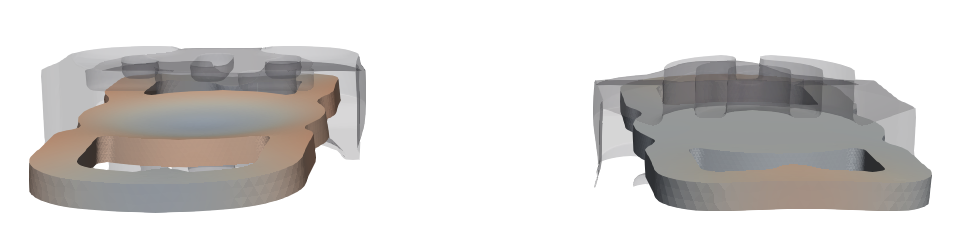
\includegraphics[width=0.235\textwidth]{figures/stills/00000_overview.png} & 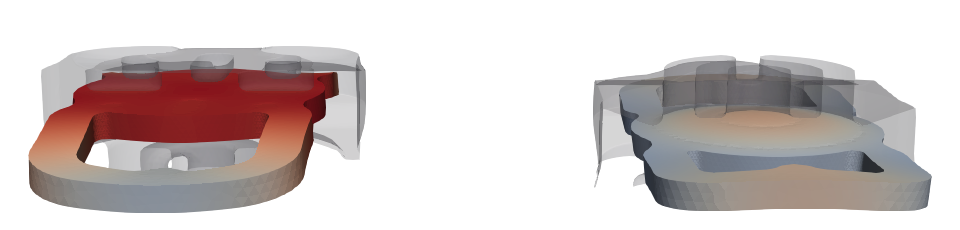
\includegraphics[width=0.235\textwidth]{figures/stills/00038_overview.png} & 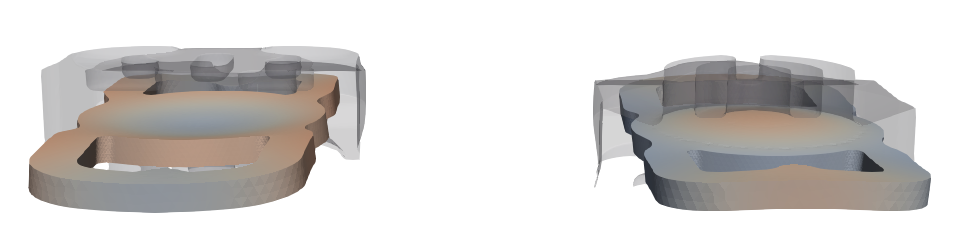
\includegraphics[width=0.235\textwidth]{figures/stills/00261_overview.png} & 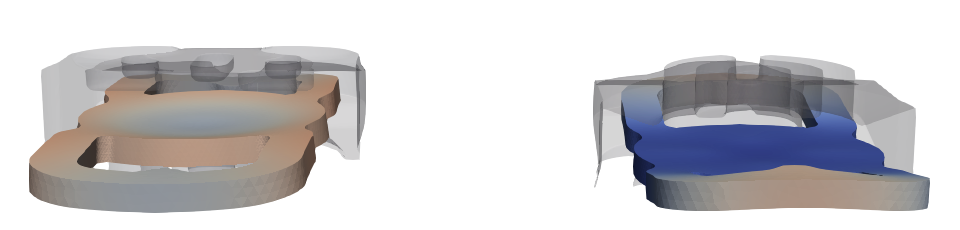
\includegraphics[width=0.235\textwidth]{figures/stills/00276_overview.png} \\
\rotatebox{90}{\scriptsize\hspace{2pt}from above} & 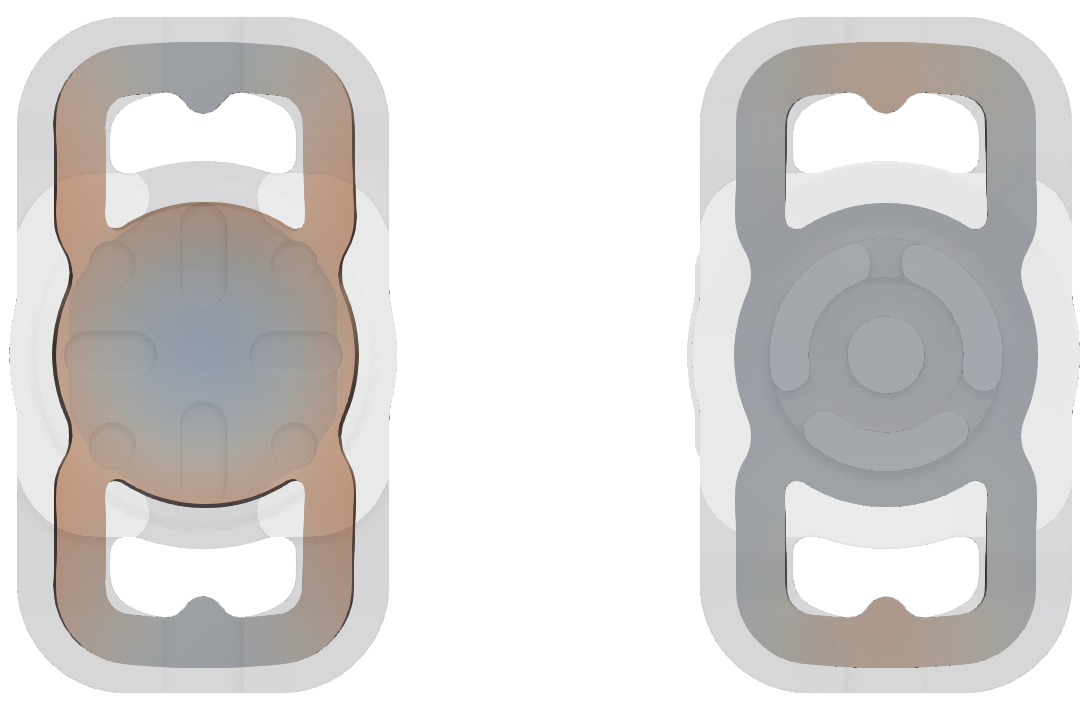
\includegraphics[width=0.235\textwidth]{figures/stills/00000_top.png} & 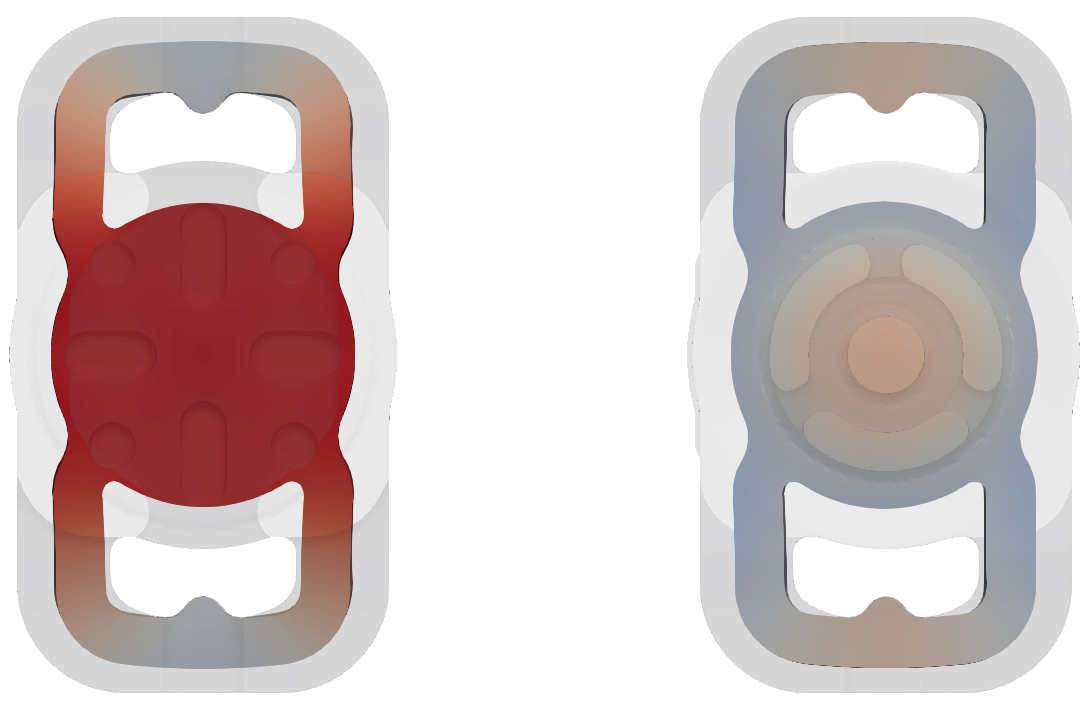
\includegraphics[width=0.235\textwidth]{figures/stills/00038_top.png} & 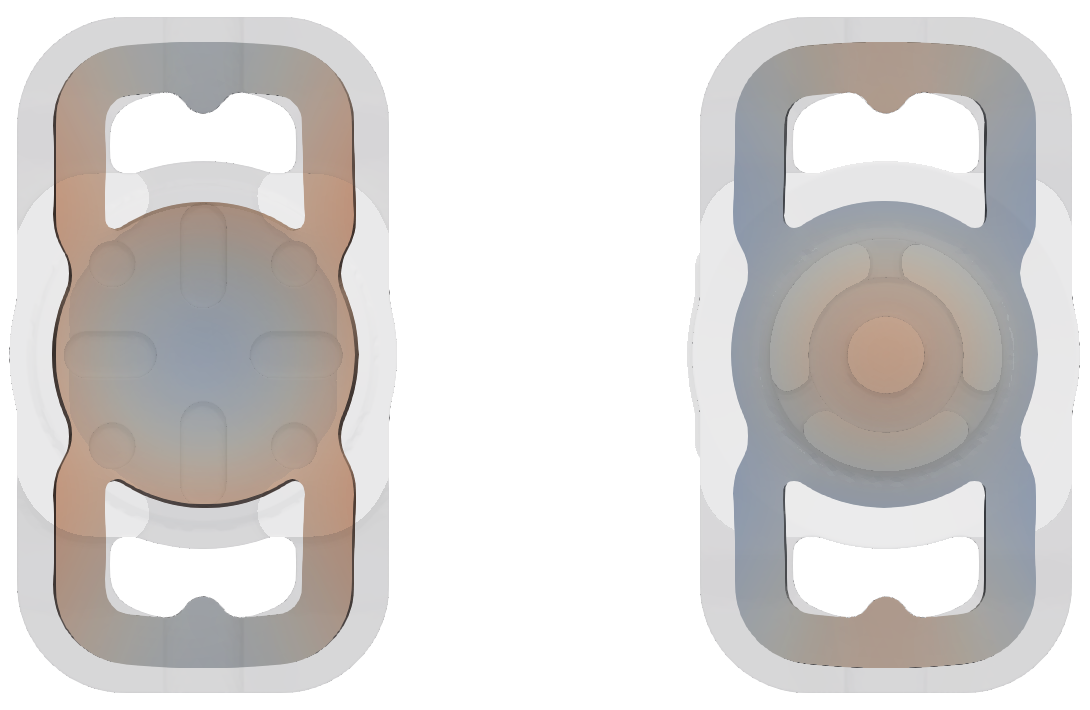
\includegraphics[width=0.235\textwidth]{figures/stills/00261_top.png} & 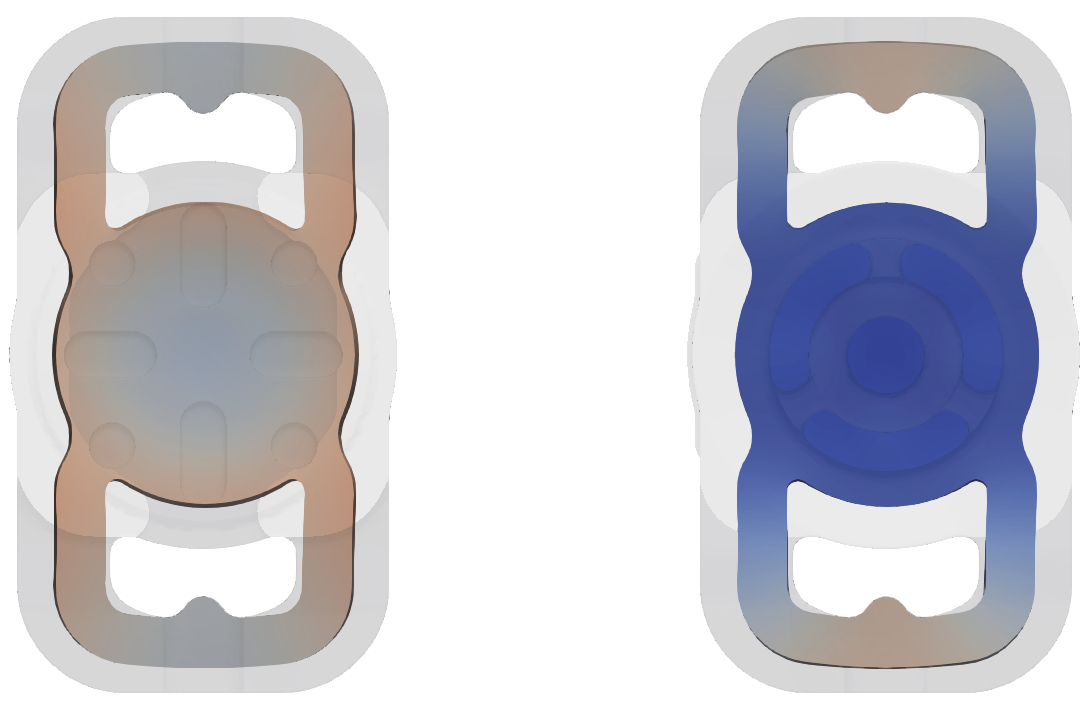
\includegraphics[width=0.235\textwidth]{figures/stills/00276_top.png} \\
\rotatebox{90}{\scriptsize\hspace{2pt}pressure valve} & 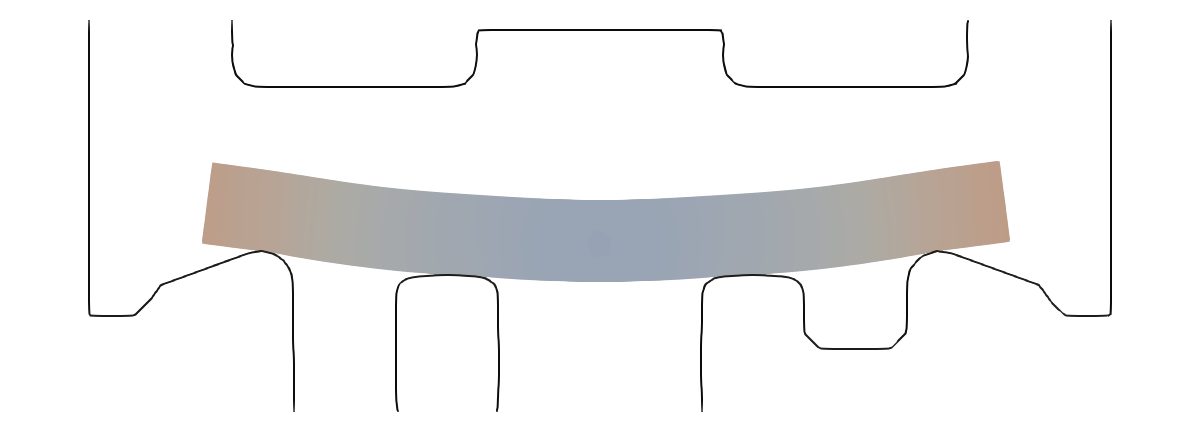
\includegraphics[width=0.235\textwidth]{figures/stills/00000_pressure_valve.png} & 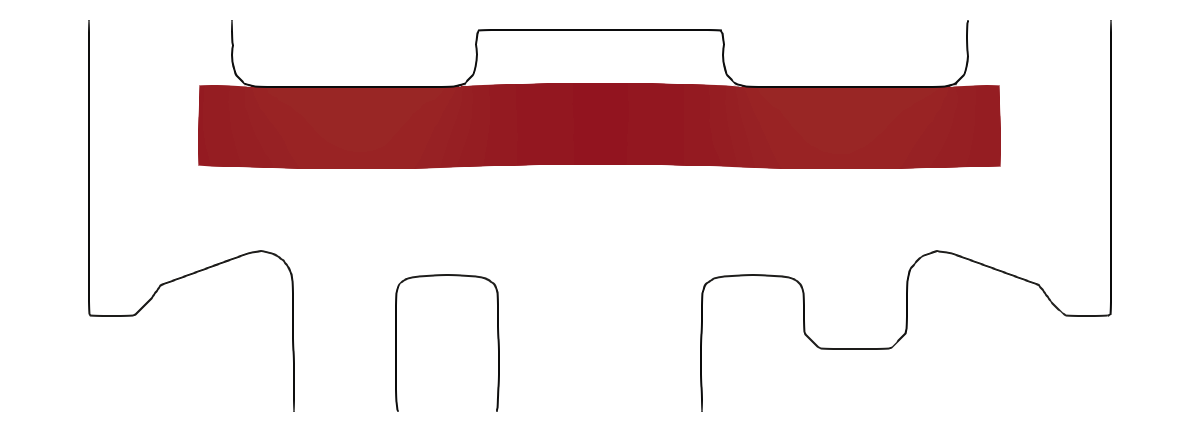
\includegraphics[width=0.235\textwidth]{figures/stills/00038_pressure_valve.png} & 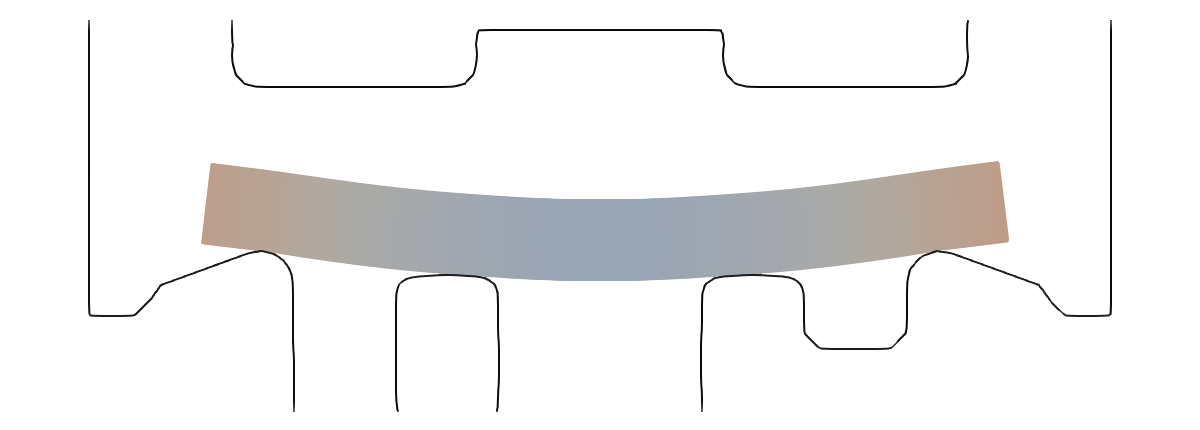
\includegraphics[width=0.235\textwidth]{figures/stills/00261_pressure_valve.png} & 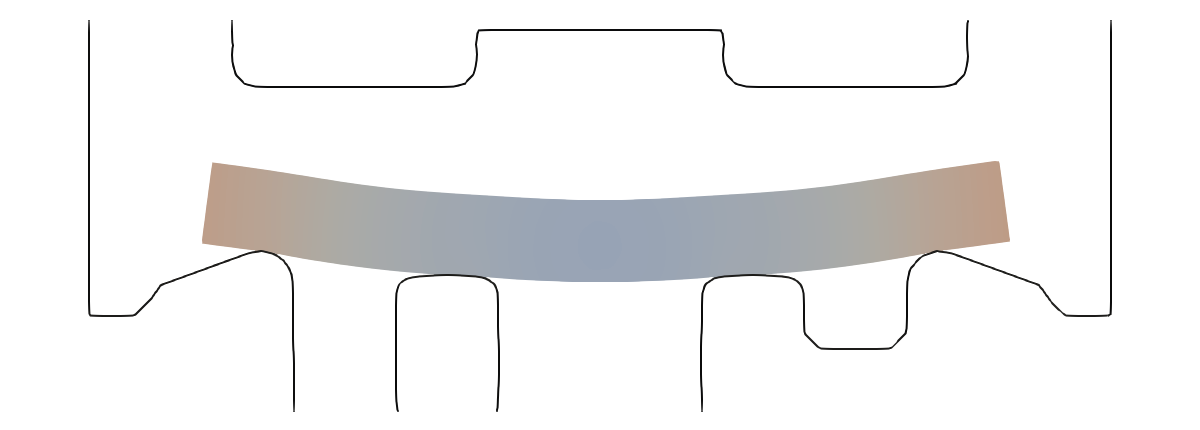
\includegraphics[width=0.235\textwidth]{figures/stills/00276_pressure_valve.png} \\
\rotatebox{90}{\scriptsize\hspace{2pt}suction valve} & 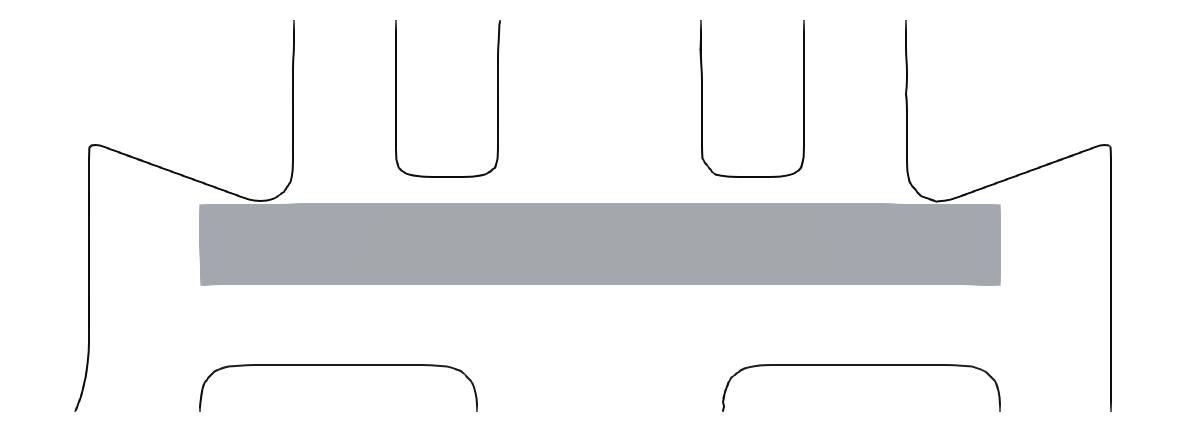
\includegraphics[width=0.235\textwidth]{figures/stills/00000_suction_valve.png} & 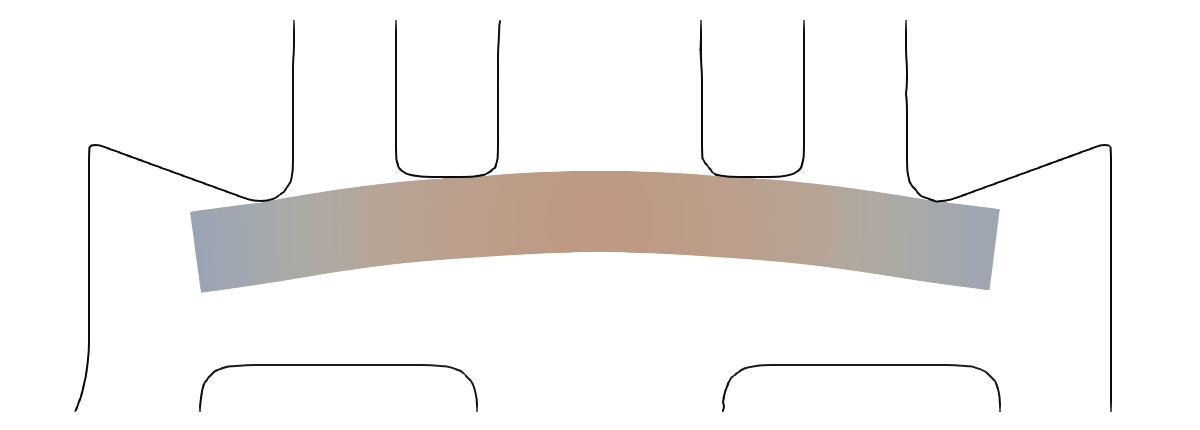
\includegraphics[width=0.235\textwidth]{figures/stills/00038_suction_valve.png} & 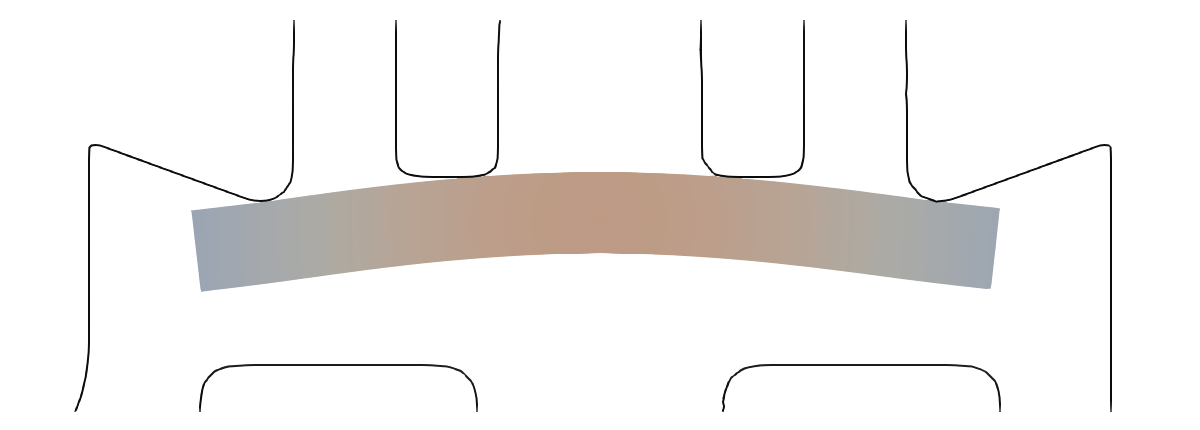
\includegraphics[width=0.235\textwidth]{figures/stills/00261_suction_valve.png} & 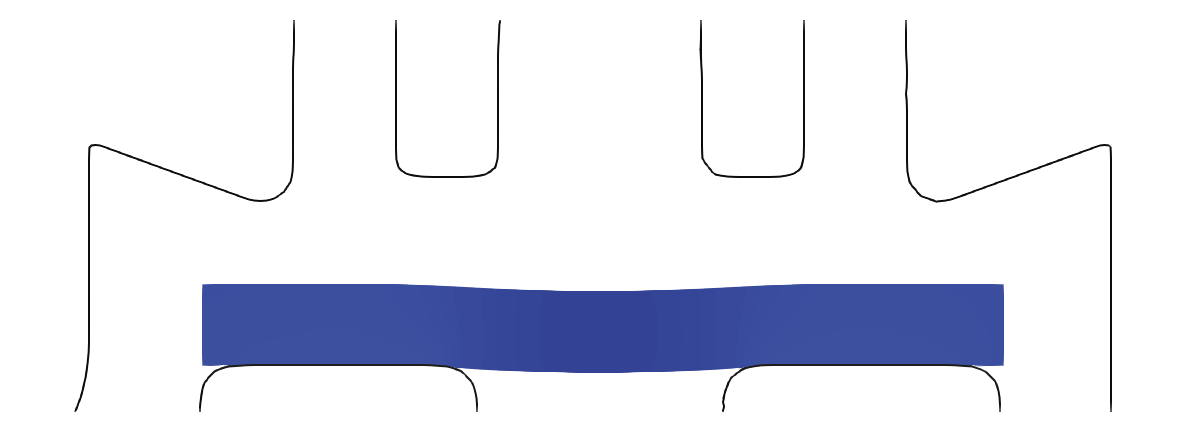
\includegraphics[width=0.235\textwidth]{figures/stills/00276_suction_valve.png} \\
\end{tabular}
\par\smallskip
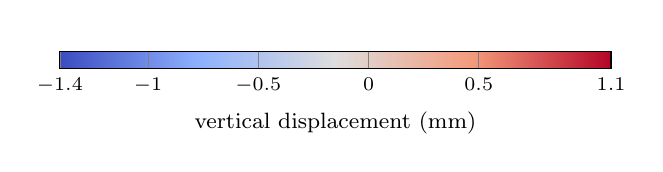
\begin{tikzpicture}
\begin{axis}[hide axis, scale only axis, width=1pt, height=1pt,
  colormap={cooltowarm}{rgb255=(59,76,192) rgb255=(141,176,254) rgb255=(221,221,221) rgb255=(244,154,123) rgb255=(180,4,38)}, colorbar horizontal,
  point meta min=-1.4, point meta max=1.1,
  colorbar style={width=7cm, height=0.22cm, xtick={-1.4,-1,-0.5,0,0.5,1.1},
    tick label style={font=\scriptsize}, xlabel={vertical displacement (\si{\milli\metre})},
    xlabel style={font=\footnotesize}}]
\addplot[draw=none] coordinates {(0,0)};
\end{axis}
\end{tikzpicture}

\caption{The valves at four instants of the first stroke, coloured by the vertical displacement
from the meshed geometry: at rest, the pressure valve on its cage, both valves seated, and the
suction valve on its stop. Overview from the front with the near half of the cavity wall removed,
the wall from above (both translucent), and each valve's section in its middle plane with the
wall's section. Rendered by ParaView from the run's raw output.}
\label{fig:stills}
\end{figure*}

\begin{table}
\caption{FF200 through \trStrokes{} strokes, \trStepsNominal{} nominal steps, on one GPU:
steps, failed attempts, Newton steps (those of failed attempts included) and time in the
QPs, in writing the output and in total. The first two runs wrote every field, the last the
displacement only.}
\label{tab:strokes}
\small
\setlength{\tabcolsep}{3pt}
%% Generated by wip/ldp_containment/python/ldp_figures.py -- do not edit.
%% Regenerate with: make figures

\begin{tabular}{@{}lrrrrrr@{}}
\toprule
 & & & & \multicolumn{3}{c}{Time (\si{\second})} \\
\cmidrule(l){5-7}
Time integration & Steps & Failed & Newton steps & QP & Writing & Total \\
\midrule
Newmark, $\gamma=0.6$ & \num{2619} & \num{1699} & \num{32299} & \num{1349} & \num{219} & \num{1675} \\
BDF2 & \num{2156} & \num{604} & \num{14484} & \num{316} & \num{167} & \num{560} \\
BDF2, all changes & \num{1807} & \num{10} & \num{9441} & \num{143} & \num{29.3} & \num{231} \\
\bottomrule
\end{tabular}

\end{table}

\begin{table}
\caption{The valves per stroke on both meshes (BDF2, all changes): opening, closing and largest
lift of the centre, the suction valve's bounce on closing not counted.}
\label{tab:valves}
\small
\setlength{\tabcolsep}{4pt}
%% Generated by wip/ldp_containment/python/ldp_figures.py -- do not edit.
%% Regenerate with: make figures

\begin{tabular}{@{}llrrrrrr@{}}
\toprule
 & & \multicolumn{3}{c}{Pressure valve} & \multicolumn{3}{c}{Suction valve} \\
\cmidrule(lr){3-5}\cmidrule(l){6-8}
Stroke & Mesh & opens & closes & lift & opens & closes & lift \\
 & & (\si{\milli\second}) & (\si{\milli\second}) & (\si{\milli\metre}) & (\si{\milli\second}) & (\si{\milli\second}) & (\si{\milli\metre}) \\
\midrule
1 & FF200 & \num{2.5} & \num{25.3} & \num{1.44} & \num{27.0} & \num{42.4} & \num{1.08} \\
 & FF200 refined & \num{2.6} & \num{25.0} & \num{1.45} & \num{27.0} & \num{42.5} & \num{1.06} \\
\addlinespace
2 & FF200 & \num{47.6} & \num{70.4} & \num{1.43} & \num{72.1} & \num{87.5} & \num{1.05} \\
 & FF200 refined & \num{47.6} & \num{70.0} & \num{1.45} & \num{72.0} & \num{87.5} & \num{1.05} \\
\addlinespace
3 & FF200 & \num{92.6} & \num{115.1} & \num{1.44} & \num{117.1} & \num{132.5} & \num{1.06} \\
 & FF200 refined & \num{92.6} & \num{115.1} & \num{1.43} & \num{117.1} & \num{132.5} & \num{1.06} \\
\addlinespace
4 & FF200 & \num{137.6} & \num{160.5} & \num{1.45} & \num{162.1} & \num{177.6} & \num{1.06} \\
 & FF200 refined & \num{137.7} & \num{160.5} & \num{1.44} & \num{162.2} & \num{177.6} & \num{1.05} \\
\bottomrule
\end{tabular}

\end{table}

\begin{table}
\caption{One change at a time, FF200 on one GPU over the first \trWindowFinish\,\si{\milli\second}
of the strokes (\trWindowStart\,\si{\milli\second} for Newton's start), each against the build
before it: steps, failed attempts, QP time and QP time per Newton step. Whole runs are not
reproducible to the bit, so their step counts can differ by a few. n.-m.\ LS: non-monotone line
search.}
\label{tab:changes}
\footnotesize
\setlength{\tabcolsep}{2.5pt}
%% Generated by wip/ldp_containment/python/ldp_figures.py -- do not edit.
%% Regenerate with: make figures

\begin{tabular}{@{}llrrrr@{}}
\toprule
 & & & & \multicolumn{2}{c}{QP} \\
\cmidrule(l){5-6}
Change & Variant & Steps & Failed & (\si{\second}) & per Newton (\si{\milli\second}) \\
\midrule
Reduction end & 2nd kernel & \num{194} & \num{65} & \num{33.4} & \num{26.5} \\
 & last block & \num{194} & \num{65} & \num{32.2} & \num{25.5} \\
\addlinespace
Tangent & float64 & \num{194} & \num{65} & \num{32.2} & \num{25.5} \\
 & float32 & \num{191} & \num{58} & \num{25.6} & \num{21.2} \\
\addlinespace
CG steps & one by one & \num{194} & \num{65} & \num{26.5} & \num{21.0} \\
 & device runs & \num{194} & \num{65} & \num{24.0} & \num{19.1} \\
\addlinespace
Newton's start & $u_n$ & \num{362} & \num{117} & \num{40.5} & \num{17.2} \\
 & $u_n+\Delta t\,v_n$ & \num{304} & \num{6} & \num{20.9} & \num{13.5} \\
 & $u_n$, n.-m.\ LS & \num{346} & \num{89} & \num{40.3} & \num{17.9} \\
 & $u_n+\Delta t\,v_n$, n.-m.\ LS & \num{300} & \num{0} & \num{21.5} & \num{14.0} \\
\bottomrule
\end{tabular}

\end{table}


\begin{figure*}
\centering
%% Generated by wip/ldp_containment/python/ldp_figures.py -- do not edit.
%% Regenerate with: make figures

\setlength{\tabcolsep}{1pt}
\renewcommand{\arraystretch}{0.6}
\begin{tabular}{@{}cccc@{}}
 & \footnotesize overview, $t=\SI{3.8}{\milli\second}$ & \footnotesize pressure valve, $t=\SI{3.8}{\milli\second}$ & \footnotesize suction valve, $t=\SI{27.5}{\milli\second}$ \\
\rotatebox{90}{\scriptsize\hspace{2pt}FF200} & 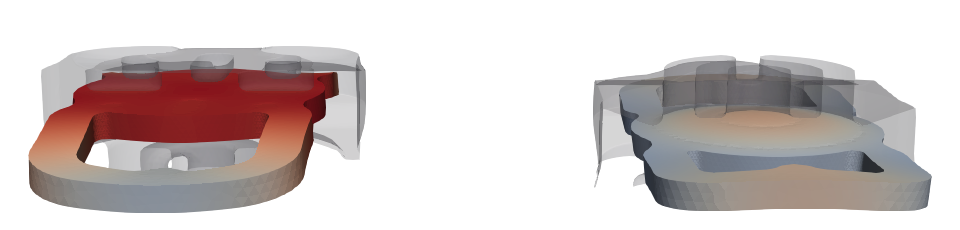
\includegraphics[width=0.315\textwidth]{figures/stills/00038_overview.png} & 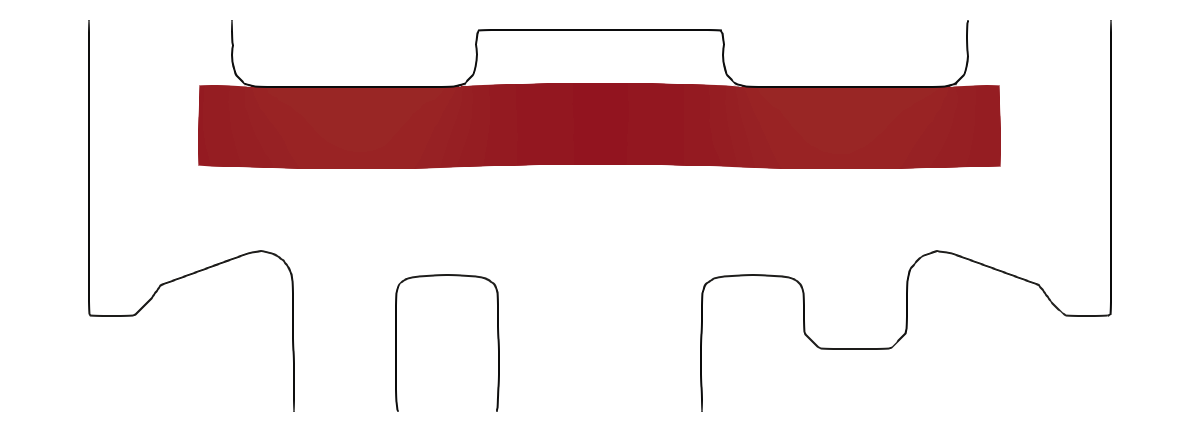
\includegraphics[width=0.315\textwidth]{figures/stills/00038_pressure_valve.png} & 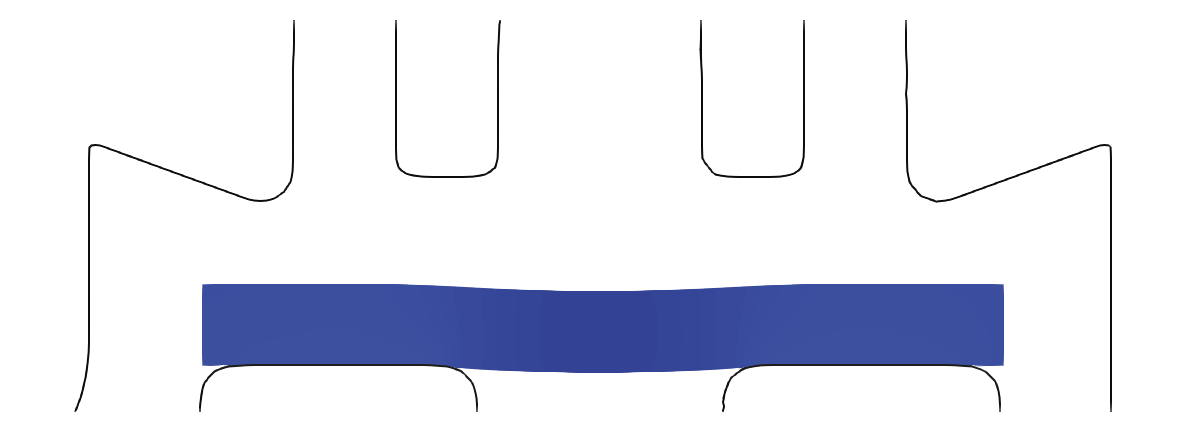
\includegraphics[width=0.315\textwidth]{figures/stills/00276_suction_valve.png} \\
\rotatebox{90}{\scriptsize\hspace{2pt}FF200 refined} & 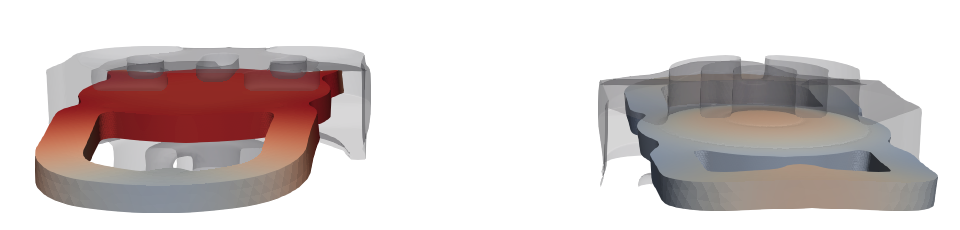
\includegraphics[width=0.315\textwidth]{figures/stills_refined/00042_overview.png} & 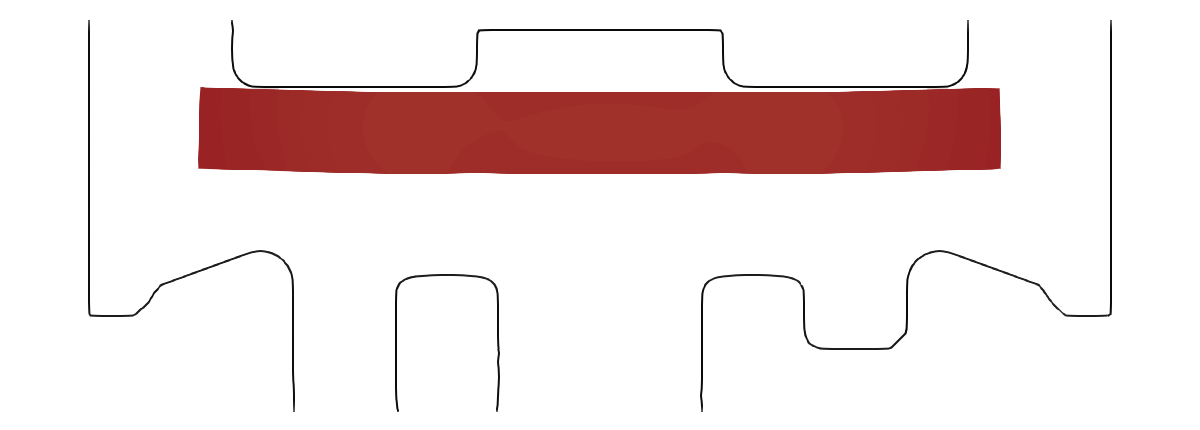
\includegraphics[width=0.315\textwidth]{figures/stills_refined/00042_pressure_valve.png} & 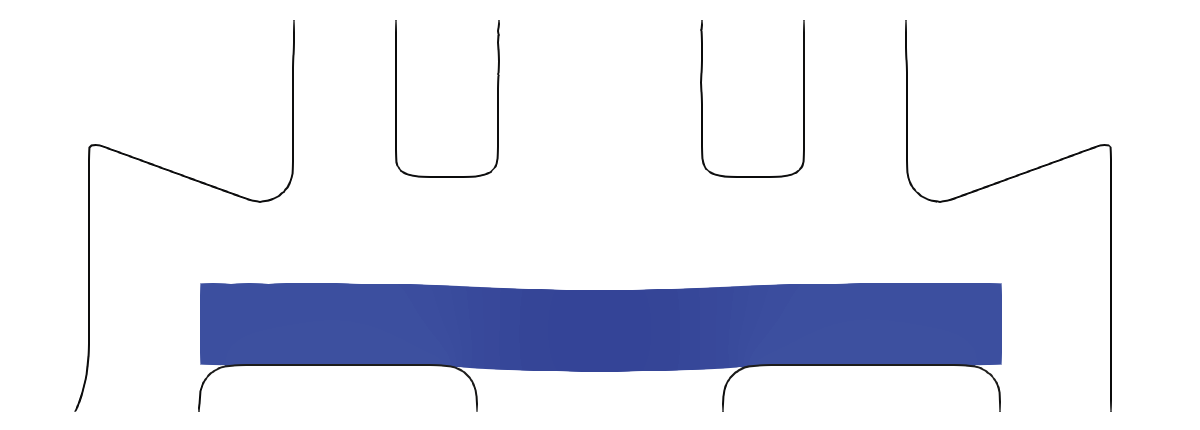
\includegraphics[width=0.315\textwidth]{figures/stills_refined/00312_suction_valve.png} \\
\end{tabular}

\caption{FF200 (top) and FF200 refined (bottom) at the same instants of the first stroke: the
pressure valve on its cage, overview and its section, and the suction valve on its stop, its
section; coloured as Figure~\ref{fig:stills}.}
\label{fig:resolutions}
\end{figure*}


\section{Limitations}

In the single-process runs \qpCappedClause{}. The Newton budget
of \unconvergedCases{} ends before the KKT tolerance is reached. The comparison with utopia samples
the distance field trilinearly for both states, so penetrations below the grid's interpolation
error are not resolved. All measurements are on one system; utopia was not rerun on it.
The pump strokes of Section~\ref{sec:strokes} borrow FP70's chamber pressure for FF200, apply it as
a dead vertical traction on a disc, ignore the fluid between the valve and its seat, and hold the
valves by the cavity alone; the split $C_{01}/C_{10}=4$ is assumed, and the strokes were run
without a step-size study.

\bibliographystyle{ACM-Reference-Format}
\bibliography{refs}

\end{document}
